%!TEX TS-program = xelatex
%!TEX encoding = UTF-8 Unicode

\documentclass[a4paper,twosided,10pt]{book}

\usepackage[a4paper,textwidth=42em,tmargin=25mm,bmargin=27mm,bindingoffset=17mm]{geometry}
\usepackage[dvipsnames]{xcolor}
\usepackage{calc}
\usepackage{amsmath,xltxtra,xunicode}
\usepackage{titlesec}
\usepackage{fontspec}
\usepackage{fancyhdr}
\usepackage{datetime2}
\usepackage{wasysym,oz,pxfonts,txfonts}


\usepackage{tcolorbox}
\usepackage{qrcode}
\usepackage{indentfirst}


\usepackage[PunctStyle=plain,RubberPunctSkip=false]{xeCJK}
\defaultCJKfontfeatures{Script=CJK}
\XeTeXlinebreaklocale "zh"
\XeTeXlinebreakskip = 0pt plus 1pt

% =========================================
\usepackage[hidelinks]{hyperref}
\hypersetup{
    colorlinks=false,
    pdftitle={Shell Beach (2022)},
    pdfpagemode=FullScreen,
}
\usepackage{listings,paralist}
\setdefaultleftmargin{3em}{2em}{1em}{1em}{1em}{1em}

\usepackage{enumerate,enumitem}
\usepackage{longtable}
\usepackage{tabu}

\usepackage{tocloft}
\renewcommand{\contentsname}{\sffamily{目录}\vspace{30pt}\hrule\vspace{2pt}}
\renewcommand{\cftchapfont}{\vspace{0pt}\mdseries\rmfamily}
\renewcommand{\cftchappagefont}{\vspace{0pt}\mdseries\rmfamily}
\setlength{\cftbeforechapskip}{0pt}
\newcommand{\mybookpart}[1]{
    \addcontentsline{toc}{chapter}{\linebreak\textbf{\Large#1}\vspace{7pt}}
    \part*{#1}
}

\usepackage{graphicx}
\graphicspath{ {/home/neruthes/DEV/shellbeach-book/img/} }

\usepackage{etoolbox}
\patchcmd{\quote}{\rightmargin}{\leftmargin 2em \rightmargin}{}{}

\usepackage[bottom]{footmisc}
\renewcommand*{\footnotelayout}{\footnotesize\rmfamily\fontspec{Noto Serif CJK SC}\CJKfontspec{Noto Serif CJK SC}}

% \usepackage[sfdefault]{inter}
\usepackage[OT1,T1]{fontenc}
% \renewcommand*\familydefault{\ttdefault}

% Bad roman fonts: Times New Roman, NewComputerModern, Noto Serif, Theano Modern, Spectral
% Good roman fonts: Domitian, Palatino, QTPalatine

% \usepackage{kpfonts}
% \usepackage{TheanoModern}
% \usepackage{txfonts}

\setmainfont{QTPalatine}
\setromanfont{QTPalatine}
\setsansfont{Inter}
\setmonofont{Noto Sans Mono Condensed}
\setCJKmainfont{Noto Serif CJK SC}
\setCJKromanfont{Noto Serif CJK SC}
\setCJKsansfont{Noto Sans CJK SC}
\setCJKmonofont{Noto Sans CJK SC}


\title{Shell Beach (2022)}
\author{白色灯塔先生}
\date{2022}
% =========================================

% =========================================
% START CORPORATION CONFIG
% \setlength{\parindent}{0pt}
\setlength{\parindent}{2em}
\setlength{\parskip}{8pt}
% END CORPORATION CONFIG
% =========================================

% =========================================
% START COMMON STYLESHEET

% END COMMON STYLESHEET
% =========================================




\pagestyle{fancy}
\renewcommand{\headrule}{}
% \fancyhf{}
% \fancyhead[LE,RO]{\sffamily Shell Beach}
% \fancyhead[LO,RE]{\sffamily \thechapter}
% \fancyhead[C]{}
% \fancyfoot[LE,RO]{\itshape\small{\thepage}}
% \fancyfoot[LO,RE]{}
% \fancyfoot[C]{}


\fancypagestyle{plain}{
    \renewcommand{\headrulewidth}{0pt}
    \renewcommand{\footrulewidth}{0pt}
    \fancyhf{}
    \rhead{}
    \chead{}
    \lhead{}
    \rfoot{}
    \cfoot{}
    \lfoot{}
}
\fancypagestyle{fancy}{
    \fancyhf{}
    \renewcommand{\headrule}{}
    \fancyhead[LE,RO]{\small\sffamily Shell Beach}
    \fancyhead[LO,RE]{\small\sffamily \#2022-\leftpad{\thechapter}}
    \fancyhead[C]{}
    \fancyfoot[LE,RO]{\small{\thepage}}
    \fancyfoot[LO,RE]{}
    \fancyfoot[C]{}
}





\makeatletter\@addtoreset{chapter}{part}\makeatother%

\newcommand{\useimg}[1]{
    \noindent\begin{minipage}{\linewidth}
        \centering
        \vspace{3pt}
        \includegraphics[width=\textwidth-8em,keepaspectratio,height=0.5\textheight]{#1}
        \vspace{3pt}
    \end{minipage}
}
\newcommand{\midnote}[1]{
    \noindent{\sffamily\footnotesize\hfill#1\hfill}
}
\newcommand{\pozhehao}[0]{%
    {\fontspec{FandolSong}\CJKfontspec{FandolSong}——}%
}
\newcommand{\twochartab}[0]{%
    {\hspace{2em}}%
}
\newcommand{\ardate}[2]{
    \noindent\begin{minipage}{\textwidth}
        \noindent{%
            \ttfamily\small#1%
        } \hfill {%
            \footnotesize
            \sffamily
            \fontspec{Noto Sans Mono Condensed}
            \href{https://mp.weixin.qq.com/s/#2}{https://mp.weixin.qq.com/s/#2}%
        }%
    \end{minipage}

    \vspace{8pt}
    \hrule
    \vspace{30pt}
}
\newcommand{\blockquote}[1]{
    \begin{quote}
        \normalsize
        \rmfamily
        % \fontspec{GFS Bodoni}
        % \fontspec{FandolKai}
        \fontspec{NewComputerModern}
        \CJKfontspec{FandolKai}
        % \itshape
        #1
    \end{quote}
}
\newcommand{\blockquotesource}[3]{
    % $1=title $2=author $3=year
    \par{\footnotesize\sffamily
        \hfill
        #1
        \hspace{0.5em}·\hspace{0.5em}
        #2
        \hspace{0.5em}·\hspace{0.5em}
        #3%
    }%
}
\newcommand{\citebook}[1]{
    \par{\small\sffamily
        \hfill
        #1
    }\par
}
\newcommand{\dialoguelist}[2]{
    % $1=namewidth $2=content
    \begin{description}[widest=A#1,leftmargin=*,font=\mdseries\rmfamily\CJKfontspec{FandolKai}\itshape]%
        #2%
    \end{description}%
}
\newcommand{\dialoguelistthin}[2]{
    % $1=namewidth $2=content
    \blockquote{%
        \dialoguelist{#1}{#2}%
    }%
}
\newcommand{\dialogue}[2]{
    \item[#1] \textrm{#2}%
}
\newlength{\dialogueseplinenamewidth}
\newcommand{\dialoguesepline}[2]{
    % $1=actorNameColWidthExample $2=content
    % \item \textsf{\hfill\footnotesize #2\hfill{\color{white}AA#1}}
    \settowidth{\dialogueseplinenamewidth}{#1}
    \item \begin{minipage}{\linewidth-\dialogueseplinenamewidth-1em}
        \sffamily\centering\footnotesize
        #2
    \end{minipage}
}
\newcommand{\threestars}[0]{
    {*\hspace{1em}*\hspace{1em}*}
}
\newcommand{\tristarsepline}[0]{
    \noindent\begin{minipage}{\textwidth}
        \center
        \noindent
        \threestars
    \end{minipage}
}
\newcommand\ifootnote[1]{%
    \begingroup
    \renewcommand\thefootnote{}\footnote{#1}%
    \addtocounter{footnote}{-1}%
    \endgroup
}
\newcommand{\makedraftdeclaration}[0]{
    \clearpage
    
    \hspace{0.5\linewidth}
    \vspace{0.4\textheight}
    
    {\hfill\sffamily{以下为尚未完工的草稿}\hfill}
    
    \vfill
    
    \clearpage
}
\newcommand{\leftpad}[1]{\ifnum#1<100 0\ifnum#1<10 0\fi\fi#1}
% \newcommand{\leftpad}[1]{\ifnum\thechapter<100 0\ifnum\thechapter<10 0\fi\fi\thechapter}


% \titleformat{\chapter}[display]{\huge\bfseries}{\raggedright\mdseries\normalsize\fontspec{SF Pro Text}Article \thechapter\linebreak}{0pt}{\LARGE\bfseries}
\titleformat{\chapter}[display]{\small\mdseries\rmfamily\fontspec{Noto Serif CJK SC}}{\raggedright\mdseries\large\ttfamily \#2022-\leftpad{\thechapter}\vspace{10pt}}{0pt}{\Large\bfseries}



\linespread{1.16}



\begin{document}
\raggedbottom
\pagestyle{empty}
\rmfamily\mdseries\normalsize



\newgeometry{hmargin=50mm,tmargin=50mm,bmargin=50mm}% For A4 paper
% \newgeometry{hmargin=20mm,tmargin=30mm,bmargin=30mm}% For A5 paper
\begin{titlepage}
    \center

    \parindent=0pt
    % \sffamily
    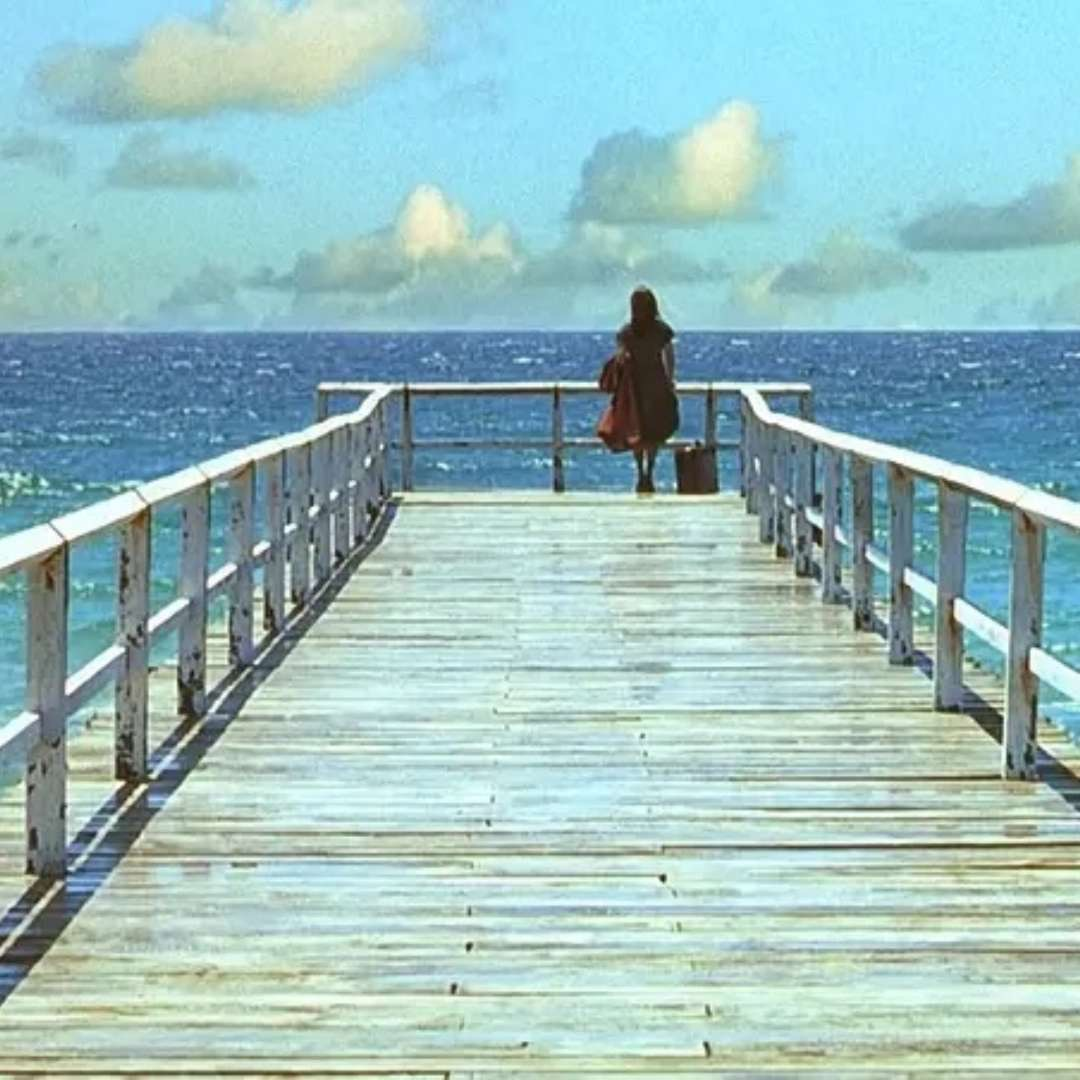
\includegraphics[width=60mm]{shellbeach-avatar.jpg}
    \vspace{20pt}

    \Huge
    \fontspec{Noto Serif Display}
    {\bfseries{Shell Beach}}

    \vspace{20pt}

    \normalsize
    % 二零二二年度公众号文章合集\\
    % 持续更新中

    % \fontspec{Playfair Display}
    % \fontspec{Libre Bodoni}\scshape
    \fontspec{Playfair Display}\scshape
    % \fontspec{Calluna}\scshape
    % \fontspec{Tinos}\scshape
    % \fontspec{Theano Didot}\scshape
    \Large
    Channel Article\\
    Annual Collection\\
    % 2022
    
    % \Huge{\bfseries{}2022}

    \vspace{25pt}
    \Huge\fontsize{36pt}{36pt}\selectfont
    \fontspec{Noto Serif Display}
    {\mdseries{2022}}
    
    % \fontspec{Noto Serif Display}
    % \LARGE{2022}

	\vfill

	\sffamily
    \normalsize
    白色灯塔先生

\end{titlepage}
\newgeometry{textwidth=42em,tmargin=25mm,bmargin=27mm,bindingoffset=17mm}% For A4 paper
% \newgeometry{textwidth=32em,tmargin=20mm,bmargin=15mm,bindingoffset=13mm}% For A5 paper


\rmfamily
\normalsize





% \chapter*{前言}

% Hello world!

\cleardoublepage

\setcounter{tocdepth}{0}
\textmd{\sffamily\tableofcontents}
\cleardoublepage
\setcounter{page}{1}


% \pagestyle{myheadings}
% \pagestyle{plain}
\pagestyle{fancy}
% ======================================
% BEGIN LIST
\mybookpart{第一季度}

\chapter{随笔 | 元旦,生气,冲突,意义}

\ardate{2022-01-03}{xgeE9XaLnaKGN3xmmsRDPA}


元旦假期,我去了另一个城市找朋友L玩。在假期的第二天,我和朋友和朋友L所认识的另一位男生M一起约去艺术展观展。

我们先是吃了顿午饭,午饭的大多数时候都是我听着朋友L和男生M在聊天,然后我们去了那个艺术展。在逛艺术展时,朋友L在男生M不在附近的情况下跟我说:“看完展我们就回去睡个午觉,然后晚饭叫个外卖。”后来,逛展越逛越晚,在快到下午五点时,男生M提议我们去吃晚饭。我知道朋友L只想回家休息,然后我看朋友L对此是否会有什么反应,但朋友L只是把手机摆在脸前玩,没有什么回应。然后男生M便开始在手机上搜附近的餐厅。我想到朋友L想早点回家,然而现在已经离朋友L的设想(看完展就回去睡个午觉)已经相差甚远,所以我在手机上找了几家艺术展附近的餐厅向男生M提议。但男生M并不想去那些餐厅,然后找了一家需要坐地铁去的有一定距离的餐厅。在去餐厅的路上,朋友L依然只是在玩着手机。

当去到那家餐厅吃饭时,朋友L依然全程用手机遮挡着脸,全神贯注地玩着手机。在我和男生M吃得尽兴,同时开始熟起来地聊天时,男生M开始注意到朋友L一直玩着手机有点奇怪,便向朋友L招手,想要引起他的注意,但朋友L一直没有回应。在和男生M聊天的过程中,我开始觉察到他从午饭一直到晚饭的过程中,似乎都很主动地承担活动组织者的角色,会去记住谁是哪里人、喜欢吃什么、不喜欢吃什么、有什么忌口,会去找性价比高又好吃的餐厅、控制成本(人均消费)。我在午饭的时候便向他提出这一点,他发现这更像是他在工作方面的习惯。

吃晚饭时,男生M聊到他生活在公司的宿舍里,没有太多自己的空间。这让我想起刚刚在逛礼品店的时候,男生M看见了自己喜欢的东西,我问他他打算买吗,他说他还不打算,因为他住的宿舍没有这样的空间能放那件物品。吃着吃着,店员上了一杯柠檬茶,另外还送了另一瓶瓶装的柠檬茶。他想让我把瓶里的柠檬茶喝了,我问他:“你是想要这个瓶子?” 他回答说:“是的。”我接着问:“你是想用这个瓶子干些什么吗?”他说:“打算用来种绿植,装土壤。”我回应道:“虽然你说你没有太多自己的空间,但你好像依然会让一些属于你自己的东西‘生长’出来。”他回答说:“是啊,毕竟还是要过生活的嘛,就像自己一个人吃饭也要找一些性价比高又好吃的餐厅。”然后他聊到他并不喜欢呆在宿舍的生活,所以到了周末就会尽可能出来玩,多在外面逛,而不是呆在宿舍里,因为一呆很可能周末就过去了。这让我回想起我以前在大学时的宿舍生活,我在那个当下能理解他想要多在外面度过时间的念头以及这个念头的背景。

聊着聊着,男生M说他想去看一下附近的一家有猫的饮品店,我问朋友L想去吗,他说他不想,但声音小得只有我能听到。吃完饭后,男生M在找那家饮品店在哪,朋友L在跟着他走的时候突然大声地说了句:“我不要跟你玩了!”然后一个人转身走向离开商场的方向。我和男生M跟了过去,男生M问我他怎么了,我说:“他可能早就想回家了。”

在地铁里,和男生M匆匆道别后,我和朋友L坐在地铁里,我问朋友L:“你会想他(男生 M)在定行程的时候多关心一下你吗?”朋友L回答说:“他总是会在计划好的行程后加更多东西,我一开始就说好只是约艺术展。(他)不像你,你问了我是不是想去饮品店。”我说:“如果你可以早一点跟他表达这一点,说不定他就能更早地知道(这一点)。不过,他下一次估计也就知道了吧。”朋友L回答说:“他总是这样,又不是一次两次了。”我回答道:“噢,那这可能是他的一种模式吧。”

我猜想到男生M为什么会有这一模式:因为不想呆在宿舍而想多在外面逛。但出于这样的背景和意图,男生M可能在定行程的过程中忽视了同行人的想法和意见。另一方面,朋友L当时的回答“我不要跟你玩了!”听起来更像是一个小朋友会说的话,或者说这是他内心更偏向小朋友的部分、小朋友的自我所说的话,我猜想这可能是因为朋友L在那个当下感受到了小时候所曾经感受到的感觉,猜想到小时候的他说不定经历了某些创伤,一些不被他人关心和重视甚至是不被他人“看到”的创伤。同时,把手机摆在脸前来回避与外界的互动的行为也很像小朋友生闷气的表现。

当朋友L生气时,我的第一反应是回避,因为在我的原生家庭里,回避生气的人意味着少挨打。但我很快意识到自己开始表现出回避甚至是有点讨好攻击者的行为,并将焦点转向朋友L,试图去设想为什么朋友L会生气。我想起近两个月前开始学的人本课程内容里,当事人的痛苦的背后往往意味着TA所珍重的意义的受创。所以我想知道,朋友L的生气背后,那个受伤的部分背后所代表的他所珍重的会是怎样的意义。当我得知他重视的是他人对他的关心后,在之后和他的相处里,我也逐渐意识到,朋友L很少会主动与人(包括我)产生连接,很少主动关心他人的内心事物,而只有在他人开始关心他内心的事物时,他才会去反之关心他人。

\tristarsepline

以前的我(特别是小时候的我)总是回避攻击者,甚至讨好攻击者,认为任何的不和谐和冲突甚至是攻击都是自己所不能忍受的、“不好”的事情。但这次我意识到,这些冲突背后有着它们的意义、暗藏着那些身边的他人所珍重的意义、他们更为内在的事物。冲突并不是一件“不好”的事情,因为在冲突背后有着许多真实的自我,那些当事人可能早已遗忘或隐藏起来的自我。冲突反而能让我更好地理解对方、看见对方、看到对方所珍重的意义。


\useimg{aimg/2022-0103-1.jpg}

\useimg{aimg/2022-0103-2.jpg}

\useimg{aimg/2022-0103-3.jpg}

\useimg{aimg/2022-0103-4.jpg}


\chapter{自我探索 | 14}

\ardate{2022-01-04}{Jx-QEWQm96UFDAmA3jMllg}


进入咨询室后,我确定了一下我最想要说的是什么,然后开始说:“在上一次咨询结束后,我感觉到一股悲伤,一种像是放弃了自我的悲伤。我感觉在上一次咨询里,我只是遵循着你在上上次咨询的提议\pozhehao{}无意识地说些什么,而没有做我自己。

我甚至会有一种被操控的感觉。在上上次咨询,你问我:‘如果不带准备地来咨询,你设想会发生些什么?’我说:‘可能我会继续无意识地说下去。’在我说完那句话后,我才突然意识到,这更像是你想说的话,但却通过我来让我自己说出这句话。其实在之前的咨询里,我也发现了类似的可能带有操控性的引导,比如说在之前我好奇你的穿着服装背后是否意味着你的生活里存在着某些高光时刻时,你引导我对你的生活进行了设想,一些你既不会去承认也不会去否认的设想。我想这可能是你的一种防御方式,但我能理解那时候为什么你想要这么做\pozhehao{}毕竟你想避免暴露自己的生活。但我难以接受你在上上次咨询用这样的方式来引导我说出你自己想说的话。然后我想了一下上上次咨询的背景:那时候我提出我想要结束咨询,而你不想‘放我走’。当想到那个背景时,我大概能理解为什么你会有这样的意图\pozhehao{}将咨询引向新的方向。但我觉得你可以直接提出这个建议,比如说:‘不如我们可以试着让你不带准备地来咨询,看之后会发生些什么’,但你并没有直接这样提议,而是通过一种隐晦的方式来让我说出你想说的话,所以我才会有一种被操控的感觉。”

咨询师回应道:“那种被操控的感觉会让你联想到什么吗?”我继续说:“嗯,我会联想到小时候被母亲、被外婆操控着我穿什么、吃什么、喜欢吃什么、不喜欢吃什么、我对外界的冷热的感知、我对自己的性格的认知。比如说,读小学时有一次去观展,我妈在我出门前让我穿了很多衣服,但那天很热,不过我并没有脱衣服,而是一直闷热到放学回家。一方面,我觉得很热,但另一方面,我妈说我不热。后来读到心理学方面的书籍时,我才知道这种认知操控所导致的矛盾心理是会引发精神疾病的。而且小时候我妈和我外婆都很喜欢在饭桌上塞东西给我吃,我那时候的反抗方式是在吃得很饱得时候把胃里的食物直接吐在饭桌上。”咨询师问:“这种吐的方式频繁吗?”我回答到:“只是小时候的偶尔几次,后来我就开始学会拒绝了。”(我想咨询师可能是想到厌食症和催吐行为的可能性吧)

咨询师开始联想到:“我有留意到刚刚你在描述的时候经常会用一个词:‘硬塞’,我在想,你在咨询一开始所说的我的‘引导’,会不会也给你一种像是我在‘硬塞’一些东西给你的感觉?”我思考了一下,回答道:“Em……会像是塞,但不是硬塞,而更像是一种很隐晦地暗自地塞。”

我停顿了下,回顾了一下刚刚的过程后,继续说:“其实现在当我将这些秘密说了出来,我感觉很释怀,而且好像我也并不需要知道事情的对错。我在前一两个月也向前任坦白了一些我所知道的他的秘密……(此处省略某些关于亲密关系背叛的秘密)……当我把这些事情告诉前任后,我好像也不需要他的承认或否认了。”

咨询师回答说:“我会有点好奇为什么会释怀?”我思考了一下,并说:“Em……就好像我承担了很多不属于我自己的部分,比如说一些关于前任的破事,然后我将这些不属于我的部分排了出去,扔回给了对方。无论对方是自己解决还是怎样的,我不再需要为对方承担责任、不再需要承担那些不属于我的部分。这让我感到自我完整性。我不需要担心彼此的关系会变成怎样,我只是做我自己就足够了。”

咨询师在听完后回应道:“听到这里,我还挺为你感到高兴的。同时,我也会好奇,为什么你会选择现在把这些秘密说出来,因为你好像在咨询的一开始就能看见很多我没有看见的事物。”我笑了下,继续说道:“以前的我会不敢说出这些秘密,因为担心这些秘密会破坏关系。而当和前任分手后,就更加没有说出这些秘密的必要性了,因为关系已经无法挽回。但现在我开始意识到,我保留着的这些秘密其实会损害我的自我完整性的,就好像我默许着这些事情的发生一样。而当我把这些秘密排出去后,我感到更加释怀了。而且,凭什么要我为对方的破事负责!

当我在咨询里把这些秘密说出来时,我不需要担心被你所攻击或无视或怎样的,而如果我在咨询之外的人际关系里这么做,很可能会遭到对方的攻击或无视或冷淡地对待。

这些秘密就像是咨访关系里的刺,如果我不将这些刺挑出来,不去面对这些东西,那么我们能说的事情也会越来越少,就像和前任的关系一样,能和他说的事情越来越少,因为我很怕触碰到那些我不敢去面对的雷区\pozhehao{}有关亲密关系的背叛的那些秘密。后来我们能说的话越来越少,而且两人的关系早已说不上是亲密了。我不想我们的咨访关系也变成这样,我不想像之前好几次的咨询那样只是聊一些表面的内容。而当我能看见这一点时,我便开始向你提意见,想将关系变得更深更广。而且这么做的效果好像还蛮好的?至少我的自我感觉很好~

我想,在咨询里,我开始逐渐看见我所做的事情,原来我之前就有这么做过,就有对前任这么做过,而且我开始逐渐看清这样的做法的脉络。”

咨询师问:“那你之前会有这样的经历或感觉吗?”我回答说:“嗯,有的。之前我在写作的时候能深挖到感觉背后的经历、起源和脉络。但感觉本身是不受我控制的,而这种(将秘密说出来)的做法是我能够控制的。

其实我在咨询一开始的本意只是想澄清在上上次咨询里可能存在的操控的部分。而在你的引导下,我好像将这个部分和自己的童年与前任的经历串联在了一起。”

咨询师问:“这会给你一种怎样的感觉吗?”我回答道:“一种很强的效能感。”咨询师回应:“好像一种你在掌控着主权的感觉。”我感觉了一下,回答说:“嗯。不过我想之后的咨询我们还是会回到平等的地位。因为好像只有在平等的地方,甚至是像上上次咨询我提出想要结束咨询时,我们在彼此抗衡的过程中,一些真实东西才会冒出来,一些很隐晦但又很真实的东西冒了出来。”

咨询师说:“好像你很看重‘真实’。”我回答说:“嗯。因为如果不真实的话,彼此的关系很可能会像和前任的关系一样越走越窄,在不知道发生了些什么事情的情况下关系就结束了。我并不想这样,我想在关系里做真实的自己,无论这段关系会变成怎样。

我也会想到,之前我说我感觉我在咨询里没有什么话好说,所以想结束咨询。这让我想到,这会不会是因为在咨询的环境里没有足够的空间让我创造出属于我自己的东西。

当回顾我们的咨询历程,在咨询的过程中,我好像越来越擅长处理一些看不见的东西,或者说越来越能够觉察或认知到这些部分,觉察或元认知的能力越来越强,而且应对环境的能力也还不错?同时,我也开始发现,在咨询的历程里,咨询的焦点好像逐渐从我的身上转移到了我们彼此的关系上,而且这一次的咨询完全起源于上上次咨询的那个带有操控性的引导。而我在应对我们彼此之间发生的事情的能力也在不断提升,开始在创造一些属于我自己的应付方法。”

咨询师回答道:“好像你能看见很多我没有看见的部分,然后你会将它们拿出来说。”我回想了下,回答道:“嗯,是的。但我也会在想,这不是咨询师的工作吗?这不是你的工作吗!”

咨询师笑了笑,我也笑了起来,然后我继续说:“不过我相信这不仅仅对于我,对于你而言,你也能在这个过程中有更多关于自我方面的成长。不然如果其他来访者只是一味跟随你的引导来回答,我想你的工作对你而言可能更像是一成不变的。”咨询师思考了一下,回应道:“其实在这五个月的咨询里,通过你,我也对我自己在咨询里呈现的状态有了更多的了解。”



\chapter{About Shell Beach}

\ardate{2022-01-08}{lYugyqzQRWtJ6MpX4W4zCA}




% Original 白色灯塔先生 Shell Beach 2022-01-07 16:29

这个月的月初,我就马上将公众号改名了(公众号改名只能在一个自然年里改一次)。

Shell Beach来源于1998年的一部电影《移魂都市》,我在去年四月也写过一篇有关《移魂都市》的writing。

\blockquote{

《移魂都市》的剧情大致是(以下涉及剧透)外星人绑架了一群地球人,将他们放置到另一个地方去开展实验。外星人在每天准时12点时让每个人陷入沉睡,交换人类各自的记忆,改变城市的布局,随后观察结果。在到了12点时便再次交换人类的记忆,一直持续下去,通过实验来研究到底是什么使人之为人(what makes human human)\pozhehao{}这样的表达或许能用“人类的本质”来形容。

其中一个外星人注入了人类的记忆(即使这会逐渐导致那个外星人的死亡),因为它想知道人类拥有着自己的记忆的那种感觉是怎样的。

\dialoguelistthin{Human}{
\dialogue{Alien}{We're very lucky, when you think about it, to be able to revisit those places which have meant so very much to us.}
\dialogue{外星人}{我们非常幸运,能够重游那些对我们而言意义重大的地方。}
\dialogue{Human}{I thought it was more that we were haunted by them.}
\dialogue{人类}{我还以为我们更像是被这些阴魂不散的地方所萦绕于脑际。}
\dialogue{Alien}{Perhaps. But imagine a life alien to yours, in which your memories were not your own but those shared by every other of your kind. Imagine the torment of such an existence \textendash no experiences to call your own.}
\dialogue{外星人}{也许吧。但想象下有这么一种对你们而言如此陌生的生活:你的记忆不再属于自己,而是在每一个同类中共享。想象下这样的存在是如此的折磨\pozhehao{}没有属于自己的经验。}
\dialogue{Human}{If it was all you knew, maybe it would be a comfort.}
\dialogue{人类}{如果这就是你所知道的一切,或许会是个慰藉吧。}
\dialogue{Alien}{But if you were to discover something different, something better\ldots}
\dialogue{外星人}{但假如你体验到了一些不同的东西,一些更好的东西……}
}

外星人正在灭绝,而它们所寄望的出路就在于探索人类的本质,融入人类。从上面的对话来看,人类与外星人在意识上的本质区别在于,人类仅仅拥有个体的意识,而外星人则是无法分离地同时拥有着集体意识和个体意识(“你的记忆不再属于自己,而是在每一个同类中共享”)。外星人所提及的“更好的东西”恐怕就是人类的那属于自己的经验吧。

\dialoguelistthin{外星人}{
\dialogue{Alien}{I'm dying, John\footnote{A human.}. Your imprint is not agreeable with my kind. But I wanted to know what it was like, how you feel.}
\dialogue{外星人}{我快死了,约翰。我们的存在并不允许注入记忆。但我想知道拥有属于自己的记忆是一种怎样的感受,想知道你的感受。}
\dialogue{John}{You know how I was supposed to feel. That person isn't me. Never was. You wanted to know what it was about us that made us human, you're not going to find it in here\footnote{John was pointing his head.}. You went looking in the wrong place.}
\dialogue{约翰}{你所知道的是我本该感觉到的感受。那个人并不是我,从一开始就不是。你想知道是什么使人之为人,你是无法从这里找到答案的\footnote{约翰正指着他自己的脑袋。}。你们找错地方了。}
}

约翰是整座被用于实验的城市居民里唯一一个最先进化出调谐能力(一种能够改变实体的心灵能力)的人类。在没有被注入的记忆下,约翰的记忆是空白的。在这样的状态下的约翰开始探索这座城市,并最终将外星人击败,夺取了外星人创造这座城市的机器。他能利用外星人的机器去创造自己的世界,只要能想象到,便能创造得出来。然而他创造了一个“贝壳海滩”\pozhehao{}那是一个他自从醒来就一直想去的一个地方,以及创造了他所遇到并喜欢上的女生安娜在那片海滩上的再次相遇。即使约翰失去了自己的记忆,他依然拥有着“使人之为人”的那份人类的本质,他所创造的贝壳海滩以及与安娜的相遇便证明了这一点。

\blockquotesource{越过山丘,遥远的前方}{白色灯塔先生}{2020}
}

\tristarsepline

Shell Beach(贝壳沙滩)是约翰自从醒来就一直想去的地方,但最近在重温这部电影时,我会好奇为什么:为什么他想要创造Shell Beach?为什么要创造一个他从来没有真正去过的地方?

对于约翰而言,Shell Beach象征着他童年的很大一部分,象征着失忆的自己所竭力寻找的过去,即使这只是一个虚假的过去。但在寻找一个虚假的过去的同时,约翰创造了一个真实的未来。这让我想到了自我探索和心理咨询:每个人都在不断地重构(包括再阐释)过去的回忆,而在重构回忆的同时,我也在构建着新的现在、新的未来。我无法改变过去那些痛苦的、支离破碎的部分,但我可以在这些创伤、伤痕之上构建出属于我自己的东西。

对于约翰而言,Shell Beach就像是他在这个陌生的世界的一个锚点。约翰和其他人类被外星人绑架到了另一个世界,每个人所曾经拥有的关于过去的回忆都被外星人夺走了,没有人记得自己曾经从哪里来。在这个陌生的世界里,作为第一个也是唯一一个拥有tuning能力(该能力能够创造和改变物质世界)的人类,约翰创造了Shell Beach。

利用tuning来改变物质世界时,影片中强调的一点是:要集中精力。这让我想起我一个星期前开始参加的冥想体验营的经历。初阶冥想的其中一个重点便是找到一个内在或外在的锚点,将自己的意识/注意力锚于其中,保持对外界和自身的清醒的觉察。或者可以说,初阶的冥想像是一个集中精力,但又不要刻意集中精力的过程。如果太集中精力,反而会陷入更多的思绪和情绪,但如果太放松,则可能会睡过去,留意不到周围和自身发生着什么。Trying but not trying.

当然,约翰不只是创造了Shell Beach,他还创造了海洋、阳光和大陆,这些外星人所夺走的事物。后来约翰也意识到了那些过去的记忆只是他本该有的感觉和回忆\pozhehao{}“你所知道的是我本该感觉到的感受。那个人并不是我,从一开始就不是。”但约翰依然创造了Shell Beach。我的理解是,约翰能意识到那些他本该有的记忆只是被制造的记忆、虚假的记忆,那些他人所试图强加予他的部分。他并没有全盘否定这些他人试图强加给他的部分,而是以自己的方式整合了这个既否定又接纳的部分,并在此之上创造出了属于自己的事物。我也和约翰一样,并没有全盘否定自己的那些悲痛的、支离破碎的过去,而是承认那些我所不认同的部分,并在此之上创造着属于我自己的事物、发展出属于我自己的能力。

约翰没有利用他的能力去创造他人,而只是创造和改变物质世界,并将他所喜欢的女生Anna“引导”到了临近Shell Beach的码头,从而与经重制记忆后的她再次相遇。我也和约翰一样,并没有沉迷于只创造属于自己的事物、属于自己的世界,而是保持着与身边的他人的一次又一次的“相遇”。

\useimg{aimg/2022-0108-1.jpg}

\chapter{自我探索 | 15}

\ardate{2022-01-09}{NiD5s1cZtoAeudpHelPJTQ}


回到咨询室里的我又处于无话可说的状态,咨询师再次提及之前我会准备一些材料带入咨询。

\dialoguelist{咨询师}{
\dialogue{我}{现在的我觉得,让一些东西自然而然地发生在当下,这些自然而然的东西好像比我之前所刻意准备的东西更真实、更自然、更处于当下、更重要、更有力。\\
这也会让我想到,在人际关系里,有的人会说很多关于TA自己的事情,有时候我也会说很多关于我自己的事情,这样的情况就像是自己准备了些材料带入聊天,只是各讲各的。但如果是发生在当下的真实互动的话,彼此都会参与进来,而不只是一个人的事。当我一开始学咨询时,我会用各种咨询理论框架或视角来看身边的人,但现在我更多会用自己的直觉\pozhehao{}自己和对方相处时自己的感觉和自己所觉察到的事物\pozhehao{}来看对方的肢体语言,来判断对方是否对自己所说的话感兴趣。}
\dialogue{咨询师}{好像你现在更多用自己的直觉而不是咨询的理论来看身边的人,你会看到些什么吗?}
\dialogue{我}{比如说我在微信群里看见有群友评论之前另一个微信群有一个很“火爆”的前群友。那个前群友将旧群的所有人都赶跑了,都到了没有他在的新群。他们评价他(那个前群友)是“战争之王”,而有的群友说:‘好像能在他的话语里感觉到孤独’,另一个群友则回应道:‘可他偏偏成为了战争之王。’这会让我想到自体心理学里的水平分裂和垂直分裂,但如果不放在咨询的理论框架视角来看,我好像能看见一个害怕受伤、害怕被攻击的小孩,他害怕他人靠得太近,所以会把他人推开,但又在把他人推得太远后感到孤独。}
\dialogue{咨询师}{既然你选择将这个故事带入咨询,我在想,你是否也在说有关你自己的经历。}
\dialogue{我}{我相信共情总需要基于一定的个人经历之上。当然,我并没有成为‘战争之王’,但我曾经在学生时期会因为他人靠得太近而将他人推开,并将周围的人保持在一定的安全距离里\pozhehao{}既不会太远、也不会太近。但当最近在冥想体验营里我需要写下25个感恩的人(或者更应该说是生命里的重要他人)时,我的第一反应是:好多啊!我发现自己在过去的学生时期里并没有真正和他人产生过连接。}
}

\tristarsepline

\blockquote{
元旦假期,我去了另一个城市找朋友L玩。在假期的第二天,我和朋友和朋友L所认识的另一位男生M一起约去艺术展观展。

我们先是吃了顿午饭,午饭的大多数时候都是我听着朋友L和男生M在聊天,然后我们去了那个艺术展。在逛艺术展时,朋友L在男生M不在附近的情况下跟我说:“看完展我们就回去睡个午觉,然后晚饭叫个外卖。”后来,逛展越逛越晚,在快到下午五点时,男生M提议我们去吃晚饭。我知道朋友L只想回家休息,然后我看朋友L对此是否会有什么反应,但朋友L只是把手机摆在脸前玩,没有什么回应。然后男生M便开始在手机上搜附近的餐厅。我想到朋友L想早点回家,然而现在已经离朋友L的设想(看完展就回去睡个午觉)已经相差甚远,所以我在手机上找了几家艺术展附近的餐厅向男生M提议。但男生M并不想去那些餐厅,然后找了一家需要坐地铁去的有一定距离的餐厅。在去餐厅的路上,朋友L依然只是在玩着手机。

当去到那家餐厅吃饭时,朋友L依然全程用手机遮挡着脸,全神贯注地玩着手机……

聊着聊着,男生M说他想去看一下附近的一家有猫的饮品店,我问朋友L想去吗,他说他不想,但声音小得只有我能听到。吃完饭后,男生M在找那家饮品店在哪,朋友L在跟着他走的时候突然大声地说了句:“我不要跟你玩了!”然后一个人转身走向离开商场的方向。我和男生M跟了过去,男生M问我他怎么了,我说:“他可能早就想回家了。”

在地铁里,和男生M匆匆道别后,我和朋友L坐在地铁里,我问朋友L:“你会想他(男生M)在定行程的时候多关心一下你吗?”朋友L回答说:“他总是会在计划好的行程后加更多东西,我一开始就说好只是约艺术展。(他)不像你,你问了我是不是想去饮品店。”

……朋友L当时的回答“我不要跟你玩了!”听起来更像是一个小朋友会说的话,或者说这是他内心更偏向小朋友的部分、小朋友的自我所说的话,我猜想这可能是因为朋友L在那个当下感受到了小时候所曾经感受到的感觉,猜想到小时候的他说不定经历了某些创伤,一些不被他人关心和重视甚至是不被他人“看到”的创伤。同时,把手机摆在脸前来回避与外界的互动的行为也很像小朋友生闷气的表现。

\blockquotesource{随笔 | 元旦,生气,冲突,意义}{白色灯塔先生}{2022}
}

\dialoguelist{咨询师}{
\dialogue{我}{又比如说上周周末我去了另一个城市找朋友L玩。从那个城市回来后,我发现自己感到悲伤,当时我在想这份悲伤背后是不是因为和那个城市的男生L的分离,但我发现自己无法用理智去看清楚这份悲伤背后有些什么。所以我在冥想的时候,试图将这份情感带入到那片蓝天之下的平原(一个我在冥想时经常用于意象化情感的场景)里,我好像在平原上看见了一个小孩,我会想要去拥抱那个小孩,或者想牵着他的手向前走。当冥想结束后,我意识到自己可能在朋友L身上看见了过去的那个我\pozhehao{}那个内心小孩。这会让我感到警惕。如果用咨询的话语来说,我会担心这是否是一种认同或投射。但如果用非咨询的话语来说,这种情感似乎更像是一个普通人对一个小朋友的关爱,甚至是一种拯救之情。但我并不想陷入其中。}
\dialogue{咨询师}{好像你发现你有能力去拯救他,但又能不陷进去,和他保持一定的距离。}
\dialogue{我}{嗯。因为这毕竟是他的议题、他的创伤,我能做的只有陪伴在他身边,但要跨出改变的那一步的终究只能是他自己。他终究要去面对这一步。\\
我也会想到,两年多前快和前任分手时,我逼问他为什么当时要选择和我在一起,他说是因为对我产生了保护欲。现在的我想到,那时候的他是否也像是现在的我,在对方身上看见了曾经的自己,想要守护对方的那个部分。但这种处于保护欲所做出的行为,对我而言反而造成了更大的创伤,甚至让我的自杀意图又上了一个台阶\pozhehao{}一个更加绝望的台阶。其他人的自杀意图可能只是:‘我很想死’,但我的自杀意图会加入很多有关虚无和无意义的元素,会更加绝望。而且每次亲密关系破裂都会让我的自杀意图上一个台阶,一个我无法回到开始亲密关系前的状态的台阶。如果再经历一次,我会害怕自己无法阻挡自己的自杀意图。\\
而且,我并不想成为又一个前任、又一个初恋、又一个母亲。}
\dialoguesepline{咨询师}{短暂的沉默}
\dialogue{我}{这也会让我想起以前和前任、和初恋的经历。和他们的经历就像是坐过山车,有点像是双相障碍患者会跟随着自己的情感波动而波动,而我就像是在坐过山车:先经历高峰,再落入低谷。}
\dialogue{咨询师}{那种坐过山车的感觉会是一种怎样的感觉?当时准备坐过山车时,你会有怎样的感觉?”我回答道:“一种get high的感觉,就像是买醉。这种感觉背后也有一种熟悉感,好像我又能赶上一趟过山车了,又能开始一段难忘的历程了。这好像能为我的平淡生活带来something new,但当我这么说时,我也意识到,这并不是something new,而是something old,一种旧的模式。当然我也会想到,这种重现是否也是出于我的潜意识想要通过不断地重复来冲破那个原有的困境,毕竟只需要一次的成功便足够了。这似乎也是人类的本能之一。我也会感到一种悲伤,一种要放弃自己所熟悉的事物(模式)的悲伤,因为无论好的部分也好、糟糕的部分也好,这样的经历依旧是我会深深铭记的经历。我会觉得很遗憾,这一切本可以再次发生。不过,当我看到喜欢之情背后的拯救欲后,我开始怀疑这是否真的是自己想要的。}
\dialoguesepline{咨询师}{我沉默地思考了一下}
\dialogue{我}{我也会想到,之前之所以会进入亲密关系,背景是那时候的我正处于生活的变迁:高中毕业和大学毕业,而现在的我并没有在经历生活的变迁,所以没有了这个因素来push我去进入一段亲密关系。或者更应该说,现在的我不需要利用一段亲密关系来逃避以前的我所不敢去面对的事物,比如说自己对生活的变迁所需要承担的责任、自己想要成为一个怎样的人、自己想朝着哪个方向走。\\
我觉得去看见自己所害怕面对的事物蛮重要的。在和前任关系破灭的这两年里,我通过自我探索来逼自己沉下水面去看自己所害怕面对的事物。我想起我现在在上的人本课程里,有个来访者形容咨询的过程就像是咨询师把来访者按下水面,在受不了的时候又把来访者拉起水面透透气,然后又按下去。这让我想起游泳教练:他会把学员踢下水,然后在快溺水的时候提起来,然后又压下去。这种方式还蛮残忍的。但另一方面,在这两年里,我开始知道自己有这份力量,这份将自己按下水面去面对自己所害怕面对的事物的力量,而且我好像也看到了越来越多的自己所畏惧的事物。}
\dialogue{咨询师}{这会给你一种怎样的感觉?会是轻松感?}
\dialogue{我}{嗯,其实还有掌控感,一种能掌控彼此的关系的掌控感。和前任在一起时的我通过亲密关系来回避那些自己不想去面对的事物,然后当关系破灭后,我发现自己所恐惧的事物早就把自己包围了起来,就像一团迷雾,我逃不出去,也没有人把拉我出来。而当我真正去面对自己所害怕的事物、去看清它们原本的样子后,它们回到了原来的样子\pozhehao{}只是一个有着固定的形态和形状的死物,而不再像是一团活物一样将自己给包围。}
\dialogue{咨询师}{那这种活物变回死物的过程,会让你感受到些什么吗?会是安全感?安心感?}
\dialogue{我}{会是掌控感。因为我不再像以前和前任的关系那样,彼此都被卷了进来,彼此都逃不出来了。如果用精神分析的术语,那会是一种重现/重演,就像是彼此一次又一次地重演着同一份剧本,陷入一次又一次同样的争吵。但现在我可以在半只脚踏入重演的剧场时把脚收回来,和那个剧场保持距离,和那个男生L保持距离。}
\dialoguesepline{咨询师}{咨询师微笑地看着我,然后我回顾了下咨询的过程}
\dialogue{我}{好像在咨询的交谈过程中,我越来越确定我是个怎样的人、我想要的是什么。}
\dialoguesepline{咨询师}{咨询师的笑容越来越大}
}

\tristarsepline

\useimg{aimg/2022-0109-1.jpg}

\citebook{The Interpreted World}

但之后咨询师的笑容开始褪去,因为我继续说:“但这也会让我感到警惕。我想起前一两周我看的一本关于现象心理学的书,里面有写到现象心理学与人本心理学的区别:人本心理学更强调自我实现等一些看似很美好的东西,但现象心理学更强调一些无法改变的东西、一些更为残酷的现实、一些身为一个存在所必须去面对的现实,比如说the inevitable incompleteness(不可避免的不完整性)。越来越确信自己想要成为怎样的人也好,自我实现也好,但我会警惕,自我实现这一看似美好的事物的背后、的另一面会是什么?”我沉默地思考了一会儿,然后继续说:“我好像暂时还看不见这个部分,看不见另一面会是什么。”听到这里的咨询师打算说点什么,但被我打断了:“我好像隐约‘看见’了些什么。”

\dialoguelist{咨询师}{
\dialoguesepline{咨询师}{我闭上双眼,双手向前“触摸”,然后我“看见”了\\我睁开双眼,看着眼前的咨询师}
\dialogue{我}{我‘看见’了,我好像要放弃通过他人来与自己的内心小孩产生连接,甚至是纠缠在一起。我感到悲伤和孤独,因为我好像无法在这个世界上再看到另一个像是自己的内心小孩的人,因为每个人都是独一无二的个体,我也是。这可能也像是一种存在隔阂,我永远无法触碰到对方真正的存在,我也永远无法通过他人来与自己内心的小孩产生连接。}
\dialoguesepline{咨询师}{咨询师联想起之前我带入咨询的短篇故事《短篇故事 | Aboard, Tram, Shell Beach》}
\dialogue{咨询师}{我会想起之前你带入咨询的那个短篇故事里的欧文之死,我会想,这是否和结局里欧文死掉的那个曾经的自我有关联?}
\dialoguesepline{咨询师}{我知道我要否定咨询师的联想\\但我思索了一下要怎么回答才既不会直接否定对方,又能够继续推动咨询}
\dialogue{我}{Em……欧文死掉的那个自我更像是他想要放弃的那部分自我。但我并不想放弃自己的内心小孩,因为我可以通过他来感知到很多丰富的情感。我知道我可以通过很多自己的方式来与自己的内心小孩产生连接,比如说冥想和写作。但我不能通过他人来与自己的内心小孩进行连接。我不应该这么做。}
\dialogue{咨询师}{好像你不会再带一些东西进去关系里,比如说投射和认同。关系回归到了关系本身,你也不再把他人当作连接自我的桥梁或管道。}
\dialoguesepline{咨询师}{我有点诧异于咨询师的洞察}
\dialogue{我}{嗯,是这样的。当你这么说,我也会想到,之前的咨询里,我刻意准备东西(材料)带进来,那时候的我是否也把你当作了连接我的自我的桥梁或管道。}
\dialoguesepline{咨询师}{我感受了一下}
\dialogue{我}{嗯,我想是这样的。而现在(咨询的进程)自然而然地发生,好像也和以前的(咨询)过程没有多大区别。但我觉得我们(现在)彼此的关系更像是普通的人际关系,而不是(曾经)刻意的咨访关系。}
\dialogue{咨询师}{嗯,当你不带准备地进入咨询,我能感觉到一种轻松感。}
}

\tristarsepline

在咨询结束后,我意识到咨询师的笑容之所以褪去,可能是因为我对咨询进程的转向\pozhehao{}从越来越确定“我是个怎样的人、我想要的是什么”转向存在既定(the inevitable incompleteness)\pozhehao{}就像是之前的那个比喻:把自己按下水面,去看自己所恐惧的事物。

另一方面,我开始有点怀疑咨询师是否知道了我的公众号,因为TA的引导“既然你选择将这个故事带入咨询,我在想,你是否也在说有关你自己的经历”很像是我不久前所写过的一个技巧:

\blockquote{
最近一周分别和两个互不相识的男生聊天时,我都发现他们都会在讨论关于他们自己的价值观时,会说:你怎么样怎么样。或者是在表达观点时省略主语,听起来像是在囊括彼此的共同看法(把我卷入他们自己的观点),比如说:“很多时候,不是……,而是……。而……,真的就是……,而……。我相信你……,而这不是……。”

但问题是,我和对方的观点并不一致,但我并不想去否定对方的观点,我只是不喜欢对方将他自己的预设和价值观/恋爱观/世界观等投射到我身上。

后来,我逐渐摸索出了一个屡试不爽的回应:“我觉得你好像是在诉说着关于你自己的故事。”这时候的对方便会开始回顾他自己刚刚所说的话里,有多大程度是受限于TA自己的主观性、过往经历和认知的。同时对话的焦点也从我身上转移到了对方身上。

\blockquotesource{零碎的想法 | 30}{白色灯塔先生}{2021}
}

\chapter{随笔 | 唱K,呆在当下}

\ardate{2022-01-12}{yQbuSvbpzlqDJeRBGnW-Qw}


周一晚基友H过生日,晚上我去了他组织的唱K局。

进了K房后,加上我,在场大概有个十个男生,其中大多数的男生我并不认识,我只认识基友H和他的对象,以及在之前的聚餐里也出现过的另一个男生。期初,大家的话都比较少,更多只是在各点各的歌。在等了一会儿后,基友H开始介绍在场的每个人,但介绍的内容只是各自的其中一方面,比如说星座是什么、工作是什么、哪里人等。在被介绍完之后,大家又继续各自唱各自的歌。

随后,基友H暂停了音乐,并提议每个人说一个最近让自己印象深刻的人。大家便建议发起的人自己先做个示范,基友H便说了两个男生的故事。之后他点名想让另一个男生分享,但那个男生说还需要时间想一下,而另一个男生则说唱K不要停下来,还是继续唱吧,之后再停下来让另一个男生分享。后来大家便继续唱K了,而这个说故事的提议也没有继续下去。这让我感到蛮可惜的,好像终于有了一个大家能够深入地分享一些事情的机会时,有的人反而会很抗拒这种“走深”,只想回到一些表面的事物,一些不需要触碰到深处的事物。

后来,我在手机上打了些字:可能唱K不太适合在一开始建立连接,然后给基友H看,他说他也发现了这一点,觉得可能唱K这一活动更适合有一定的相识基础的朋友们。他继续说,这是他第一次组局,觉得大家还是需要些能参与的活动。我说也许可以尝试去清吧聊天,让大家面对面地坐下来聊天。他说他之前有试过,但效果不太好,觉得还是有一些能参与的活动会好一些。我会认为,活动可以有,但活动的内容本该是让彼此产生连接,而不是让每个人在一个吵杂得难以进行聊天的环境里自high。(当然我在那个当下没有跟他说这一点,不然有点扫兴)

\tristarsepline

我也发现了另一件事情。在场的十位男生里,坐在最左边的两个男生和最右边的两个男生(共四个男生)会比坐在中间的男生更频繁地玩手机,而他们也是最早选择离开聚会的。看着他们玩手机的样子,那个画面会给我一种他不想呆在当下的感觉。我会想到,他们是因为一开始就不打算呆太久,所以才坐在最靠边的位置方便离开,并通过频繁玩手机来打发时间?还是因为频繁玩手机这一行为让他们更难以呆在当下,所以才更想要离开?

另一方面,过生日的基友H和他的对象都很能呆在当下。基友H会在别人唱K时自己摇晃着身体或用手模仿着节拍的韵律。由于我坐在基友H的左边,基友H的对象坐在基友H的右边,所以我只是不时会看到他对象。基友H的对象经常能和他聊起一些话题,以及在和他聊天时,他对象的坐姿是斜四十五度对着他的。(中间一行的座椅都平着一列的)

后来,我发现那些还没有选择离开聚会的人,都是在别人唱K时,自己能够呆在当下的人,比如说看着屏幕里的视频和歌词、看着唱K的人、和身边的人闲聊等,而不是频繁刷手机。我也发现自己更能呆在当下了,发现K房里的环境并没有我之前所记得的那么吵。虽然有喇叭声和唱歌声,但如果仔细地听,依然能“听到”背景里的那片宁静和平静。

\tristarsepline

我会认为,呆在当下的能力对于人际关系而言蛮重要的。当然,这不意味着即使身处一个自己不想呆下去的环境也要逼自己呆下去,而是意味着可以尝试用另一个状态来身处于当下,而不仅仅是回顾过去或计划将来。

这也让我想起最近在公众号的倾听渠道的反馈。对方说他在倾诉时的短暂停顿里,看着我只是不断地点头,所以就继续说下去了,他会好奇我是否真的能理解他。我回答说,那是因为在短暂的停顿后,他又会继续说下去,所以我不想打断他的表达。而且,我也能发现他在讲的过程中会不断组织自己讲过的内容,就像一些零零碎碎的点开始织成一张网,而那个网的中心也越来越清晰,他说的内容也越走越深。他说我不需要担心是否能理解他,因为我的不断点头已经能让他想要继续说下去。

我会想到,其实在我们的日常生活里,即使是朋友之间的相处里,我们很少有什么都不“做”的时刻。我们很少不去思考些什么、不去做些什么、不去说些什么,不去回忆过去、不去计划将来。所以,无论那是一个怎样的当下\pozhehao{}这个当下可能是在通勤的当下、在朋友说着话的当下、在自己准备入睡的当下\pozhehao{}即使每个人时时刻刻都处于当下,当下似乎总是被人所遗忘。

当自己越来越能呆在当下,而不是在倾听的过程中将大量时间花在自己的思考、自己的分析、自己对倾诉焦点的计划等思绪或情感或过去或未来时,当只是听着、看着、投入于那个当下时,我似乎能在吵杂的环境里“听见”宁静,也不需要过于在意对方是否会很介意我是否能懂他。因为对方好像能“看见”我有在听,无论我是否听懂了,或者说对方也许能感受到那份“投注”。

\chapter{零碎的想法 | 31}

\ardate{2022-01-16}{L\_2pR9SX3eh-Fvcm87Zq6g}


\section*{1}

在周初的微信群友聚会中,我加了一个有好感的男生的微信,然后在临近周末时问他这周末会有空出去走走或吃点东西吗?两个人那种,不是一波人。他说他“这周不太行,之后再说咯”。然后我在微信群里看见他说他这周是有空的,想看一看另一个群的群友打不打算约他。这好像也让我更加确信,他并不是周末没空,而是婉拒了我。这让我感到伤心,一种被有好感的人所拒绝的伤心。然后当看着群聊里那个男生也参与到了有关性的话题上时,这让我感到更加难受,并想在周末约个炮。

我知道我只是想利用性来回避一些我不想去面对的事物和感觉,就像现在的我依然会在自己心情很难受的时候买一杯很甜的饮品或吃几颗糖\pozhehao{}一些能够分散注意力的事物。但另一方面,我又不想让自己只是出于回避痛苦而去约炮。性本该是一件愉悦的事情,而不应该是一件用于回避痛苦的事情,就像和有的人相处时经常被提议去看电影,就好像对方在利用看电影来打发时间并回避深入的沟通。

\tristarsepline

一开始心情蛮难受的,但当在脑海里将自己想说的话“说”出来后,我感觉自己舒服多了,所以我决定将这些话写下来。我意识到,只是将那些让自己感到痛苦的内容表达出来本身就已经具有“疗愈”效果。这也让我想起了一年前读过的那本《书写的疗愈力量》里的内容,以及最近在看的《The Human Elements of Psychotherapy》里关于nonmedical model的其中两个原则:“Humans are evolved to develop, maintain, and restore their emotional well-being through supportive relationships with others”(人类被进化为通过与他人的支持性关系来发展、维持和恢复他们的情绪健康)以及“Humans are evolved with the ability to give and receive emotional healing through social means”(人类在进化过程中具有通过社会手段来给予和接受情感治疗的能力)。我想,当自己很不开心的时候,我真正需要的并不是各种各样的distraction,而是需要向另一个人去倾诉那些使自己深感痛苦的事物。



\section*{2}

大概在半个月或一个月前,我做了一个梦:我梦见自己在一辆公交上,这辆公交开在一个日落下的山坡小路上。这部公交要开往一个很远的地方,因为这条线路是由一个机构的总部开向一个已经完成了的任务的地点。这条公交线路的目的就是为了隐藏那个任务地点曾经的存在。

我是这个机构里的工作人员,而坐在我旁边的男生也是我的同事,车上的人都是我们的同事。我坐在公交车靠前的左侧窗边,而他坐在我旁边靠走廊的座位。我在其他座位的遮挡下牵着他的手,我们的手放在了他的左侧大腿上。我记得他的手是修长且铜色的,但我不太记得他的外貌。公交开到一半时,我和他下车去清理路障。在把路障清理好时,我醒了过来。

睡醒后,当我回想起和他牵着手的那个时刻,我感到很幸福,一种我很久都没有在现实世界里感受到的幸福感。

\tristarsepline

在前几天睡醒时,我发现我做了另一个梦:我梦见自己在收拾一个场地,在将场地的桌椅收拾完后,我发现这里变成了高中教室。我在教室里见到了一个大学同学,也遇到了一个高中女同学。那个女同学的样貌变丑了(在我的记忆里,她高中时的外貌还蛮好看的),而且她怀孕了,肚子表面是一凹一凸的骨架的形状,就好像她怀上了一个畸形的孩子。

然后我梦见自己坐着公交,窗外是一条沿海小路,车上都是同学,因为我们刚从教室里出来坐上这趟车。我看了看手机,想到现在已经坐了近半个小时的车,但还没有到站,我想到我快要迟到了。我坐在公交车靠前的左侧窗边,坐在我旁边靠走廊座位的是一个高中男同学,他在高中时的女朋友是那个刚刚在教室里遇见的那个女同学,那个怀着一个畸形婴儿的女同学。那个高中男同学的身材是瘦高的,皮肤是铜色的。我把右手靠在他的肩膀上,他的左手牵着我靠在他右边肩膀上的右手。我感到很平静,一点都不需要担心迟到的事情。

睡醒后,我回想起牵着他的手的那种感觉,那种感觉就是上一个梦境的那种幸福感,原来我在上一个梦境里牵着手的人是他。



\section*{3}

在去年11月底和这个月月初,公众号群聊里有个群友说我有的只是共情知识,但没有共情体验,也更加不会共情。他说我大可以不去学习(他认为是有关共情的)这类课程。在和他的后续私聊里,他说:“你没有必要改变自己。我之所以会选择指出你的这个问题,只是说,你前阵子看共情的课程,某种意义上是希望自己能够做到这一点,但是你又做的不好。那不如不改变。你不是鱼,有如何去体验鱼对在水里的感觉的知识呢,只有理论,却永远无法得到真实的实践,又有啥用呢?如果不合适自己,不如放手。”

当时我感到一种被侵犯感和一种愤怒:对方凭什么有权告诉我什么才是适合我自己的、我应该干什么、学什么、怎么做?对方凭什么有权践踏我所珍重的事物?

当那份被侵犯感和愤怒随着彼此距离的拉远,拉远到我能感到安全的距离,拉远到不会被他所一连串地攻击的安全距离后,我开始思考,什么是共情的知识?因为我所学的课程里根本没有有关共情的知识,或者说并没有任何一种能做到共情的技术,因为共情不能被简化为一项技术,而是一种对待他人的生命和存在的态度\pozhehao{}去试图感受他人可能感受到的事物和可能会有的想法。而且我们永远无法做到真正理解他人,这是一个永远无法达成的目标,所以我们需要做的是不断努力去更好地理解对方、更贴近对方的内心世界。

\useimg{aimg/2022-0116-1.jpg}

\useimg{aimg/2022-0116-2.jpg}

\citebook{The Human Elements of Psychotherapy}

当最近读到这一段时,我会想到,那个群友所说的“共情的知识”背后好像是一种硬科学的态度,有着这种态度的人或许会认为共情是可以被技术和知识所囊括的。但那个群友并不完全是这样,他认为我学了知识但缺乏体验,并且利用“缺乏体验”这一点来试图否定我的努力,试图让我“放手”我的努力。

我也会想到,他和我前任有一个共同点:他们都很擅长看见他人所珍重的事物并将其武器化地践踏他人。所以我逐渐发现,他的话的伤人之处并不在于他言语里的内容,而在于内容之下的那种态度,那种可以随意否定他人所珍重的事物、否定他人的努力、甚至近乎于否定他人的人格和他人的存在的态度。

\chapter{自我探索 | 16}

\ardate{2022-01-16}{-ip2xxVGZ6\_XNu\_wFuM8aQ}


进入咨询室的我感受了一下自己在当下最想要谈的内容,然后说起了这周的热线模拟考核:“第一个个案模拟是一个重新踏入职场的女性。她之前在家待业了两年,现在在准备各种面试和相关的PPT。她最近觉得自己很累。在倾听的过程中,她陆续表达了一些符合抑郁症状的标准,所以我就直接问她是否有自杀意图。她说她自从初中就有这样的想法了,但没有这样的计划。当模拟结束后,(扮演个案的)考官还安慰了我一句:‘这个个案确实蛮困难的。’当时我在想的是:并没有那么困难,for I have seen worse and I have been worse。我从小学就开始有自杀意图,而且之前还差点实施了自杀计划。

我有进了一个热线模拟的备考群,群里有的同学在模拟热线后会感到很焦虑和不安,会有很多需要去处理的情感,需要找其他同学去倾诉。但我好像并不需要倾诉,因为我的个人经历似乎让我更觉得这样的模拟只是一件小事。(当然我没有在热线模拟里向对方表达这是一件小事,因为这太不尊重人了。)

……以前我还会想到,如果我没有过去的那些经历的话,如果我能像身边的正常人一样,那该有多好。但我也不会想放弃那些与他人差异很大的经历,因为那是属于我自己的部分。

我会想到,这周的冥想体验里是以慈悲心为主题,冥想的引导语里有:‘原谅他人,原谅自己’。当我听到这样的引导语时我会很生气、很愤怒,因为那种原谅更像是在抹去自己的痛苦和悲伤,抹去属于自己的部分。如果我真的抹去了我自己的那份悲痛,then who am I?AND WHAT AM I? 我并不想抹去自己的那些充满悲痛的部分,因为那些都是我的一部分。

我也会想到,现在这些悲痛好像转化为了另一些东西,但我还说不出来那是怎样的东西。但它们不是悲痛了,而是一些属于我自己的东西。”

咨询师说TA的脑海里出现了一副画面:好像在伤痕上长出了一朵花。听到这里的我真诚地微笑了笑。

\tristarsepline

后来我继续说到:“其实我一直感觉自己是一个独特的异类,一直有一种自己不属于任何地方,也和身边的人格格不入的感觉。无论我身处于何处,我都和身边的人差异很大。但就像刚刚说的,我并不想去抹去那些差异的部分、那些属于我自己的部分,因为我自己能看见他人所难以看见的事物。”

咨询师问:“你能想到一些具体的例子吗?”我回忆了一阵子,并说:“很多记忆都已经很模糊了,但我记得有一次我还在读大学时,我将自己的一些内容写在推文里然后发到朋友圈,但评论里有几个同学(那些同学还是住在我宿舍附近)评论说:‘不要想那么多’、‘开心一点’之类的话。这让我感到自己更加不被理解了。所以在那之后我就将自己的文字藏得更深,或者说不会主动将这些更深处的文字转到朋友圈,因为不想再叠加那种不被理解的感觉。”

咨询师问:“你还记得当时你在推文里写了些怎样的内容吗?”我回忆了一下,说:“大概是一些关于自己不合群、与身边的人格格不入的事情。读大学前我会幻想自己一旦离开了原来的城市,去了另一个地方,我可以重新开始。我可以变得更合群、更懂得社交、不会像之前那么的孤独。但上了大学后,我发现事情并不会奇迹般地变好,我依然和以前一样地孤独一人,甚至比之前还要更加糟糕。但当这些感受没有被他人看见时,我会感到很失落、很伤心,但后来我也开始慢慢习惯这个部分了,人与人之间充满差异的部分。

我会想到之前的一次咨询里,我向你发出把我的公众号内容分享给你的邀请。那时候我是想让你看见我在文字里的自我,但那时候你很谨慎,并说接下来可能需要好几次的咨询来好好讨论后,才能决定是否应该将我的公众号内容分享给你。所以即使是同一个事物\pozhehao{}分享公众号内容的邀请\pozhehao{}在彼此的眼中也看到了不同的东西:我看到了我在文字里的自我,而你看到的则是能对此进行工作的素材。不过,每个人都有自己所看重的事物,我和你也有彼此所看重的不同的事物。这并没有谁对谁错,而我也愿意接受彼此的差异。

我会回想起,在咨询的一开始,你有在好几次咨询里问我,你没有办法很大程度地理解我这一点会让我感受到怎样的感觉。我会在想那时候你是否是出于担心或是焦虑?我想那更多是属于你的部分,而不是我的部分,因为我这一生都身处于不被理解的环境里。”

\tristarsepline

当我将打算继续讲下去时,咨询师打断了我,并开始表达:“我在咨询的一开始确实感觉很难跟上你,因为你带入咨询的很多内容好像都是经过你的写作的内容,所以会很高度抽象化。但现在你所表达的内容就很容易让我跟上。”

我回忆了一下,回应道:“嗯。我也会在想,为什么我写作的内容会那么高度逻辑化和理论化。我身边有的人也会在语言和文字的沟通上用一些高度逻辑化和理论化的术语、一些属于他自己的事物、他人很难懂的理论体系来表达一些浅显的内容。有一次我跟他聊天时,我就跟他说,他好像是在用这种给人际关系“建模”的方式来回避与人相处的未知性,好像只要呆在自己的理论里,就能保留着属于自己的那份安全感,而不敢去面对属于他人的未知。”我思考了一下,继续说:“我会想到,我的写作内容之所以会那么高度逻辑化和理论化,可能是因为我需要去面对那些我周围环境里的未知,比如说那些虚无和无意义的部分。一旦能够命名那些未知的部分,那些未知好像就变成了已知,我好像也就能从这些逻辑和理论里找到一份属于自己的安全感。但当然,并不是每个人都会拥有和我相似的经历,所以每个人所构建的对于如何理解他们各自的周遭世界的理论和框架都很不一样。

不过不是每个人都会将理论和框架搭建得那么高(无论是通过写作还是其他创造性方式),或者说不会总是站在最高的那一层去和其他人进行沟通。对于我来说,自从开始学咨询后,我找到了属于我自己的桥梁,能够连接到他人所构建的‘建筑物’的桥梁,那就是情感。即使我们(我和咨询师)之间有很大的差异,但我们的失落感、悲伤等情感都是十分相似的。当然我也知道我无法触碰到有的人的情感,无法和有的人建立起桥梁。我肯定也不可能和所有人都能够建立起联系。有的人甚至连TA自己的情感都不清楚。”

\tristarsepline

离开咨询室后,我感觉自己很轻松。在表达了自己不被理解的情感和想法的这些部分后,我感觉自己更加轻盈了,那种不被理解的感觉没有像以前那么的沉重。我想到,那种不被理解的感觉所真正渴望的并不是真正地、完全地被理解,而是渴望向他人去表达自己不被理解这一部分。仅仅是表达本身就已经足够了。这也像是痛苦:我并不是要去消解痛苦或原谅他人、原谅自己,而只是需要将这份痛苦表达出来。这就足够了。


\chapter{自我探索 | 17}

\ardate{2022-01-17}{A5yRUXcaIJJhsxW3s0Q-Iw}


上个周末,我去了另一个城市F,去找一个之前没有见过面的人约个饭聊聊天。

在一起走去吃饭的店的路上时,走在一片安静的街区里,我突然感到很宁静。那种宁静感唤起了我过去的回忆,我回想起还在读大三时,当时的我也去了另一个城市Z,在经过城市Z里的一片街区时,那是我第一次感受到这种宁静感。在这两个城市的这两片街区里,街边都有不少在居民楼一楼开的路边咖啡店,偏雪白色的地面砖,干净的路面,间隔得十分整齐的树木,一列又一列的树荫。

距离上次感受到这种宁静感,已经是四年前的事情了。当我第一次身处于城市Z的那片街区,我的大脑开始自主地产生各种幻想,幻想着这条充满树荫的街道无尽地延伸,延伸至视野的尽头。我感觉这里更像是一个梦境,一个安静得与世隔绝的梦境、一个比现实世界更为宁静的梦境,而我想在这个梦境里一直停驻于此。

在大学毕业后,有好几次,我有考虑去城市Z找回那片自己曾经路过的街区,但我并没有这么做。在以前,还在读大学的我总想着之后如果还去城市Z玩时,说不定就能再次经过那片街区。如果有这样的机会的话,我会立即在路边停下来,到其中一家咖啡店坐着喝杯咖啡,停驻于此。但在那之后,我就再也没去过城市Z了,因为那时候我所认识的一个生活在城市Z的曾经的相识,早已不再相识。

但即使如此,如果我真的很想再回到城市Z的那片街区,即使是独自一人,我也会选择去。但我并没有这么做,所以我在想,我真正感到恐惧和悲伤的似乎不只是人来人往,还是:如果不只是人,连记忆里的场景也在现实世界里不复存在了的话,那好像任何事物、任何人都能消失不见。Nothing and no one can stay forever. I can't stay forever.

如果真的再次回到了那个地方,我可能就要面对那份幻灭,那份知道自己无法停驻于任何人、停驻于任何地方的幻灭,以及那份幻灭背后的无意义感和虚无感\pozhehao{}我又能停驻于什么呢。

\tristarsepline

但现在,我可以“随心所欲”地去城市F的那片街区。这一方面是因为城市F并不远,另一方面是,我不需要触碰到过去的回忆,也能找回以前曾经感受到的那份宁静感。“不需要触碰到过去的回忆”也会让我想到,这可能也是我在毕业两年半后再也没有尝试回去大学校园走走的原因\pozhehao{}因为过去的场景似乎有着许多会让自己感到更为脆弱的部分。我会很畏惧:如果我所看到的现状和我所记得的样子相差很大怎么办?这好像会进一步证实了我更为畏惧的想法:过去的一切早已回不去了,过去的事物和人早已消失得无隐无踪,抓也抓不住的事物和人。

也许选择活下去的代价之一,就是要选择放弃\pozhehao{}放弃那些自己所无法控制的事物和人,以及最终有一天,也要放弃自己。

\useimg{aimg/2022-0117-1.jpg}

\useimg{aimg/2022-0117-2.jpg}

\chapter{自我探索 | 17}

\ardate{2022-01-18}{lx\_W9ZcTcXF5UJgHeQ4bnw}


\section*{1}

今天上午,我陆续收到了两个反馈,关于工作的反馈和关于热线的反馈。

对于工作反馈,我能大概理清反馈里哪些部分是属于同事/上司的,哪些是属于反馈者的,哪些是属于我自己的。当中有不少对我而言不适用的,甚至和我的自我认知有所冲突甚至让我感到反感的。在看同事评语时,我一眼扫过了好的反馈,然后聚焦于那些有待提高甚至是让我自己感到不安、难受的反馈。即使在工作上的反馈时间结束后,那些负面的反馈依然让我感觉很糟糕,那种糟糕的感觉一直停留在我的内心。

不久,我收到了热线反馈。我同样也是一眼扫过了正面的反馈,然后将注意力完全聚焦于待提高的部分。这让我感到更加糟糕了,而且我也更不相信正面的反馈,因为那些正面反馈似乎纯粹是为了之后的负面反馈而作的铺垫,甚至会给我一种欲抑先扬的感觉\pozhehao{}只是为了让负面的冲击更加强烈。

我想起了在有咨询室里我描述的那种感觉:我在一部很挤的公交里,周围的人都在挤着我\pozhehao{}周围的人都试图挤入我的内心空间。我试图聚焦那种被挤的感觉上,那种被挤感似乎在对我说:“你就是个一无是处的废物,a fuck up no good”。我马上意识到这是一种自我攻击,然后思考为什么会出现这种自我攻击。这种自我攻击的苗头最先出现在我的聚焦点上:我更聚焦于负面的反馈,而对于正面的反馈,我只是一眼扫过。或者更应该说,我似乎会很本能性地立即判断哪些反馈是正面的,哪些是负面的。这样的“认知扭曲”似乎预示着这背后的认知模式/认知图式:我本来就是一个一无是处的废物,a fuck up no good。这符合我的自我认知,而这样的认知又会反之强化我在各种信息里筛选出符合我的自我认知的信息\pozhehao{}那些符合自己是个“一无是处的废物,a fuck up no good”的信息,进而正强化这样的认知。

这样的认知是我在学生时期(特别是小学)里被重复性灌输的,那个每个人的学习能力和天赋甚至是存在本身都被成绩分数所异化的学校环境,以及自己从未被看见、被理解、被认同的家庭环境。

但另一方面,那种自我攻击背后又会是些什么?我回想起之前在咨询室里描述的那个画面:把自己按下水面地去直视自己所恐惧的事物。那种自我攻击就像是把自己按下水面的力量,只不过这种自我攻击是想让我符合自己过往的那一部分自我认知。这种想要让自己符合自我认知的背后又会是什么?我想这可能是想要保护自己\pozhehao{}如果我确实是自己所一如既往地糟糕,那么how worse could it be?但如果我并不是自己以前所一直设想的那么糟糕,而是周围各种各样的人所硬塞给我的认知、评价、反馈、批判、否定,那么我需要面对的则是周围的那些他人,那些比自己糟糕得多的他人,需要承担反抗他人对自己内心世界的入侵的责任。这似乎也是为什么在那个当下我会感觉到那种被挤感\pozhehao{}反馈里有属于他人的部分试图挤入我的内心世界,试图让我内化本属于他们的部分。


前几天,在和一位微信好友聊天时,TA说:“(我)怪不得被人说什么共情知识了,……小心共情共着共着共到沟里去了”。我想,如果真的是共情共到“沟”里去,那么这个“沟”很可能是个人议题,一些深度足以无意识地影响认知能力、觉察能力、判断能力甚至可能丧失理性的过去的认知/思维模式以及那些固化的模式背后潜藏着的创伤。

这也提醒了我,无论是否共情到“沟”里去,我依然有着许多个人议题以及议题背后的过往创伤需要去面对。这并不是个一蹴而就的过程,而更像是在漫长的路程中,需要一次又一次地直面的进程。


\section*{2}

近几个月里,公众号推文的评论区里一直会频繁“出现”一位资深心理咨询师(虽然她一直试图脱掉去咨询师这一“上衣”),她会用心理咨询的视角来看我的文字,并留言她自己的看法。但最近她很少出现在评论区了,所以在过了一段时间后,我在微信里和她私聊这件事。

聊着聊着,我似乎逐渐看见了一种可能存在的互动模式或进程:

\begin{compactitem}
    \item 我的文字让她感受到了一种我的vulnerability;
    \item 这份vulnerability使她想要代入咨询师的角色,并通过留下评论来照顾我;
    \item 这种带有照顾意图的评论使我想要回避她;
    \item 这份回避最终也由我对她的评论所进行的回复中让她感受到了我的疏离感;
    \item 她决定通过不再出现在评论区来保持彼此的距离;
    \item 她的不再评论也触发了我的保护距离行为\pozhehao{}尊重她的选择而没有去询问和确定她为什么会这么做、这么做背后的是什么。
\end{compactitem}

在聊完后,她说这回让她感到有点小开心,我在那个当下也有开心的感觉,因为彼此的关系因此而更近了,而不是聊天开始前彼此保持着距离的那种疏远感。我回应说:“还好我们彼此都有这样的能力去改变关系的原状”。

当说完这句话后,我意识到,其实我一直都在干这样的事情,一直都在改变关系,只不过之前这种改变关系的情况只出现在咨询室里,而没有发生在咨询室外。在咨询室里,我在试图改善我和我的咨询师(不是那位资深咨询师)的过程中,我似乎也在提升自己走入(广义的)亲密关系的能力。我从来没有过一段深入的亲密关系,即使是和初恋还是前任的恋爱关系也都并没有走深。在这近半年的心理咨询个人体验历程里,似乎有一些事物开始潜移默化地影响着我在咨询室外的生活,像是某些充满生命力的植株从咨询室里长出了咨询室外。

\tristarsepline

另一方面,我也开始看见我的所谓“尊重对方的选择”的背后,其实是我的一种拉远彼此距离的防御方式\pozhehao{}试图利用利他的理由来合理化自己对人际关系安全感的需求,担心和对方的再次触碰里会又一次受伤。

同时,我也会在意自己那份vulnerability的部分。敞开甚至是深挖自己内心的事物时,必然会将一些vulnerability的部分展露出来。这份vulnerability和她想要照顾他人的需求似乎像是拼图般的凹凸相嵌在一起。昨天,在和课程同学进行倾诉练习时,我说到了在上周末去另一个城市的社区街道里我所感受到的宁静感,我想知道那份宁静感是什么。在倾诉练习结束后的互相反馈环节,对方说TA在一开始不敢打扰我,因为那个场景对我来说好像很private。同时TA说TA在一开始感受到了我的vulnerability,这会让TA不敢靠得太近,但TA在整个倾听过程中都感觉到我好像不想TA靠得太近,但又不要离我太远。

我想,这份vulnerability似乎会对不同的人产生不同的效果、发生不同的互动,就像是同一片拼图,不同的人看到了不同的形状,看到了他们想要相互嵌合的形状,那个形状正好和他们自身原有的形状相嵌在了一起,一些可能属于他们的个人议题,也可能是属于我自己的个人议题,或两者都有。

\tristarsepline

最后,我留意到被照顾感会让我想要回避对方。这种抵触感来源于我妈和外婆在我的成长历程里的“照顾”,但那种“照顾”并不是真正的照顾,而更像是一种借照顾为由的操控,一种否定我的能力、认知、感知、想法、情感甚至是存在本身的操控。这样的“照顾”并不是我想要的,而是我被施加的。我想要的照顾、我需要的照顾仅仅是一个拥抱或是一场倾听便足够了。

而且,我会认为这种“照顾”背后还有着一份不信任:不信任我有能力解决我自己的问题,不信任我能处理我自己的情感,不信任我能照顾好自己。这种不信任也在一定程度上没有看见我有能力的部分在,甚至一定程度抹去了我有能力的部分。对方眼中的那个需要“照顾”的、没有能力的“我”,并不是我。

这让我想到这周的人本主义课程里的其中一点:比起给对方提建议、替对方找办法,甚至可能因为自己没有帮到对方什么而认为自己很没用,与对方一起呆在那个无奈甚至是绝望的境地里反而更需要勇气和力量。而在那个境地里陪伴着对方呆上一段时间后,对方自然而然会有属于自己的力气,并开始去为自己做些什么。

不过,在倾听另一个人时,我也会时不时地想要“照顾”对方的情感,试图帮对方找到一些出路。所以,之后的我会试图仅仅只是陪对方呆在那里。因为如果当事人是我的话,我更希望、更需要的也只是那一份“呆在当下”,仅此而已。


\chapter{自我探索 | 18}

\ardate{2022-01-19}{SP0KCnFrNZtJMg5\_1nSA6Q}


\blockquote{
昨天,在和课程同学进行倾诉练习时,我说到了在上周末去另一个城市的社区街道里我所感受到的宁静感,我想知道那份宁静感是什么。在倾诉练习结束后的互相反馈环节,对方说TA在一开始不敢打扰我,因为那个场景对我来说好像很private.   同时TA说TA在一开始感受到了我的vulnerability,这会让TA不敢靠得太近,但TA在整个倾听过程中都感觉到我好像不想TA靠得太近,但又不要离我太远。

\blockquotesource{自我探索 | 17}{白色灯塔先生}{2022}
}

今天又一个人告诉我,她在我身上也会感受到这种感觉\pozhehao{}“我好像不想TA靠得太近,但又不要离我太远”。这让我更加好奇:为什么。

\tristarsepline

我想起之前和一个男生视频聊天时,他一直在说自己的事情。每当我试图回应或产生互动时,我都无法打断他\pozhehao{}不是说他会一直说下去,而是在每次的短暂沉默后,当我打算回应时,他都会继续说下去,就像一个卡顿的视频。后来我意识到这并不只是出现在视频聊天,他在面对面交流和直播时都是这样的。我知道他在沉默的时候是在继续思考,但我有一种感觉:即使他人在他身边或他正对面,他都只是在独自一人地思考,干着自己一个人的事情。

我想到我在咨询室里的大多数时候也是这样:沉浸于内心世界的自我探索当中,但我会时不时地留意咨询师是否有想要表达的内容,时不时地从内心世界回到咨询室。我在想,当我沉浸于内心世界的自我探索当中(无论是在咨询室、倾诉练习还是文字),是否正是这种沉浸让对方感到不敢打扰,感到“我好像不想TA靠得太近,但又不要离我太远”。

\blockquote{
“不想TA靠得太近,但又不要离我太远”这句话也会让我脑海里有一个画面:一个很怕他人的靠近,但也很怕他人的离开的小孩。如果从依恋类型维度的角度来看,那可能会是高回避亲密、高忧虑被弃。

但我知道在现实生活里的我并不是高回避亲密、高忧虑被弃。我和我的咨询师以及身边某些朋友正在建立或保持着深入的人际关系;我也不担心被弃,因为我并不拥有任何人,也并不属于任何人\pozhehao{}如果从未拥有,又怎能称之为遗弃。所以我在想,那个高回避亲密、高忧虑被弃的部分,会不会是我内心深处的自我,那个更偏向于小孩子的自我,那个既害怕被打又害怕被赶出家门的那个小时候的我。也许当在自我探索、在进入内心深处的过程中,我在一定程度上成为那个更弱小的自我,那个能够感知到各种各样的丰富情感的自我。我记得那个自我正是我在大学时期一直试图找回、试图挖出的。而现在我好像不只是找回了充满丰富情感的那部自我,而更是能够在特定的范围里(比如说在写作或倾诉或咨询时)主动地成为那部分自我。

即使你找到了你所爱的人,找到了爱与幸福,你仍然是你\pozhehao{}那个独自站在黑暗里受惊的小男孩,因为对每一段亲密的关系都感到畏惧,从而把所有真正了解他的人都排斥到了尽可能远的地方。那个小男孩该怎样才能变得幸福?

你讨厌他,因为他为了自己的安全感而放弃了所有可能会得到幸福的机会。但你却无法摆脱他,因为在你内心深处,他就是你,他是那最深处的、最纯洁的你。他是你偶尔仍然能够感受到幸福的唯一原因。

大多数时候,你感受不到任何感觉。你无法感受到幸福、悲伤、渴望、羞耻、孤独。但时不时那个小男孩会走出来,而你就感觉到了一切,虽然说大多的是孤独与悲伤。你试图把他推回去,但你又不能这样做。因为你已经谋杀了那个小男孩的大部分存在,你谋杀了他的单纯、他的欢乐、他那能够感受感觉的能力。在你谋杀他的同时,你也谋杀了自己。这也就是为什么现在的你无法感受到任何感觉。

\blockquotesource{随笔 | Crawling in Vain(徒然地匍匐前进)}{白色灯塔先生}{2018}
}

\useimg{aimg/2022-0119-1.jpg}

\tristarsepline

我会感到很开心,因为那个自己一直想要拯救的那部分自我、那个我想要亲近的自我,原来我在某种程度上早已经成为了“他”。我不再是通过写作或咨询的文字或言语表达将自己内心最脆弱的部分、将那个“他”带出来,而是成为了“他”。

虽然我不知道那个“他”在将来会不会变得没那么回避亲密或忧虑被弃,因为毕竟那是小时候更本能的、更“根深蒂固”的自我,但我不会想刻意改变“他”。就这样就好。

\tristarsepline

在昨晚冥想时,当试图想象那片蓝天下的平原,我发现自己所在的地面开始下沉、下落。我落入了黑暗,周围有着很多繁星,而我的身体也在发光。我一直下落,落入黑暗的更深处,但看不见更深处有些什么,也不知道自己为什么要下落。我在问自己,那些繁星是什么,那片黑暗又是什么?那些繁星像是生活里人来人往的他人,而那片黑暗像是存在虚无。然后我继续问自己,不断下落的我在寻找些什么吗?对此,我找不到答案。

“不想TA靠得太近,但又不要离我太远”这个描述像是在昨晚冥想时那个不断落入黑暗深处的过程:周围有很多繁星,有的星离我很近,有的离我很远,但它们都匆匆而过,或者说是我匆匆而过,在繁星之间穿梭着、下落着。

我会在想以前的我的处境是怎样的?和前任在一起时,我的世界几乎只有他的存在,那颗最耀眼的“星”。和前任关系破灭后,我陷入了抑郁、无意义和虚无的“黑暗”里,身边没有任何一个人能帮助我、为我而停驻、陪我呆在当下、拯救我。那更像是一片孤独一人、没有任何光亮的黑暗。现在,那片存在之虚无依然存在着,但在这片黑暗里,我好像更能看清其中的繁星\pozhehao{}那些和我一样身处于这片存在之虚无的黑暗里的他人。

我没有让任何一颗星接近太久是因为,无论那颗星有多近、有多耀眼,它身后的那片存在之虚无的黑暗依然在那,我终究还是要“面对”那片黑暗, 而 且 我 还 在 不 断 下 落。那片繁星没有离自己太远是因为,他们本来就存在于自己身边\pozhehao{}他们就和我一样,都是这片黑暗里的一颗颗星。与其说我没有让自己离他们太远,也可以说他们也没有让我离他们太远。

不过,在一直往下落时,我感觉周围的繁星似乎只是停留于原地,而我则是在不断下落。至于会下落到哪里,我还不知道。

\chapter{随笔 | 换平板,老中医,“替”}

\ardate{2022-01-20}{uhVOxgl7h0R4B-Ixj4CFmA}

这个月初,我想换一部安卓平板电脑,原因是在元旦假期到另一座城市玩时,我用 iPad 的办公效率让我想砸东西,而元旦假期没有上的课程最终也导致我在那周的某个工作日下班后连续上了6小时带1.25倍速的课程。

当我将想换平板的想法告诉一个朋友后, 他一如既往地给我想好了接下来的流程:去回收旧平板—拿回收的钱加多一点点钱就能换一部新的—哪里有回收店\pozhehao{}新平板买哪个型号比较好。一开始我是蛮兴奋和充满期待的,直到我发现旧平板的回收价只有三百块时,他说:“所以我都是用了半年至一年就马上换新的,就是为了防止你这种情况”时,我的第一反应不是想砸东西,而是想用东西砸他。

当回顾这件事情的过程时,我回想之前早就有不少类似的情况:比如说我想换手机时,他也会替我想好一个他认为最好、最划算的方式来达成我的想法;比如说我想在手机上实现什么功能时,他会帮我找好几个方法。不仅如此,他的语气里还带有既催促又鼓励的语气\pozhehao{}carrot and stick。如果说他所提的方法里有任何共同点,那便是\pozhehao{}它们对我而言都是不适用的。

我想起几个月前和一个课程同学的倾诉练习时,对方说到她很想马上作出某个改变,但却做不到。我对此提出的解释是:“我能不能这样理解:在理性层面上,你知道这个模式的转变是需要一定的过程的,但在情感层面,你依然很想马上转入一个新的人际互动模式里,很想不再经历同样的事情。”她在那个当下认同了这个解释,然后说要用拳头喜剧性地“打”我。在结束倾诉练习后,我问她为什么在那个当下会想“打”我。她说她想起小时候去看中医时,开药的老中医会跟她说只要坚持吃药,病就会好。所以她特别讨厌那些老中医都说这样的话。我对此作出的回应是:“好像一方面,他们告诉了你你接下来应该怎么走,但另一方面,他们好像没有陪你走下去。”她也立即认可了这个解释。

我会想起这个几个月前的倾诉练习是因为,那个朋友就像是倾诉练习同学口中的老中医:只是指了个方向,但并没有陪我走下去。当我还没有动力和勇气去按他所设想的方向走时,他会push着我或拿他所设想的结果来“诱惑”我踏出脚步。而当我走着走着发现前面有个障碍时,他就马上躲开了,并说:还好他自己怎样怎样。

这应该也是为什么最近学的课程内容里几乎一致强调不要替对方做决定(特别是有关改变的决定):如果成功的话,对方很可能产生依赖;如果失败的话,对方很可能产生憎恨。我会认为,这样的“替”,更多是对方自己想要的,而不是我想要的。我更像是对方满足自我效能感、自恋的工具。


\chapter{自我探索 | 19\pozhehao{}倦怠,“这不是我想要的生活!”}

\ardate{2022-01-23}{-6rl5vfrDAf135scWn4-1A}



最近一周,一种倦怠逐渐涌现出来。在昨天的心理咨询里,我陷入了那种熟悉的什么话也不想说的状态。

\blockquote{
    说着说着,咨询师留意到我的情感强度不像咨询一开始那么强烈,并问我为什么会这样。那时候我才意识到,自己的语速早已开始变慢,自己越来越不想说话。我说:“在刚刚的几次沉默里,其实我早就走神了。这种孤独、悲伤、难过、被落下的感觉好像将自己拉去了自己脑海中的一个又一个的场景,比如说那个街区的场景、那个塔的平台的场景。我好像越来越想从这个现实里抽离出来,离开这个咨询室、离开这个世界。”

    \blockquotesource{呆在那里,不想说话,沉默}{白色灯塔先生}{2022}
}

在一开始,我以为这只是我的身心节奏,就像是之前处于非常抑郁的心境时也会每几个月里就有几周这样的状态:不想干任何事情,不想说任何话,不想打任何文字,对自己喜欢的事物完全丧失兴趣,对未来不抱有任何期望。抑郁的反面不是开心,而是活力。当这种抑郁的状态抵达极端时,甚至连自杀的动力也会丧失。

在这周的课程里,一位讲师说到了她应对职业倦怠的其中一个方法:铭记初心。

\blockquote{May you remember this spark that caught you in the first place, that caught your imagination that touched your heart. And may you keep that spark alive, and remember the immense privilege it is to sit with another human being. And at those moments when you forget it, or you get tired, or you get frustrated, or question yourself, take time and remember again the spark and the privilege of being a healer.}

我开始回顾每当濒临自杀成功边缘的那份选择活下去的初心。在读小学时试图从六楼父母房间的窗外“走出去”时,我看着窗外远处的日落,想到:说不定将来会有更美好的事物、值得我活下去的事物。在一年多前同样试图从高楼的窗外“走出去”时,我想到:如果自己真的这么做了,那就意味着我再也不可能见到那些无故消失的人了。

带着选择活下去的这两个初心,我开始回顾自己现在的生活。我找到了未来那个更美好的事物,找到了值得我活下去的事物。我也重新见到了某个无故消失的人,也逐渐放下了他们的那份无故消失。我回想起了在一年多前,当自己决定活下去时,我做的另一个决定:放弃那些自己所无法控制的事物和他人,以及放弃对自己的控制。

\blockquote{
    所以,既然我已经走了那么远,遇到了、找到了那么多值得我继续走下去的事物和人,为什么我就不能休个息、放个假呢?然后,我试着和自己的身心好好相处,放弃控制自己的身心,照顾好自己身心的需求:想休息就休息,想嗜睡就嗜睡,想变得愤世嫉俗就愤世嫉俗。
    在一起走去吃饭的店的路上时,走在一片安静的街区里,我突然感到很宁静。那种宁静感唤起了我过去的回忆,我回想起还在读大三时,当时的我也去了另一个城市Z,在经过城市Z里的一片街区时,那是我第一次感受到这种宁静感。在这两个城市的这两片街区里,街边都有不少在居民楼一楼开的路边咖啡店,偏雪白色的地面砖,干净的路面,间隔得十分整齐的树木,一列又一列的树荫。
    距离上次感受到这种宁静感,已经是四年前的事情了。当我第一次身处于城市Z的那片街区,我的大脑开始自主地产生各种幻想,幻想着这条充满树荫的街道无尽地延伸,延伸至视野的尽头。我感觉这里更像是一个梦境,一个安静得与世隔绝的梦境、一个比现实世界更为宁静的梦境,而我想在这个梦境里一直停驻于此。
    
    \blockquotesource{随笔 | 街区宁静感,停驻,畏惧}{白色灯塔先生}{2022}
}

因此,这周末我和一个朋友去了上周周末去的那个曾让我感到宁静感的社区。我们找了家路边咖啡店坐着聊天,他从聊天逐渐转为倾诉,我也从聊天转变到了倾听的状态。我发现自己越来越擅长进入并呆在倾听的状态。当听着他讲述着关于他自己的童年往事时,我像是在“看着”流水般一个个闪过的画面和一波波涌动的情感流过。那些画面和情感都从我的“身上”流过了,我记得他们的流经,但我也知道那些画面和情感并没有在我的“身上”停留太久。同时,他也会邀请我进行自我表露。每次当我表露到一定深度时,他才会继续进行更深的自我表露。我开始察觉到这种(可能的)模式的重复\pozhehao{}好像只有我愿意表露出关于我自己的一定深度的内容后,他才有足够的安全感去表露关于他自己更深的内容,或他才知道我是能理解他内心更深处的感受和想法的。但这也会给我一种感觉:好像我的自我表露只是一种对方进行更深的自我表露的“筹码”,我不确定对方是否真的那么在乎我的过去,不确定他是否真的像我在乎他的过去般地在乎我的过去。不过我不会介意一定深度的自我表露,因为我的自我探索和防御方式已经能让我不像以前一样那么容易被他人所“入侵”,而且我也对我和他彼此的关系抱有一定的安全感和信任。


在倾听的间隔中,我看着朋友身后的街道风景\pozhehao{}路过的行人,干净且偏白的马路,上方的绿色树叶\pozhehao{}我对活着的倦怠感开始慢慢减弱。但在那个当下,我还不知道为什么那份倦怠感会有所减弱。在我和朋友各自离开后,我回顾起倾诉的过程\pozhehao{}不在于倾诉的内容,而在于倾诉本身\pozhehao{}我开始觉得活着并没有我之前所感到的那么倦怠,因为生活里还有他人的故事,还有我在倾听他人的倾诉时,我能对他人的生活、生命、存在产生影响,我能用自己的倾听帮助到另一个人。

不过,我也开始警惕于,我是否只是利用他人的生活故事来回避我自己的生活问题。我自问道:如果我是在逃避的话,我到底逃避的是什么?我脑海里有一个画面:我的外婆在亲戚的饭桌上训斥我,说我的工作没有前途,也赚不到什么钱。我很生气,直接离开了饭桌,离开酒楼。这个画面是曾经真实的回忆,但我已经忘了这个回忆具体发生在哪间酒楼了,因为同样的画面似乎在不同的酒楼发生过好几次。在我的脑海里,每当我离开了酒楼,没过多久,我又重新回到那个饭桌,外婆继续训斥我,我再次离开。这个画面不断在我的脑海里循环,就像是一个挥之不去的清醒的噩梦。

由于这个画面的重复性已经让我无法无视,所以我试图不再逃避,试图将画面里的外婆看作自我的一部分,那部分的自我究竟想表达的是什么。那部分的自我表面上在说:“你的工作没有前途,也赚不到什么钱。”但我试图将我外婆曾经说过的话从它身上移开后,它在对我大声哭喊着:“这不是我想要的生活!”

我马上感到很奇怪,我明明已经在我想要走的方向上越走越远,无论是理论知识、个人体验,还是实践经验方面。为什么“这不是我想要的生活”?我向自己内心深处问道:“我真正想要的是怎样的生活?”我回答道:“一个自己的存在对于自己而言以及对于他人而言,都是有意义的、有价值的生活。我的存在是有意义的、有价值的。”

我立即回想起最近的工作:在最近几个月的工作里,每日重复着既忙碌又没有意义的工作内容。当我找到“未来”那个更美好的事物、找到了值得我活下去的事物,并朝着自己想走的方向越走越远、能力越来越强后,我就像是看着远处的光亮在我的眼中变得越来越明亮,也看着自己一直身处的黑暗在我的眼中变得越来越黑暗。

The brighter the light, the darker the darkness.

\chapter{随笔 | 支柱,撕裂感,恐惧}

\ardate{2022-01-30}{Z1xix945oVKtO6A2yBlLzA}




\blockquote{
    我开始谈到最近一周里发生的一些事情让我感觉这些事情好像都和家这个主题有关。在这一周,我会想去联系之前的两个无故消失的男生。在理智上,我不想再重新经历过去那些被伤害的经历,但我在感觉上依然很想去联系他们,因为他们是离我所可能拥有的家最近的人,我的生活需要支柱。而春节的临近,以及身边一些人开始打算回家的这种节日气氛的逼近也让我的内心有所波动,一些隐隐约约的东西开始涌现出来\pozhehao{}孤独、悲伤、难过、被落下的感觉。

    \blockquotesource{呆在那里,不想说话,沉默}{白色灯塔先生}{2022}
}

\tristarsepline

在那之后没多久,我就冲动消费地买了三门自学的网课,打算春节宅在家里上课。后来我发现我更像是在利用新买的网课来回避过年焦虑。

昨晚洗漱完躺在床上,打算睡前翻一翻手机,在翻到前任朋友圈时发现他春节有空。我在考虑要不要约他见面。上次约他见面时,我突然取消了见面,而那时候他说:“见不见的都行,随意”。这句话像是一堵墙,挡在了我想要主动联系他的路上,那种自己在对方眼里根本不重要的感觉,而我不想再触碰到这种感觉,更别说是撞穿这堵“墙”。

我在床上辗转反侧,想到:一方面,我感受到一种对他的爱意,那种爱意一直试图push着我去向他靠近;另一方面,我感受到一种对他的恨意,那种恨意在告诉自己我会因为靠近他而受伤的。这两种感觉开始“撕裂”我,像是两股气流螺旋状地包围着我,试图将我往两个方向拉。那种撕裂感让我呼吸不过来,喘不过气。

我决定发消息给他,提出约见个面。当发送信息后,我发现那种撕裂感消失了,随着而来的是一种确信的感觉,那种在冲动消费买完网课后更加确信那就是自己想要的东西的感觉\pozhehao{}我很确信自己想要朝着某个方向走,很确信我需要利用自己所渴望的知识来回避过年焦虑,也很确信我想要拉近和他的关系。

我也会想到,想要约他见面是否也是因为我想要在生活里找个支柱,就像是在上次的咨询室里所说的\pozhehao{}“我会想去联系之前的两个无故消失的男生。在理智上,我不想再重新经历过去那些被伤害的经历,但我在感觉上依然很想去联系他们,因为他们是离我所可能拥有的家最近的人,我的生活需要支柱”。但我似乎并不是因为想要为生活找一个“支柱”,因为我已经有网课这一支柱了。

那么,是什么使我愿意冲破那堵“见不见的都行,随意”的墙呢?我发现我之所以这么做了,是因为我想要摆脱那种撕裂感。在上一次约见面时,我选择了“恐惧”的一方,并退了回去,取消了见面。在这次约见面时,我选择了“爱意”的一方,向他提出了约见面。那现在的我(1月底)和那时候的我(11月初)之间又有怎样的不同?我在这三个月里又发生了怎样的变化?

我开始回顾在约见面之前的那个呼吸不过来的感觉,那种感觉背后有一份恐惧。我自问:我是恐惧于什么吗?会是恐惧于约他见面这件事肯定会再次触碰到过去的伤口?我自我感觉了一下,是这样的,但又不完全是。再次触碰过去的伤口并没有让我那么的恐惧,虽然说过去的伤口我已经放下好几个月了\pozhehao{}这可能是我没有再次选择“恐惧”的一方并退回去的原因。我感到更为恐惧的是,万一我和他的关系走近了呢?万一和他复合了呢?万一和他过往的事情又再一次重演,我又再次经历幻灭呢?

但想到这一点时,我的恐惧感便消失了,因为我知道现在的自己有能力阻止/跳出事情的重演。

睡醒后,我的心情是开心与悲伤的交杂\pozhehao{}开心于能够再见到他,悲伤于我和他的关系被疏离了那么远、悲伤于对他的那份爱意在一路上的受挫。


\chapter{这就足够了吗?}

\ardate{2022-02-04}{TagtHJ1O-usBAZiIgeEqkw}




在过年这几天,我和前任见上了一面,上一次约见面聊天已经是去年一月的事情了。

他选择了个面对面的聊天方式,泡了红茶,并问我最近怎么样了。我说是指哪方面怎么样,他说:“各方面。谁知道你最近怎么样,毕竟我们有……三年没有联系了吧。”在他思考时间的时候,我在等待着他的回答,想知道他是否真的记得距离我们分手到现在过去了多久,是否真的还在意那段时间。我回答道:“两年半。”

我说我还是干着以前的工作,还是和家里人住,不过大半年前开始学习新的东西。他说:“那蛮好的,起码你没有对现在的生活有所抱怨。”我问:“我之前会在抱怨些什么吗?”他说:“不是,是今年的大环境,大家坐下来后都会开始抱怨。”我回应说:“Em……我也会有想抱怨的事情,不过我想那都是旅程的一部分。”

\tristarsepline

聊完日常后,我有点介意是否要直入话题,并问道:“我会想问上次跟你说的那件事,那件对曾经的亲密关系造成破坏的事情。我会想知道为什么那时候还身处于彼此的亲密关系时,你会作出那样的事?”他说他一直知道他在那方面的事情,他知道自己的想法、自己的感受以及这个过程本身。我问他:“你不会想在我们确定亲密关系时就提前告诉我吗?”他说不会,以及很多事情都不会提前主动地说。我问:“那你不担心你所在乎的人会因此而受到伤害,并且离开你吗?”他说他不担心,有的人会看见他的那个方面,然后选择走近或远离,最后大家都会停在各自觉得舒适的位置,况且,(他)最多就换一个人。听到他的回答时,我的牙齿在敲响、我的下巴在颤抖,我从中意识到我在有意识地压抑着自己所感受到的强烈的愤怒、悲伤和被遗弃感,但我依然把这些情绪暂时悬置到一边,因为它们会妨碍我更好地理解他。

他说不是每个人都会将这些的事情摊出来说,如果拿到私人领域去说的话,他会愿意去回应,但如果拿到公共领域的话,那就是另一回事了。我回答说:“当然不是每个人都会摊出来说,毕竟说出来需要一定的勇气去面对曾经发生过的事情。”

\tristarsepline

我继续问他:“那你对我们这次聊天有什么期望吗?”他说他什么期望也没有。我说他选择了和我见面,这是经过他的选择的。他问我我是想问关于主动性方面吗?我说也可以这么说。他说他区分主动性和非主动性之间的区别是他是否能意识到这个过程的发生。有的人会无意识地做些事情,但有的人能意识到自己在其中参与的过程。我说:“所以你能意识到在这次见面里你主动参与的部分?”他说:“当然了。”

\tristarsepline

随着聊天的深入,我开始了解到他对待他人和事物的态度都是:在事情发生后再回顾自己身体的想法和感受,只需要看见这些想法和感受就足够了。这让我想到了冥想,以漠然、超然的态度看待自己的想法和情感。我问他:“那你不会觉得孤独吗?”他说其他人可能会觉得他孤独,但他自己认为这是他的本性的一部分。我开始意识到这像是他的一种自我防御、自我保护的方式,而这一方式对他而言很可能非常适用,然后说:“我想这种方式能给你带来很大的平静感吧。”他点了点头,说:“也许吧。”我继续说:“那么,事情好像都只是发生在你身上,而不是你选择让这些事情发生。”他回答道:“是的。”

我问他:“为什么你没有在我们还处于亲密关系时就把这一面表露出来?”他说我那时候还没有能力看见他的这一面,而只是看见我想要看见的那一面。我回答说:“这似乎就像是之前所说的,你不会主动将这些事物呈现出来,而是等他人看到这一面后,再漠然、超然地去看事物的发展,看对方是选择远离还是靠近,亦或是离开。”他的回应是:“嗯”。

自从坐下来聊天,他的手机便一直播着古典纯音乐歌单,我说能把音乐关了吗,他说是因为音乐的节奏和话题很不搭吗?我说何止是不搭,话题越来越沉重,但音乐却越来越欢愉。他说等等这首歌就过去了,或者你也可以离开这里。我望向窗外远处的漆黑街道,说:“最终一切都会过去呢。”

\tristarsepline

后来,随着我看见他的部分越来越多,我发现自己非常像他,并说:“我发现我越来越像你。但其实我还蛮不想成为像你一样的人的。”他说他在(三年前)遇到我的时候就看见了这一点。我问那一点是什么?他问我我觉得那时候的我处于怎样的状态?我说那时候的我害怕面对未来、想要找一个人来保护自己,来暂时不用面对那些需要面对的事物。他回答说:“那么那些东西的共性是什么?”我猜了几个回答,但没有猜中他想表达的。他说(那)是一个人想要做的是什么、人生的意义的那些问题。我意识到他在讲关于存在主义方面的议题。我回答说:“如果放在那个框架下的话,嗯,我在那时候确实看见了一点点苗头。”他回答道:“就是咯。”他说如果一个人在最终会变成一个完整的人的话,那些问题就是和那个完整的人有关的。我问:“你是想说,在我们那时候刚开始亲密关系时,你就看见了我将成为的那个完整的人的其中一部分吗?”他说:“当然了。”我继续问:“所以那时候你就能看见现在的我会变成这个样子吗?”他说:“嗯。我之前说你需要依赖他人,是因为你在其他人身上会拿走一些东西。”我意识到他想说的可能是我所内化的重要他人客体,然后我问他:“那些东西是什么?”他说,就是那些你像是我的东西。我笑了笑地点了头,然后问:“那可能更像是复制,因为你并没有因此而失去什么。”他说,不像是复制,而像是我拿走了一些属于我自己的东西。我想到,我确实会在每段亲密关系里内化不同的重要他人客体,将那些部分经过处理地成为自己的一部分。

我也想到,前任的这一“角色”明明对曾经的我造成了那么大的伤害,但我却越来越像这样的他,甚至会对他感到更有吸引力,因为难得“遇到”一个和自己那么相似的人。无论是越来越像他,还是对他感到更有吸引力,我内心都既喜欢又排斥这两个部分。

但我依然想和他有更深的关系,所以我说我在和他分手后的这两年半以来见过很多人,但都觉得(和他们的相处)蛮无聊,不过和他聊天不无聊。他说,我感到无聊是因为我和他人的互动方式以及我自己都没有怎么变化吧?我回答说:“不是的。我自己一直在变,和他人的互动方式也在变。我觉得和你聊天不无聊是因为我‘看见’了你背后的那个人,那个带着漠然、超然的态度对待身边的事物和人甚至是用这一态度对待你自己的那个你,也看到这一态度在你生活中的各方各面的延伸。”他有点不相信地说,难道不无聊不是因为我没有预料到这次的聊天(的内容和进展)吗?我说:“不是的,我在来之前就设想到现在这一步。我之前的那些隐隐约约的想法和感觉都在这次的聊天里慢慢地展开了。但我没有设想到的是你背后的那个带有着漠然、超然的态度的那个人。看见了这个人让我感觉我们之间的距离拉近了。”

他问我:“这就足够了吗?”我说:“我会想知道我们之后的关系可以变成怎样?我会对未知充满好奇。”他说我们之间的关系已经没有其他可能性了。两人关系的顶峰就是共同生活,之后就会走向分离和结束,所以还不如在“无聊”之前就停在那里。我说:“如果你已经知道了两人的关系会走向的阶段,那不会让自己难以呆在当下吗,既然你都知道事情会怎么变化?”他说他能呆在当下的状态。

\tristarsepline

之后我试过几次试图突破他的自我保护,想要问出他会想要些什么,但每次都问不出来。我感觉他把自己有所欲求的部分隐藏地很深,而且他还不断问我:“这就足够了吗?”同时,我也感觉他在用这个提问促使我走得更深,或结束这次的聊天。我说我脑海里有一幅画面:一个观察者的画面。你在这副身体的背后一直观察着事情的走势。他说我如果这么觉得就这么觉得。

一方面,我想找到那个他还渴望着我甚至只是对事物和他人有所欲求的那部分自我,但另一方面,我并不想破坏他的自我保护所可能营造出来的平静感。如果他以这种方式获得了平静,为什么我还要为了自己的私欲而破坏那份平静感?

\tristarsepline

不过我逐渐意识到他的很多话语都是经过处理和包装的。我说:“我发现你在表达你自己的内容的时候都没有即兴发挥或及时化的东西,好像这些话早就对自己或对他人说过很多遍的。”他说每个人都有准备的痕迹,有的人多,有的人少。我说:“那你不会觉得这不真实吗?”他说:“每个人本来就在生活里扮演着许多不同的角色,最终这些角色加起来的就是那个人。”我说:“好像你没有办法分清真实和虚假?”他说(这)本来就没有真实和虚假之分。

我在想,我不知道他在我面前展现的这个“角色”到底会在多少人面前展现出来,以及除了这个“角色”之外,他的其他的角色又会是怎样的。

\tristarsepline

最后离开前,我和他拥抱了,并跟他说:“好像在身体触碰时,我感觉你也只是在观察着这个过程的发生,没有真正参与进来。”我问他对此有什么感觉?他说身体接触对他来说“也就这样”,真正的接触仅仅是通过聊天就足够了。

\tristarsepline

离开后,我想到了欧文·亚隆所著的《存在主义心理治疗》里的那个“上帝视角”。我会认为他有很强的心智化能力,并利用那个“上帝视角”将自己保护得很好。但我并不相信他有所欲求的那部分自我就消失了,因为在后来我发现他眼角有泪水时,他说他只是困了,但我想他会不会是因为疲倦而放低了防御。不过我感到很强烈的一点是,我并不想成为像他一样的人\pozhehao{}我不想只是看着事物和他人仅仅在自己的身边发展、流过,我想主动地参与到周围的事物和他人当中,我想更丰富地活着。

我回想起一开始和他见面的初衷是为了拉近和他的距离,而在这次的见面里也确实做到了这一点,但我依然有一种并不足够的感觉,距离还不够近。

\chapter{零碎的想法 | 32}

\ardate{2022-02-07}{jliR4AMemlljiUyh3AfTdg}



\section*{1}

在春节和前任见面前,我回想起两年半前在和前任的关系濒临破裂时,他曾说他还没有爱上我。那时候的我会感到很伤心,并自责为什么自己那么快就那么深地爱上了他。但当春节和前任见面之前,当那时候的我回想起这件事时,我反而会替他感到惋惜,惋惜于他在那段短暂的亲密关系里并没有我所感受到的那份曾经处于热恋的爱意,惋惜于他没有好好地体验那段短暂的彼此的共同人生历程。


\section*{2}

但我依然想和他有更深的关系,所以我说我在和他分手后的这两年半以来见过很多人,但都觉得(和他们的相处)蛮无聊,不过和他聊天不无聊。他说,我感到无聊是因为我和他人的互动方式以及我自己都没有怎么变化吧?我回答说:“不是的。我自己一直在变,和他人的互动方式也在变。我觉得和你聊天不无聊是因为我‘看见’了你背后的那个人,那个带着漠然、超然的态度对待身边的事物和人甚至是用这一态度对待你自己的那个你,也看到这一态度在你生活中的各方各面的延伸。”他有点不相信地说,难道不无聊不是因为我没有预料到这次的聊天(的内容和进展)吗?我说:“不是的,我在来之前就设想到现在这一步。我之前的那些隐隐约约的想法和感觉都在这次的聊天里慢慢地展开了。但我没有设想到的是你背后的那个带有着漠然、超然的态度的那个人。看见了这个人让我感觉我们之间的距离拉近了。”

\blockquote{
    他问我:“这就足够了吗?”我说:“我会想知道我们之后的关系可以变成怎样?我会对未知充满好奇。”他说我们之间的关系已经没有其他可能性了。两人关系的顶峰就是共同生活,之后就会走向分离和结束,所以还不如在“无聊”之前就停在那里。我说:“如果你已经知道了两人的关系会走向的阶段,那不会让自己难以呆在当下吗,既然你都知道事情会怎么变化?”他说他能呆在当下的状态。

    之后我试过几次试图突破他的自我保护,想要问出他会想要些什么,但每次都问不出来。我感觉他把自己有所欲求的部分隐藏地很深,而且他还不断问我:“这就足够了吗?”同时,我也感觉他在用这个提问促使我走得更深,或结束这次的聊天。我说我脑海里有一幅画面:一个观察者的画面。你在这副身体的背后一直观察着事情的走势。他说我如果这么觉得就这么觉得。

    \blockquotesource{这就足够了吗?}{白色灯塔先生}{2022}
}

自从春节和前任见面后,我发现自己又在无意识地内化他的形象。在春节时,我给自己安排了两天的居家自学网课。当因天气很冷而懒得起床,或者是因为学得很累而想睡觉休息时,我脑海里会响起一个声音:“这就足够了吗?”我马上意识到这是春节和前任见面时他重复过好几次的话语,现在这个话语开始在我的脑海里“扎根”了。

“这就足够了吗”似乎带出了自己更具有欲求的那部分自我,我会在想:自己在学习课程方面的努力真的足够了吗?自己在经济能力方面真的足够了吗?自己的自我成长和能力方面真的尽自己全力了吗?我真的尽力地去尝试触碰前任内心深处可能还存在着的那个有着欲求,甚至可能欲求着我的自我了吗?而我每次对此的回答都是:并不足够。


\section*{3}

最近在学一门关于心智化的课程,我开始意识到,在这大半年来的心理咨询历程里,我一直在培养自己的心智化能力,以及在亲密关系当中的能力。我之所以开始意识到这一点,不仅仅是因为课程里有关心智化的知识,还是因为在春节遇到了一个有好感的男生,而我能够在和他的交流里不断走深,不断感受到更深的亲密感。我知道自己有能力和另一个人建立更为深入的亲密关系,而且这一能力也早已逐渐变强。

我会回想起以前在咨询历程里的梦境、和咨询师的对峙、跟咨询师提的建议,那些一次又一次的事件都在逐渐培养我建立亲密关系的能力,毕竟我在现实生活里根本没有这样的人能建立起亲密关系。

在那个关于心智化的课程里,讲师说来访者来找咨询师就是为了让咨询师失败,来访者从而能从咨询师如何处理TA自己的失败当中学习如何处理来访者自己的失败。但在我的视角里的咨询历程中,我去找咨询师的过程反而通过让咨询师经历失败,从而能够让我在咨询师的失败里学习如何处理咨询师的失败。当能够处理对方的失败时,我也不再担心自己的人际失败,也更能勇敢地去面对咨询室外那些人际关系里隐而未说的事物,面对更多人际关系的可能性。


\section*{4}

某天躺在床上冥想时,我看见自己在一个井底里。我抱着双膝坐在井底,井底在不断下沉。井底外面是现实世界里各种画面的闪过,而自己所在的井底在慢慢下沉。在不断下沉的过程中,我开始能看见地面上还有很多井底,每个井底里都坐着一个人。那些人都在很浅的位置,但自己一直往更深处的黑暗里沉。我开始离其他的井底越来越远,他们开始离开了自己的视野,消失在了黑暗里。我还看见在我旁边还有一个井底也下沉得很深,井底里的那个人试图跟上我下沉的速度,但还比我浅一点。

我看着他下沉的速度越来越慢,我想用手穿过井壁去触碰他,但我穿不过去。我看着他的身影,很担心他最终会跟不上我下沉的速度,我担心自己会一个人在黑暗里继续下沉。我想大喊:“不要!”

最后这种想要大喊的渴望将自己从冥想的状态“唤醒”了过来。在回顾这个意象时,我意识到那个我想要触碰的在另一个井底的人似乎象征着前任。


\section*{5}

\blockquote{
大概在半个月或一个月前,我做了一个梦:我梦见自己在一辆公交上,这辆公交开在一个日落下的山坡小路上。这部公交要开往一个很远的地方,因为这条线路是由一个机构的总部开向一个已经完成了的任务的地点。这条公交线路的目的就是为了隐藏那个任务地点曾经的存在。

我是这个机构里的工作人员,而坐在我旁边的男生也是我的同事,车上的人都是我们的同事。我坐在公交车靠前的左侧窗边,而他坐在我旁边靠走廊的座位。我在其他座位的遮挡下牵着他的手,我们的手放在了他的左侧大腿上。我记得他的手是修长且铜色的,但我不太记得他的外貌。公交开到一半时,我和他下车去清理路障。在把路障清理好时,我醒了过来。

睡醒后,当我回想起和他牵着手的那个时刻,我感到很幸福,一种我很久都没有在现实世界里感受到的幸福感。

在前几天睡醒时,我发现我做了另一个梦:我梦见自己在收拾一个场地,在将场地的桌椅收拾完后,我发现这里变成了高中教室。我在教室里见到了一个大学同学,也遇到了一个高中女同学。那个女同学的样貌变丑了(在我的记忆里,她高中时的外貌还蛮好看的),而且她怀孕了,肚子表面是一凹一凸的骨架的形状,就好像她怀上了一个畸形的孩子。

然后我梦见自己坐着公交,窗外是一条沿海小路,车上都是同学,因为我们刚从教室里出来坐上这趟车。我看了看手机,想到现在已经坐了近半个小时的车,但还没有到站,我想到我快要迟到了。我坐在公交车靠前的左侧窗边,坐在我旁边靠走廊座位的是一个高中男同学,他在高中时的女朋友是那个刚刚在教室里遇见的那个女同学,那个怀着一个畸形婴儿的女同学。那个高中男同学的身材是瘦高的,皮肤是铜色的。我把右手靠在他的肩膀上,他的左手牵着我靠在他右边肩膀上的右手。我感到很平静,一点都不需要担心迟到的事情。

睡醒后,我回想起牵着他的手的那种感觉,那种感觉就是上一个梦境的那种幸福感,原来我在上一个梦境里牵着手的人是他。

\blockquotesource{零碎的想法 | 31}{白色灯塔先生}{2022}
}

昨晚,我又梦到了那个高中男同学。

在梦里,他打算去一个地方,但在去之前他想先去一条路逛逛。我想到时间可能不够,但没有告诉他。后来我们一起去了那条路上的一个书店,那是我之前实习过的书店。我们一起看了看书店里的活动,我还和前同事聊了聊天。后来,我们一起离开书店,走到附近的公交站。他发现时间不够去下一个地方了,那个他一开始就打算去的地方。他很失落,我也感到有点内疚,内疚于没有提前告诉他时间不够。但我内心有一部分是感到庆幸的,庆幸于我和他的关系还没有走得太深。

然后我就醒了过来。


\section*{6}

随着生理年龄的增加,我发现自己的性欲越来越强,强得开始影响我的感受和认知。

当在大街上看见好看的男生时,我的脑海里会激起性幻想。但更影响我的是,我发现这种性欲开始影响我看待身边的他人的感觉和视角。比如说,我在最近的面基时很容易喜欢上对方,而我也开始警惕这种喜欢是否仅仅是单纯的性吸引力,而没有更深层次的喜欢。

在今天和面基的男生说起这件事时,他说我可以找个人have sex。我说我并不想只是单纯地have sex,而是想和自己喜欢的人享受性的快乐和幸福,但我身边还没有一个能这样做的人,所以这种欲望无处宣泄。那个男生说他回答不了我的问题。我继续说:“我感觉我在被自己的身体驱使着去做一些我并不想做的事情。”


\chapter{“在这些变动的东西里一直有一个固定的目标在”}

\ardate{2022-02-15}{0bxIYg-r-wxltZmfWzF6wA}


在新年假期后的第一个工作周,我在咨询室里见到了休假后的咨询师。

我问咨询师是否会想先说些什么,并说我想到TA可能会以这次的休假为契机来打开些什么。咨询师说TA想知道我对这次因TA的休假而中断的咨询会有怎样的感受,因为考虑到之前有一次的咨询中断给我造成了些影响。我说我感觉这次的间隔蛮好的,因为我在新年假期能有更多的时间和金钱去学习新的课程,见新的人,还能让自己身处于更远的位置来看待整个咨询的过程。我说起了新年假期自己学的关于心智化的课程,还面基了一个相处得蛮舒服的男生,以及和前任见了一面的事情。在上关于心智化的课程时,我开始意识到原来我一直在心理咨询的历程里培养着自己的心智化能力,以及如何培养一段更为深入的人际关系的能力。因为我一直无法在咨询室外有一个固定的亲密关系对象,所以在咨询室里的历程对我在培养这方面的能力而言蛮重要的。同时我也在不断面基不同的人。

咨询师问为什么我会一直在上各种各样的、不同的课程(包括之前提到的人本课程和冥想课),也在见不同的人,听起来好像我没有投入到一段关系里。我说可能是因为我的工作和居住环境太固定了\pozhehao{}日复一日的工作,每天对着家里人\pozhehao{}所以我好像需要生活的另一面有更多的变动来平衡生活,来平静自己的内心,不然固定化、程序化的生活节奏会让我感到很压抑、很窒息。

咨询师继续问我在见不同的人的过程中,我会是在寻找些什么吗?我说我好像是在寻找一种感觉,一种相处得很舒服的感觉。我并没有固定于哪个人,而只是跟随着这种感觉走。可能因为自己一直在学新的课程、新的知识,所以当自己在改变的时候,那些以前认识的、觉得还不错的人,现在觉得也就这样。所以如果有另一个让我感到相处得更舒服的人的话,我也会想多和这个人多见面、多相处。

\tristarsepline

“这就足够了吗?”

后来,我说起了在过年和前任约聊天的事。我说前任有很强的心智化能力,他能理解他人,但并不在乎他人。我发现在和他聊天的过程中,我们之间的对话也变成了纯理智的沟通。咨询师问为什么我们之间的对话会变成纯理智的沟通,甚至连现在我对他也更多是理智上的描述。我说,这可能是因为我看不见他的情感的部分,所以我只能用理性的思维来编织起一个关于他的形象。

咨询师说TA想起在之前的咨询里,我也感觉到咨询之间的交流更像是智力游戏的交谈,TA问那时候我会感受到些什么吗?我回想了一下,说:“我会在每次咨询里无意识地感受到孤独感,然后那种孤独感开始叠加起来并慢慢涌现出来后,我才发现原来自己一直以来都会在咨询里感受到那种孤独感。”咨询师问那后来我是怎么做的?我说我是通过那个\pozhehao{}在沙滩上的木屋里我看见你不断在找工具,而我只想走向沙滩\pozhehao{}梦境来向你提建议,希望你会在咨询里表现得更自然一点。

咨询师问:“那么那时候你会感到愤怒吗?”我回忆了一下,说好像没有到愤怒的程度。然后我又细想了一下为什么我没有感到愤怒。我说:“可能是因为我没有这样的期望。我想其他的来访者可能有明确的目的性,比如说解决某个问题或一定要怎么做。但我没有这样的期望,因为我并不需要心理咨询,我是想要心理咨询。我需要的是一个同行者,而当对方没有跟上来的时候,我不会像一个妈妈向孩子喊:‘你怎么走得那么慢?你就不怕走丢了找不到吗?’那是我妈,但我不是她,我不是这样的人。”咨询师说:“好像当你没有抱着期望进入一段关系时,你也就没有很强的攻击性了。”我点了点头。

咨询师问:“除了孤独感外,那时候你还能感受到些什么吗?”我又回顾地感受了下,说:“会有一种不满,会想:为什么对方那么无能?为什么对方看不见我看见的事物?”咨询师笑着说:“你一直在说‘对方’,其实你想说的是我是不是?”我说:“嗯,包括你,以及其他人都是这样。我总是需要做那个心智化他人的角色、那个推动关系的靠近的人。好像人群里只有我这样一个人,可能是因为我学的课程和知识。比如说最近和一个之前无故消失的人重新联系时,我发现自己的话语开始变得不像平时的自己了。然后我试着去心智化我自己,并说:‘之前我会逼你是因为想和你有更深入的关系,刚刚逼你是因为我感到很不安全,我不知道你什么时候又会无故消失。’所以好像如果我不去心智化我自己、不去心智化他人的话,那就没有人会这样做了。所以我也会感到一种孤独感。”咨询师回答说:“那听起来确实蛮累的。不过,虽然你说这是因为你学的知识,但我会在想……可能有点偏题……为什么你总会陷入到这样的角色里呢?”我回答说:“可能因为我能看见对方是能够看见我自己的一些事物和情感的。如果是完全看不见的话,我会直接离开。但如果对方是能看见我的一部分的话,我会想让对方看见更多、会想让你看见更多。我会想在对方身上、在这段关系上投入更多,去让对方看见更多。”咨询师问我是想在投入的过程中获得些什么吗?我说我想获得的是一段更为深入、更为亲近的关系。咨询师继续说:“这给我一种感觉:虽然你在上不同的课程、见不同的人,但好像你在这些变动的东西里一直有一个固定的目标在。我回答说:“嗯。我都是在朝着这个方向走,追求着更亲近、更深入的关系。不过在这个方向上,周围的事物和人都在变,人来人往。所以我会想有一个和前任那样和我自己的心智化能力相当的人,这样我就不用总是承担那个心智化他人的角色了,也能相处得更舒服了。”


\chapter{“理想中的自己”就是现在的样子}

\ardate{2022-02-16}{oLOBiRgxy2VdVduT6v\_aNQ}



\midnote{以下来源于我的本周课程作业(经修订)}

\blockquote{关于人的成长,人本-存在主义先驱维克多·弗兰克尔曾谈到过“一个人朝向理想中的自我去行进时,虽然终其一生都不可能完美实现,但他或她也必将会一次次遇见更让自己满意的自己”。你想要成为的理想中的自己一个怎样的存在呢?如果你愿意,请试着描述自己的理想存在。如果这样的描述比较难,你也可以以某个角色为路径进行探索,比如谈一谈作为一个咨询师(培训师、工程师、演员、作家、创业者等等),5年、10年、30年之后的理想自我分别是怎样的存在。}

当第一眼看到这个题目时,我内心会有一种不舒服的感觉。在细读题目后,我发现那种不舒服的感觉来源于一种排斥感\pozhehao{}对题目的人生观感到排斥。“理想中的自己”以及“5年、10年、30年之后的理想自我”的表述会让我感到一种强烈的感觉:当事人并没有好好地呆在当下,而是在把目光投向未来\pozhehao{}正因为把目光投向未来才更难以呆在当下。

我会想到,如果在咨询室里的咨询师开始思考一些关于未来的事情(比如说待会儿晚饭吃什么)或过去的事情(比如说上一个咨询记录要补充些什么)的话,那么咨询师就已经没有和来访者呆在当下了。同时,我会想到这种人生观会影响的可能并不只是处于咨询室里的咨询师,还是咨询室外的咨询师。如果在咨询室外的咨询师时刻把目光投向未来,投向那个理想自我,那么当面对来访者时,又如何促使来访者愿意呆在咨询的当下,而不是沉浸于过去或担忧着未来?毕竟连咨询师自己都难以做到在日常生活里呆在当下\pozhehao{}更多地身处于一种“我—它”关系,而不是“我—你”关系。

所以,对于我而言,“理想中的自己”就是现在的样子。我会想起以前的我会以影视作品里的某些人物(例如日漫《黑执事》里的夏尔)或某个作家(例如Virginia Woolf)为模范,直到学咨询后我发现这些模范都比不上属于自己内心的经历、特质等事物,而且这些事物是经过自己的努力地吸纳、转化和创造而来的,是完完全全属于我自己的东西。以某个角色或他人作为模范,似乎会让我越来越偏离属于我自己的样子,局限自我的可能性。

所以,我试图描述一下我的“理想自我”(也是现在的自我)的存在:在处于非强烈情感的状态下有足够知识和能力去心智化自己和心智化他人,而当自己心智化能力受到影响时能够察觉到自己的个人议题;在乎和尊重他人的感受和想法,并能够看见感受和想法背后的那个人本身;有一定的呆在当下的耐力;对表象背后的事物抱有着好奇心(特别是会引起自己的负面情绪的事物);能够接受自身的有限性和他人的有限性;无论是在何时面临学习、职业发展、自我成长、与他人的交集、自身的生命等道路的尽头,在回顾这一路上的历程时,都能对自己说:这段历程本身已经足够丰盛、足够精彩。

同时我也在作业区里看见有同学的5年、10年、30年之后的计划(早已远超于描述理想自我的范畴)很宏伟很宏伟。当我下意识地把自己和对方进行比较,并开始感到自卑感时,同样有另一种感觉冒了出来,那种感觉好像在说:那并不是我,那不完全是我想要的,我想要的是在这个当下成为我自己。

我也会想到最近在读的《格式塔治疗实录》里皮尔斯说过的一段话:

\blockquote{一旦我们意识到我们行为的结构,在自我提升的例子中就是上位狗和下位狗之间的分裂,如果我们通过倾听,能够理解发生了什么,那么我们就能让两个争斗的小丑达成和解,然后我们意识到我们不能刻意地为我们自已和其他人带来改变。这是非常有力的一点:很多人终其一生想要实现他们应该是什么这一概念,而不是实现他们自己。这种自我实现(self-actualizing和自我意象(self-image的实现之间的差异是非常重要的。大多数人只是为自己的意象而活。有些人有自我,大多数人是空的,因为他们忙自己投射成这个或那个。这仍是理想的诅咒,即你不能做自己。}

我不想去投射一个理想自我的自我意象,我只想在现在这个此时此刻、这个当下成为我自己,这个我一直以来、每时每刻都在用心培养的自我。


\chapter{羞愧,“内向”}

\ardate{2022-02-17}{BSQnHqNcMvHBy\_5IZJfmCg}


今天在读《格式塔咨询与治疗技术》时,发现了一套解释羞愧的动力学解释,个人觉得蛮有趣的:

\blockquote{
    羞愧并不是个人自我脆弱的表现,而是调整人际接触的方式\pozhehao{}因担心被拒绝而退缩。因此羞愧是一种共同创建的人际关系,而不是个体自身心理弹性的不足或欠缺。

    羞愧可以使人回避不利场合或危险情景,具有接触调节或接触改善的功能,其利弊常常视特定的场条件(即环境)而定。

    内疚是针对“已做的事情”,是有条件的(是可恢复的);而羞愧往往涉及“我是谁”,是无条件的(主观上无法改变的)。羞愧被个体体验为完全不被接纳、无价值或有缺陷的感觉,这种消极感受往往导致个体不遗余力地掩饰或隐藏。随着时间的推移,羞愧变得如此根深蒂固以至个体常常毫无觉察,而仅仅表现出对批评和评判(或对表扬或赞美)的强烈反应,导致个体丧失脚踏实地思考的能力。

    羞愧意味着一种习得的人际边界,来源于儿童早期社会化过程中被要求学习和遵从基本的社会规范时,儿童习得了自己的行为不被赞许的后果\pozhehao{}被自己所仰赖的他人的长期拒绝,进而产生深深的羞愧感。

    判断自己的行为在什么时候是恰当的或不被赞许的,是社会关系中必不可少的重要能力。

    如果社会环境、社会化过程如果过于拘谨、偏激,最终可能导致个体形成严重缺陷而僵化的格式塔。一些儿童养育、教育方式以及宗教信念十分推崇羞愧,并提倡将羞愧作为评估个体的指标:“你应该为自己感到羞愧。”(而不是“你的行为不太妥当" )这种评价方式意味着儿童应认为自己是坏孩子,或者本质上是有缺陷的。

    羞愧与不被接受的需求之间产生了永久的联结,导致个体无法觉察自身的内在需求。换言之,需求丧失了发言权。然而,与羞愧紧密联结的需求并不因此而消失。所以,为了能始终把此类需求当作“非我",为了能持续地与不支持其需求的环境和谐相处,个体在需求不自觉地浮现时,便会体验到羞愧。

    仅仅是尴尬或羞愧就足以成为调节社会交往和遵守社会接触的基本过程。但是,当这种调节变成僵化而有害的格式塔时,羞愧就成为一种对不被接纳、不被容许的事物的不健康的无条件反应。只要内心出现了微弱的愿望或需求,都可能产生自动的羞愧反应。
}

这首先让我想到的是内向。我的家里人从小到大都说我很内向\pozhehao{}在饭桌上不说话,也不主动认识新朋友。但他们不知道的是我从高中开始就用社交软件见不同年龄层、各行各业的人,他们不愿意去承认小时候对我的言语和肉体攻击给我带来的影响。他们对此的合理化是:“每个人都这样过来的”。

小时候的我(大概是上幼儿园和小学时期)很健谈,基本上是想到什么就说什么,所以会不经思考地说出一些有意或无意伤人的话,不过那些话的具体内容我已经想不起来了。家里人和亲戚当时对我的教养方式是辱骂和家暴,所以后来的我(现在也是)在他们面前越来越寡言,不会在他们面前说什么话,也不会透露多少关于自己生活的什么信息。

在踏上自我探索历程的路上,我开始发现压抑着自我表达的那份力量,是在保护着我自己,保护自己不要因为说错话而遭到言语和肉体上的攻击(虽然童年的经历早已过去了十几年)。这种保护的力量一直都在,而这种力量在意识层面上的感觉则是一种自我表达的自我压抑感。这种自我压抑的感觉并不好受,但无疑是十分适用的,适用于我的生存。但当我可以意识到那份自我表达的自我压抑感背后是一种试图自我保护的意图后,我便可以从以前的无意识自我保护转为现在的有意识自我保护\pozhehao{}有意识地保护起自己,不和家里人和亲戚建立起人际联系,不透露不必要的信息。


我记得大概是读小学时,我在家里人和亲戚的饭桌上,亲戚说起我在他们家住宿时(通常是寒假或暑假住一两个月),我说了很多关于家里人怎样怎样不好的事情。在我看来,亲戚的这种行为就是一种背叛:正是因为我无法在家里说这样的话,才会在亲戚家说的,但亲戚却向我的家里人告密。在饭桌上,先是亲戚说我这样做很不好,然后是家里人开始在饭桌上骂我,然后轮到老一辈的亲戚骂\pozhehao{}被全桌人骂完一圈再开始下一轮。最后回家也免不了挨打。

这样的经历重复得多了,我便每次吃饭时都会看书(那时候我还没自己的手机),遇到有亲戚或家里人想找我聊天我也只是听上几句就继续看书,任由对方想说什么就说什么。书籍从那时候便一定程度上变成了我的保护壳。后来不仅在饭桌上,在和亲戚和家里人有交集的场合中我也采取了相同的自我保护措施。

直到现在,我在饭桌上也依然手里有着一本书或 iPad,而当家里人和亲戚到现在也依然说我很内向(合理化我的人际疏离)时,我也不想去反驳些什么,毕竟这个“内向”的保护一直以来都蛮管用的。


所以,对我而言,我的“内向”并不是自身心理弹性的不足或欠缺,而是一种在特定的人际关系场中共同创建的人际关系,有我有所贡献的部分,也有他人需要对此承担责任的部分。这一“内向”使我得以回避不利的场合甚至是危险的情景,调节对自己而言存在危险性的他人的人际边界距离。我的“内向”并不是根深蒂固的,而我也不是对此毫无察觉的。在离开了特定的人际关系场(特定的他人)后,我可以自由地卸下这副铠甲,做我想做的人,成为我想成为的人。

我的“内向”意味着一种习得的人际边界,来源于早期社会化过程中被要求学习和遵从基本的社会规范时,我习得了自己的行为不被赞许的后果\pozhehao{}被自己周围的他人的长期拒绝甚至是言语和肉体上的攻击,进而产生了“内向”。因此这一“内向”也属于童年的我对周遭恶劣环境的创造性适应。

我的“内向”与不被接受的人际需求之间产生了联结,它阻止了我从家里人和亲戚身上获得人际关系连接,但也保护了我免遭他们的攻击。不过,我的人际需求并不会因此而消失,而我也能从更为外界的人际关系里(比如说朋友、面基等)满足自己的人际需求。


所以我会认为,即使一个个体再无力、再无能,他也能一定程度地创造性适应周遭的环境。但这不意味着他在这个过程中能免遭心理和肉体上的痛苦、折磨和孤独,也不能免遭他人将他的创造性适应视为病态的扭曲。不过,我认为更为重要的是,他还活着,他活了下来。

我活了下来。


\chapter{零碎的想法 | 33}

\ardate{2022-02-18}{\_IShTTlIg-UExjC3dXJXlw}



\section*{1}

几天前第一次鼓起勇气去接电话热线。本可以接完一个热线就下线缓一缓,但我却一连接了好几个热线,直到热线开放的时间将近结束时才停了下来。挂完电话后,我感觉自己的脸是通红的,好像自己进入了另一种状态\pozhehao{}像是沉迷于美剧的一集又一集剧情。当第二天快睡醒时,我感觉自己在感受着一种很强烈的情感,那种情感从whisper变成了roar,而那个roar把我叫醒了,像是在说:“我再也不要接热线了!”

但当我彻底醒过来后,我开始感受不到也回想不起“我再也不要接热线了!”背后的想法和感受。我回顾不起来的那种强烈的冲击感到底是什么?

在睡梦里,我隐约记得那些来电者的声音(或者更应该说像是鬼魂)徘徊在自己的脑海里。他们好像都唤起了我的一些回忆,甚至是我的自我的一部分。由于热线的保密协议,我不会在此讲述任何关于来电者的故事或信息,但我可以回想起那些自己被唤起的记忆和自我。

\section*{$\blacksquare$}

我会想起大四在书店实习时,有上司在的时候我极度不喜欢待在店里,所以就会经常去洗手间,找个隔间刷手机。但那里的洗手间很破旧,灯光也很暗,还有一股挥之不去的臭味(差不多是恐怖电影的氛围)。因此,后来我就去了洗手间旁边的消防楼梯通道里,坐在台阶上刷手机。我记得那时候我还在玩一个农场养成类的游戏,通常玩个15分钟才回去店里。

所以现在有时候我去商场洗手间后尝试去探新路线时,我会不时在几乎不会有人经过的楼梯间里看见不同的餐饮业店员坐在台阶上刷手机、吸烟,甚至是睡觉。我想我可能在某种程度上能理解为什么他们想在一个off-the-gird的角落呆着里,因为在剩余的时间里他们被迫要呆在一个他们只想逃离的地方。

\section*{$\blacksquare$}

我会想起我的朋友琥珀,他离开这个城市回家生活也快一年了吧。虽然他说他被诊断为双相障碍,但和他相处时,我看到的几乎只有他抑郁的一面,而没有狂躁的一面。在每次见面时,他会想我多陪陪他,比如说在他的住处过个夜或待久一点,不过那时候我因为过往的一些不好的经历而本能性地排斥任何试图“粘着我”的人,所以那时候我并没有陪他久一点。

当他离开了这个城市后,我一直感到蛮后悔的,后悔于自己没有在他需要我的陪伴时多陪一陪他,也后悔自己因对过往经历的抗拒而没有从他那获得更多的陪伴,而现在他也早已不在这座城市生活了。

虽然时间总是有限的,无论是热线的时间还是我和琥珀见面的时间,但有时候依然会想要让某一刻可以一直延续下去。

\section*{$\blacksquare$}

我会回想起去年1月和前任约见面的事情。在那之前,我压根没有想到他会回我信息,毕竟之前我想约他见面的信息已经陆陆续续发了差不多一年(每几个月发一次),但他一次都没有回复过我。那时候当看见他突然回我信息说见一面时,还在吃午饭的我差点把饭喷了出来。

见面前,我的想法是想知道他无故消失的原因。见面时,他说他是因为太忙了才在这一年多里没有回我信息。(我信你个鬼!)我还问了他他觉得我们分手的原因是什么。我记得他当时的回答是我只是想找个人依赖,“找另一个你能依赖的人不就好了”。

见完之后,我感到更加难过,对又一次的分离更加不舍,因为不知道下一次再见会是什么时候,甚至不知道是否还有下一次的见面。只好继续一人独自面对未来的未知,面对那个曾经唯一的依靠、现在唯一的依靠消失在现在的茫茫人海里,消失在过去的回忆里。

\section*{$\blacksquare$}

我想起一开始用社交软件时(大概是在16-17岁的时候),有两个男生同时喜欢我。我后来跟他们说我会选其中一个在一起,后来也确实在一起了,但继续相处后觉得那个男生很少回我信息,并给我一种感觉:我并不是他生活里重要的人。所以后来我提出了分开。

我想那时候的我甚至连喜欢都没有喜欢上对方,而只是因为有这样的选项、这样的人就去试错了,更像是以约炮的态度进入一段情侣关系。

在选择和谁在一起时,那时候的我会比较两人的各种特点和优势,比如说能腾出来的时间、金钱、身高、身材、性格等方面,一些最为表面、标签化的东西。即使在这两个被我所量化的人里选出了更优的那一个,但这依然不是自己所想要的人。和自己不喜欢的人做一些自己设想会感到很亲密但实际上并没有亲密感的事情(例如牵手)时,那种违和感,那种“一切都是错的”的感觉。

\section*{2}

前几天读到《格式塔治疗实录》里皮尔斯说的这段话:

\blockquote{最知名的未完成情境就是我们没有原谅我们的父母。你们都知道,父母总是不对。他们要么太强,要么太弱,要么太聪明,要么太傻。如果他们很严厉的话,他们需要柔软,等等。可是你什么时候见过全对的父母?如果你想玩指责的游戏,你可以一直指责父母,让父母为你所有的问题承担责任。除非你愿意放开你的父母,否则你就继续说服自己你是个孩子。但是画上句号,放开你的父母,说出“现在,我是一个大女孩了”,这是另外一回事。这就是治疗的一部分\pozhehao{}对父母放手,特别是原谅父母,这对大多数人是最困难的事情。}

\useimg{aimg/2022-0219-1.jpg}

我会想到Rick and Morty第五季里,Evil Morty们发现Rick们用Central Finite Curve从无限宇宙中分离出了Rick是全宇宙中最聪明的人的那些无限宇宙,而无数版本的Morty都在这些被分隔起来的无尽宇宙里围绕着Rick转。耗尽一生的无数版本,在一个无尽的摇篮里照顾着一个巨婴。所以Evil Morty最终离开了这些被分离出来的无限宇宙,去了真正的无限宇宙。

原谅不代表放手,放手也不代表原谅。原谅和放手是两码事。放开父母并不代表原谅父母,也更不需要原谅父母,只是不再彼此纠缠在一起,试图获得一些永远不可能得到的事物。

我还会想起当“原生家庭”这一概念开始被大众所凝视时,有不少的声音在说自己之所以那么糟糕是因为原生家庭的错。然后有另一种声音在说:“原生家庭”这一概念不是为了让大家利用父母来为自己摆脱责任,而是要看见父母给自己带来的影响,并承担自身的改变的责任。

文中“全对的父母”也让我想到温尼科特提出的“足够好的(父)母”,而且全对的父母可能也会让个体在成长的过程中无法经历足够的受挫,无法从适当的受挫中发展属于自己的心智化能力和自我安抚能力等内在资源,从而在之后的人生道路中难以承受外界压力。不过,全错的父母也无法给孩子提供心智化能力和自我安抚能力等内在资源的成长土壤\pozhehao{}无法成为一个安全基地,无法contain(涵容)孩子的情绪、无法holding(护持)孩子去探索世界。

\tristarsepline

当我想到自己的个人经历时,我会回想起读大三的一个梦:我在塔上的平台看着一个小朋友走向远处那等着他的父母以及那个巨大的海贼船(游乐设施),背景是一片金黄色的日落。梦里的我感到既开心又伤心\pozhehao{}开心于那个男孩有这样的父母,伤心于自己永远不可能拥有这样的家庭、这样的父母。

在最近一个月所学的释梦书和课程的观点是:梦中的人是自己的子人格。如果梦到了孩子,那很可能是内在孩子;如果是梦到父母,那可能是内在父母。所以如果以另一个角度去看那个塔的梦的话,或许可以看成:我(被我认同的自我)看着自己的内在小孩走向自己的内在父母,但我并不认同我自己就是那个内在小孩,而只是一个旁观者。塔的高处对我而言象征着更遥远的事物,一些我更想要去触碰、去抵达的地方,毕竟在打算坐电梯去塔顶时的我是充满着好奇心和探索心的。背景的那片日落对我而言象征着未来更美好的事物\pozhehao{}正如读小学时几乎要“走出”六楼的窗外时所看见的日落,而他们(那一家三口)正在走向未来更美好的事物,但我还不敢跟上去。我记得那个小孩邀请我,说“要一起去坐那个海贼船吗?”我说我要考虑一下,并叫他先过去吧。可能我的内在小孩在邀请我走向未来,而我的内在父母早已身处更未来(远)的地方。

所以当读到“愿意放开你的父母”时,我会感到蛮伤心的,因为这意味着detachment,与自己的现实父母进行分离,同时接受自己的现实父母永远都不足够好的这一一直以来的现实,以及敞开自己地去感受自己对此感到的悲伤,哀悼对足够好的父母的幻想的丧失,放弃对足够好的父母、对一个家的期望和渴望。不过这份渴望依然还会在,只不过它不再指向现实生活中的任何一个人、任何一处地方\pozhehao{}no place as home。相反,它开始指向内在小孩、内在父母、梦境里的地方等内在(资源)的部分,一些能够永存于自己的内在世界的部分,而不是处于人来人往、世事变迁的外在世界的地方。

对我而言,唯有与现实里的父母相分离(detach),才能开始培养内在的父母;唯有与现实里的孩子相分离(grow out of),才能开始培养内在的孩子。这不代表过去那些糟糕的事情、糟糕的人对自己不再造成影响。我想它们一直都会给自己造成影响,就像背着一个时不时需要卸重的包袱。但我想,我应该继续前行了,走向那一家人,走向那片日落。


\chapter{自我探索 | 20\pozhehao{}“内在的丰盛来源于外界的匮乏”}

\ardate{2022-02-19}{Fi1oc\_LTynLhwxgi2X5YGQ}

\dialoguelist{咨询师}{
\dialogue{我}{当我在整理上周的咨询回忆稿时,我发现你会有意地把话题拉到咨询前期那段在我看来你更像是在机械性地回应的时期,而且这个议题(可能是个议题)好像出现得越来越频繁。我会在想,这可能是一种技术,将咨询外的人际关系拉回到彼此的人际关系,这样的做法确实会很有用,毕竟谈及彼此发生的事情会比谈及咨询外的关系更有用。但我也会在想,你频繁地提起这个议题是因为你出于关心我的感受和想法吗?还是关心彼此的咨访关系呢?亦或是出于你自己的顾虑,比如说对自己能力的恐惧或焦虑?而且我也留意到了在上一次咨询里,你会在面质前有所停顿地说“可能有点偏题”。所以我有点警惕,这是否会是你自己的个人议题?}
\dialogue{咨询师}{好像你会想到很多方面,会想到这是你的方面,还是彼此关系的方面,还是我的方面。那你会更偏向于哪个方面吗?}
\dialogue{我}{我好像暂时还没有偏向那个方面,就只是想到了可能会有的这三个方面。}
\dialogue{咨询师}{为什么你会担心这可能是出自我的方面?}
\dialogue{我}{因为我会担心彼此的关系会逐渐固化。}
\dialogue{咨询师}{固化。你能多说一些吗?或者会想到些什么吗?}
\dialogue{我}{我会想到现在和父母、亲戚的关系是固化的,和同事的关系也是固化的。}

\dialoguesepline{咨询师}{在和咨询师描述了我和父母、亲戚以及和同事的关系后……}
\dialogue{咨询师}{好像你和父母的关系以及你和同事之间的关系虽然是固定的,但又有所不同的。和同事之间的关系好像是彼此默认的,但和父母的关系里你是主动地去和他们保持距离。}
\dialogue{我}{嗯。我想这种固化的关系是为了keep the danger in check,为了将一些危险的东西包裹起来。}
\dialogue{咨询师}{会是一些怎样危险的东西呢?}
\dialogue{我}{比如说我妈依然和以前一样,在吃饭点菜时她会问我想吃什么,但当我决定好我想吃的东西后她又会说这个不好那个不好,还是点XXX好。所以她根本不想我点我自己想点的菜,而只是想我点她想我点的菜。如果我向我妈敞开更多的自我的话,我就会因为她的这个部分(以及其他更多的部分)而受到伤害。所以我的内心对她依然感到警惕、感到不安全,我也不会将彼此的关系变得不那么固化。而且这样的固化也蛮有用的~}
\dialogue{咨询师}{那如果是面对一些你会感到不那么危险的人呢?}
\dialogue{我}{比如说我的朋友。之前我想换iPad,然后我的一个朋友会鼓励我去把旧的iPad卖了,然后买哪个型号好。但后来我发现收购的价格太低了,换一部新的iPad要花的钱太多。然后他马上说:“所以我才会定期换电子产品,就是为了防止你这种情况。”那时候他就很本能性地防御掉了这个部分,但当他本能性地防御的时候,我反而因此而受伤了。但我能区分除了这个部分对我而言是有危险的之外,其他(关于他)的部分(对我而言)是安全的。所有当我能区分对方不同的部分哪些是危险的、哪些是安全的,我内心的感觉就不会只是感到危险,而是能够区分出不同的部分。}
\dialogue{咨询师}{这种危险,是否也像是在咨询一开始你提到的那种警惕的感觉?}
\dialogue{我}{嗯……是的,就是那种警惕的感觉。我会警惕彼此的关系越来越固化,就像是这个房间被一块又一块的石头挡住,直到空间越来越小,能聊的东西越来越少。但如果我能依靠自己的能力向你指出那里有一块石头,说不定就能把那个石头挪开,看见更多的部分、更多的东西。}
\dialogue{咨询师}{我会想起在上一次咨询里,以及在之前的咨询里,你都会提到“新鲜感”这个词,比如说你会和不同的人见面。好像新鲜感对你而言很重要。}
\dialogue{我}{嗯。因为当我在一段关系里,从同一个人身上看见不同的东西时,就像是一起去一个新的地方。但这个地方不是外界的地方,而是内在的地方\pozhehao{}我的内在、你的内在、彼此关系的内在。而且,我也不想换完一个又一个的人,在看完一个人的内在后又换,看完又换,看完又换。如果是这样的话,我好像也没有真正呆在什么关系里。但如果我能将一些东西、一些石头指出来,而那个石头又能被挪开的话,那每次见面我都看见焕然一新的对方。当然我不是去冲破对方的个人议题,不是去撞开对方的墙,而是向对方指出这一点,看对方、看彼此能做些什么。}
\dialogue{咨询师}{好像你能看见自己不同的部分,也能看见他人不同的部分。}
\dialogue{我}{嗯。对我而言,我是先看见我自己的不同部分,然后才能看见他人不同的部分。不然如果自己(的内心)是揉成一团的话,那么就算能看见他人不同的部分,我也不会确信那就是真的,不会有那种确信感。}
\dialogue{咨询师}{我会想起在很前的咨询里,你会说你想要他人能够看见你,但现在你更多是看见了他人,更多是:“我看见了他人的XXX”。}
\dialogue{我}{嗯~确实是有这样的转变。我在想为什么。}
\dialogue{咨询师}{我也在想。}
\dialogue{我}{Em……(思考中)}
\dialogue{咨询师}{我想,这会不会是因为之前你没有看见你自己?}
\dialogue{我}{不,不是的,我一直都能看见我自己,反而是当我能看见自己的不同部分,而他人却看不见我的不同部分时,我会感到孤独,我会想让他人也看见我。但……em……我想……是因为……嗯。我想现在我没有那么渴望别人看见我是因为我好像代替了他人的位置。在我心智化他人和心智化我自己的过程中,我好像代替了他人的位置看见了我自己,而这好像满足了想要他人看见我的那种渴望。就像是之前的咨询里我会代入你的位置去看周围的事物一样。}
\dialogue{咨询师}{嗯。我也会有这种感觉,好像你在内心创造了一个客体来看你自己。}
\dialogue{我}{我在外界缺乏的东西,比如说陪伴,比如说拥抱,比如说家,我都在内在世界里创造了它们,创造了一个又一个的场景\pozhehao{}家一般的场景,创造了内在小孩\pozhehao{}并和内在小孩拥抱。好像外界缺乏的东西,我都会在自己的内在世界里创造出它们,去弥补它们的空缺。我会对此感到很开心和难过,开心于自己内在的丰富、丰盛,但同时也难过于我内在的丰盛来源于外界的匮乏。}
\dialogue{咨询师}{嗯。我也会有你这样的感觉,既为你感到开心,又感到伤心。}
\dialogue{我}{是啊。我想生活里的很多事情都是这样,不会有全好或全坏,而是相互揉杂在一起。}

\dialoguesepline{咨询师}{我看了下时间,咨询快到50分钟}
\dialogue{我}{其实我想问,你会从我身上感觉到一种脆弱感吗?因为我的前任、我的那个资深咨询师朋友、和我一起进行倾诉练习的同学,以及最近认识的一个男生都反馈说能在我身上感觉到一种脆弱的感觉。}
\dialogue{咨询师}{我好像还没有这种感觉。如果之后有的话会跟你提出来。我这么说你会感觉怎么样?}
\dialogue{我}{嗯~好的。}
\dialogue{咨询师}{我也会在想,刚刚你看了下咨询时间,然后在咨询快结束时提起这件事。好像你会对这件事有所介意?}
\dialogue{我}{嗯,我会介意。我会介意身边不同的人对我有这样的感觉,但我却感觉不到这种感觉。而这种感觉似乎也影响到了他们与我的互动,比如说有的人会(因此)想要照顾我、有的人会想亲近我、有的人会和我保持距离。就有点像是一个不安全依恋的人一直遇到的对象都是不安全依恋的,然后当回顾时才发现原来不安全依恋的是自己。我会担心和他人的人际关系会不会因此而固化。我想也是我在咨询一开始提到的那个警惕感吧。}
\dialogue{咨询师}{嗯。现在我会明白为什么你会打算提起这件事。那你自己会怎么看这件事?}
\dialogue{我}{我会想,我有脆弱的那一部分,那一部分就像是自己内心的小孩子的一部分。但我也有其他的部分,比如说我想去冒险的部分、我想独立的部分、我学生时期的部分、我读大学时的部分。而且那个脆弱的部分对于亲密关系而言蛮重要的。如果没有了那个脆弱的部分,如果自己时时刻刻都那么全能,什么事情都能搞定,那为什么还需要另一个人在?为什么还需要拥抱,还需要陪伴,还需要另一个人去contain(涵容)自己的情感,还需要另一个人去holding(护持)自己去外界探索?}

\dialoguesepline{咨询师}{咨询师笑了笑。}
}

\chapter{随笔 | 周六的“雨水”}

\ardate{2022-02-20}{uET13fU7c77S6CQDu5QL8g}

在周六的“雨水”里,我在离开咨询室后见了一个男生,这次是四次见面。(这说法有点像是第四次咨询的感觉)

在这周的工作日,其实我并不想约他见面,但又想约他见面\pozhehao{}在理智上不想见面,因为我好像看不见更多关于他内在的事物了;在情感上想见面,因为有一种想要亲近对方的感觉。而我也在咨询室里跟咨询师说了这一点,我说当我意识到自己好像看不见更多他的内在时,我试着去感受自己内心的感受\pozhehao{}闭上眼睛不去看,而是去感受,跟随内心的感觉。所以后来我还是约他见面了。

\tristarsepline

我们在公交车总站的一间书店里约看书。我在之前的见面里有提到说我在大四实习时一直想象哪天能到这家书店坐在窗边看书。然后我问他:“你之所以会选择来这家书店,是因为我之前提过我有想象在这里看书的样子吗?”他说是的,然后问我现在什么感受。我看着外面的大雨天和店里的摆设,我说:“在我之前来的时候,这里是下午,阳光很好,这里(我用手指着店内的一片空地)摆着一个堆满书甚至看似随时要倒下来但还没倒的书桌,书柜里的书都挤得难以拿出任何一本。但现在,今天刚好是阴雨天,也许之后(再来)会有阳光。不过这里更像是一个卖书的超市,而不像是个书店。这里的书都摆放得很整齐、很工整,就像是超市里的产品。”他说:“所以这和你的想象有差距?”我说:“何止是差距……”他说:“刚刚在坐下来的时候我感觉到了你的情感好像有点微妙”。我沉默了一会儿,然后说:“其实我觉得现在并不足够,看书并不足够。我之前也有和朋友约看书,结果是大家除了看书就没了,没有多少聊天。”他说:“所以你想要的是聊天?”我回应了声嗯。他说:“那好像约看书和你想要聊天两者是不一致的。”我说:“是啊。”

不过在回顾的时候,我会想到:喝茶本身也不是单纯的喝茶,约过夜本身也不是单纯的过夜,去心理咨询也不是单纯的心理咨询本身,那为什么约看书会变成了单纯的看书、约喝东西本身变成了单纯的喝东西、约看电影本身变成了单纯的看电影、约sex变成了单纯的have sex?本是为了让更多事情的发生和展开而提供框架的活动,却变成了框架本身,而内容则空缺了出来。

但我想,匮乏的不是活动框架本身,而是参与活动的人。

\tristarsepline

离开书店后,我们去了一个几乎没有顾客的商场,找了个booth在里面聊天,聊了下他的感情生活现状。临近最后时,我说:“好像无论你做怎样的选择,这背后都会有痛苦的部分在。”他认同了这一点。

当和他散场后,我在回顾一天下来发生的事情时,我才有点怀疑和他在booth里聊天时,我是否“用力过度”了。让对方了解到无论任何选择都会带来痛苦,pushing the bitter truth in front of him。不过考虑到这是跟随着对方的脚步一步步地走深的,而他也愿意这么走,我也就没有那么担心了。

\tristarsepline

当回顾到见面前我想到的用心去感受,而不是用眼睛去看时,我发现好像当我愿意用心去感受,甚至敞开内心的感受时,我能看见更多无法单纯用眼睛看见的对方的事物。这可能是因为当自己更敞开自我时,对方也愿意更敞开他自己吧。

我也会联想到在心理咨询里,有的流派并不在意过去发生的事情,而在意发生在此时此刻的事情。我想,在我和他的当下里,一直有新事物的出现。而我在心理咨询里保持咨访关系活力的方式,似乎也是我如何在咨询外的人际关系里保持关系活力的方式\pozhehao{}去看和感受当下发生的事物,关于我的事物,关于对方的事物,关于彼此关系本身的事物。

\blockquote{
	我会警惕彼此的关系越来越固化,就像是这个房间被一块又一块的石头挡住,直到空间越来越小,能聊的东西越来越少。但如果我能依靠自己的能力向你指出那里有一块石头,说不定就能把那个石头挪开,看见更多的部分、更多的东西。……因为当我在一段关系里,从同一个人身上看见不同的东西时,就像是一起去一个新的地方。但这个地方不是外界的地方,而是内在的地方\pozhehao{}我的内在、你的内在、彼此关系的内在。而且,我也不想换完一个又一个的人,在看完一个人的内在后又换,看完又换,看完又换。如果是这样的话,我好像也没有真正呆在什么关系里。但如果我能将一些东西、一些石头指出来,而那个石头又能被挪开的话,那每次见面我都看见焕然一新的对方。当然我不是去冲破对方的个人议题,不是去撞开对方的墙,而是向对方指出这一点,看对方、看彼此能做些什么。

	\blockquotesource{自我探索 | 20\pozhehao{}“内在的丰盛来源于外界的匮乏”}{白色灯塔先生}{2022}
}


\chapter{被遗弃感,无尽楼梯间,脆弱与全能}

\ardate{2022-02-22}{sZrWwz9Q2g-iW86alCCmcA}

\dialoguelistthin{小艺}{
	\dialogue{我}{小艺小艺,今天天气}
	\dialogue{小艺}{今天4度到7度……最美不是下雨天,是和你躲雨的屋檐}
	\dialogue{我}{是啊}
}

\blockquote{
	听着外面的雨声,我想起之前和心仪男生在晚上的雨中停驻于一家服装店门口躲雨的场景。那天晚上的雨也是和今天那么大,两人的鞋子都湿透了,而且我们一起撑着的同一把伞也不够大。之前,在这间店还没装修好时,他还在好奇这间店到底会是间怎样的店,他甚至在想这间店会不会是喜茶。结果,这只是间服装店,一间能让行人在门口那凹进去的三角空间里多余的服装店。
	我想起以前只要有空就会想约他出来见面,但现在不能了,早已有很长一段时间都不能了。无聊使我被迫面对我自身的匮乏\pozhehao{}人际关系的匮乏、亲密关系的匮乏、事业的匮乏、兴趣爱好的匮乏等。而且,我发现越是我在乎的人,彼此便越可能会失去联系。所以之前很长一段时间的我才会逼迫自己不去在乎任何人,除了那一两个自己真正喜欢的人。但最终还是几乎和这零零星星的几个人彼此断绝了联系,不知道这是否也是我自己的一种“僵硬的行为模式”呢。
	\blockquotesource{随笔 | 长假,收拾房间,无聊,匮乏,焦虑,羡慕交集}{白色灯塔先生}{2022}
}

晚上准备躺下床时,小艺AI的回应语让我回想起了一年前的事情。虽然之前也有过同样的回复语,但我想可能是因为昨晚窗外的雨一直打在雨棚上,滴滴滴地响了一整天,才让我更容易想起以前的事情吧。

与落叶\footnote{2021 年年初认识的一个男生,他在年中时离开了我所在的城市,回家发展了。在我的印象里,他最常说的一句话是:“我要回家”,让我想到了落叶终究还是选择了归根。}的相识已经是去年一月的事情,而与最近认识的一个男生的相识是过年时候的事情。两者在时间上的相似点是,前者在过年前的几周,后者在过年时;而共同点则是,和两人的相识都发生在我和前任的见面相近的时间点。这会让我想到,我和他们的关系亲近是否和我与前任的见面有所关连?也许和前任的见面进一步激发了我内心的脆弱感,而这种脆弱感才得以让另一个人走进我的生活?亦或者是,和前任的见面让我更加确信我不想成为像他的样子,所以我会更渴望能与另一个人建立更亲密的联系?还是说我可能无意识地在利用另一个人来防御自己想要更亲近前任的渴望?

\tristarsepline

早上睡醒时,想到要周末才能见到最近认识的那个男生,就觉得很想哭。但同时我也留意到奇怪之处:为什么自己会想哭?我明明和那个男生才见了四次……我感觉那种想哭的感觉背后,由于晚上的AI回应语而让我产生了联想,将我对落叶的部分情感迁移到了最近认识的那个男生身上。去年落叶离开这座城市给我带来的情感冲击好像又涌现了起来,或者应该说最近认识的那个男生激发了去年落叶离开这座城市时给我带来的余波。

在通勤路上,我依然感到很难受。在巴士还在等交通灯时,我想到可以利用这一短暂但能够独处的时间。我闭上双眼,感受那种想哭的感觉,试图回溯这种感觉的道路,试图回忆过去有关这种感觉的场景\pozhehao{}我能回想起去年和落叶相处的画面;回想起前任的无故消失、初恋的无故消失,一次又一次重回故地想要追寻曾经的身影、过去的回忆;回想到小时候被打时坐在地上哭;回想到小时候被赶出家门时边拍打着家门铁门,边坐在台阶上哭。

被遗弃意味着死亡、孤独、无意义、虚无、不值得活下去、一个人在黑暗里,一个人在无尽的漆黑楼梯间里,无论往上走还是往下走都走不到尽头,永远在黑暗里徘徊,there's nothing left and no one left, there's no way out。

然后不知道为什么,我突然睁开了双眼,好像自己从过去很遥远的地方突然被拉回了现实,被拉回了现在的此时此刻。我内心在想:噢,原来是这样的,那种被遗弃感\pozhehao{}被家里人“遗弃”、被初恋“遗弃”、被前任“遗弃”、被落叶“遗弃”,然后现在和最近认识的那个男生的相处好像也激发了我的那份被遗弃感。这种“遗弃”也并不是客观世界里的遗弃,而是主观世界里感受到的“遗弃”。当能在理智上看见那种感觉是一种被遗弃感后,我反而不再感觉到那种感觉了,反倒是,我感觉自己的心脏有一种被勒住的感觉\pozhehao{}躯体上的感觉,而不是心理上的。可能是心理上的情感太难以承受,转为了由躯体来承受吧。

我想,每次和前任见面被激发的那种被遗弃感,好像与我会和另一个人建立更亲密的关系有关,那背后的渴望和恐惧。

\tristarsepline

我会突然回想起前几天和Neruthes的对话:

\dialoguelistthin{Neruthes}{
	\dialogue{Neruthes}{虽然可能有些过度解读,但我在最近的文章中隐约体会到了一种「在亲密关系中得到救赎」的倾向。}
	\dialogue{August}{应该没有亲密关系里没有救赎。只有自己才能救自己。}
	\dialogue{Neruthes}{读出了「有了它之后就可以…」这样的想法。}
	\dialogue{August}{比如说可以什么?}
	\dialogue{Neruthes}{「缺乏理解/支持/(此处填写一些其他要素)的生活状态,可能只有以建立和保持亲密关系的途径才能足够充分地摆脱」。}
}

“救赎”、“充分摆脱”,这都让我想到了小时候的那个梦境,一个人在无尽的漆黑楼梯间里,无论往上走还是往下走都走不到尽头,永远在黑暗里徘徊。

\tristarsepline

\blockquote{
	在和父母逛商场时,我突然想去上洗手间。跟着洗手间的标志走,最后发现洗手间的标志指向一扇靠墙的花店正中央的防火门。

	打开那扇防火门,来到了一个黑漆漆的无尽楼梯\pozhehao{}上不见顶,下不见底,无论往上望还是往下看都是漆黑一片,只有通过从远处渗透过来的微光才能看清楚周围的楼梯和墙壁。我身后的防火门被锁上了,怎么都打不开。有时,我尝试往上走,有时则往下走,希望能找到出路,但无论往上走还是往下走都走不到尽头。在走了一段路后,我开始往反方向走,回到一开始的那扇防火门,想再试一试还能不能打开,但那扇防火门依然锁得紧紧的。我转身去看楼梯间里是否还有其他门,然后再回头看时,防火门便消失了,只剩下一面漆黑的水泥墙,就像周围的所有水泥墙一样。

	在几次幸运的梦境时,自己能够重新打开防火门,离开那既漆黑又空无一人的无尽楼梯间,回到热闹的商场里。但大多数情况是被永远困在无尽楼梯间里。

	同一个梦境出现得多了,便慢慢出现了变化。有好几次梦境,自己往下走时碰巧能够走到无尽楼梯间的底部,那是一片空空的水泥地,周围被水泥墙所包围,四处依然是漆黑一片,但我能感觉到墙的另一边有着另一片空间的存在,也有着另一种生物的存在。

	由于无尽楼梯间的底部并没有出路,我转身往上走,走了一段路后再往下走,这时楼梯间似乎又恢复到了走不到尽头的状态。但有时,当我再次往下走时,我依然能走到尽头,而且这时,无尽楼梯间底部的水泥墙上出现了一扇防火门。但这扇防火门大多数情况下也还是锁住的。

	在经历了无数次同样的梦境后,我终于遇到了能打开防火门的情况。打开那扇防火门,我来到了一片长满杂草的停车场。我走到建筑的屋檐外,抬头看着夜空里那白得死寂的月亮,但依然能感觉到自由的清新。在夜光下的停车场刮着冷风,我能看见前面的其中一个草丛里有东西在动,使得整个草丛都在沙沙作响。草丛前有个垃圾桶。我试图无视草丛里的东西,想要往前走,走出这片停车场。但有好几次,我都无法向前迈步,即使我知道身后的是无尽楼梯间。不过还好,我没有一次是胆小得重新打开防火门回到那个不见天日的楼梯间,况且我也不太确定那扇防火门是否还能打得开,亦或者那扇防火门是否还存在。

	在尝试了好几次梦境后,我终于有勇气向前迈步,把目光死死地盯着前方,无视草丛里的沙沙作响。但只要我忍不住地往草丛那看过去时,我便又会惊醒过来。直到有一次梦境,我闭上了眼睛,我能听到周围在刮的风和沙沙作响的草丛,但我依然假装什么事情都没有地走了过去。当我睁开眼时,周围的一切\pozhehao{}地面、建筑、草丛、天空\pozhehao{}都变成了白色。我回头往草丛那看过去,唯一不是白色的便是草丛的轮廓\pozhehao{}一片黑影的轮廓。我试图走向那片黑影,想去看草丛里的是什么,这时我便醒了过来,但这次醒来时,我感受到的不再是紧张和恐慌,而是十分舒缓平静。那便是我最后一次梦到那个梦境。

	\blockquotesource{自我探索 | 1}{白色灯塔先生}{2021}
}

在这个重复了无数次的梦境的最后,并没有另一个人将自己带出那个漆黑的无尽楼梯间,也没有因为我找到了另一个人而离开了那个楼梯间,最终还是要靠自己一个人走出去,还是要靠自己一个人走过草丛里可能存在的未知怪物。最终还是要靠自己一个人去“救赎”自己,去“充分摆脱”那个漆黑的无尽楼梯间,一个人去面对小时候的糟糕的事情,面对和初恋的分手,和前任的分手,面对生活的变迁。总是一个人面对任何事情、所有事情。也许我不想再一个人了。

\tristarsepline

然后在公众号里看到一个留言:“你那么全能,活该单身……拒绝(脆弱)的同时意味着亲手毁掉了无论是与自己的还是与他人的关系……要么被完全孤立,要么被投射理想化直至破灭。”

这让我想到了两个词:全能感和脆弱感。每个人看似总是徘徊在这两者之间,要么全能,要么脆弱。然后我脑海里有一个画面:一个人架起了一个结界。如果这个结界太大,会将周围的人都弹开;如果太小,会让所有的人都随意进来;如果太弱,那么就容易被击碎;如果太强,那么任何外界的事物和人都难以冲破这个结界。结界越大,则越弱;越小,则越强\pozhehao{}一个人需要保护的内心事物(甚至可以说是雷区、个人议题等)越少,则越不费力;需要保护的内心事物越多,则越需要时刻戒备。

在上次见那个最近认识的男生时,我问他为什么会从我身上感觉到一种脆弱感,他说是因为我不怎么笑,但我又会向他表露一些过去的经历(比如说校园霸凌),所以会觉得我背后有很多故事。

所以,如果我架起了一个结界的话,那么这个结界会足够小(例如能表露很多内心的事物),足以腾出让他人停驻的空间,但同时也足以保护自己(不怎么笑)。在承认自己的全能(结界)的同时,也承认自己的脆弱(缩小结界后腾出的内心空间)。在将自己的结界缩小\pozhehao{}敞开自己的同时,会让对方看见自己脆弱的一面\pozhehao{}腾出的内心空间,同时这个腾出的内心空间的背后也是一种更全能、更强的结界。那么全能,也那么脆弱,但并不是只有全能,也不是只有脆弱,而是两者融合在了一起,融合成了自己内心的空间。

我想,正是因为自己足够全能,才能承认自己足够脆弱吧。反之,承认自己足够脆弱的同时,也因此变得足够全能。

\chapter{聊天 | 与Neruthes, 22 Feb 2022}

\ardate{2022-02-23}{CG6K6SslxcUyUCffKbi8bw}

\midnote{以下是和Neruthes的聊天逐字稿(经修订并经当事人同意)}

\section*{照顾者与被照顾者}

\dialoguelist{Neruthes}{
	\dialogue{Neruthes}{亲近他人的冲动是在补偿被前任遗弃,亲近前任的冲动是在补偿被原生家庭遗弃(?),然后还会有更深层次的「遗弃」吗?}

	\dialoguesepline{Neruthes}{聊天开始}
	\dialogue{Neruthes}{那么这种关于被养育被拥有的这种心态,我的这个初步理解、我的这种推测是正确的吗?以及,上文也提到了一些关于这个被养育被拥有这件事情上,所以这几条消息就是最近这篇文章我总结出来的,基于最近的一些文章我总结出来的一个归纳吧。这种归纳,你从你的角度看,你怎么看?}
	\dialogue{August}{我觉得会有那种感觉,就是那种被遗弃的感觉。但现实情况是,其实我不会记得完全真实,但是那种感觉是一直叠加下去的,就像是在经历了一次又一次亲密关系之后,然后,要么是一些令人失望的,要么是对方是无故消失的,所以这种都会一次又一次加强那种被遗弃感。}
	\dialogue{Neruthes}{那这种被遗弃感的感觉的获得,它是以亲密关系为前提的是吗?如果你不认为双方处在一种亲密关系当中,那么两个人之间任何互动都不会让你产生被遗弃感?}
	\dialogue{August}{但是如果是简单的朋友之间也会啊,就是,比如说如果你有哪一个朋友交往的很好,但是突然他不联系你了,即使那个朋友在你看来还没有到达亲密关系那么深的程度,但是依然会对你有一定的影响,有一定的冲击力。}
	\dialogue{Neruthes}{OK。所以这还是一个比较扩大化的,会把生活中的各种各样的离别都容易往这种感觉上去归纳。}
	\dialogue{August}{嗯。因为好像这个东西一直在重复的时候,就开始有点警惕,就是那种感觉,好像越来越深,越来越深,就好像一次又一次的强化就只是一个很小的刺激源(但)可能都会被激发很大的情感。}
	\dialogue{Neruthes}{也像是某种警觉性。}
	\dialogue{August}{嗯。}
	\dialogue{Neruthes}{就是看到白胳膊就想起。就想起nudity,就想起incest,就好像也有点这个意思。生活中的一些离别,作为一种白胳膊,你看到这个白胳膊的时候,你可能会就往远一点,去多脑补一些它的比较极端化的这种状况,作为一种警觉性来使用。那么,关于这种被遗弃感的成因,我的推测就是,或许你在与人交往中,比较更多的字句与被养育者、被养育、被拥有的这样的一个角色。那我的这种推测,你觉得你会怎么看?这种推测的方向是正确合理的吗?还是说你有不一样的解释?}
	\dialogue{August}{不只是。在我看来不是被养育,而是被照顾,就是自己的需求会被另一方所满足,就像这种被照顾。然后我感觉这种被照顾的感觉是亲密关系里面都会有,就像是比如说从小朋友、小孩子的那一种被养育者所照顾,然后到之后的亲密关系里面,就是被另一个人所照顾。}
	\dialogue{Neruthes}{被照顾。如果这种照顾如果有缺失,那么就会构成某种意义上的遗弃了。}
	\dialogue{August}{而且(程度)更强。更着重的是对方的离场,就是对方是完全消失的,就不只是\pozhehao{}比如说一个母婴来说,不只是母亲没有及时照顾到这个婴儿,而是母亲直接消失不见了,只留下这个婴儿一个人。}
	\dialogue{Neruthes}{那我能不能理解成,这个事情强调的点不在于分别,而在于对方对于现状的单方面破坏?}
	\dialogue{August}{我觉得两者都有,但是单方面的离开会更加具有破坏性。}
	\dialogue{Neruthes}{在你具体的经历当中有没有过那种分别,但是不那么单方面的经历?或者你的经历过这种“分别”都是相当单方面的?以至于在你的经历中的这个重量……}
	\dialogue{August}{有,有一段是去年。去年有认识一个男生,但是他是后来回老家那边,然后现在也有微信上偶尔聊几句那样子,就不是人完全消失了,是能够聊得上,就能够知道对方会回消息。}
	\dialogue{Neruthes}{这种程度的,所以就……消失跟消失或者说离场跟离场也是不一样的,它也是分不同程度的。不同程度的离场,所以也就自然会有不同程度的被遗弃感。已被照顾的这个状态去自觉。为什么会有这样的习惯,这样的模式形成起来呢?这个往我自己的经历里面套,我觉得是不太套得动的。可能我比较会反过来,我更容易往照顾者的那个角色套。至于为什么,或许也有一些我独特的原因。对照顾者的角色的偏好的形成会是一种怎样的过程?或许可以通过两种不同经历的对比,我们可以操作总结。对照顾者和照顾者这种不同的角色偏好。为什么会形成?}
	\dialogue{August}{童年被养育者,被父母照顾的那种经历?就是这种经历迁移到了之后的一个又一个的亲密关系里面。}
	\dialogue{Neruthes}{我记忆中有一帮发展心理学爱好者,特别喜欢讲的是成年后的行为作为对童年的补偿的意义。所以,能不能从这个角度上去猜测,或许这种被照顾者的这个角色偏好,它象征着某种童年经历、象征着童年的某种缺憾,来自于养育者的一些的所谓的不负责任?\\
		这个提示了我,其实我的经历里面有这样的一个部分,关于童年被喂饭的经历。被喂饭是一种非常难受的经历、的体验。我饱了,但是总有人觉得我不饱。儿童的胃容量是比较小的,但儿童的热量消耗并没有比成人明显的小很多,因为会把摄入的食物、各种营养素固化到自己的身体内,用于成长新的身体组织。但胃还很小,消化能力还比较有限,所以成年人一日三餐的这个节奏,它用在儿童,特别是年龄比较小的儿童上,他可能是很不合适的。但是一日三餐爱好者,他就觉得祖宗之法不可变,一定要一日三餐,多一餐不行,少一餐也不行。那这样子就有人会觉得我家孩子这一顿是不是吃太少了,一定要让他多吃点。然后就总有人就想追着我喂,想让我多吃点多吃点,但是“我饱了呀,你不要喂我呀”,我就觉得很烦很难受,“哎呀,不吃。都说了吃饱了,还要喂烦不烦?”再然后就有的时候玩着玩具或者看着动画,精力比较集中,这个时候就会趁我不注意喂到我嘴里,让我吃下去,然后等我反应过来的时候已经吃下去了,“哎呀,就更加烦了,哎呀,来骗来偷袭”。这就是我童年经历中一个关于被养育的这个角色中的很不好的记忆。所以这可能就是养育者的过度负责任。在这个提供养育、提供照顾这件事情上搞得太过火了,就会过犹不及吧。搞成这种样子,可能对后来的这种偏好(照顾者)有一定的影响。\\
		因为有这样子被过度喂养的经历,所以才更容易有这样的倾向来……不去希望作为、不去在后续的与他人的关系中复刻那种被照顾的感觉,因为被照顾这件事情,它在我的童年里面有不好的体验。所以其实我也不是很理解它的反面是怎么样的。比如说饭不够吃,在我们这个年代其实不太会吧,或者是其他的一些缺失,比如说什么加班、出差特别忙,没时间照顾孩子。这个倒是有可能,但是我其实不太理解,因为按照我的童年记忆,我觉得我的生活中、我的记忆中,(在)我的童年生活,我是不太需要、不太依赖他人,一个具体的人的。有电视,有玩具,有吃有穿,我觉得就很好了。有各种各样的书和电视节目,那个时代甚至还有广播可以听。我对具体的人没有什么需求,但是我可能会对人的劳动成果有需求,比如说给我做早餐和晚餐。这是人的作为劳动成果的价值。但是,所以说这个人的价值,我是不太重视的。我更不管,我只要把早餐、把饭吃好之后,我剩下的时光,我觉得跟我的玩具、和我的书、和我的电视一起过,我觉得挺开心。所以说那个人,还是做TA的晚餐去吧。}
	\dialogue{August}{好像只有物质需求,但是没有了心理需求。}
	\dialogue{Neruthes}{就按照成年后的这些年,我总结出来的,接触的这种社会上的话语,就是我在个人的生活中,我在自己独处中,通过这种客观物体上的这种互动的生活,给我自己带来的幸福,和别人、他人互动的过程中得到的幸福最终是一样多的。比如说我最近的社交活动其实做的比较少,除了网上,偶尔水水群、刷刷知乎这种程度,也就是自己写点脚本,玩一玩各种各样的新玩具,比如排版工具玩起来真好玩。对这种这种生活习惯也是贯穿了多年。就在社交活动中,社交活动只是人生的人的幸福感的其中一个比较小的来源,另外很大的一块东西还是在于就探索各种物质的、抽象的东西上,而不是寄托在和他人的关系的增进上。就我对我觉得包括成年后接触这些各种各样的软件(排版软件、平面设计软件)以及自己开发软件的这种过程,这种学习过程,这都是广义上的玩具。我觉得自己用和玩具的互动,这带来的幸福已经是相当充分的了。所以说与他人的互动就有肯定比没有好,但是我觉得我不会很去依赖它。我也不会觉得我一个月不见、不跟人约饭,我就觉得我的生活好像空洞洞。我不这么想。\\
		那这里是不是也有着比较大的,比如说经历和思想上的差异。}
	\dialogue{August}{我觉得就是刚刚的内容,听起来就像是一种本质性的差异,就像是有的人有更多的社交需求,所以他们会更需要去社交。有的人就像你说的和自己的玩具也能获得很多乐趣,然后也不怎么需要有这么强的社交需求,一个月里面不和别人约饭也可以。可能每个人在社交需求还有其他需求方面的那种程度,本来就因人而异。}
	\dialogue{Neruthes}{这个或许里面有很大的先天成分?或许吧,都不好说。}
	\dialogue{August}{可能先天和后天相结合?加上你刚刚说的被喂饭的一些经历,可能也促使了你选择另一种方式去发展。}
	\dialogue{Neruthes}{所以就是我的童年,关于被照顾这件事情没有什么缺憾,而且那种狭义的照顾,其实我本来就不太需要。在这两个因素的加持之下就更加的不会在亲密关系或其他类似的亲密关系的这种与人的社交互动中,去追求一种被照顾的、这种性质的模式,也不会有这种想要作为被照顾者的这样的一个角色去与他人互动。\\
		被照顾者这种角色偏好的成因,我们现在可以稍微窥见一斑了。至于说这种偏好,它要多大程度上要在亲密关系中去寻求满足?好像也是一个挺微妙的问题。\\
		在我个人的想法上,我是觉得亲密关系和和心理健康上面的具体问题的处理之间还是不要联系比较好。不要搞得好像配偶是解决自己健康问题的一种工具,这我觉得这样不太好,所以,我的想法、我的观念就是亲密的互动,还是,反正有比没有强。我到底要不要追求,那另说。心理健康上的这种……比如说这个角色偏好问题,人肯定都是有偏好的,但是偏好如果所谓强到一定程度,那会让我……我的一种怀疑吧,我怀疑这会让人在亲密关系当中的这种追求,它会变味。有亲密关系,亲密关系到底要多大程度上被用来服务于被照顾感的需求?感觉是一个很艰难的问题。我不太好做出我的判断,因为我没这方面需求。}
	\dialogue{August}{我想,每个人都会在亲密关系里面获得不同的东西,有自己想要获得的……}
	\dialogue{Neruthes}{我觉得我的心态是比较开放的,我会去欣赏每个具体的人的美。我不太会去搞这种模板的预设。我希望他是一个能照顾我的人,或者他是一个需要我的照顾的人,或者他是一个乖巧文静的,或者他是一个调皮捣蛋的,我觉得其实都好。喜欢照顾的人和需要被照顾的人,我都能欣赏得来。我会去珍惜和每个人的那种独特的互动的感觉。这个就是可能听起来有点渣男,但是你们都是我的翅膀。和每个人的独特的那种互动的模式都是人生经历中很重要的一部分,我觉得没有必要去把其中的某一种模式,把它推高成为凌驾于其他的模式之上、其他人的关系之上\pozhehao{}尤其重要、尤其特殊、尤其值得,我就算跟这个人不行,将来还会要再找一个人放进来的这种程度。就是说将来和别的人那会有别的互动,无论他跟现在的这个互动长得像或者不像,那都是和那个人的事情,那都是将来和那个人的新的一段旅程了。只要你不去。去追求某一种特别具体的互动模式,那么我们自然不会获得和某个具体的人在某种互动模式上互动不太好的那种遗憾的感觉。只要不去预设,就不会有遗憾,只要不去……可能心态有点逃避,但是我觉得也挺OK的。}
	\dialogue{August}{就把自己的期望给抹杀掉,然后也抹杀掉了遗憾吗……}
	\dialogue{Neruthes}{五瓣花有五瓣花的美,七瓣花有七瓣花的美,我为什么一定要追求那个六瓣的花呢?如果这个世界上恰好没有六瓣花,那我这一辈子,我就没有机会获得幸福的,我觉得其实挺奇怪的。不见得。花的瓣数,其实几瓣都行了啦,各有各的美。如果能够和其中一朵花长相思守,那就思下去吧。主要还是看哪朵花先……先到先得的原则,去开放地对待每一份……\\
		当时好像还聊了一个猜想:(你)在文章中描述过亲近他人的很大程度上是关于前任的某种补偿的措施。比如说我记得你在文章里写过每每次见过前任之后,都会更加的想要亲近点其他的什么人。我就在想这是不是某种补偿的那种意思?假如在前任身上获得的某种东西,见面之后发现没获得上,然后就更加的想换个人来尝试获得一下。}
	\dialogue{August}{有可能是亲密的关系吧,就有可能是亲密的关系。}
	\dialogue{Neruthes}{就是这种被照顾的感觉?}
	\dialogue{August}{不是。而是与另一个人很亲近的那一种关系本身。至于这种亲近能带来一些什么,是另一回事,但是,可能能从中感觉到的是,或者是想要感觉到的是那种亲近感吧,与另一个人很亲近的那种感觉。}
	\dialogue{Neruthes}{感觉。这个地方有个细节、技术问题,我也在好奇。亲近感和被理解感,这个东西它是不是有点循环论证的意思。}
	\dialogue{August}{不是。你可以和另一个人很亲近,但是那个人不一定能理解你。但是另一个人能理解你,不代表他和你就很亲近。但是被理解的这种经历会拉近两个人之间的距离。}
	\dialogue{Neruthes}{那所以作为一个投标单位,虽然在理解这件事情上可能很难做好。但这不并不排斥这个投标单位,在亲近感上面可以是一个供应商。就要这么去理解吗?}
	\dialogue{August}{为什么是投标单位和供应商之间的理解……就不能是提供者和接受者吗?}
	\dialogue{Neruthes}{一些比较有我的特色的修辞吧。我觉得也比较微妙的就是,亲近感这件事情好像我能提供,但是好像我不能提供。能提供是因为我有一种我能够理解你的幻觉,不能提供是因为我昨天看到的这可能只是幻觉。这可能是我的某种补偿机制在起作用。去解决问题、去辅导、带领他人的这样的一种模式、惯性在发挥作用。所以当看到一个好像能套的上去的人的时候,就是想往上会套。但是我也知道这只是我的一种习惯的互动模式,这不代表我和这个具体的人之间,这种可能性或者说适合程度真的能够足够高。\\
		这个模式的形成是怎么回事?不太清楚。好像在年龄比较小的时候,十五六岁的时候就开始有这个倾向。这种辅导、带领的这样的互动模式。}
	\dialogue{August}{你好像也说这种模式好像会影响你理解他人。}
	\dialogue{Neruthes}{记得有一帮人喜欢讲假性亲密关系这个概念。我觉得我这个情况其实也是某种假性亲近,假性的亲近他人,假性的……}
	\dialogue{August}{看似很亲近。}
	\dialogue{Neruthes}{这种模式会促使着我把看着能套的人往里套。至于说对方到底需不需要?这个事情其实没有得到太多的尊重。最近几年来我的一个变化就是,还是要多去提前去分析分析,这到底是不是别人用的上。别人是否真的太需要这种东西?这可能会有点成就感吧。这个过程就只是在把我自己的这种我只在关心我自己,我没在关心别人这样的一个状态。这个这种状态拿到一些活动中是不好的。\\
		顺带从这展开一下,从我的视角上怎么解读我们的这种互动的发展呢?第一件最重要的事情是我在利用你的文章做借题发挥。(……)然后另外一部分是一种好奇心,去探究未知的领域。(……)就学习所谓学习的目的性吧。(……)在这个过程当中,那自然也找到一些心理学之类的东西,以及去了解他人的心智,了解他人的历史,这样的一些窗口,对我来说,它会引起我的好奇心。……然后第三部分就是我的职业惯性的一种体现:发现问题,分析问题,解决问题,设置计划。我个人的生活跟职业不太分的。这就是一种惯性吧,当我看到问题的时候,我就会想我手里的工具箱,我就想试试看。}
	\dialogue{August}{往里面怼。}
	\dialogue{Neruthes}{有一个经典的修辞是,当你手上有锤子的时候,你看什么东西都是钉子。所以在你的文本当中,有一些具体问题会引起我的一些共鸣,所以我就会拿着锤子上去敲敲看。\\
		然后接下来就要深入的讲这个第四点。在刚才这三点过程中,其实都是我的事情。这个过程当中,我只是把你的文本作为一种材料,来养育着我的什么东西。对于深入的去进入到你的语境里面去,站在你的角度上去思考,去体验这件事情,一方面我是略微有点恐惧感,因为那是一种凝视深渊的过程,(……)另外一部分就是这是一个社会礼仪问题。这似乎是会有点失礼的。(……)你在文章中提到过,你不太喜欢别人去揣测你的心态,去把你的心态、心情状况往某个成文的心理学著作里面的某个模板里面去套。我觉得这种行为它没有去重视你的个体状况。这种行为它是在以你的状况为材料在尝试论证某种理论的有效性。\\
		你也表达过我的一些猜测分析是让你觉得,一方面可能有刚才描述的这种原因,不太舒服,另外一方面就是,确实是很难站到你的角度上去做有效的分析。我们的这个分析中的不符合实际情况的假设有点过多了。当然从科学研究的角度上讲,这是一种贴近真相的过程。但是从社交的角度上讲,如果排除错误答案的这个人感到不舒服了,那么这个过程其实也没有什么继续的必要。\\
		因为这样的原因,所以我会觉得在礼仪这种层面上,让我不太对、不太能够去站在你的角度上去分析、去思考这样的事情。一方面是这种所谓的分析错了,你会不开心。另外一个就是,就算分析对了呢?那么这就是会是你欢迎的吗?如果你欢迎别人来做合理的分析,那么我会是这个列表中的其中一员吗?我要去过早的建立起这种信心吗?我觉得还是放松一点好。至少在有更明确的欢迎信号之后再做。在那之前就前三个个人享受的那个范围(借题发挥、好奇心和职业惯性)内对所有人来说都是开心和安全。}
	\dialogue{August}{我觉得没有人会喜欢被分析吧。因为即使分析对了,自己也会有一种感觉,就是自己变成了一道题目,或者是一本作业本,就是只是一个供他人分析的对象,就是变成了一个死物。可以说是被异化了。}
	\dialogue{Neruthes}{就是这个和我的个人想法会有些区别。我觉得理解我自己,这个是一件浩大的工程。这个过程当中,我不排斥其他人的参与。就是说别人的参与的形式可能会是我不喜欢的,或者参与的过程当中,在隐私之类的这些层面上,会有一些我不欢迎的点,那么那种时候,我当然会告诉他。在某个具体的问题我不怎么谈,会以合理的形式去规定他参与的边界。但是在这个边界之外,我仍然是欢迎参与。理解我自己这种浩大的工程,他凭我自己一个人的智力,可能是不够用的。这种工程当中,如果有他人参与进来,提供一些有效的帮助,是会相当欢迎、相当支持的。\\
		比如刚刚说的那个喂饭问题。这个在我的记忆中是相当明确的,但是如果没有今天的这个讨论,把它重新给拎出来,我可能不会用这种新的视角再去重新解读这件事情、这种经历,对于人的长期的后续成年后的互动角色偏好可能会有影响。今天的这种讨论就是给我增添了一个新的视角。(……)毕竟他人是自己的镜子,不以他人为镜子是看不清自己的。那么这种镜子里怎样的形式发挥作用?比如说今晚这种形式是一种很好的形式,当然也可以有其他的形式。\\
		(……)\\
		还有一个事情是,在我的心态中,我会有比较多的,给未来的史学家留研究材料的这种心态。其实我知道未来的史学家们很大概率不会来研究我,我在史册上未必会留下什么大的名字,值得一堆史学家的研究。就算是一种自我督促,还是一种历史责任感?反正就可以留的史料就多留点。(……)我觉得这也是一种很好的给后人做贡献的形式。就从更高的抽象层次上来说,我觉得这可以说是我的人生经历,它并不只属于我。我的人生经历是指我这具身体留在这个时代上的一条痕迹。我们把这条痕迹被更多的人、被将来的人观测到。它不只属于我,它还属于这个时代,它还属于全人类。}
}

\section*{聊天,解释权}

\dialoguelist{Neruthes}{
	\dialogue{Neruthes}{有两个问题想展开聊一下。第一个是关于自己的历史作为被研究的材料这种事情,这个心态的差异是怎样产生的?为什么会有这两种不同的心态?(……)另外就是这种视频通话的形式的转变,对你来说是否有着属于你的某种心路历程?来解释这种今天互动形式的这种变化。事实是,这是怎样的因素推动你来选择用一种与以往不同的互动形式来进行一些互动。这是我比较感兴趣的地方。这两个问题,我按照怎样的先后顺序来研究一下?}
	\dialogue{August}{你说第二点的时候我可能已经没有这么记得第一点了,我先回答第二点吧。然后你可以再回到第一点。(关于)第二点,其实是你看见我公众号里面也有说可以聊天,然后记录文字稿,其实这种方式是我一直蛮喜欢与另一个人就这种即时面对面的互动,而不是文字。因为文字的话我会考虑到,因为我一开始提的时候是因为我意识到我那时候在工作,然后我会没有那么多的精力分出来去全神贯注地和另一个人聊天,而且要理解你的文字里面那种逻辑,我觉得有的时候我是抽不出精力去理解、去看透背后你可能真正想要说的是什么,所以我觉得可以在一段有限的时间里面集中地去投入到这件事情里面,而且文字稿也可以帮助我们记录下这个过程。这个形式是一直很喜欢,而且和你聊天的时候发现这个话题好像你想展开地说。一个过程,就是你想延伸出来聊更多的时候,我觉得好像可以提供这种形式,看你会不会想参与进来。然后你说前一个点是什么?}
	\dialogue{Neruthes}{我们这两种对于各自的个人经历的处理态度的差异,是什么让我们走向了这两种不同的态度?}
	\dialogue{August}{我想每个人都有应对自己周围环境的办法。可能你的环境和我的环境也不一样\pozhehao{}就是环境上会有差异的地方,另一方面是每个人的创造性适应\pozhehao{}就是每个人如何选择去适应这个环境,也有很大的不同。就算是同一道题,每个人都会有不同的解法。}
	\dialogue{Neruthes}{好抽象,可是如果能具体一点的话……}
	\dialogue{August}{心的心理本来就很难去,比如说归因、假设、归类,因为人的心里总能想出各种各样的办法、各种各样的差异。}

	\dialoguesepline{Neruthes}{\threestars}
	\dialogue{Neruthes}{你在对待自己的个人经历的事情上,关于你不行为什么你会不喜欢他人来把你当一道题做,那么这种心态我们把它扩大化,把它去升华一下,那是不是可以这么来思考这个问题:可能是你会觉得你的个人经历这种历史它是某种值得需要被你独占的东西。你不希望这个经历的解释权由他人来染指。}
	\dialogue{August}{更像是一种占有感吧。就是一些很个人的意识想法,思想也好,不会想被他人所改变。}
	\dialogue{Neruthes}{这个事情跟我的理解好像是稍微体现这些差异,我所关注的点是分析、解释、探究的这样的一种去知晓、去思考的过程,但是你刚刚说到的改变。这个好像和我描述的那种对你经历的研究的那种行为,好像是不太吻合。}
	\dialogue{August}{但你在推论,你在组织的过程当中,同样也是对你手中的素材进行了改变。}
	\dialogue{Neruthes}{所以你说的是在回忆中,塑造历史,塑造正确的集体记忆,这种意义上的这种改变什么?在每次回忆的时候,作为记忆的历史都会被改变。}
	\dialogue{August}{会被改变,但会是一些自己想要接受的改变,而不是对方胡乱弄成一杂,但是自己并不那么认为。而是自己也能够接受或是能够认同的。决定权是不是在自己手里。}
	\dialogue{Neruthes}{我觉得这里还有一个微妙的差异问题是(……)那么别人对你的历史的这种探究、分析、解释,这种行为在你看来这是一个值得被劝阻的行为,而不仅仅是你不喜欢的结论需要被排除掉的情况?}
	\dialogue{August}{我觉得对方可以做他想做的事情,但是我不一定会认为这就是我会认同的。就是对方可以说把我的素材也好,把我的文字也好,各种东西也好去分析、去推论、去研究,但是我觉得最终的解释权依然是在自己手里。就不会说,我可能写了一些东西、说一些东西,然后有人看完之后:“噢,你就是有抑郁症”“噢,你就是精神病”。最终的决定权还是我,就是说我觉得我自己不是这样的,不是对方所认为的那样,不是对方是推论的那样,那我就不是这样子,而不是会因为对方的一个推论或者是对方自己创造出来的东西盖住了我本身拥有的东西。}
	\dialogue{Neruthes}{所以这个表现的形式就是关于对解释权的垄断、的独占这样的一种想法。再往下深挖一点,是不是就可以理解成不喜欢自己的独特性被抹杀。}
	\dialogue{August}{可以这么说,不喜欢变成了那一种他人可以任意归类、任意分类的那种抹杀、抹去。}
	\dialogue{Neruthes}{你有没有其它的关于独特性被抹杀这种,能靠近这个模板里的经历?}
	\dialogue{August}{比如说学生的时候,好像就只是分数而已,每个人都可以被归类进多少分。然后最近其实也有一些课程里面的作业,就是助教会以评优来作为一种分类,就是(作业是)优秀的还是不优秀的。就好像没有被评为优秀,就是无论自己写的东西有多么好或多么坏,但是一个优秀和一个不优秀,就好像将这一切都抹去了。}
	\dialogue{Neruthes}{(这是)一些比较正常的程度的,是正常生活中往往会有的程度。它没有显得很突出的。所以我这个推测的思路可能也就在这里就告一段落了。这个东西还是很难往下再扩大化。}
}

\section*{梦境,没有多少喜悦感}

\dialoguelist{Neruthes}{
	\dialogue{Neruthes}{还有一个点,就是关于这个成为自己的超人。这篇文章中提到了:“总是一个人面对任何事情、所有事情”,这是一个非常值得庆祝的经历。战胜了困难。打倒了楼梯间,获得力量,去成为更好的人,去成为不再需要被拯救的人。这种喜悦感,我在你的文本里面并没有捕捉到。会不会你对战胜那份漆黑、去打倒这个楼梯间的在这个过程,你有着不太一样的解读。}
	\dialogue{August}{因为好像我并没有打倒什么。?因为那些梦境里面的意象其实都是一些内心世界的一种现实,其实都是自己的一部分,只不过是自己从一个现实到另一个现实。\\
		然后那种喜悦感,但是后来其实这种情况越来越常见,就是好像我会经常经历了一件事情又经历了一件事情,然后从中收获了什么。就是那种喜悦感,开始在我的自我探索、自我历程里面已经习惯了,所以我没有表露出太多的喜悦感。}
	\dialogue{Neruthes}{哎呀,听起来感觉有点困难,不是很懂。}
	\dialogue{August}{就是这种经历,其实对我来说已经不是第一次。这种克服了什么,或者是走出了什么,这种经历对我来说真的不是第一次,已经很常见,常见得我好像喜悦感已经很少很少很少。只是知道,自己又做到了。}
	\dialogue{Neruthes}{都做到了。已经不是的是什么值得特别庆贺开party的事情。}
	\dialogue{August}{以前会,很久以前。}
	\dialogue{Neruthes}{然后,这一段的最后一句话:“也许我不想再一个人了”。某种意义上,这是在尝试收回一开始的关于亲密关系的那个讨论的伏笔。但是,好像不完全是这么一回事。我在这段文本中所体会到的那种情感是:打倒了一个怪兽,唉,怎么这次还是我独自打倒的,下次换别的怪物的时候,能不能多一个人来陪我呀?我所读到的是这样的一种感觉。这是你想表达的吗?}
	\dialogue{August}{我想表达的是不是什么都需要自己一个人去做,或是独自去面对,但是不完全是打倒什么东西,而是不完全需要自己去完成某一个过程。比如说可能看见什么好看的电影,可以不用一个人去看。有点类似于一种经历,不是每次都需要独自一人去经历,也许可以有另一个人在。}

	\dialoguesepline{Neruthes}{\threestars}
	\dialogue{Neruthes}{这(看电影)是一种欣赏型的。在预期中就会有喜悦的活动,而从黑暗楼梯间中突破,或者说去面对是否能够突破它的这种挑战,这是一种危险,或许还会带着恐惧感。完成之后才能够获得那种肾上腺素刺激感的不确定性。在这种活动当中能够收获到怎样的心情,是有很大不确定性的。(……)所以听你的描述,就感觉从黑暗楼梯间当中走出来的这个过程,它像是某种命中注定的、最终必然要发生的。所以,它不太值得喜悦,或者赋予太多的感情色彩。}
	\dialogue{August}{可能因为这个事情我已经回顾了很久。可能小时候最终梦到走出来的那一刻会很开心,但是那个时刻距离现在已经很多很多年了。}
	\dialogue{Neruthes}{也会被冲淡很多情感。}
	\dialogue{August}{嗯,有可能会。}
}

\chapter{Life still goes on, I still go on.}

\ardate{2022-02-27}{BO-CdWuOxfPxW97QSjrakg}


\blockquote{
    对于想要离开的来访者,如果治疗师只是指出或暗示:结束治疗无助于她独立解决问题或者她尚且无法依靠“自身力量”发挥作用;这通常会显得既不恰当也不够尊重(有悖于职业伦理)。更为恰当的表达是,“我能够理解你想要离开,但我觉得这个决定有些仓促。不知道你是否愿意和我一起探究一下这个决定背后的原因?”
    \citebook{格式塔咨询与治疗技术}
}

在读完上周读到的这段话后,我问咨询师:“我会想到你是否会对彼此的关系有一个设想?因为在之前的一次咨询里我提到想要结束咨询时,你会提到类似于‘觉得这个决定有些仓促。不知道是否愿意探究一下这背后的原因?’,所以我会在想,那时候你是否会想些什么,或者是对彼此的关系会有怎样的设想吗?”

咨询师说TA并没有对我们之间后续的咨询有任何幻想(留意到了用词从“设想”变为了“幻想”)。TA之所以觉得想要结束咨询的决定有点仓促,是因为我之前说过我的亲密关系都只维持了3、4个月,所以TA会考虑到我决定结束咨询这本身是否是一种人际/亲密关系的重复。

听完咨询师对此的猜疑后,我感受到了一种亲密感,以及在此之后感受到的抵触感。我向咨询师表露了自己的感受变化后,咨询师问:“你能多说一说那种抵触感吗?”我继续说:“这种抵触亲密的感觉会让我想起我和我妈的互动。因为小时候经常被我妈打,所以现在当她试图触碰我(即使是隔着衣服地触碰我的肢体),我也会很本能地弹开。而且我也很反感有陌生人去触碰我的身体。就好像那种抵触感存入了自己的肌肤里。咨询师说:“确实,当你被打时,是你的皮肤承受了疼痛。”我点了点头。

咨询师继续问我关于这种抵触感是否还能想到更多吗?我说我好像不能想到更多的事情了。在沉默了一下后,我说:“我在想其他人会不会不那么无趣,其他人说不定能联想到一些其他的回忆、一些故事的展开。但我好像只是把它(抵触感)看成是情感本身。情感出现了,就看着它出现,然后它说不定什么时候就会消失。”

咨询师回应说:“好像你会想知道其他来访者会不会更有趣。其实你是不是在担心我会感到无趣?”我马上回答说:“不是的。我不是在担心你会不会觉得我无趣,而是我好像已经有一个内心形象在认定自己是无趣的。这可能更像是一种自责的声音吧,在说‘为什么自己那么无趣’。我想很多人都有自责的这一部分。那个自责的声音还会说:‘如果自己在读大学时就知道自己想学的东西是什么、想走的方向是什么,那该有多好。’但又会出现另一个声音:‘自己不可能突然就找到自己想做的事情。这是需要过程的,我走到现在这一步是需要过程。’”咨询师回应道:“好像你在脑海里会两个不同的声音。”我回答道:“嗯。有时候我感觉自己就像是个协调者,协调着内心不同的声音、不同的欲求。比如说有一天下班我在想是回家上网课、还是去约人、还是去想逛的地方逛,但我决定不了主意,然后我就会觉得很累,所以后来决定下班先睡一觉。在睡觉时,我做了一个梦。我在梦中看着我面前的一个小女孩很乖地站着,然后我在犹豫应该往哪个方向走\pozhehao{}一时往左,一时往右,但最终都只是在原地来回走动。因为最近在上释梦的课程,那个课程的理论说梦里的人都是自己的一个人格,而自己所身处的那个人是自己在那个当下所自我认同的自我。我确实觉得梦里的那个犹豫不决、一时往左一时往右的那个我是我在那个当下所认同的自我。而我面前的那个小女孩看似很乖,但当我试图去 role-play(角色扮演)那个小女孩时,我感到很累,我在想为什么我的养育者、照顾者一时决定往左、一时决定往右,我究竟应该往哪个方向走?

所以这样看起来,即使我能在有着不同欲求的自我冲突中抽离出来,站在一个第三者的角度来协调各自的需求,但依然有一个小女孩般的自我会跑出来说:‘为什么他决定不了接下来要干什么、要往哪个方向走。就好像总有一个自我会跑出来和我抗衡。’”

咨询师问:“那你会对这种协调会有怎样的策略或想法吗?”我说:“我好像暂时没有什么策略或想法,现在只是试图将时间分配给有着不同欲求的自我,比如说把今晚的时间分给那个想去上网课、学习的自我,明晚分给那个想到处逛逛的自我。”

咨询师联想到:“好像之前你在我们的咨询里也会承担协调者的身份,比如说当你发现我们在走的方向不一致时,你会去协调我们两个人走的方向。”我回顾了一下那次的咨询,回答说:“嗯,确实是。那时候的协调者也像是站在第三者的角度去看彼此冲突或者说分歧。”在沉默地思考了一会儿后,我继续说:“我也会想到,如果我去不承担那个协调者的角色的话,那我又能成为谁,我又能站在哪里?如果是以前的我的话,我好像就只会被卷入冲突里。这一协调者的角色好像更像是自我认知、自我认同的一部分。如果没有了它,我好像会更加迷茫。……嗯。我想,比起看着自己面前的内心世界里有着不同欲求的自我的相互冲突,以及面对人际关系里的冲突,会让我更加感到更加迷茫的是,如果我不成为一个站在第三者角度的协调者的话,那我又能是谁?这是一种更深层、更弥漫的迷茫。”

咨询师说:“我好像能听到有两个角色:一个是协调者,另一个是协调者另一面的角色。”我有点困惑地问:“所以你想知道那另一面的角色是什么吗?”咨询师点了点头,我想了想后说:“另一面可能是会完全陷入其中的角色吧。如果我真的陷入了冲突里,我可能就会变成一个完全不像是自己的人。”咨询师说:“我会想起之前你说你身处亲密关系里的时候,也会感觉自己像是变成了另一个人。”我回答说:“嗯。在亲密关系里,自己的心智化能力好像会降低。”咨询师回应说:“好像陷入了冲突里,你会感受到一种自我完整感的缺失?”我低下头边感受边思考,并说:“嗯,应该会是的。”

咨询师留意到我开始频繁皱眉,并说:“我会留意到你从刚刚开始就频繁地皱眉。这背后你会是感受到什么情感吗?”我说:“嗯,我还真的是一直在皱眉。Em……我好像感觉自己身处于困境,一个我自己还没能找到出路的困境。这种陷入困境的感觉让我想起以前读大学时的我,那时候的我觉得自己来到了一个新的世界,充满着重新开始的机会。但在参与了一些竞赛后,发现自己并没有多少能力后、在自己受挫后就变得越来越不怎么与人社交了,也不怎么离开校外、离开宿舍,就窝在宿舍里。我想现在的状况可能激发了以前在读大学时感受到的那种困境感,感觉自己被困了。我想在的困境感只是以前读大学时的那种感觉的延续或是加强吧。”

咨询师回应说:“好像在接触到那种感觉后,你又会理性地去分析这种情感。”我笑了笑说:“嗯!好像当自己开始陷入那种情感时,我的理智化就会开始无意识地工作,试图将自己从那种情感里捞起来。我并不是有意识地去理智化这整个过程\pozhehao{}去将过去的感觉和现在的感觉连接起来,来减缓现在的情感的强度。但自己确实无意识地这么做了。我想可能是因为这个过程自己已经做过很多次了:去感受情感,去追溯情感的起源,去理解情感。”

咨询师回应说:“刚刚你会用‘捞起来’这个词,我在想,如果真的沉了下去呢?那会是一种怎样的状态?溺水?”我感受了下,回答说:“会是一种窒息感。我会想起读大学时自己很想去自杀,其中一部分原因是因为自己每一口呼吸都感觉自己没有在吸入氧气。我一直在呼吸,但吸入的每一口气里的氧气都不足够,一直处于缺氧的状态。怎么呼吸都吸不够足够的氧气,每次呼吸都很痛苦,很难受,很想结束这一切。”咨询师回应道:“这听起来真的很痛苦。”(但我怀疑,咨询师很可能并没有类似的体验,可能并不能切身感受到我的感受,而只是说说而已。)我继续说:“我想这种窒息感是因为自己在心理上困境感在身理上体现为了窒息感。”咨询师回应道:“那好像真的是一种很不舒服的感觉,才会想把自己‘捞起来’。”(我留意到咨询师在用词上把“痛苦”转用了一个程度更低的词“很不舒服”,可能是想让我减轻陷入情感的程度吧。因为我记得之前学的一个边缘性人格障碍课程的关于心智化的内容里有提到这一技巧)。我继续说:“虽然一开始进入到那种情感会不舒服,但之后就会完全沉浸于其中,会觉得舒服,因为那种困境感、窒息感是自己所熟悉的事物,会有一份安全感,就像是一份拥抱,像是一层膜将自己包裹起来,可能是用于保护自己当时所处的困境吧。”咨询师简短地回答了:“嗯。”

我好像开始留意到了自己的语气变化,并说:“我的语气好像也越来越低沉、越来越慢。好像在这次咨询的一开始的那个问题开始一直越挖越深,但直到挖到现在也依然找不到一条出路,一个解决办法。越来越多的冲突和矛盾,越来越深陷于其中,找不到出路。”我感到很沮丧、很抑郁,然后咨询师说:“这可能需要我们在下一次的咨询里继续聊这件事。”我回答了个“嗯”,然后起身离开咨询室。

在等电梯时,我试图继续往下挖,我好像能挖到一个更深处的自我,那个自我身处于黑暗和痛苦当中,像是在水下被一层膜裹成了一团。那个自我好像在说:我还依然身处于痛苦当中,LOOK AT ME!在毕业之后,我就理所当然地认为读大学时的那部分自我消失得差不多了,但好像那部分的自我依然存在着,那个之前被我遗忘的自我,依然身处于痛苦的自我。

\tristarsepline

\blockquote{
    结束心理咨询后,我去了前任以前住的公寓小区,计划和一个男生逛逛附近的一个有湖的公园。在等那个男生时,我去了以前和前任以及前任曾经养过那只猫Holly在某天晚上一起去的那个草地小公园里坐着,试图回想过去那些越来越模糊、越来越遥远的往事,回想那只猫在草地里乱串、在路边的石基上走的画面。直到现在都还会设想Holly死后被前任埋在了这附近的哪个位置。

    公园旁边有一条流淌在地平面之下的小溪,光圈围绕着落地灯,建在斜坡上的公园有着交错并高低不一的小路,每条小路之间都有花基,小路和花基之间被脚高度的矩形大理石所分隔。

    那只猫不喜欢走在小路上,但总是走在矩形的大理石上,只在换路的时候从大理石上跳下来小路上,之后又跳回到大理石上。与它的同类不同,那只猫很大胆,但与它的同类很像的是,都爱发脾气。

    在这里的一天晚上,我曾经和前任在溜他的猫,那只猫看起来一点都不胆小,还会一直跟着我们走。那时候的自己突然有一种自己拥有了想要的一切\pozhehao{}一个家、一个人、还有一只猫\pozhehao{}的感觉,一种感觉自己不再broken的感觉。

    然后猫去世了,前任逐渐消失了。
    \blockquotesource{独白,对话 |}{Shell Beach}{2021}
}


在想象与现实画面的交杂里,我突然发现自己在看着小公园里有两只狗在草坪和小路之间到处奔跑,它们是走向草地小公园的一对男女情侣养的。看着那两只狗在这个小公园里到处跑的样子,让我更加想念我和前任和Holly曾经在这里的时光,好像这样的场景现在在另一对情侣中延续了下去。This too shall pass. But it was my home, the closest home I could possibly have.

和迟到了一小会儿的男生吃过饭后,我们去了附近的那个有湖的公园。在湖边小路走时,他问我我和朋友落叶的关系,我说,那时候我们彼此最大的慰籍就是能够谈论彼此的自杀意图。那个男生问我们是讨论怎么死会没那么痛苦吗?我说,不是的,只是在讨论比如说今天多么不想起床、活着多么痛苦的事情\pozhehao{}只是谈论自杀意图,还没有到谈论自杀计划的程度。那个男生开始说,他觉得这个世上没有什么值得留恋的,但他还不会计划自杀,只是如果哪天突然离开了这个世界,也不会觉得有什么值得期盼的。我突然联想到他所读的专业,然后问这(无痛地自杀的念头)会不会是和他一开始决定读这一专业有关,他说是的。我回应说:“那你真的蛮早就已经开始在思考这方面的事情了。”我也突然意识到自己好像在做自杀风险评估,所以不打算继续问下去了,毕竟还没有自杀计划,不算是中高风险。同时我也意识到他一开始为什么问的是“怎么死会没那么痛苦”而不是其他方面,因为这是他思索已久的部分、更为看重的部分。

走着走着,我看见了小溪对面的那片我曾经计划自杀的地方。那时候打算哪天半夜觉得自己熬不过去的话,就打车到这里,躺在草坪上看着星星,拿刀刺入脖子下的大动脉。之所以会选择这里,是因为这里离前任公寓很近,离我上一个家很近,the closest home I could possibly have。

\tristarsepline

晚上,我们找了另一处江边走。在坐在江边的石凳上聊天时,他说出于一些他的个人原因,他不能和我有更深入的关系了,只能止步于此,最多只能停留在现在的亲密程度。我尊重他的选择,并为彼此的关系不能继续深入下去,不能深入到我想要的程度,不能达到我想要的事物而感到悲伤。这应该是我第三次有这样的经历了,或者说是第三次被激起和强化这种感觉,这种无力感、悲伤、窒息感、失败感、受挫感。

我回想起下午一起坐在湖边的场景,想到自己下午身处的那个我曾经计划自杀的地方。Life still goes on, I still go on.


\chapter{活着的意义,心智化}

\ardate{2022-03-01}{xTnivKnLgjF6ndjDAeDDxQ}

活着的意义是什么?

我记得以前的我曾经迷失在这一提问里很久很久,试图以自己的方式去寻找答案。我曾经拿这个提问去问不同的人,去看不同的人对此写的书。我记得最让我感到满意的书是欧文·亚隆写的《存在主义心理治疗》。但这依然不足够。我想这很大程度上是因为没有人能取代自己去走要走的路,没有人能取代自己去找属于自己的答案。Paths I had to walk alone. Answers I had to find for myself.

我想起我在大学时的写作都是无方向的\pozhehao{}想到什么就写什么,就算是胡乱写一通也能写出不少字,也能在其中找到思路的脉络。但现在的写作几乎都是带着方向的,比如说写咨询的回忆稿,写与谁谁谁见面的经历,写最近自己被读到的书、遇到的人所激发的思绪。

和Neruthes的聊天里,我一直认为Neruthes在用过于理智化的方式来理解他人,就像是一个物理学家或数学家试图用公式、框架、结构、模型等方式来理解心理学。Neruthes会让我想起过去的我,但我区分不出来“过去的我”具体是在哪一时间段里的我。过去的我也会用过于理智化的方式来试图理解他人。具体的记忆我已经不记得了,但我记得那种无法理解他人的感觉,而看待他人的话语的方式就像是在看固定的公式表达,而且我也不能理解对方为什么会生气、为什么会开心、为什么会哭泣。

这一切的改变是从和初恋的关系开始。和初恋相处的那三个月里,我开始感受到爱的温暖,而这种温暖开始激发了一些自己内心的东西,自己开始感受到更丰富的情感,就像是自己的情感感知光谱被扩大了。当然,和前任的关系也是如此。

最近我在读《心智化临床实践》:

\blockquote{
在心理治疗中,我们心理工作者大多鼓励外显心智化,举例来说,就是将感受转换成言语:“当她那样说的时候,我认为她是想要胜我一筹,而这惹恼了我。”外显心智化是象征性的,绘制图画或创作歌曲以表征某一种心理状态\pozhehao{}正如人们在艺术治疗中常常做的\pozhehao{}也可以归为外显心智化。然而,通常把语言视为外显心智化的媒介,而大部分心智化都采用了叙述的形式\pozhehao{}故事。Holmes曾经非常贴切地将心理治疗比喻为培育讲故事的功能,他描绘的心理健康的特征是,取决于“构建故事与打破故事之间的辩证关系,形成叙述的能力与在新的体验基础上瓦解叙述的能力之间的辩证关系”。外显心智化是以准确、丰富和弹性的融合为其特征的,这是最佳状态。正如心理治疗实践所证明的那样,安全依恋是人们阐释心理状态的源泉。

……正如我们之前所阐释的,外显心智化是较为有意识的、深思熟虑的,并且具有反思性的。但外显心智化不过是冰山的一角,在人际互动中,占据主导地位的是内隐心智化\pozhehao{}自动且无反思性。举例来说,共情必然包含着对面部表情和肢体姿态的某种程度的非意识镜像。如果某位治疗师试图将这种镜像建立在外显推理的基础之上,那么其结果一定是僵硬不自然的。在一场唇枪舌剑中同样需要内隐心智化,正如我们所经历过的景象:某人谈到另一个我们并不知道的人,但却不考虑我们对此的一无所知,也不提供所需要的背景信息时,我们肯定会被激怒。在理想情况下,我们交替说话并且留意着他人的看法,这并不需要明确地思考该怎么做,因为负责调控这一过程的心理活动实在是复杂得令人难以理解。

外显心智化与内隐心智化的区别也许可以体现为记忆领域的一种平行式区分,换言之,也就是语义(外显)记忆与程序(内隐)记忆的区分,又或者,更简单地说,是知道什么与知道如何之间的区别。外显记忆是我们在考取驾照过程中需要通过的笔试部分;内隐记忆则是我们所需要完成的路考本身。内隐心智化是在程序上知道如何操作;外显心智化则是某些可以用象征化形式表达的东西。

……一旦进入“谈话治疗”,我们这些临床医生以及我们的病人,都会有意识地关注外显心智化。我们也常常通过心智化过程,让那些本来不太有意识的事物变得更加意识化。尽管如此,我们也不能将心理治疗理解为仅仅专注于解释。恰恰相反,我们同样会采用外显过程(更高阶段的意识)来关注内隐领域,最重要的是,关注于对自我和他人的感受,这样做的目的是,这种关注可以变成不断增加的自动化和直觉,就像省映性过程可以逐渐转化为反射性的过程一样。正如Karmiloff-Smith所说的那样,发展会同时沿着两条路线进行,一条是从内隐到外显,另一条则恰恰相反:

\itshape 发展与学习,似乎会沿着两个互补的方向进行。一方面,它们会采取逐渐自动化的方式(即,让行为变得更加自动,也更不容易被理解)。另一方面,它们则会采用“外显”的过程,让可理解性增加(也就是说,将那些在行为组分中的内隐性程序表征为外显的信息)。这两个方面都与认知的改变相关。
}

大学时的那些无方向的写作,现在回顾起来,似乎一直在外显化自己的内隐心智化,试图用文字以表达和组织一些之前没有被意识到的事物。外显心智化使我能够和他人进行情感上的交流,而不是仅仅停留在纯智力层面;内隐心智化使我能够感知到他人的情感,而不是仅仅停留在字词上的解释和理解。但在大学后,特别是在学习心理学后,我的写作似乎一直停留于外显心智化的层面,停留在文字的表达里,而没有像大学时试图将一些未被意识到的事物通过文字以外显出来。

这也会给我一种感觉:感觉我自己像是一个机器。我不断地接收各种输入,并在经过自己的处理后进行输出,但好像从来没有一些自发的输出。就好像,如果我没有了输入,那我就不会输出了。如果没有了外显心智化的事物的刺激,那我就不会外显化自己的内隐心智化。

大学时的那部分自我更喜欢去外显化自己的内隐心智化,去写一些有的没的的文字,总是去试图表达一些难以表达的事物;现在的自我则更喜欢停留在外显心智化的层面,在文字上运用逻辑、联想等方式进行进一步的加工处理。我好像从来没有看重外显化自己的内隐心智化的过程,而是更看重如何组织和加工外显出来的外显心智化内容\pozhehao{}不怎么看重如何表达难以表达的事物,而更看重如何组织要表达的内容。所以自己才更像是一个机器,只是在不断组织和加工着手上的材料,而丝毫没有留意自己是如何获得材料的,更重要的是,如何“无中生有”\pozhehao{}外显化自己的内隐心智化。

\blockquote{
    在等电梯时,我试图继续往下挖,我好像能挖到一个更深处的自我,那个自我身处于黑暗和痛苦当中,像是在水下被一层膜裹成了一团。那个自我好像在说:我还依然身处于痛苦当中,LOOK AT ME!在毕业之后,我就理所当然地认为读大学时的那部分自我消失得差不多了,但好像那部分的自我依然存在着,那个之前被我遗忘的自我,依然身处于痛苦的自我。
    \blockquotesource{Life still goes on, I still go on.}{Shell Beach}{2022}
}

我能感觉到,在现在的自己里,依然有一部分自我,那个大学时的自我,渴望着大学时期的生活方式:喜欢在教室上课时看原著小说、喜欢半夜在宿舍里写有的没的的文字或者是看原著小说、喜欢在校园里闲逛、喜欢每天背单词、喜欢和朋友去饭堂约饭。大学时热爱着生活的那部分自我好像在我毕业之后就一直被我遗忘了,这可能也是为什么在上次心理咨询结束时我能感觉到大学时的那部分自我依然身处于痛苦当中。大学时的自我好像被困于我现在的生活里,现在这一自我所选择和渴望的生活。

现在的自我渴望现在的生活,但大学时的自我渴望着另一种生活,而这两个自我依然存活在自己的内心里。因此,我似乎需要照顾好大学时的自我,在现在的生活里融入一些那部分的自我所渴望去做的事情,比如说看原著小说、用英文写作、背单词甚至是写原著小说,并在这个过程中外显化自己的内隐心智化。而现在的自我所渴望去做的事情,比如说在文字上运用逻辑、联想等方式进行外显心智化的进一步加工处理,在这个过程继续“构建建筑的高度”。

活着的意义是什么?我想这一提问的精彩之处在于,it could be the beginning of anything and everything。

\chapter{电话热线,Spirit Guide,涵容和护持}
\ardate{2022-03-03}{uCiXY7Jv\_nVxccQ3X5B\_Aw}

昨天,随着接电话热线的时间变多,我开始逐渐知道自己应该干点什么。(没错,之前在接热线的大多数时候我并不知道自己应该往哪个方向走、不知道应该干些什么。)

当然,在接热线前的培训里的标准话术有:“聆听”、“提供情感陪伴和支持”、“帮助舒缓情绪”、“梳理目前困境”、blah blah blah… 但抛开话术,在之前接热线时,我脑海里的声音更多是:I don't know what I can do and there's not much I can do. 我不能帮对方去处理对方的生活问题,不能当对方在不同的生活决定中犹豫时给任何具体的建议,更不可能跨过电话的另一头去阻止想要冲动自杀的对方。所以之前,我会把自己看作是一尊佛像,有不同的人前来拜佛,每个人都带着他们自己的情感困扰或生活问题甚至是自杀意图或计划,然后我就在此倾听和陪伴,仅此而已。每个人都在拜佛的这段短暂时间里倾诉着自己内心充满痛苦或鸡毛蒜皮的事情,也会在拜完佛后继续踏上人生的历程,wherever it'll lead, to this life or the next. 有的人甚至会拿同一个提问一直拜佛,就像是一个重复梦。

不过昨天,我觉得自己在热线里的自我形象开始不再像是一尊佛像。如果要说这个形象开始变成了什么,我会想起之前玩的一个游戏《柯娜:精神之桥》里的柯娜——Spirit Guide(灵魂向导)。在游戏剧情里,Spirit Guide的任务是解救那些被困在过往悲痛、愤怒和憎恨里的无法超度的灵魂,有的灵魂甚至不想被超度。我想,在接热线的我的存在里,有着越来越多的guide的成分。

我逐渐在接热线的过程中发现一些共同的过程——containment(涵容)and holding(护持),这两者也是如果个体要发展心智化能力,那么其依恋对象需要具备的两个关键点。

大多数来电的人都带着(强烈的)情感困扰甚至是自杀意图/计划。一开始,我处于试图contain(涵容)对方情绪的阶段,包括去镜映对方的情感和重述对方的话,试图跟上对方的脚步并和对方呆在同一个心理境地。涵容指的是去contain(包含)对方的(负面)情感,但这并不完全是安抚,也更加不是要说些什么安慰人的话(比如说“一切都会变好的”、“乐观一点”、“你别不开心”)。和对方呆在同一个心理境地,耐心地等待对方的情绪宣泄的结束,直到对方的精力开始慢慢恢复过来后,就可以开始护持着对方去探索(心智化)TA自己和他人。

我有试过在一开始就和对方去探索(心智化)TA周围的处境和他人,但我发现对方有大量的情绪需要宣泄,而在宣泄之前,处于强烈情感下的对方难以运用心智化的能力。所以只能先涵容,后护持,而不能拽着对方去干对方在那个当下不想且无力去干的事情。等强烈的情绪舒缓后,对方的心智化能力也就开始慢慢恢复过来,才能够开始探索周围的处境、TA自己和身边的他人。

然后是holding(护持)阶段,我会试着和对方一起探索周围的处境和、TA自己和身边的他人,试图去看一些固化的思维模式、负向信念等事物,一些将对方固化了在原地难以动弹或局限了对方的事物。如果幸运的话,有的人在看见那些将自己所固化的事物后,会试图去挪开那些固化物,试图给自己的生活作出改变,思考接下来要作出的生活决策。

不过,并不是所有来电的人都能进入到护持阶段,比如说一些有自杀意图和计划的人,他们往往会被太多太多固化的认知偏差、负向信念等事物所完全固化在了原地,深陷于强烈的情绪当中,以至于在他们的眼中,死亡是为数不多的“出路”之一。所以可能在整个热线时间里,我都只能试图去涵容对方的情绪,并试着去detoxify(去毒)——通过言语或非言语信息来弱化对方的情感强度,比如说将“我真的活不下去了”转为“好像活着是一件很困难的事情”。

我想我之所以会想到那个Spirit Guide的形象,是因为我在接热线的过程中更多试着去comfort and free other spirits,而且我也有自己可以如何去guide的大致思路。当然,之前的我会在想,也许来电的人只是因为遇到了生活的一些小事呢?也许对方并不需要自己的guide呢?不过,在自己直至现在所接过的热线里,没有任何一个来电的人遇到的事情仅仅是一件小事,那背后总是有各种错综复杂的情感和议题,各种将对方所固化的事物。至于对方是否想去探索,还是想要我仅仅停留在我不断试图去涵容对方的情感、和对方呆在原地的阶段,那就完全由对方自己决定了。

我也会想到,在日常生活里的我并不想花精力和时间去涵容他人的情绪,而只是在自己感兴趣的范围和方向里去探索对方的内心世界。这似乎也是以前的我一直对待我自己的方式:总是急于去找各种解决办法,而且也总是能很快地找到(一定程度的熟能生巧),但在这个过程中并没有很好地照顾甚至并没有尊重自己的情绪、涵容自己的情绪——比如说通过自我对话的方式来识别和命名出一些情绪,让自己仅仅停留在感受情感本身。之前的我对待自己的态度就像是在对方情绪很糟糕的情况下还试图拽着对方去心智化自己和他人。

我想之前的我之所以会有这样的态度,是因为在过去二十多年里,并没有一个能涵容我的情绪的人。而如果我不逼自己去心智化我自己和他人,不逼自己去寻找困境里的出路的话,那就真的只能被困在原地。(事实上我也确实被困了好几年。)就像是在小学上学路上的马路边,总有一些人在人行道上等待着车流主动停下来,但并没有任何一辆车会选择礼让行人,所以我总是那个第一个走向车流的人,because no one else would do it for me. 就像是在那个无尽楼梯间的梦境,如果不靠自己的勇气走到尽头,那就只能一次又一次地被困在那片无尽的黑暗里。

\chapter{(情感)体验的工具性价值和存在性价值 }

\ardate{2022-03-04}{wqLCKYy\_NsYPKJYNEUBjvQ}


\dialoguelistthin{Neruthes}{
    \dialogue{Neruthes}{我没有多少需要他人参与的情绪,甚至缺乏自身情绪变化。平常的生活中容易有的情绪状态只有兴奋和无聊。所以我现在好像还不能完全理解 contain 和 hold 的具体细节。兴奋是一种奖励机制,驱使我探索新知;无聊是一种保护机制,防止我在不重要的事上钻牛角尖。\\
        ……例如,某些事没做成,「遗憾」只会短暂停留,一分钟之内就会进入「兴奋」状态来做总结复盘、改进计划、blah blah。\\
        由「理性的自我」去harness情绪机制,实现意志与生理现象的和谐共处。情绪不是洪水猛兽,只要相处得当,就可以harness the power of emotions for the better living。}
}

在Neruthes眼里,情感似乎只是一种机制,一种能够 harness its power for the better living 的东西。

然后今晚我在《心智化临床实践》里读到了这段话:

\blockquote{
一个世纪之前, Darwin逐渐形成了这样一个理念,认为情绪是具有工具性价值的,这个理念可以具体体现为愤怒和恐惧在战斗—逃跑反应中的适应性价值。与其他许多人一起,Damasio通过不断细化的方式,继续深化了这一理念,例如,记录了直觉是如何适应性地掌控个体行为的。因此,有关直觉的科学开始涌现。不过,我们对于情绪心智化重要性的强调,远远超出了它所具有的工具性价值。情绪并不仅仅会在知觉的基础上促进适应性的反应,通过它们所具有的目的性结构,情绪还可以对知觉和判断进行组织。此外,情绪还具有存在性的价值。斯多葛派学者曾经为了增进自身的宁静而重新思索他们的情绪判断,Grayling则雄辩地指出了他们所犯的错误:
尽管这种(斯多葛式的)教育是为了帮助人们去更好地忍受世事的变化无常,而且其灵感精髓是哲学史上最为敏锐和思辨的一种,但是它却遗漏了一个非常重要的方面。那就是,如果一个人吝惜于自己的情绪为了避免伤痛而限制去爱,为了逃避实现它们的代价而去压抑自己的欲望和需求那么这个人将度过自已成长受阻的、压抑的,且平淡无味的一生。这就等同于为了减少那些生存时令人震撼的特质\pozhehao{}愉悦、狂喜、丰富和多彩,以及与之相匹配的痛苦、 沮丧、灾难和悲伤\pozhehao{}就选择部分死亡一样。要拥抱生命,去体验和接纳它,带着能量和欣赏的姿态融入它,当然也就等于在邀请所有类似情况下出现的痛苦和麻烦。但是,完全避免痛苦所带来的代价将是巨大的:这种代价就是去践踏人类能够在地球上存在的不到一千个月的时间,让人从未真正地活过。
}

在昨天的电话热线里,一个来电者向我分享了一些TA生活里的美好瞬间,而我也对TA的分享表示了感激。这让我感受到人与人之间的真实相遇,moments in life. 我在那个当下所感受到的开心,仿佛和对方共同身处于那个场景里,享受着那个瞬间所带来的开心。如果工具性价值的角度来看待这份开心的话,那最多只能说是:这一情感拉近了彼此的距离,nothing more. 但如果不只是从工具性价值的角度,而是从存在性价值的角度去看,这份情感体验本身就像是彼此的内心里留下了一道印记,it's something without equal.

我在最近上的释梦课程里也会看到相似的处境。课程中的讲师会对大多数的梦进行释梦,但有一些梦并不需要释梦,例如“灵性”梦\pozhehao{}“灵性”梦邀请梦者向更高或更深层的潜能敞开,向内寻找答案,给梦者提供直接的体验,而这些体验不会被当做隐喻理解。

这会让我想到在读大三时的那个塔的梦:我走到塔的平台,看着日落的天空和远处的沙滩,然后有个小男孩在邀请我去平台另一头的游乐设施玩,而他那走到半路的父母还在等着他过去。那份情感体验本身并不需要被解读、被释梦,而只是to the things themselves(让事物如其所是)\pozhehao{}这也是我在去年年底学习的人本主义课程里,讲师讲到的现象学家的一句口号。讲师通过一杯茶来示范现象学家的视角:

\blockquote{现象学会让我尽可能地描述这杯茶的各种特征,比如说气味、温度等。两个人对同一杯茶会有不同的体验,两人的体验都是主观的。如果将这些主观元素消除掉,只是客观地谈论这杯茶,那就只会剩下客观因素和对茶的特质的解释,但这不会给你带来现象之香味。通过留白或悬置所有理论和解释,抽象的假设以及关于什么是真正的茶的情感联想,这样我们才能更好的接近这杯茶的香气浓郁的现象。“让事物如其所是”,让茶或品茶者为它/他/她自己说话(speak for itself),而不掺杂一层层地诠释和解释。如果想要了解一杯茶,那就必须自己喝一口茶,让其成为不可替代的体验,让体验为其发声。任何解释都代替不了体验。当对真相诠释时,现象学家避免使用“对”与“错”。他们仍然认识到有时候,至少在某种程度上,由个人解释的含义与其他人甚至是大多数人分享的含义存在很大差异。现象学家看来,人的行为和神经学过程最终都不能离开人的背景和处境来理解。我们的体验离不开我们是谁以及我们所身处的情境。}

这可能也是为什么现象学方法之一就是描述体验(The Description of Experience)的原因,描述事件、经历、回忆、信念、感受、观点等体验。描述体验这一过程本身似乎已经在给体验赋予其存在价值,即体验这一存在本身是有价值的,其价值不仅仅是作为a mean to an end. 就像是人这一存在本身是有价值的,其价值不仅仅在于被利用为工具人。

所以有时候我也会在想,另一个人对我而言意味着什么?是否只是merely the sum of my experience? 我对对方的感知本身只是我的一种体验,而对方在我内心世界里的形象也只不过是the sum of my experience of that person.

如果是的话,对于活在没有了存在性价值而只有工具性价值的体验里的有的人而言,无论是他人也好,情感也好,都只是不同的体验而已,都只是个工具、机制、a mean to an end,那么“对自己的体验”何尝不也只有工具性价值\pozhehao{}活着只是为了利用这副身体和这份意识去达成某个目的,仅此而已,I will die when I die.


\chapter{情感,性取向}

\ardate{2022-03-05}{esnmg7XwPuu3KWUArsrscA}


在昨天接电话热线前,我感觉到一种很强烈的焦虑,感觉自己控制不住呼吸了,呼吸紧促地快要过度换气了。这种焦虑感来源于之前接热线的经历触发到了我对自己和女性逐渐变得亲密的抗拒。这种抗拒感让我联想到我和我妈的相处,触碰到了我对我妈的那种本能性的排斥和回避。这种本能性的排斥和回避应该也和我的性取向有关。还在读小学时,我便开始知道自己的性取向。

我记得大概是小学五、六年级时,那时候电视上在播着一部恐怖电影《恐怖蜡像馆》,其中一个片段是一个男生被药物麻痹了,任由另一个男的将他的衣服剪开,缝合伤口,脱毛,然后将他固定在座椅上,将喷蜡洒在他的 naked body 上,将他做成活人蜡像。小时候经常看恐怖电影的我在看到这一幕时,除了觉得恐怖外,那时候的我还有了生理反应,甚至想向电影里的那个无法动弹的男生施虐。

但对于女性的 naked body,我并没有想要对此施虐的欲望,而只是将其视为一团肉罢了。我想我之所以会把女性的 naked body 视为一团肉,是因为小时候和我妈相处时,我也会把我妈的身体看成是一团肉,一团包裹着无尽的恨意的肉。如果没有了那一团肉,里面的那些憎恨和暴力就会统统释放出来,就像是电影《寂静岭》里,那个母亲在教堂里被教主刺伤后,随着体内的黑色血液滴在教堂的地板上,血液里的黑暗和火焰开始吞噬着周围的一切。

在性取向方面,与其说我喜欢男性,倒不如说:比如男性,我更憎恨和排斥女性。这很可能是还在读小学的我无意识地将自己对母亲的憎恨和排斥转移(移情)到了其他女性上。

不过,在之前接热线的那个当下,我并没有感受到以前和我妈相处时的那种对那一团肉所包裹的憎恨和暴力而感到的恐惧、排斥和憎恨。我在那个当下仅仅感受到逐渐增加的亲密感,而焦虑感则是之后才出现的情感。那份焦虑,并不只是焦虑于自己和女性的亲密,不仅仅因为这可能会触及到我对母亲的憎恨和暴怒,还因为一些更深层的恐惧。

其实我并不对除了我妈之外的女性感到憎恨和暴怒,not anymore。现在的我比小学的我更能看清他人(无论对方是男性还是女性还是其他生理性别)背后的那个真实的人。而我会真正喜欢上的,是生理性别背后的那个真实的人,无论对方的生理性别如何。如果是这样的话,这会给我带来更深一层的恐惧,那就是:如果我会在情感上爱上一个女性,那么我的性欲是否也可能会导向一个女性,而我的身体又是否能接受异性性行为?如果是的话,那我是否不完全是一个同性恋者?

这让我感到很恐惧,因为过往的自己的情感和性方面一直很确信自己是个怎样的人,而现在,I'm not sure anymore。I'm not sure of anything anymore. 我觉得我自己好像在被一点点地消融。随着对自己的情感越来越敞开,我似乎也不再像以前那么确信自己一定就是一个怎样的人了。

\chapter{感觉躯体不是自己的}

\ardate{2022-03-06}{KHqtz2b-vlQQ9Xf2PhSPDA}


\dialoguelist{咨询师}{
\dialogue{我}{我留意到走廊那里有个白噪音音箱。那个音箱是我半年前在淘宝看上的,不过因为太贵,所以那时候克制着自己没有买,结果现在又心动了。}
\dialogue{咨询师}{噢?你说你克制了自己。}
\dialogue{我}{嗯,因为买一件电子产品只是一瞬间的体验,而买其他东西(比如说课程、热线)则是一个过程,一个能延续下去的过程,而不至于只有一瞬间。就像是性高潮只有那一瞬间,但在那一瞬间过去后,彼此的安抚、亲吻和言语的亲密则是能继续延续下去的,不至于在(性高潮)那一瞬间后,就马上从高峰跌入低谷。}
\dialogue{咨询师}{那这样的过程对你来说意味着什么?}
\dialogue{我}{Em……可能意味着,在这个过程中,我能够呆在当下,我能够呆在这个过程里,停驻于此。这也会让我想起,最近我在接热线的时候,我会有一系列的生理反应,比如说脑壳疼,但大脑内部反而觉得很轻盈;腋下出汗;脸部血管膨胀。我在之前的咨询里也会有这样的生理反应,只不过在接热线的时候更加明显。我也会想起,以前我一开始写作的时候也会这样,我想这可能是一种心流的体验。}
\dialogue{咨询师}{那你觉得为什么会有比如说腋下出汗的生理反应?}
\dialogue{我}{我想可能是因为在接热线、之前的咨询、写作时,我好像都在用言语或文字来试图捕捉一些看不见的东西。我最近在读一本关于心智化的话,里面有提到:‘外显化内隐的心智化’。我想我可能是在外显化内隐的心智化的时候,就会有这样的生理反应。不过要进入心流的话,任务需要有一定的难度,如果之后我适应了接热线的难度的话,我可能就不会有这样的生理反应了,就像写作一样。}
\dialogue{咨询师}{当你处于那个状态的时候,你会有怎样的感受?或者说你现在会有怎样的感受吗?因为你说到在之前的咨询里也会处于这样的状态。}
\dialogue{我}{我会感觉蛮舒服的。现在的我的脖子(用手摸着脖子的后半部分、和衣服相接触的部分)有点温热了起来,我的大脑偏外壳的地方会有点开始疼,但大脑内部会觉得很轻盈,而且感觉我的脖子后面好像有两条血柱,在往我的大脑泵血\\
……而且在咨询室里也能听到(走廊的白噪音音箱的)鸟鸣。}
\dialogue{咨询师}{噢!是吗?我好像还没听到。}
\dialogue{我}{嗯,我听到了,好像在咨询室里有了新的东西。这个鸟鸣会让我有一个画面。我在冥想的时候也会通过白噪音来想象自己身处于一个场景里,将自己锚在其中,看着周围的想法和情感的飘过。我现在的脑海里的画面就是:森林里有片草地,阳光斜着打在草地上。如果我在冥想的话,我可能就会坐在草地上。我觉得这种状态就像是在接热线时,我一边听着对方的倾诉,一边又在自己的内心世界里。就好像我有一部分的自己是在更内在的空间里,另一部分的自己在和外界做各种回应、干着各种事情。当然,在接热线的时候,我有自己的想法和思考,但我依然感觉有一部分的自己是安坐在更内在的空间里,很闲暇、很稳定。}
\dialogue{咨询师}{听起来,好像确实是这样的一个画面。一个更内在的你在内在的空间里,而另一个你则在相对外界的空间处理着外界的事情。我记得在之前的咨询里,你是一个协调者的角色,而这次又是……}
\dialogue{我}{嗯,好像确实是两个不同的意象。现在更像是在内在空间里的自己和外界的自己。}
\dialoguesepline{咨询师}{短暂的沉默}
\dialogue{我}{其实我会想提一个问题,这个问题已经困扰了我一段时间(或许算不上是真正的困扰)。就是,我会感觉自己的手不是自己的,手掌不是自己的,有时候看着镜子也不知道镜子里的那个人是谁,有时候摸着自己的脸庞也觉得不像是自己的。我记得我小时候\pozhehao{}更多是读小学的时候\pozhehao{}自己的手臂没有那么修长,只有那么长(我指着小臂的一半),所以现在看起来很奇怪;手也只有那么大(我指着手指和手掌的交界处),而且手上的血管也没有那么多,只有一些主要的主路,但是现在多了很多支路的血管。
我有向一个以前读麻醉科的朋友说起这件事,他问我会因此而想截肢吗,我说当然不会。}
\dialogue{咨询师}{好像你能记得读小学的时候,你的手是什么样子的。}
\dialogue{我}{嗯,我也会在想,为什么我会那么清楚地记得那时候自己身体的样子。那时候会不会经历了些什么特别的事情?}
\dialogue{咨询师}{那时候的你会是一个怎样的状态吗?}
\dialogue{我}{Em……好像没有什么特别,就是几乎每天晚上都会被我妈打,然后在学校里也经常被霸凌,即使到了周末,我妈会拉我去和她的朋友的孩子们玩,但他们也依然会霸凌我。所以那时候的经历好像就是时时刻刻都会被打而已,也蛮普通的。\\
我也会想到一种可能性。其实我在上一次咨询结束后,在等电梯的时候,我试图继续往深处看,我看见了一个大学时的自我依然身处于痛苦当中。我本以为随着大学生活的结束,那部分的自我就会消失,但事实上并没有。那个大学时的自我之所以还处于痛苦,是因为我在现在的生活里一直没有满足大学的那部分自我对热爱生活的欲求,比如说想看看天空、背背单词、看看外文书。所以当我现在在生活里腾出时间去做这些事的时候,那个大学自我的意象就消失了。\\
所以我也会在想,会不会是小学时的自我也有一部分没有被现在的我所看到。}
\dialogue{咨询师}{好像小学的那个你承受着很大的痛苦?}
\dialogue{我}{嗯。我想,那时候的我不只是承受着痛苦,而且……当我看着自己的身体、自己的手臂的时候,我(当时)会在想:‘这副身体究竟能承受多大的痛苦,才会崩溃?正是这副身体让我被禁锢于日复一日的生活里。当时我唯一的解脱是,比如说课本上会有一个插画,然后我就想象自己在那个插画里,我会把2D的插画想象成3D的,而我就置身于那个场景里。通过这样,我就摆脱了现实,不再被禁锢于现实里。’不过(现在的)我依然会在想,为什么我会把小学的自己投射到现在这副躯体上?}
\dialogue{咨询师}{我留意到你会用‘为什么’。好像你又开始以纯理智的方式去思考一些事情。这会不会是一种抽离?比如说通过这种方式将自己从情感里‘捞起来’,而且之前的咨询里你也会准备一些小故事或纸条或iPad带进来。}
\dialogue{我}{Em……抽离……当我沉浸在内心的世界里,我确实抽离了,但又不是完全的抽离,比如说在接热线的时候,一部分的我抽离了出来,但并没有完全抽离。怎么说呢……就好像一部分的我在回应着对方,另一部分的我沉浸在自己的内心世界里,将自己的内心世界打造得像是对方的内心世界,从而更好地与对方连接在一起。所以好像並不完全是抽离。……我想你所说的‘抽离’可能更像是我从外界世界转入到内在世界,这确实是一种抽离,但也並不完全是抽离。不过这种‘抽离’确实是小学时的我得以逃离现实世界,去内心想象的世界的方式。\\
我想,可能是当我身处于内心世界的时候,我更像是小学时的自己,而当从内心世界回到现实世界时,我可能无意识地把小学时的自己投射到了现实世界的躯体里\pozhehao{}看着自己的躯体觉得很陌生,觉得不像是自己的,不像是自己内心的意象。\\
我最近在上的释梦课程里经常会提到‘内在资源’这个词。所以我想,当我运用心智化能力去构建内心的世界的时候,我可能就是在运用小学时的自己的那部分内在资源。}
\dialogue{咨询师}{我一时间不知道怎么回应了。(笑了笑)好像你确实会用那一部分的内在资源去想象内心的世界。听起来,那个自我的资源很丰富。}
\dialogue{我}{嗯。我会在想,我内心的意象并不一定要和现实世界相匹配。我内心的意象更像是小学时的自己,而现实世界则是现在这副躯体。这两者并不冲突。我会想到自己的一个有双相障碍的朋友,他说他连自己胖了一、两斤都能从脸上看得出来。天呐!一、两斤,还不够我吃的苹果的重量,这都看得出来?我会想到,等自己手上的皱纹、脸上的皱纹多起来后,当自己的身体开始衰老,甚至开始发胖的时候,我不需要担心自己外表的衰老,因为我内心依然是小学时的自己。}
\dialogue{咨询师}{我留意到你在皱着半边的眉。你会是在……}
\dialogue{我}{我可能在思考着未来的可能性……(短暂沉默)……我可能也在感受着这种(内心世界和外界世界)分离的感觉,好像自己的内心世界和躯体都各自找到了属于自己的位置,安放在了那里。}
\dialoguesepline{咨询师}{咨询师笑了笑}
\dialogue{我}{我也会在想,为什么我自己一个人做不到、想不到这些。我之前有一个人试过,但想不到、走不到。我想这会是因为……我想可能是因为有鸟鸣声。其实我脑海里一直有一个画面:小学时的自己在森林的草地里,在斜着打下来的阳光下奔跑。这好像一直给了我一个锚,能让我一直朝那个意象(森林里的草地)走。}
\dialogue{咨询师}{好像不仅仅是咨询室外,咨询室内也有了变化。}
\dialogue{我}{(没反应过来)噢?你是指?是指我?}
\dialoguesepline{咨询师}{咨询师点了点头}
\dialogue{我}{噢,我想我今晚在咨询室里呈现的状态也和之前很不一样。}
\dialogue{咨询师}{我终于能听到鸟鸣了。}
\dialogue{我}{可能每个人对外界的感知能力都不同吧。}
}

\chapter{“憎恨这个世界和这个世界上的所有人”}

\ardate{2022-03-07}{Yvn8t81373WYJDDS\_SIy3w}


\blockquote{
    刚在咨询椅上坐下,我开始说:“其实在上一次咨询,有一种感觉是我想无视但又不想抹去的,那就是在你知道我又有自杀意图的时候,你做了几分钟的评估。那时候我是知道你在做评估的,而我一直不想让自己表露出不情愿的样子,但当时我依然感觉到内心很不情愿。
    
    这种感觉可能也是我在那么多年里都没有跟身边的人自我表露过我有自杀意图的原因,因为我不想他人忙于阻止我,而不是了解我这个人。这就像是他人只看到了一个想自杀的人,只看到了自杀这个行为本身,而没有看到这个行为背后的那个人,那个人并不是只想自杀/自伤,TA还会有很多部分,TA还会热爱很多事物,比如说热爱着蓝天和白云。
    
    \blockquotesource{自我探索 | 10}{白色灯塔先生}{2022}
}

“我感觉你只是在忙于阻止我,而不是理解我。”这是我在某一次心理咨询里跟咨询师说的话,在那之前的上一次咨询里,我表达了自己重新出现的自杀意图\pozhehao{}那种意图更像是内心的一个声音\pozhehao{}而我也探索了这个声音背后究竟想说的是什么。但在我还没来得及表达我对这个声音的探索时,咨询师已经开始了TA一系列有关自杀风险评估的提问,比如说什么时候开始有这个念头、这个念头持续多久了、对此有什么计划或打算吗。我感觉到咨询师在看似平稳地说着话,但我也感觉TA只是忙于做评估。

昨天,我开始学关于自杀危机干预的课程,其中讲师说到了这段话:

\blockquote{
我们在做危机干预的时候,非常重要的是,我们不(是)好像答记者问一样有一个长串的问题,我们问完这些问题,来访者就安全,不是这样的,你问的每一个问题都应该是,和你理解来访者自杀危机,以及接下来要做安全干预的计划,要紧紧相扣的。……咨询师的心里面会感觉到惴惴不安,而正是这样的惴惴不安,这样的恐惧和焦虑,在新手咨询师当中,会更容易造成说我要问更多,我是不是漏问了什么,我再去问更多,我再去追问更多,那么在来访者的心中,会造成说自己真实的情绪体验,真实的经验被忽视,感觉到好像整个评估和咨询,是为咨询师的焦虑而服务。
}
在听完这段话后,我开始理解为什么那时候我的咨询师会忙于问各种问题、忙于做自杀风险评估,因为TA在那个当下很可能处于有意识或无意识的焦虑当中,并付诸行动。想到这里的时候,我对咨询师的责怪之情也减轻了很多,特别是我在接电话热线时也会遇到一些自杀风险来电,特别是既有自杀风险又有冲动性的来电。我记得那时候的我很慌张,一直在翻热线笔记里有关自杀干预的内容,不断问各种问题,但也只是沉浸于自己的焦虑当中,而完全没有留意到来电者在说些什么、在表达些什么情感。

不过,我也开始留意到,电话热线的培训里,并没有太多关于危机干预进程的内容,在培训完也难以做到“你问的每一个问题都应该是,和你理解来访者自杀危机,以及接下来要做安全干预的计划,要紧紧相扣的”,所以可能自己才会陷入焦虑当中,因为不知道自己在评估完风险后还能做些什么,不知道隔着电话另一头的我还能做些什么……(当然,那个电话热线的主要功能并不是自杀危机干预,也不建议有自杀危机的人打那个电话热线,但依然有不少有自杀危机的人打进来……)

其实,在回顾整个过程时,我会觉得自己蛮荒谬的,毕竟自己曾经也是曾经有过大概六年的自杀意图甚至是自杀计划的人。如果那时候的我“深处于”自己以前的状态去拨打电话热线,而电话里另一个头的人反而忙于缓解TA自己的焦虑并且忙于问各种问题、忙于评估,我估计会很恼怒。而那种恼怒感也在那次和我的咨询师的互动里存在着\pozhehao{}恼怒于“我感觉你只是在忙于阻止我,而不是理解我”。但这种恼怒感不单单指向着我的咨询师,也指向我自己\pozhehao{}接热线时的自己。

这种恼怒感\pozhehao{}无论是责怪他人也好,还是责怪自己也好\pozhehao{}的背后,都是在说同一句话:“你只是在忙于阻止我,而不是理解我”。所以有时候,我也会在想,我是否不能接受自己的有限性\pozhehao{}对理解他人的有限性,对理解自己的有限性,而不仅仅是接受热线的有限性。承认自己帮不到对方对我来说会有点难,因为很大程度上,我更难以承认我帮不到我自己,就像之前的那六年里的我并没有向他人求助,也没有找心理咨询求助。

是啊,我很难承认自己是无能的,难以承认连我自己都帮不到自己。因为这对我来说意味着,其他人也不可能帮到我,只有死路一条了,真正的“死”路。所以,比起我没有能力去救电话另一头的来电者,我更害怕的是,我没有能力救我自己。

就像是,如果我不去心智化他人、不去心智化我自己的话,就没有人能做到了。

我会想起周末的单休日和一个朋友见面时,我很疲惫,因为那天因为工作和排班的原因,我只睡了三个小时。

当和他在咖啡店里聊天时,我还会自己带出一些话题地聊,但后来在江边走时,我发现自己的精力越来越少,也就减少自己的精力消耗,更重要的是,减少心智化对方和心智化我自己。在江边时,他会经常看着我,但又不会说些什么。我觉得很失落,因为好像如果我不去心智化对方、不去心智化我自己的话,就不会有人心智化我了。就像身边的那个朋友不知道我现在的状态一样。然后他摸了摸我的头,我用手轻轻示意别摸。

后来继续走在江边时,我恢复了点精力,然后开始心智化我自己地对他说:“有时候我感觉活着也没有什么事情可做。当我回想起之前那些自己觉得很有意义的事情、觉得这个世界很丰富的时候,我发现其实丰富的、充满意义的更多是来源于自己。而一旦我不再将精力投注于这个世界、不再投注于身边的人的时候,一切都会变得毫无意义。而且也没有人会心智化我,只要我不去推动一些事情的发生,那么事情就不会发生了。就像是现在在走路一样,如果自己很累,不想往前走了,那么这条路就会停在这里。”他问我我想指的人是否就是他自己。我说:“是的,以及生活里的其他人都是这样。”

他说他很抱歉他没有像我这样的心智化能力,所以刚刚在江边时看着我的时候,他一直看不到我的状态是怎样的、不知道我脑海里的想法。他猜想我是否是因为上次见面的事情而决定我们彼此之后就要一直处于这样的相处状态。我说不是,只是因为这次我很累。而且我也说没事,肯定不是每个人有这样的心智化能力。然后我也(心智化自己地)解释了下刚刚我在江边的状态:“那时候的我感觉就像是介乎于睡着和清醒之间,有点像是飘走了。”他说他那时候也感觉我虽然现实里和他呆在一起,但灵魂已经飘走了。我回答道:“嗯。其实我并不太介意我自己身处于那个状态,那个状态就像是一个白板,倒是有不同的人会往这个白板里投射各种各样的事物,比如说你会猜我的状态是因为上次的见面。很多时候,我根本不在乎他人在乎些什么。”他说他之所以会这么猜,一部分原因是因为他在摸我的头的时候,我并不想被他摸头。我说是因为当我处于疲惫的状态时,我没有精力去心智化他人\pozhehao{}在心理层面不知道对方的意图,所以会在现实层面更加警惕他人的靠近和接触。

当他把手放在我头发上的时候,我的脖子和他的手腕触碰着,我感觉到温暖,同时也感觉到自己对温暖的抵触感,抵触于他人可能会伤害自己。这种出于自我保护的抵触感也让我更难以向他人求助,只能靠自己去去解决问题、去面对情感。而我之所以会变成现在这个样子,很大程度上也是因为,我曾经很奋力地试图拯救我自己,而且也成功做到了。虽然如此,我的内心深处依然很害怕他人的触碰,特别是当自己很疲惫或脆弱的时候,因为,毕竟是自己做到了,而不是他人做到了。

\blockquote{
根本没有人去帮助那时候的我,那种憎恨感,憎恨这个世界和这个世界上的所有人。如果我不去心智化他人、不去心智化我自己的话,就没有人能做到了;如果我不靠自己的力量去逃脱困境,去拯救我自己,就没有人会帮助我这么做了。这真是个令人感到孤独和绝望的世界。烂人到处都是,无能的人也到处都是。
}

我想,如果我面对着一个说完以上那段话的来电者的话,我会说:

\begin{compactitem}
\item 我会在想,你是否也会对自己感到愤怒?
\end{compactitem}

而另一部分的我会说:

\begin{compactitem}
\item 以前的我会是的,会对自己愤怒,但现在的我不会对自己愤怒了,我只会责怪他人!而且,凭什么我就不能责怪他人了!FUCK THEM ALL!
\item 他们会是谁?
\item 自己曾经身边的所有人。
\item 那现在呢?现在会有能理解你的人吗?
\item 会有,但理解的程度并不足够,依然不足够,一直不足够。
\item 好像你真正渴望的是有一个人能真正理解你,你一直渴望着。
\item 嗯,是的,是这样的。(从愤怒转为悲伤)为什么一直没有人能理解我!为什么总是我自己一个人去做所有的事情、去拯救我自己、去心智化自己和他人、去干着各种对方无能或不情愿去做的事情。
\item 这听起来确实会很累。
\item 是的,是的。我不想再坚持下去了,管他们的呢,他们与我无关。
\item 我也会在想,这会不会不仅仅与你和你朋友的互动有关,会不会也和你最近接热线有关?
\item 可能有关吧,心智化他人总是很累的。不过,我也会想尽可能地去心智化他人,无论是提高对方的心智化能力也好,还是给予对方一份倾听和陪伴也好,毕竟没有人应该落得和自己同样的境地。而且,如果是心智化身边的他人的话,说不定有一天自己身边会出现一个能足够理解自己的人呢。
\item 听起来,好像你的内心不止有充满愤怒和憎恨的部分,也有充满关怀和关爱的部分,而且这个充满关怀和关爱的部分也试图通过他人来间接地自我关怀和自我关爱着。
\item Maybe.
\end{compactitem}






% \dialoguelist{咨询师}{
% \dialogue{咨询师}{听起来,好像确实是这样的一个画面。一个更内在的你在内在的空间里,而另一个你则在相对外界的空间处理着外界的事情。我记得在之前的咨询里,你是一个协调者的角色,而这次又是……}
% \dialogue{我}{嗯,好像确实是两个不同的意象。现在更像是在内在空间里的自己和外界的自己。}
% \dialoguesepline{咨询师}{短暂的沉默}
% }

\chapter{“凭什么我要在乎他人?他人关我屁事?”}

\ardate{2022-03-09}{KsJdR6OF3SFuxa\_FjkxFKg}



\dialoguelist{August}{
	\dialogue{冬裔}{但说实话,你好几次说现在还单着的人大概很糟糕了。}
	\dialogue{August}{是因为遇到几次单身的人都很糟糕。}
	\dialogue{冬裔}{抱抱你~运气不太好。}
	\dialogue{August}{我最近也不想面基了,休息下。}
	\dialogue{冬裔}{前段时间面得很多吗?}
	\dialogue{August}{好像不少,我忘记见过几个了。除了糟糕的记忆外,好像没有什么特别记忆。}
	\dialogue{冬裔}{那都做了些什么呢?}
	\dialogue{August}{喝咖啡,到处走走,也有have sex的。}
	\dialogue{冬裔}{在面基前你会期待什么?}
	\dialogue{August}{期待能和对方有些深入的聊天吧。}
	\dialogue{冬裔}{那最后没能深入是为什么呢?}
	\dialogue{August}{因为好像对方没有什么自我探索,(对方)也没有什么兴趣探索他人。}
	\dialogue{冬裔}{具体是什么表现呢?}
	\dialogue{August}{(比如说)话题飘忽,很少情感和经历的描述,更多聊日常有的没的。还有人觉得他们自己很受欢迎。Male of the Year.}
	\dialogue{冬裔}{有没有可能是不熟悉所以不愿深聊呢?}
	\dialogue{August}{嗯,可能是。}
	\dialogue{冬裔}{像我就还比较慢热的。如果和不熟悉的人一开始就聊一些很深的话题,我可能会有防御心态。}
	\dialogue{August}{其实当你把焦点放在他人而不是放在我身上的时候,我会感觉你没有看见我的情感,而只是在乎他人。(我)会有一种更加被孤立的感觉。}
	\dialogue{冬裔}{啊对不起,让你有这种不好的感受了。但我不是更在乎他人噢,我可能是有些不自觉的去代入到你的视角然后去猜测他人不愿深聊的原因。抱歉抱歉。}
	\dialogue{August}{在自己心情不好的时候,真的不会有太多精力去在乎他人。所以当你这么说的时候,其实我没有太‘听得进’你说的关于他人的话。}
	\dialogue{冬裔}{那怎么做可以让你好过一些呢?}
	\dialogue{August}{可能过段时间吧。}
	\dialogue{冬裔}{用时间的推移来淡化现在不佳的心情吗?唔,那……}
	\dialogue{August}{嗯,算是。再聊呗~}
}

我记得一年前的我也对去年认识的一个现在不在这座城市生活的男生干过这事:在对方还处于很难受的情绪时,和对方去讨论关于心智化他人的事情,比如说“对方可能会是……;对方可能想的是……”。那时候,当我发现他不会心智化他人时,我就将其归因为他不愿意共情他人、共情能力差、在共情方面有个人议题。现在想起来,那时候刚开始学心理学的自己还真是稚(you)嫩(zhi)。

在这次和冬裔的聊天里,我似乎处于和一年前那个男生身处的同一情况,或者说能感觉到他当时可能会有的感受\pozhehao{}感觉自己的情感没有被看见,觉得对方只是在乎他人,感觉自己更加被孤立。在和冬裔聊天的那个当下,其实我更想说的是:“凭什么我要在乎他人?他人关我屁事?为什么你要关心一个我不喜欢的他人。为什么就不多关心下我?”

不过,在和冬裔聊天的那个当下,我也意识到这一共情失败可以用理论来解释,而且在理论层面我知道这是怎么一回事,但当时的我的情感依然很难受,我需要照顾好自己,而不是和冬裔说关于理论的事情。

\blockquote{
	我逐渐在接热线的过程中发现一些共同的过程\pozhehao{}containment(涵容) and holding(护持),这两者也是如果个体要发展心智化能力,那么其依恋对象需要具备的两个关键点。

	大多数来电的人都带着(强烈的)情感困扰甚至是自杀意图/计划。一开始,我处于试图contain(涵容)对方情绪的阶段,包括去镜映对方的情感和重述对方的话,试图跟上对方的脚步并和对方呆在同一个心理境地。涵容指的是去contain(包含)对方的(负面)情感,但这并不完全是安抚,也更加不是要说些什么安慰人的话(比如说“一切都会变好的”、“乐观一点”、“你别不开心”)。和对方呆在同一个心理境地,耐心地等待对方的情绪宣泄的结束,直到对方的精力开始慢慢恢复过来后,就可以开始护持着对方去探索(心智化)TA自己和他人。

	我有试过在一开始就和对方去探索(心智化)TA周围的处境和他人,但我发现对方有大量的情绪需要宣泄,而在宣泄之前,处于强烈情感下的对方难以运用心智化的能力。所以只能先涵容,后护持,而不能拽着对方去干对方在那个当下不想且无力去干的事情。等强烈的情绪舒缓后,对方的心智化能力也就开始慢慢恢复过来,才能够开始探索周围的处境、TA自己和身边的他人。

	然后是holding(护持)阶段,我会试着和对方一起探索周围的处境和、TA自己和身边的他人,试图去看一些固化的思维模式、负向信念等事物,一些将对方固化了在原地难以动弹或局限了对方的事物。如果幸运的话,有的人在看见那些将自己所固化的事物后,会试图去挪开那些固化物,试图给自己的生活作出改变,思考接下来要作出的生活决策。

	\blockquotesource{电话热线,Spirit Guide,涵容和护持}{白色灯塔先生}{2022}
}

冬裔说的:“我可能是有些不自觉的去代入到你的视角然后去猜测他人不愿深聊的原因”,在我眼中,可能更像是护持阶段所做的事\pozhehao{}和对方一起探索周围的处境和身边的他人。但在这之前,倾听者需要先涵容对方的情感,特别是当对方处于强烈的情感而暂时丧失或不愿意去心智化他人和自己的能力时。

我想起在一开始接热线时,我也会急于和对方探索这件事究竟是怎么一回事,从而忽略了对方的情感,比如说(虚构):

\dialoguelistthin{对方}{
	\dialogue{我}{那你会想到,这究竟是怎么一回事吗?}
	\dialogue{对方}{我现在脑子很乱,什么都想不到,我很难受。}
}

我意识到对方的情绪状态还不足以让对方启动心智化能力,所以先去涵容对方的情感,让对方知道我在跟随着TA,并愿意和TA呆在原地。如果没有精力去探索,那就一起“躺平”。

\dialoguelistthin{对方}{
	\dialogue{我}{好像你现在真的很难受,什么都想不到,内心乱成一团。}
	\dialogue{对方}{是的,这种感觉真的很难受,就像是……(对方继续宣泄情绪)}
}

在接热线的过程中,我蛮认同的一个观点是:如果对方不愿意去做自己想对方做的事情\pozhehao{}无论是自杀风险评估也好,详细说自杀计划也好,探索也好,甚至不想继续聊下去了\pozhehao{}那就好好倾听呗,不然还能干嘛。

有时候当自己手头上的工具越来越多,或者说越容易看见对方的人格“裂缝”在哪的时候,我一直都会一种欲望:撬开那个裂缝,去看裂缝背后的是什么。但这种求知欲也好,好奇也好,并不一定是以对方为中心,甚至不是对方想要的,更不用说可能给对方造成心理伤害。或者是极力要在他人身上保全自己的全能感,比如说一些父母对待孩子的态度:我就要“帮”到你,如果“帮”不到你,我就是无能的。

我并不知道冬裔的助人动机是什么,但在和冬裔聊天的过程中,当他试图“帮”我去看那些他人的时候,我除了有一种自己的情感不被看到的感觉之外,我还有一种感觉就是:他好像只是为了他自己而做这些事情,而并不是为了我。

另一方面,我也会想到这样的互动方式是否会和母婴互动有关,比如说有的养育者在婴儿哭泣的时候,并不是去涵容婴儿的难受的情感,而是去拿各种各样的玩具或其他东西来试图分散婴儿的注意力。后者可能能做到让婴儿停止哭泣,但婴儿的情绪也因此而完全没有被看见,因为养育者这么做的原因更多是为了缓解TA自己对婴儿哭声的焦虑,而不是为了理解和安抚婴儿的情绪波动。在这样的互动模式下,婴儿长大后或许能够心智化他人(比如说知道对方在试图引起自己的注意力),但难以心智化自己(比如说难以识别和命名自己内心的不同情感)。






% \dialoguelist{咨询师}{
% \dialogue{咨询师}{听起来,好像确实是这样的一个画面。一个更内在的你在内在的空间里,而另一个你则在相对外界的空间处理着外界的事情。我记得在之前的咨询里,你是一个协调者的角色,而这次又是……}
% \dialogue{我}{嗯,好像确实是两个不同的意象。现在更像是在内在空间里的自己和外界的自己。}
% \dialoguesepline{咨询师}{短暂的沉默}
% }

\chapter{白色灯塔先生的情感笔记 | 16}

\ardate{2022-03-10}{U227LMQJVlxzF1Qrxy4P2Q}




\subsection*{那片孤独、无意义和黑暗的黑夜感}

咨询师继续问道:“在那片黑暗里的感受是怎样的?”我说我感觉到自己无欲无求,就像是之前在很长一段时间的抑郁里,除了只有在一两周的时间里我能感觉到强烈的悲伤外,接下来几个月的时间里我看可能会什么都感受不到。这种无欲无求的感觉就像是我在之前的咨询里不知道我们是要干些什么,我不知道我在咨询里要干些什么的迷茫感。但在那种无欲无求的状态下,我能感觉到自己内心深处暗藏着一种强烈的悲伤,悲伤于没有人能看见我,没有人能听见我的哭声。我像是躺在了床上,抱着被子缩成一团地在黑暗里哭泣,没有人能看见我,没有人能听见我的哭声……

咨询师问:“这会让你想到什么场景吗?”我说我能回想起我从前任公寓搬走的那天晚上,我一个人背着两个背包拖着五袋行李走在公寓小区路上。那天晚上我一直想等前任回来公寓,想和他聊一聊我们之间的事情,哪怕是见最后一面也好。但他一直没有回来,他说他还在忙。直到最后一刻,我依然幻想着前任会回来公寓,见自己最后一面。到了零点后,我决定自己终究还是要离开,便一个人拖着行李走在路上,还被公寓小区保安拦了下来,说住户搬家需要搬出证明。我打电话给前任,然后把手机递给保安听电话,在确定了我不是住户不需要搬出证明后,我继续走在半夜的街道上。当时的我很累\pozhehao{}身体很累,但心里更累\pozhehao{}但我不能停下来,我不能突然倒在路边一动不动,我不能躺在地上缩成一团地哭泣起来,因为我还要把行李搬到另一个“住处”。后来我走到路边,打了个的士离开了。

在那之后的一年多,我不敢一个人晚上逗留在街上,因为我会感觉到黑夜里的那股黑暗会侵蚀自己的内心,让我“重回”那个一个人拖着一大堆行李从前任公寓搬走的场景,会让我感到自己越来越难以动弹,只想倒在地上缩成一团地哭泣。

\citebook{自我探索 | 3}



\subsection*{能被看见和理解的开心}

在微信上,他问我,和他聊天很开心吗。我说蛮开心的,因为他有一种能把话题聊深的能力,同时也愿意去理解和看见他人的感受和想法,不像是在我那公众号群聊里的我自己的感受总是不被看见一样。他说我不用太苛求自己的感受要被看见这一点,而且群里的人也没有义务做到这一点。我说是的,正是因为没有义务还愿意去那么做才显得这样的人(包括他)更为宝贵。

\citebook{随笔 | 国庆,白}



\subsection*{自知自己的存在方式之独特所带来的孤独感}

在说完这一切后,我问咨询师:“你会觉得我是个奇怪的来访者吗?” TA说TA认为我所用的方式(构建空间来获得安全感)会比较有趣,然后问我为什么会这么问TA。我说,因为每当自己的自我表露程度有点深的时候,我都会好奇对方是否能relate(关联)到我的存在方式。我似乎一直知道自己和身边的人很一样,所以我会想知道其他人会不会也有类似的、独特的存在方式,而relate则是能够连接人与人之间的存在孤独的桥梁,比如说,当我丧失了一个重要的他人,但对于对方而言,我们丧失的并不是同一个人,但可能对方也在曾经丧失过对对方而言重要的他人,所以对方能够将TA的经历与我的经历相relate(关联)。Relate能够一定程度地消融那种存在孤独所带来的孤独感,那种知道自己的存在方式是独一无二的所带来的孤独感。

\citebook{随笔 | 反感有人用“正常人”一词来描述我}



\subsection*{对有人用“正常人”一词来描述我而感到反感}

这可能也是为什么我会那么反感有人用“正常人”一词来描述我的原因,因为这时候的我会立即强烈地感受到:噢,原来对方并不能relate我的存在方式,并不能和我的存在产生连接。原来在对方眼里,我一直都没有和他们建立起联系。

\citebook{随笔 | 反感有人用“正常人”一词来描述我}



\subsection*{Feeling Good}

在国庆的最后一天,我又去走了走江边。那天中午正是台风来临前夕的好天气:头顶的阳光晒得猛烈,眯着眼睛的我感受着远处吹来的大风,远望着那不断波动又看似静止的蔚蓝江面。虽然我能感受到阳光照在我的双臂和脖子上的热量,但那份热量又不断被持续吹来的大风所吹散\pozhehao{}阳光炙热但依然温暖。听着人们和我一同走在江边的说话声,仰望着天空中被吹散得毫无形状可言的云,我突然想起来一首歌《Feeling Good》\footnote{Nina Simone}里的歌词:

\blockquote{
Birds flying high you know how I feel\\
Sun in the sky you know how I feel\\
Reeds driftin on by you know how I feel\\
It's a new dawn\\
It's a new day\\
It's a new life\\
For me\\
And I'm feeling good

Fish in the sea you know how I feel\\
River running free you know how I feel\\
Blossom on the tree you know how I feel\\
It's a new dawn\\
It's a new day\\
It's a new life\\
For me\\
And I'm feeling good

Dragonfly out in the sun you know what I mean, don't you know\\
Butterflies all havin fun you know what I mean\\
Sleep in peace when day is done\\
That's what I mean\\
And this old world is a new world\\
And a bold world\\
For me

Stars when you shine you know how I feel\\
Scent of the pine you know how I feel\\
Oh freedom is mine \\
And I know how I feel\\
It's a new dawn\\
It's a new day\\
It's a new life\\
For me\\
And I'm feeling good
}

\citebook{随笔 | 江边,海边}



\subsection*{因喜欢之人无法理解自己的情感而感到伤感}

梦醒了之后,我把梦境的前半段内容告诉了那个曾经离开了这座城市的男生,他说:“哈哈哈哈哈哈 typical me”。那时候的我比在梦境里的失落还要感到伤心,因为他似乎无法理解我的情感。

\citebook{梦境 | 去了那个曾经离开了这座城市的男生的城市}



\subsection*{对离别的倒计时所感到的伤感}

每一次的见面似乎都在提醒着我,我们的见面机会又少了一次,就像是时钟的摆动,每一次滴答滴答都预示着离尽头越来越近、越来越近。

\citebook{梦境 | 去了那个曾经离开了这座城市的男生的城市}



\subsection*{喜欢之人离别后的伤感}

然后我也在想,如果我真的等到了那个退房的人离开呢?我可能就会在房间里安顿下来,真真正正地独自一人在一间没有他的房间里,就像现在的我一样,真正地独自一人在这座没有他的城市里。

\citebook{梦境 | 去了那个曾经离开了这座城市的男生的城市}



\subsection*{因对方试图理解我的经历和故事的努力而感到有所感动}

我向和我一起做这个课程作业的同学表露了关于前任无故消失的事情。虽然在整个过程下来,那位同学只是在试图厘清事情的来龙去脉而没有太关注我的情感,但我依然被对方那试图理解我的经历和故事的努力而有所感动,并认为那位同学在后续反馈部分的一些观点还是捕捉得蛮准确的。

\citebook{随笔 | “‘回忆在,人就在。’ 我可能这辈子只顾着回忆了。”}



\subsection*{曾经重要他人的无故消失给自己留下的对亲密关系的不安全感}

我并不打算重新恢复感情生活,而只是希望知道前任彻底消失的原因是什么,因为即使是几个月前恢复联系后,前任也依旧会无缘无故地消失上好几个月(当然对他而言,理由恐怕依然是几个月前再次见面时他所说的“工作忙”)。这种突然的、彻底的消失在我对于亲密关系的感觉上留下了一种不安全感

“为什么一个人能消失得无影无踪?”这种不信任感一直潜伏于之后我每次想要开始一段新的亲密关系的尝试中。这种隐隐约约的感觉一直在告诉我,亲密关系里的对方是不安全的、不牢固的、会随时无故消失的、会随时无故离场的。

……让我感到困扰的更为核心的问题是一些关于存在主义的议题,比如说为什么一个人能消失得无影无踪,就像毛姆所著小说《刀锋》里男主人公在战场上目睹战友在自己面前突然被杀后突然意识到了人的存在之渺小和虚无。“为什么一个人能消失得无影无踪”这个提问后来也一直在我试图开始新的亲密关系里若隐若现,那种不安全感无可否认地影响着我对未来可能存在的亲密关系的判断和态度。……正如那位同学所说,TA认为我对前任已经没有太多留恋,但前任留给我的无故消失的这个问题可能会长期存在于我的回忆乃至生活里。

\citebook{随笔 | “‘回忆在,人就在。’ 我可能这辈子只顾着回忆了。”}



\subsection*{对前任无故消失的答案的渴望,以及对答案背后可能存在的平静的渴望}

在看完那位同学写的反馈,我想到了电影Nomadland里的一句台词:“'What's remembered lives.' I maybe spent too much of my life just remembering.”(“‘回忆在,人就在。’ 我可能这辈子只顾着回忆了。”)我想我可能也spent too much of my life试图去找到前任无故消失的答案了。在寻找的道路上,我收获了许多知识和技能,甚至心智能力也成长了不少,还习得了理解他人的内心世界以及安慰他人的情感的能力。但在内心深处,我似乎依然渴望着得到前任无故消失的答案,依然在spending too much of my life trying to find the ANSWER that would give me some explanations and peace。

\citebook{随笔 | “‘回忆在,人就在。’ 我可能这辈子只顾着回忆了。”}



\subsection*{自己的吼叫背后的愤怒与畏惧}

我回想起当时自己的吼叫背后的愤怒,是来源于从小学到初中对被霸凌经历的反击。那时候的我一直被霸凌,无论怎么反抗都没用,直到后来我释放了内心一直被压抑的那股愤怒,在被霸凌时将自己转换成一种丧失理智只为摧毁对方的状态。那种状态让初中的霸凌者不再霸凌我,甚至还开始有点尊重我,有可能是因为他在我身上看见了他自己的影子吧。在过了那么多年后,那样的被霸凌的经历给我的感受依然存在着,那份不断被挑衅(水枪喷出来的水的不断逼近)所激起的愤怒,以及那种极度想将愤怒宣泄出去(吼叫)的欲望。

当时自己的吼叫还让我想起了我父亲。我和我父亲的声音很相似,一种我并不想要拥有的相似。相比于小时候会打骂我的母亲,我父亲没有打过我一次,但会呵斥甚至是吼叫,而我父亲的吼叫和愤怒的表情让我感到他比我母亲更为可怕,就像是他想杀了我。所以即使是现在,我也一直和我父亲保持着比我母亲更疏远的距离。在长大后,我的嗓音变得越来越像是我父亲的声音,就好像自己变成了小时候那个自己所畏惧的野兽。

\citebook{随笔 | 水枪,吼叫}

\subsection*{对具有足够的涵容能力的父亲形象的羡慕}

我不禁有点羡慕那个男孩能有这样的一个父亲形象,因为我从来没有这样的父亲形象,我也没有涵容过我的情感的人,包括那份长期被霸凌所遗留下来的愤怒。可能因为这样,我才会轻易地把那份愤怒释放出来吧,就好像我依然是那个时刻需要警惕身边的欺凌者的小学生/初中生,就好像那个男孩被我所吼叫后站在原地哭泣时的那般弱小。

\citebook{随笔 | 水枪,吼叫}

\subsection*{对方愿意将精力投注于自己身上所带来的抱持感}

在我倾诉的过程中,对方一直试图理清我的困扰的来龙去脉,并为我假设各种情况来试图解决问题,试图为我找到一条情感上的出路。虽然对方并没有直接“触碰”到我的情感,但我依然被TA的努力有所感动,感动之处在于另一个人愿意将TA的精力投注于自己身上所带来的抱持感。

\citebook{“提供倾听”的缘由}

\subsection*{从来没有成为过他人生活里重要的一部分的可有可无感}

我从来没有成为过他人生活里重要的一部分,至少说我从来没有感受过成为他人生活里重要的一部分的那种感觉,那种被重视、被珍重的感觉。我一直感觉自己是可有可无的,而距离那种被视为他人生活里重要的一部分的那种感觉最接近的一次,就是第一次在前任公寓过夜后的第二天早上他把公寓钥匙给了我的时候。

我记得这种感觉起源于我还在读小学的时候。我刚开始有记忆的时候是在3岁之前还住在外婆家的时候,后来因为幼儿园开学便搬回父母家住。那时候在外婆家住的原因是因为我有脑积水,所以总是在哭闹。父母暂时无力应对我的情况,所以把我送去了外婆家生活。父母在我读小学的时候告诉我我曾经有脑积水这件事,并说到当时看病的医生建议他们生多一个孩子,因为在长大后的我会是智力低下的。我觉得那个医生的言下之意是建议我的父母把我给遗弃了,并让他们再生多一个正常人。还在读小学的我在听到这段故事后,突然觉得一切都说得通了:怪不得自己那么蠢、做作业那么慢、每晚的作业都做得那么晚。

由于小学时期的周一到周五几乎都会因作业问题而被打,在得知了自己曾经有脑积水以及父母曾经考虑过将我遗弃并多生个正常的孩子的故事后,那时候的我在想:为什么自己要被生下来?为什么自己要被诞生?为什么我要遭受这一切?那时候我带着这些问题去问我妈,我妈说:“因为我和你爸想要一个孩子,所以你就被生下来了。”   那时候的我突然意识到了自己的“偶然”性:我只是偶然地出现在了这个世界上,父母所爱的是他们的孩子,那个他们选择不遗弃的孩子,但那个孩子并不是我。如果他们再多生一个小孩,他们依然会用同样的方式来对待TA。

现在的他们依然会偶尔给我“塞“一些我并不想要的东西,因为他们并不知道也没有想过去在给我“塞东西”之前问一问我我真正想要的是什么,而是他们认为他们主观世界里的那个孩子需要些什么。他们爱的是他们的孩子,但那个孩子并不是我。当然,这也不能说他们遗弃了我,因为他们从未拥有过我,一个人无法遗弃TA所从未拥有过的事物。

当我意识到自己的偶然性后,那种感到自己可有可无的感觉开始逐渐萌芽,并在之后的人际关系里不同的人的无故消失行为的不断重演中逐渐浮现出来。

……当人际关系(特别是亲密关系)的对方无故消失后,我还会有一种被悬置的感觉,就像是一个母亲在商场的角落里扔下她的孩子,并叫TA呆在原地别动,然后就欢然地去逛商场,在逛完商场后再将孩子捡回来。那个孩子就像是一件衣服,随时都可以被扔下,随时可以再被捡回来。我从来没有成为过他人生活里重要的一部分,正如在亲密关系里的对方总是可以找另一个人或独自过着与我无关的生活,而我并不是唯一的、并不是不可被替代的。

\citebook{自我探索 | 4}

\subsection*{对对方可能无故消失的不安全感,被无故消失地对待的被散席感}

在一段关系深入的过程中,我会害怕对方的无故消失,所以每当我自认为察觉到一些不详的迹象或感到一些不安的感觉时,我会将两人关系的距离拉远,将自己保护在安全的范围内。另一方面,我和在我的生活中曾经出现过或仍在身边的许多人(特别是在亲密关系方面)相处时,对方都有过无故消失的行为,比如说:(1)和初恋分开后初恋消失了两年;(2)和前任分开后前任消失了一年多才重新出现,然后又消失了几个月;(3)和一个持续频繁见面半年的男生在一年前也无故消失了;(4)年初认识的那个曾经还在这座城市的男生有一段时间以“除非我主动在这里和你聊天,否则你发给我的消息我都会选择已读不回”这一方式消失了一个月;以及(5)一个之前试图一起深入关系但我却突然退缩的男生也消失了一年时间。

在我的人际关系(特别是更为亲密的关系)里,无故消失似乎总是一个若隐若现的主题。

在人际关系(特别是更为亲密的关系)里,对方的无故消失所带给我的感觉,就像是我在一个漆黑的电影院影厅里,电影放映完了,周围的人都走了,只有我还在座位上\pozhehao{}那种散席的感觉。

\citebook{自我探索 | 4}

\subsection*{对前任的爱与恨相交织的平静感}

在终于能够看见那份恨意背后的爱意后,我似乎不再执着于要找到前任无故消失的原因了,因为我好像找到了那份为了找到前任无故消失的原因背后我真正想要找到的平静。现在的这份平静是由恨意和爱意交织而成,而我不会选择其他的方式来遗弃两者当中的任何一部分。这份平静来源于:I  wouldn't have it any other way.

以前的我自认为我是想要找到前任无故消失的原因,但我真正想要找到的是在得到前任无故消失这一原因后我所能找到的平静,但不是一种将恨意抹去的平静。因此,我所找到的平静是一种由爱意和恨意两者相互交织、相互平衡的平静,以及那份能够与恨意相互平衡的爱意。

\citebook{自我探索 | 4}

\subsection*{玩具被扔掉的可惜感,对依恋的遗弃感}

我记得小时候我一直在买玩具,最后直到上小学时我已经有两箱玩具,都是自己很喜欢的玩具。但我妈说上了小学就不能再玩玩具了,所以就把那两箱玩具都扔了。我难过了很长一段时间,所以后来我也把对父母的依恋也顺手扔了。

\citebook{文字分享 2021-10-27}

\subsection*{想要亲近和远离同一个人的撕裂感}

但我之所以又打消了和他约见面的念头,是因为我感觉自己在被自我的两个部分所撕裂着。一个部分是爱着他的自我,另一个部分是恨着他的自我。爱着他的那一部分自我一直很想和他见上一面,但恨着他的那一部分自我却一直很抵触和他见面,想要尽可能地远离他。回想起来,这两者的撕裂感在年初和他见上一面的临近几天前一直都有感觉到,不过那时候的我并没有察觉到这两个部分的自我,而是想着:“既然能见一面,为什么不见呢?难道要让一个这么难得的机会消失吗?” 不过年初时候的我还处于抑郁的心境以及无意义与虚无的心境里,所以没有能察觉到自己的细微的情感象征和意义可能也是一件对我而言蛮正常的事情。

\citebook{随笔 | “这可能就是对我而言更为真实的关系吧”}

\subsection*{只有自己一个人在推动着彼此关系进展的疲惫感}

然后我就这一点去问了他,他回复说“并没有(操控)”。但他的回答里也加上了一句“见不见的都行,随意”,我回想起这一点正是曾经和他处于亲密关系时我十分反感的一点:好像每一次的见面都需要我很努力地去达成,好像只有我一个人是在推动着彼此的关系的深入和修复,而很多时候,当我发现自己“推不动”时,我心理上真的感觉很累很累,一种对人际关系(特别是亲密关系)的无力感。

\citebook{随笔 | “这可能就是对我而言更为真实的关系吧”}

\subsection*{更为真实的关系的情绪交杂感}

我自我感觉了一下,我好像能从他的那句回答里看见他的自大,而他的自大似乎是他最为吸引我的一部分,但这一部分也是一直让我倍感受伤的一部分,特别是他那自大的一部分选择了去追求一个客体而不是追求我这个“他人”时。

但另一方面,我喜欢他那自恋的一部分,但我并不爱他那自恋的一部分,因为他那自恋的一部分无一例外地让我倍感受伤。我爱的是他那温柔的、愿意为了我而在场的那一部分。对他的各种情感似乎都对应着他的不同部分,比如说爱着他那温柔的、愿意为了我而在场的那一部分;喜欢着他那自大得目中无我的一部分;恨着他那无故消失的那一部分以及他那自大得目中无我的一部分。

我想这可能就是对我而言更为真实的关系吧\pozhehao{}对一段更为真实的关系的对方总是怀有着各种各样的情感,而每一个不同的情感总是对应着对方的不同部分。

\citebook{随笔 | “这可能就是对我而言更为真实的关系吧”}

\subsection*{人际关系的无意义感}

但另一方面,我依然会感觉到孤独,因为我并没有得到在人际关系方面我所渴望的抱持感和意义感,而很多时候只是停留在了每一段人际关系的表浅之处。我想要在纸张上写下丰富且深刻的内容,但我并没有或者说不能够总是做到这一点。这种对人际关系的深度和广度的渴望依然深藏在我的内心,只不过能满足这种渴望的人并没有多少。这似乎也是我对亲密关系的渴望\pozhehao{}我依然渴望着能深深地去爱另一个也能给予我爱意的人,但还没有一个这样的人。

\citebook{随笔 | “我是否需要心理咨询?”,难以感觉到人际关系的意义感}

\subsection*{对金钱的无力感}

我自我感觉了一下那种对金钱的无力感的来源。那种感觉来源于在读小学的时候,我很喜欢玩网游,但网游里的大多数装备或赛车都需要充钱才能获得,但我父母并不会给我生活费,更不想让我把钱花在电脑游戏上,最好是连游戏都别打,做个他们眼中的“好学生”。甚至我连玩电脑游戏的时间都是每天放学飞奔回家玩上一个小时,然后趁我妈回家之前在主机板上喷水散热,以防被她发现。当然有好几次我还没来得及关电脑她就踏入家门了,然后就是被打。

由于我没有生活费,所以我要省钱才能去买点券,然后再将点券冲进网游离。我开始从我妈给我的早餐费里省钱,比如说那天可能就不买面包吃了,或者买一个更便宜的面包,剩下的钱自己存着。当然有时候外婆会背着我妈偷偷给我零花钱。所以每次去放学路上的买点券的小店时,我都是带着一大堆一块、五毛、五块去的,凑齐了二十块或者是五十块的点券就拿回家冲。

所以每当我缺钱时,我的大脑便只会想到怎样才能省钱、怎样才能活下来、怎样才能用省下来的钱干自己想干的事情。我想这种成长经历带给我的影响,那种自我消融的无力感依然会在每次我需要在意余额的时候涌入心头。

\citebook{自我探索 | 6}

\subsection*{对分离的恐惧感,对分离后孤独一人的绝望感}

我感觉我好像变成了另一个人\pozhehao{}我很想去尽快地和他见面,很想去“抓紧”他,不想他再离开这座城市,虽然我知道他待在这里的时间总是不长。

我在想为什么我那么想要去尽快和他见面,为什么那么想去“抓紧”他?这是因为我很渴望他,很喜欢他吗?但这种情感的强度根本不属于喜欢之情,而是恐惧。我会很恐惧他的离开,正如之前他每次来这座城市时我都会很想有更多见面的时间,甚至会在脑海里倒计时着我和他之间还能聚在一起的时间。这种患得患失的感觉在每次我和他见面的时候都会充斥于我的脑海里,我很害怕失去对方,即使我从未拥有过对方。

这种恐惧的感觉似乎不只是恐惧于他的离开,更是恐惧于在他离开后我会身处的境地\pozhehao{}在他离开后,我便会真正孤独一人地在这座城市里了,没有任何值得我活下去的事物。但当我察觉到这一个想法时,这对于以前的我来说确实是真的、十分恐怖的、让我想要极力逃避的,但这对于现在的我而言却并不是真实的,因为现在的我还有我的爱好、我在上的课程、我喜欢做的事情、我想要达成的事情。

在之前和他的每次见面时,我所身处的状态是:我没有任何值得活下去的事物,每天几乎都只是像是一副行尸走肉般地“仅仅延续着”。所以以前每次他来到这座城市时,我都会想要极力地抓住唯一值得我活下去的那个人。无论那个人是他,还是前任,我都会紧紧抓住。这就像是在一片黑暗里的我总是在等待着一颗流星的划过。当那颗流星划过的时候,周围的一切都被照亮了,我的生活也就充满着各种各样的色彩,直到那颗流星消失后,周围的一切又消失在了一片黑暗当中,我再次发现自己又孤独一人地在这里,不知道下一次流星划过的时候会是什么时候。

\citebook{自我探索 | 6}

\subsection*{自己并不属于任何地方的流浪感}

其实从小到大,我都有那种感觉\pozhehao{}自己并不属于任何地方的感觉。无论是从小学、初中、高中、大学还是公司。我记得我还在读小学时,中午我会被安排去学校附近的一间负责托管的幼儿园去午休。在吃午饭的时候,我想去和班上那些成绩很好的同学坐在一桌,但是他们并不欢迎我,甚至会赶我走。所以我走了,我去了学习成绩和我差不多甚至更差的那一桌人,但那一桌人对我也并不友善。他们喜欢在吃饭时玩一些口头的游戏,而在游戏里我总是那个输家。直到后来,每次吃午饭我都是一个人独占一张桌子,因为没有人想和我坐同一桌。这时候幼儿园的女主管(是一个应该已经退休的年轻阿婆)会夸我吃饭吃得真快,不像其他桌的那些人一样只顾着聊天不吃饭,导致午休时间到了他们还没吃完饭。

这种被排挤的经历从那时开始就在我内心埋藏下了一种我不属于任何地方的感觉,直到后来我身边的环境里已经没有霸凌者或排挤我的人之后,我依然自我封闭着,因为敞开心怀便意味着随时都会受伤。所以,无论是小时候的环境,还是我从小时候的环境里延续下来的自我保护策略,这两者都共同导致了我从小到大都有一种我不属于任何地方的感觉。而当我想到我要独自一人踏入那个高档酒店时,这种感觉猛然涌上心头。这种感觉似乎在提醒着我,我不属于那些成绩好的人,也不属于那些成绩差的人,我哪里都不属于,谁也不属于,现在也依然如此。

\citebook{自我探索 | 6}

\subsection*{依然无法用聊天来拉近彼此之间的距离的无力感}

相较于上一次的找不到话题,这次在和鬃积雨云吃早餐时的聊天里,我依然感觉到我“触碰”不到他。我本以为自己在看了不少相关的书籍、上了一些课程甚至有一些练习经验后,我会做得更好,让彼此的聊天更加愉快且深入。但我最终能够做到的只是将日常的话题往深处引,而且在对方不想表露太多时,我自己能够多做一些自我表露来打开话题,“引出”对方的好奇心。即使我学习了那么多东西,我依然会感觉到一种无力感\pozhehao{}对于想要亲近的人,我却无法通过简单的聊天来拉近距离的无力感。

\citebook{随笔 | 鬃积雨云2 ;自我探索 | 7}

\subsection*{对他人的不在乎感}

在每次见面里,我似乎都能感觉到他是在乎我的,所以我也很在乎他。但在我对这种在乎的珍重的同时,这似乎也反衬了在我的日常生活里几乎没有任何人在乎过我想要的是什么。

在最近几周的社交里,人际交往的无意义感越来越强烈,因为在人际交往里的对方并不在乎我想要的是什么\pozhehao{}我愿意腾出时间去和他们社交,但他们并不在乎我想要的是什么,而只是顾着去干他们自己想干的事情。我更像是一个配件,一个附属品,一个可有可无的、多余的孤儿。所以我之后也不再打算花费自己的时间去满足他们的欲求,他们的欲求与我无关。如果他们并不在乎我想要的是什么,那我为什么还要在乎他们想要的是什么。这似乎也体现在了我在酒店办理入住时我对那个前台人员的态度:如果他不在意我想要的是什么,那我为什么要在意他们的酒店规定。

\citebook{随笔 | 鬃积雨云2 ;自我探索 | 7}

\subsection*{想要抓住生活里转瞬即逝的在乎我的他人的渴望}

“在乎”对我而言真的是一个非常重要的事物,这也是为什么我在和那个同学一起做课程作业练习时感觉自己不再是一个人\pozhehao{}因为TA是在乎我的,而我也很愿意因此而去在乎TA。我对“在乎”的珍重同时也意味着我在成长的历程中几乎从来没有被“在乎”过。

在这之前,在遇到前任和鬃积雨云之前,其实我早已习惯了这样的生活\pozhehao{}没有人在乎我想要的是什么,我已经可以做到尽可能地安然无恙地承受着那份孤独感地生活下去。但他们的出现总是让我一次又一次地意识到(或无意识地感觉到),除了他们之外,我的生活里似乎就不会再有任何其他在乎我的人了。他们的出现扰动了我身边的这片自己一直以来不被“在乎”的平静的孤独感。这就像是自己早已习惯了黑夜,但在灯光(再次)出现的时候,我才意识到原来自己一直以来都身处于黑暗。而我想要紧握黑夜里的那唯一的转瞬即逝的灯光,似乎也就不足为奇了。因为在那灯光消失后,我周围的一切又会回归到黑暗当中,我又会再次孤独一人,不被看到的、不被珍重的、不被在乎。

\citebook{随笔 | 鬃积雨云2 ;自我探索 | 7}

\subsection*{试图用自己的生命力来冲破困境的垂死感}

由于那个“男孩”的感知力,你突然意识到自己一直以来都是支离破碎的,而你不知道应该如何将支离破碎的自己拼凑回去,不知道如何让自己变得完整。同时,也没有人跟那个“男孩”说:“一切都会好起来的”,更重要的是,也没有人会对你说:“一切都会好起来的”。你不知道这一切是否会变得更好,你不知道支离破碎的你在将来是否还能够变得更为完整。孤独一人的处境让你感觉到,在自己试图追求幸福和变得更好的路上,无论再多的努力都只不过是徒然。

……好像如果你不继续前行,你就会被困于原地。但望向前方,你又看不见希望,你看不见那无尽的悲伤背后是否还存在着你所期望的事物:是否还有幸福,是否还有他人会来告诉你:“一切都会好起来的”。那个“小男孩”已经处于支离破碎的极点,所以他只能推开周围所有可能亲近的人,而你只能牵着那个“小男孩”孤独一人地继续前行,既承受着那个“小男孩”内心的脆弱,又承担着只能继续往前走的责任。这一切都让你感到不断前进的徒然,你甚至已经开始逐渐丧失前进的动力,只能匍匐地前进着。

……你害怕当自己完全丧失了前进的动力后,自己只能选择死亡。所以你宁愿选择自我欺骗也不想去面对走投无路后的唯一“出路”。同时,你认为自己迟早都会选择这一条“出路”,因为你内心的“光明”终究会被耗尽,而你也终究会消亡,那时候的你只能被永远地困在原地。

……你开始意识到自己已经逐渐被困在原地了,被stuck在了一个只能等待自己的生命的自然结束的境地。但相比于自己的躯壳的消逝,你内在的那个最纯真的自我早已消亡。在匍匐前进的过程中,你感觉到自己的动力在不断流逝,你的自我在不断消亡。

\citebook{自我探索 | 8 ;回顾 | 随笔 | Crawling in Vain(徒然地匍匐前进)}


\chapter{“活着没有什么意义,也没有什么能干的”}

\ardate{2022-03-11}{9xikidne6dGCsvW6sHQjLw}


我觉得活着没有什么意义,也没有什么能干的,等到了死了之后就更加什么也干不了了。

这种“没有什么能干”的感觉一直伴随着我以前的自杀意图,直到现在也很多年了。这种感觉可能就是抑郁症症状之一的丧失兴趣或乐趣。虽然这种感觉已经很熟悉,但每次“来袭”的时候依然感觉很难受。

在现实生活的时间轴上看,这种感觉的出现很可能是因为我停止了接电话热线,因为这个月的接线时间Quota已经达成了,所以我想将腾出来的时间用在上网课上。但好像我的大脑并不想我这么做……这种感觉之前也有出现过,比如说周末有一个很开心和难忘的活动,而之后的工作日就会跌入低谷。有的人可能会称之为节后综合征,这暗示着日常的工作生活并不利于心理健康,而从节假日的放松或兴奋回到令人压抑的生活后,对我来说就会觉得:活着没有什么意义,也没有什么想干的。人为什么要活着?

\blockquote{
后来继续走在江边时,我恢复了点精力,然后开始心智化我自己地对他说:“有时候我感觉活着也没有什么事情可做。当我回想起之前那些自己觉得很有意义的事情、觉得这个世界很丰富的时候,我发现其实丰富的、充满意义的更多是来源于自己。而一旦我不再将精力投注于这个世界、不再投注于身边的人的时候,一切都会变得毫无意义。而且也没有人会心智化我,只要我不去推动一些事情的发生,那么事情就不会发生了。就像是现在在走路一样,如果自己很累,不想往前走了,那么这条路就会停在这里。”他问我我想指的人是否就是他自己。我说:“是的,以及生活里的其他人都是这样。”

\blockquotesource{“憎恨这个世界和这个世界上的所有人”}{白色灯塔先生}{2022}
}

不过这种感觉早就在上周周末的时候出现了,并不完全是因为自己在这周暂停了接电话热线。好像每到一定时期,自己的大脑就会自动地暂停工作,或者说不再往任何人和任何事物身上投注精力。而当不再投注精力于这个世界时,一切对我而言都变得毫无意义了。

我有想过怎么“自救”,比如说月中发工资时去买一个新网课。我记得在之前的咨询里,咨询师有留意到我总是在上各种课程或看各种书,然后问我这对我来说意味着什么。那时候我想不到什么回答,因为对我来说,在日常生活里进行各种学习早就是我多年来的日常。不过如果要让现在的我去回答的话,我会回答:“一直在用意义来驱赶无意义”\pozhehao{}在用各种各样的课程、书籍、和朋友相聚、和新的人面基等新鲜的事物来创造意义,以此驱赶其他无意义的部分\pozhehao{}无意义的工作、家庭、同事、生活环境。这就好像是,我一直处于一片匮乏的土壤上,而我试图用自己的意义来构建出一个自己能安驻于其中的乐园。当然,我并不是全能的,这个“乐园”也会时不时 not working,而我则因此需要去寻找更多新鲜的事物,向这个“乐园”灌注新活力。

这就像是,我不仅仅要照顾自己的身体需求(比如说满足饥饿感和性欲),还要照顾自己的心理需求(比如说对人际关系和新鲜事物的渴望)。而当心理渴望没有得到满足时,此时此刻的我的感受是:我感觉自己快呼吸不过来,有一种窒息感。比起写作的一开始,现在的我更加确信自己想要什么,而那份想要买网课、想要获得新鲜事物的渴望就像是在掐着我,越掐越紧,越来越难呼吸。

现在往回看,“活着没有什么意义,也没有什么能干的”并不是真实的,那种“活着没有什么意义,也没有什么能干的”的感觉的下一层暗藏着一个更汹涌的渴望,而我在此之前可能都一直无意识地压抑着这份渴望。此时此刻的我很想找朋友借钱去买网课,如果我不尽快获得这一新鲜事物的话,这种窒息感似乎只会越来越难受,这种渴望快要失控的感觉,越来越难 keep it at bay。

我会在想,为什么之前的我要无意识地压抑着这份渴望?我记得大学时候的我会因为之前的受挫经历而无意识地压抑着自己想去探索校园外的世界的渴望,还会加上一定的自我攻击。但现在的我已经不需要像以前那样通过压抑自己的渴望来自我保护,或者说那时候的我本不需要通过这种方式来获得自我保护,因为有其他的方式能更好地自我保护。那现在的我会不会也在无意识地保护着些什么?可能在保护着自己内心那个脆弱的、容易受挫的那部分自我?Maybe. 那部分的自我可能会说:“我真的很害怕受挫,所以我宁愿相信一切都是没有意义的,没有什么事情好做的。”

感觉自己此时此刻的心情和呼吸都好点了。然后我感受到一种伤心,好像那个脆弱的、容易受挫的那部分自我在哭泣着在大学时候的那些渴望都没有被满足、都辜负了,辜负了那时候的我对未来的憧憬……好像现在的我辜负了大学时的我对未来的憧憬。大学时的我总是在教室里看着窗外,或是下课后走在放学路上,看着校园的风景,憧憬着自己的未来能够像这个大学校园一样,充满着新的风景、新的未来、新的事物。结果毕业后,我却选择了回原来的城市生活,选择回到大学前的生活。那时候之所以会回来这座城市,是因为那时候认识了前任,而那时候的我以为自己能会在前任公寓一直生活下去,结果后来还是回了父母家,这个让我厌恶和憎恨的充满着无数痛苦的童年经历的地方。

好像现在的我在那么长的时间以来,一直做着大学时的我所厌恶和憎恨的事情\pozhehao{}回到原来的地方、回到那些糟糕的过去。

想换一个城市、换一个地方生活了,想离开这里的一切。

\chapter{“你还不如死了算了,生块叉烧都好过生你”}

\ardate{2022-03-12}{HVA28pqnLSasVQdk52ghQw}


% 在上面那篇写作里,我收到的留言的其中一段话是:「对此我也会疑惑,所谓对内在世界无止境的探索会不会让你更无力?这样的学习到底能在多大程度上成为你抵御现实中所体验到的无能?」我对此的回复是:“嗯,对内在世界的探索很大程度上抵御现实中所体验到的无能。”

在上面那篇写作里,我收到的留言的其中一段话是:

\blockquote{
	对此我也会疑惑,所谓对内在世界无止境的探索会不会让你更无力?这样的学习到底能在多大程度上成为你抵御现实中所体验到的无能?
}

我对此的回复是:“嗯,对内在世界的探索很大程度上抵御现实中所体验到的无能。”

留言里的那句话让我感到很反感和抵触之处是“抵御”一词。当看完那句话的时候,我内心感到很难受。那种难受的感觉是一种脆弱感,或许就是留言者所说的那种无能的感觉,感觉自己很脆弱、很无能。就像是在过去好几年里,时时刻刻都能感觉到的那种无能感,那种被困在原地的感觉,只想摆脱痛苦。毕竟如果自己真的除了自杀就什么事情也改变不了、谁也改变不了的话,为什么不去自杀呢?自杀至少是我唯一能做到的事情,唯一能让自己不感到那么无助、那么无力、那么无能的事情。

现在的我之所以会防御着那种无能感,很大程度上是不想再感受到以前身处于那种孤独的、无力的境地所感受到的痛苦。但我也知道那种无力感依然“在那里”,那种无力感一直在说:“没有人懂我,没有人懂我的痛苦,他们只会合理化我的想法、自己的感受、自己的心情。没有人能帮到自己。There's nothing left and no one left.”

而且在留言里,我也看到了一个朋友试图合理化我的想法和感受,比如说:「当一个东西和任何其他东西都不会产生互动,那它存在不存在似乎都没有区别,所以“我不去推动事情发生,一切就都不会发生”,在我看来倒是很自然而然的事情。」当然我知道他的本意可能并不是想合理化我的想法和感受,而可能只是在表达关于他自己的事情。但这依然让我感到很孤独和无力。就像是:“嗯,没有人能懂你的痛苦的。”

那一自杀意图背后的动机,一直以来都是为了躲避痛苦\pozhehao{}现实经历的受挫的痛苦;他人不理解自己的痛苦;无力改变现实的痛苦;被困在原地的痛苦;没有人真正看见自己的痛苦;明明自己已经付出了那么多努力,还被人说自己只不过是在“抵御现实中所体验到的无能”的痛苦。

不过现在的我不会像以前那样将别人“一棍子打死”,不会觉得别人的本性就是坏的、邪恶的,现在的自己也不像以前那么愤世嫉俗。有时候他人就是不愿或无能做到理解他人的痛苦。愤世嫉俗总是很容易的,攻击他人也总是很容易的,特别是小时候的我就已经十分“嘴毒”。对我来说,真正困难的是,去接受他人的不理解,去接受我并不是时刻都那么全能,也不是时刻都那么脆弱和无力,去接受任何一面的自己,以及接受自己在任何一个时刻所感受到的情感都不是自己的全部。

我很讨厌“防御”、“抵御”这一类词,也很讨厌很多心理学的术语,而我在接热线的时候也不会主动说术语,更不会说:“噢,你就是在投射”、“噢,你就是在防御”、“噢,你就是在退行”。我会觉得很多心理学术语(特别是传统精神分析流派和精神动力学流派的术语)把人给异化了,就像是对一个情绪陷入低谷的人说:“所以说,你之前所感觉到的对生活的热爱,是否只是一种对自杀意图的防御?”好像一切美好的事物都只是一种防御,仅此而已。在使用心理学术语者眼中,事物似乎并不存在什么存在性价值,而只有工具性价值,并且将除了工具性之外的部分统统抹去。人只是一部机器,总是在防御着什么、平衡着什么。

当我再回头看那段留言的时候,我觉得留言者或许只是在关心这样的防御是否有效、是否足以防御生活里的无能感。但在我第一眼看到留言时,我对此只有唯一的解读:对方在指责我在防御些什么。

这种指责就像是在读小学时,家里人总是指责我很懒很蠢,就好像是我选择了变懒和变蠢。他们会说我没有把字写工整是我懒,我算错数是我故意的,我做作业很慢也是我特意在拖延时间,我不想和他们说话是内向。一切都是我的错,我不应该存在在这个世界上,我活着对他们而言只是个累赘罢了,一个被唾弃的累赘。“你还不如死了算了,生块叉烧都好过生你。”

是啊,这样的指责是如此的熟悉,以至于直到现在,我还能“听到”这样的指责,能从不同人的不同话语里“听到”同样的指责。这可能也是那段留言能轻易地触发到我的无能感、脆弱感的原因,也是现在的我会去极力防御着这份无能感、脆弱感的原因。但我对生活的热爱并不只是为了防御些什么,还有热爱这份热爱本身。我也不是只能在同一段话里“听到”与以前相似的指责,或者说不是只能“听到”指责的声音。

不过我也可以借此合理化一下自己的自杀意图:遇到这样的父母谁不想自杀!

\chapter{板子,无故消失,等待和期待}

\ardate{2022-03-13}{x\_-xw6IraRZYKI4dxR5tNw}

\dialoguelist{咨询师}{
	\dialogue{我}{我又想不到应该说点什么了。}
	\dialogue{咨询师}{没关系。或者你现在会有什么感受或想法的出现吗,总会有点东西出现。}
	\dialogue{我}{Em……其实进咨询室之前的一两分钟,我会感到有点焦虑,感觉自己的心跳会加速。}
	\dialogue{咨询师}{会是在焦虑?}
	\dialogue{我}{一方面是焦虑于在咨询室里会想不到说些什么,另一方面是……我好像还没想到。}
	\dialogue{咨询师}{我想起你之前会带一些东西进来,比如说纸条或iPad,这些东西会不会是你之前用来缓解在咨询室里不知道说点什么的焦虑?}
	\dialogue{我}{嗯,对于那时候的我会是的,因为那时候的我不知道如果在咨询室里不知道说点什么会是一种怎样的体验。但现在的我还好,因为之前已经尝试过了。但我依然会感觉到不舒服,因为……比如说如果我和一个朋友约出来聊天,然后我对朋友说:‘我不知道这次约出来我们能聊点什么’,其实我的本意是想让对方主动地说点什么,来跨过彼此之间的空隙、隔阂,但你却会‘对此进行工作’。}
	\dialogue{咨询师}{我脑海里有一个画面,好像你总是放下板子的那个人,放下的板子连接着另一头在小船上的人。}
	\dialogue{我}{如果是这样的话,好像有时候我放不下这个板子。上周周末我和朋友逛江边的时候,我那时候只睡了三个多小时就出门了,很困很累,所以那时候我并没有多少精力去心智化我自己和他人。我没有精力去放下这个板子。而我朋友只会在江边看着我不说话,看不透我内心的状态和想法。而这次,我好像心情上希望自己能在咨询里说些什么,但我理智上好像做不到,说不出些什么。就好像在和朋友走在江边的时候,只要我不去心智化我自己和对方,这条路就在这里停下来了、不动了,只有自己踏出脚步,这条路才会继续下去。}
	\dialogue{咨询师}{那放下这个板子对你来说意味着什么呢?}
	\dialogue{我}{意味着……可以跨过两个小船之间的深渊般的虚无。就像是我放不下板子,期望对方能放下板子,而你却会说:‘我们一起来看看这个深渊般的虚无里有些什么,一起凝视深渊。’但这并不是我的本意耶。我是想对方说点什么,而不是想让这个深渊越扩越大。}
	\dialogue{咨询师}{好像在你看来,这个板子意味着与他人的连接。}
	\dialogue{我}{嗯。这种连接能给我一种安全感。}
	\dialogue{咨询师}{噢?安全感。你能想到一些怎样的经历吗?}
	\dialogue{我}{我会想起,大概一年半前,我认识了一个男生,和他相处得还蛮频繁的,几乎每周周末都会去他家过夜,也会一起去一些地方走走逛逛。但在相处了半年后,他就无故消失了,直到现在也见不上面,他一直说他很忙。那时候的交流都只是停留在表浅的层面,比如说聊聊日常、吃吃喝喝这些,并没有什么深入的聊天。而当他消失之后,我会感到孤独感、被遗弃感、对人际关系的不安全感。我甚至不知道我们彼此的关系是什么,不知道他究竟是个怎样的人。如果我能和对方有深入的话题的话,起码我会有一份对人际关系的安全感,知道对方不会轻易地无故消失。}
	\dialogue{咨询师}{我会回想起你之前分享过一个你和你母亲一起逛街的经历,你走在大街上的时候发现你母亲突然不见了,结果发现她是去看衣服去了。那时候你在原地很不知所措。}
	\dialogue{我}{Em……和现在走在江边的画面会有相似之处,但也有不同。以前小时候的我更像是在等待,而现在是一种期待。}
	\dialogue{咨询师}{噢?等待和期待之间对你来说会有怎样的不同吗?}
	\dialogue{我}{Em……等待就像是我什么也做不了,只能困在原地。期待更像是我希望对方能做点什么。期待的时候不会像等待的时候的那种不知所措的感觉、孤独感。}
	\dialogue{咨询师}{好像等待的你在关闭着自己,而期待的你好像将自己敞开着。}
	\dialogue{我}{Em……其实当你说到敞开和封闭的时候,好像确实是这样。小时候的我只能通过封闭自己来自我保护。但现在我能敞开自己,看着周围的事物和他人在流动,同时期待对方能做点什么。}
	\dialogue{咨询师}{好像现在的你也不害怕和他人经历一些事情,其中可能会有失落或被攻击,但你好像不怕了。}
	\dialogue{我}{嗯,因为现在的自己不需要通过自我封闭来保护自己了。现在我能保护好自己,而且也知道如何反击。\\其实我好像感觉到你在咨询的过程中是有用力推动着咨询的进行的,比如说你会联想起不同的画面,然后将这些画面带到我面前。我想你可能是担心现在的我陷入到了以前的境地,但你好像也看到了这两个画面之间的不同点,然后将不同点敞开在我面前,而我再继续澄清其中的不同之处。}
	\dialogue{咨询师}{这对你来说会意味着什么吗?好像我也在推动着这次咨询的进展。}
	\dialogue{我}{意味着……就好像我们一起走在江边,当我走不动的时候,你会替我多走几步,然后指给我看你走的方向,我再看看你走的方向,如果我觉得那个方向确实有点东西能看的话,我又会继续走多几步。感觉我不再是一个人推动着关系的进行。}
	\dialogue{咨询师}{不再是一个人,好像对你来说蛮重要的?}
	\dialogue{我}{嗯,我会有一种安全感,就像是买股票,我看见对方也有投入的时候,我也就没那么担心投入了。因为不然对方突然消失的话,对对方而言也不会有什么损失。}
	\dialogue{咨询师}{关于突然消失,你还能想到些什么吗?}
	\dialogue{我}{我会想到以前的亲密关系里,以及一些较为亲密的男生的相处里,对方总是无故消失,而我需要去面对很强大的不确定性,不确定彼此的关系究竟是什么,不确定彼此的未来,不确定对方究竟是个怎样的人。但现在我认识的人里,几乎不会有人无故消失了,这种情况改善了很多。}
	\dialogue{咨询师}{为什么现在的情况会有所改善呢?这其中是……?}
	\dialogue{我}{我想可能是因为自己学咨询后,自己的存在改变了。当我看不见对方内在的事物的时候、当对方不愿意敞开自己的时候,我会很回避,因为我感到不安全。这种不安全感好像也保护了我不再经历对方无故消失的经历。而且自己喜欢的人的特质也变了,比如说喜欢对方的心智化能力、在乎他人的感受和想法,而这些特质也让我更能够与对方建立起深入的联系。}
	\dialogue{咨询师}{我会想起小时候你被你母亲落在街上的画面,好像你已经不是小时候的你了。}
	\dialogue{我}{嗯。其实现在当你提起的时候,我发现那时候我妈的行为也是一种无故消失!现在起码对方不会无故消失了,现在我的朋友会在原地等着我。虽然我期望对方能替我多走几步,但即使期望落空,对方也不至于无故离开,而是在原地等着我。}
	\dialogue{咨询师}{那你对此会有怎样的感受吗?}
	\dialogue{我}{Em……我会觉得蛮开心的,因为,我不用再经历以前那样的无故消失的破事,也不用在对方无故消失后面对那强烈的不确定感,我甚至不确定对方究竟是个怎样的人。}
	\dialogue{咨询师}{其实你说到这里的时候,我眼眶已经有点湿润了。}
}

我看着咨询师开心地笑了笑。

离开咨询室后,我想到:“人与人之间的连接好像就是通过心智化所搭建起来的。而心智化自己和他人总是很累很累。”

\chapter{相遇,想法和感受,纯理智,机械体}

\ardate{2022-03-15}{LRKCCroMI9Mgi2OEqStsMA}





在之前上的人本主义课程里,我经常看见“相遇”一词,但一直把“相遇”视为两个人的相遇,而且课程里也没有对“相遇”一词有任何释义方面的界定和解释。不过我在昨晚读到了以下一段:

\blockquote{
Stern强调当下的时刻是需要给予特殊关注的,通常持续几秒钟:这些时刻的新异性、投入度、不可预测性以及可能产生的问题使之具有特殊的治疗价值,因此需要一定的心智活动和心理工作。潜在的最具变化性的当下时刻就是相遇的时刻,他指的是解读心理:我们称之为移情中的相互心智化。

最能引发我们兴趣的当下时刻出现在两个人发生某种特殊的心理上的接触一一换句话说,是一种主体之间的接触。它包含了心理之间相互的渗透,使我们可以说:“我知道你知道了我知道的”或者“我感觉到你感觉到了我感觉到的”。这是对他人心理内容的一种阅读。这种阅读是相互的。两个人至少在一个时刻看到和感受到了大致相同的心理图景。这样的相遇是心理治疗最主要的部分。

\citebook{心智化临床实践}
}

所以,“相遇”似乎更强调的是心智理论,即我知道你知道我知道你知道……或我感觉到你感觉到我感觉到你感觉到……“相遇”强调的是彼此的心理世界的相通,而不是或不仅是物理现实世界的彼此在场。这也很容易让我想到,有很多人的相遇并不是“相遇”,即很多人在物理现实世界的在场并不代表彼此的心理世界就相通了,比如说聚会时各玩各的手机。

在上周周末,我和朋友Rue和他对象Yang一起约饭。约完饭后,我们回到朋友Rue的住处,他对象Yang给他订了一个生日蛋糕。在我们一起吃蛋糕的时候,Yang坐在地上的垫子上,Rue坐在沙发上,Rue把双腿放在垫子上的Yang的大腿上,然后旁边还有其中一只他们养的猫,在Rue坐上沙发前,那只猫还在沙发上躺着。这一幕激发起了我对家的温馨感的向往,同时也回想起,以前还住在前任公寓时,我在客厅的地板上铺了被子,然后我和前任有一晚就坐在被子上,背靠着沙发,通宵打游戏,不过基本上是我看着前任在打游戏。那时候前任养的那只猫也躺在被子上犯困。这两个场景好像都让我感觉到了一种“相遇”、一种连接。

家对我来说意味着什么?当我在咨询室里提起“家”这个主题时,咨询师并没有止步于此,而是问我家对我来说是什么、意味着什么?那时候我说,家对我来说是一个对方愿意为我停驻的地方。但现在我想,家更是一个彼此“相遇”的地方,一个彼此的想法和感受能够相互连通的安全的空间。

但在这个空间里,并不需要太频繁且刻意的心智化,而是让事情自然而然地发生,自然而然地内隐心智化自己和他人。就好像在看着Rue和Yang吃着生日蛋糕的时候,我好像能隐约感觉到他们同在着,就好像曾经的我还住在前任公寓时,看着前任打游戏的样子,感觉到他和我同在着。那是一种很自然而然的连接感的涌现,而不是自己刻意想要去思考和感受对方在思考和感受着些什么。

这好像也解释了,为什么我在面基和与朋友相处的人际关系方面一直以来都在追求那种相处得很舒服的感觉,就像是对方总能get到自己在想什么、在感受着什么的感觉,感觉对方能感觉到我的感觉,因为那是一种被自然地心智化的感觉\pozhehao{}对方好像毫不费力就知道了自己在想什么和感受着什么,无论是以一种更内隐或更外显的方式的心智化。

不过,我也会想到另一种很僵硬的方式,僵硬地试图理解另一个人在想什么、在感受着什么的方式。

上周末和另一个朋友见面时,他总是在问我“为什么”,因为他在上周看了我写的推文后有很多疑问。但我对这样的轰炸式“为什么”感到很烦躁,因为这并不是我想要聊的方向,而更像是被另一个人拽着去解释为什么以及下一个为什么。

我想到我在接电话热线时和在生活里都很少刻意地向对方僵硬地提问,因为真正“流动”的提问是那些看似不像是提问的提问。比如说:

\dialoguelistthin{我朋友}{
    \dialogue{我}{你今天走路的速度好像比平时快了。(为什么你今天走那么快?)}
    \dialogue{我朋友}{噢,可能是因为我今天穿了跑鞋,所以会习惯走快一点。}
}

我和Nerthes的大多数聊天也像是一个这样的过程:Neruthes先设想一个用于理解我的理论,然后我再解释为什么这个理论work或不work。同时我也会对此感到很烦躁,因为这样的纯理智交谈\pozhehao{}去解释为什么\pozhehao{}并不是人与人之间的“相遇”,并不是“我知道你知道了我知道的”或者“我感觉到你感觉到了我感觉到的”,而更像是对方设计好了一套渔网般的理论,然后往我身上套,看能套得住多少、看有多合身。或者是对方没有提前设计好一套理论,但会用“为什么”来试图探究我的内在运作机制、我大脑里的齿轮是怎么运作的。两者的共同点都是,这仅仅是用纯理智甚至是机械化的方式来试图理解另一个人的存在,这种理解他人的方式并不把对方看作是一个灵活的、充满未知的生命体,而是把对方看作是一个可以被理论化、被解剖、被量化、被预测的死物。

我无法和一个机械体相处/交融得很舒服,因为一个机械体并不能理解和感受他人的想法和感受\pozhehao{}他人的想法和感受并不是相互分离而是相互交织的事物。同样,当对方试图以一种纯理智的方式来理解我和看待我的时候,我感觉对方也只是一个机械体,因为这个机械体只是在寻找着另一个机械体。

\chapter{心智化,防御,脆弱,残暴,车流}

\ardate{2022-03-16}{rapxYKq9XQdtmvbozsfo2w}





最近自己的心智化能力开始罢工,而我也越来越抗拒去心智化自己和他人,特别是他人。我回想了一下为什么会变成这样。这种状态的出现是因为上周末和一个朋友在线上“吵”了起来,而我在和对方“吵”的过程中一直试图将自己抽离出来,用心智化彼此的能力去看这个过程里究竟发生了些什么,也用这一能力看到了自己当时的所作所为所伤害到的对方的努力背后所珍重的意义和价值。

直到现在,我都很反感回看那时候我和TA的聊天记录,因为我很不喜欢对方发一大段又一大段的文字,对方最好能像我一样把所有内容整合成一篇文章。因为那种一大段又一大段的文字会给我一种被淹没感,好像我在被对方的话语以及话语里充满着情感的文字所淹没着,我就像是站在沙滩边,而浪潮开始掀得很高很高,而且还一浪又一浪地涌了过来。

不过我也知道自己需要在情绪平复后过一段时间来回顾彼此的聊天记录,特别是当我开始发现自己的心智化能力逐渐罢工的时候。

对方感到受伤的并不只是因为我伤害到了对方的努力背后所珍重的意义和价值,而可能更是因为我没有直接表达我对TA的不愉快的情感、那些攻击性的部分,而是自己承受了那些复杂的情感,心智化自己地处理掉了那些部分。

在我的咨询里,我和咨询师之间的互动也是如此,我对咨询师的不满也总是会被我加工为提建议。我并不想直接向他人表达攻击性,至少是不想向我所重视的人这么做,因为直接表达未经加工的攻击性很可能会破坏关系。

我也在想,为什么我不能直接向对方表达攻击性呢?为什么我不能直接对对方说:“操!你!妈!”呢?现在的我会感到很害怕,很害怕对方用语言直接攻击我;而当我回想起那时候很愤怒的自我时,我则是害怕自己愤怒的一面会伤害到对方。好像无论自己处于怎样的状态下,那份害怕都在驱使着自己运用心智化来处理彼此之间发生的事情。心智化就像是一道防御,防御着自己暴怒的一面利用攻击性来伤害到对方和彼此的关系,同时也防御着愤怒的对方伤害到自己。心智化就像是一个buffer,或者是一个飞行器,能让我从更高的视角看待发生的事情。但同时,我也感觉心智化就像是一个壳,自己保护着自己的壳,而现在这个壳开始硬化了、固化了。那这个壳在保护的是什么?

我感觉这个壳在保护着自己内心更脆弱的自我,因为那个自我很害怕自己会和在乎的他人的关系受损,也很害怕来自在乎的他人的攻击。那个自我想要时刻与在乎的他人保持联系,因为那个自我很害怕孤独,很害怕一个人,很害怕无力。

这会让我想起以前和前任相处的时候,当我通过写作将自己的内心的想法和感受呈现在他面前时,他将我的文字武器化,然后惩罚我将我写的东西用各种语言大声向他读出来。从那时起,我便对那份关系彻底丧失了安全感,同时也不敢将自己的内心直白地表露出来,至少在表露之后要经过一定的加工,将那些脆弱的部分通过心智化或其他方式防御起来。

这可能也是在周末的“吵架”里,对方依然觉得我依然像是一块“石头”、只有当对方表露出消极情绪的时候我才会视对方为鲜活的人的原因。对方感到不愉快之处可能是因为对方一直看不见我极力用心智化来自我保护着的那部分更为脆弱的自我,而当对方表露出消极情绪时,我用心智化也用得越“用力”,但这时我不仅仅在心智化我自己,也在心智化对方,而心智化对方的这个过程可能也让对方感受到我有把对方视为鲜活的人。

我想起我经常跟Neruthes说的一句话就是:“你好像把自己保护得很好”,现在看来,我好像也把我自己保护得很好。

我也会想到为什么周末和对方的“吵架”最终会停了下来。那时候我极度睡眠不足(大概只睡了三个多小时),一边和另一个朋友逛街聊天,另一边在线上和对方“吵架”的同时,还要试图心智化在两个场景下的彼此。就像是我要分身成四个人地去代入各自的内心世界,来试图应对两个不同场景里的不同情况。那时候我感觉自己开始透支心智化能力了,感觉就很崩…… 在那一天下来,我觉得自己已经很疲惫了,不想再心智化任何人了,包括我自己。然后我在线上跟对方说:“看完你说的事情后,我觉得彼此的互动里有很多议题/杂质是超出了我自己的处理能力、时间和精力范围。而且我也越来越不想像处理问题一样处理这些事情,好像就让它们在那里就可以了。”

我不再使用心智化能力来保护我自己和保护对方了,而是用一种冥想的方式来看待周围的事物和他人的流动,因为我累了。这也会给我一种平静感,因为当我不再心智化彼此的时候,我也不再有意识地继续卷入其中,而是抽身出来什么也不做,就看着周围的事物和他人从自己身边流过,不再试图挽留些什么、阻止些什么、改变些什么。就像是冥想的时候,不再跟着脑海里的思绪和情感走,而是选择“下车”,站在路边继续看着各种思绪和情感般的车流奔驰而过,而我只是站在路边看着它们。

当我不再用心智化能力保护彼此的时候,好像对方也消停了下来。我想,这可能是因为心智化本身才是一开始的问题所在,它让对方无法看到我极力运用心智化能力保护着的那个内心脆弱的部分。可能当我不再“纠缠”于彼此的关系的时候,对方也不再“纠缠”了。

自从和前任的相处后,我就一直自我苛责着,不能让自己再那么无力了,不能让自己再表现得那么脆弱了。因为当自己身处于无力和脆弱的时候,自己谁也保护不了\pozhehao{}保护不了自己、保护不了对方,更保护不了彼此的关系\pozhehao{}只能看着一切的消亡。如果我不心智化我自己,他人就没有能力看透我了,但当我这么做的时候,对方可能又会因为这一方式而觉得我没有在表露出真实的自我,像块石头般一直在自我保护着。

其实我成长的环境并不缺乏语言和肢体暴力,所以在长大后,我更不想成为那时候的亲戚和家里人恶魔般的面孔。那些没有经过加工的直接的攻击性的表达,比如说用衣架打、扔字典、“废物”、“生块叉烧都好过生你”,那些东西让我很害怕自己会成为像他们那样的人,害怕自己充满愤怒和攻击性的那一面,那一面在经历了过去的事情后变得对暴力和血腥充满渴望,想要向所有人施暴,想看着对方慢慢地在痛苦中死去,想享受他人的痛苦和折磨给自己带来的快感。以至于当现在在大街上看见有小朋友被打骂,或者是马路上出现了什么事故时,我的第一反应是感到兴奋\pozhehao{}心跳加速、头脑发胀、全身皮肤发热,那一刻的我渴望看见他人受尽折磨,最好是既死不了,又活不成。

写到这里,我发现,好像我的心智化能力并不只是在保护着自己内心脆弱的部分,也是在保护着自己内心充满残暴的部分,正如最开始所写的,“防御着自己暴怒的一面利用攻击性来伤害到对方和彼此的关系,同时也防御着愤怒的对方伤害到自己”。不过,当意识到这一点时,我感到释怀多了,因为我看见了自己更为脆弱的自我和更为残暴的自我,同时也看到了自己之前一直在用心智化来保护着自己和对方。

在我最近学的自杀危机心理干预课程里,有提到一个痛苦耐受技术,其基础是一个“温度计”:当受到一定刺激时,人的情绪从情绪基线(什么也感受不到)到情绪波动(感到不舒服、难受),当刺激难以承受时,人的情绪就会抵达情绪激荡的状态(失去理智、更失去心智化能力)。我想我的心智化能力一直将我保护在了情绪波动而不至于达到情绪激荡的状态,以至于在电话热线督导的时候,我甚至说:“我感觉自己没有需要被督导的感觉,因为在接热线的过程中,我有一定的情绪起伏,但它们都是在一定的安全范围内,而那些超过安全范围的情感我能自行处理。”

\useimgsmall{aimg/2022-0316-1}

这种释怀感让我想到,我可以允许我自己有意识地放弃使用心智化能力,允许自己有意识地进入情绪激荡的状态,无论是言语攻击也好、肢体攻击也好。

同时我也发现,那个充满残暴的自我并不是无缘无故地出现,他的出现往往是因为自己那个脆弱的自我受到攻击后,残暴的那部分自我才会随之出现。就像是残暴的那部分自我的出现是为了保护脆弱的那部分自我,而我则利用心智化来将两者相分隔并保护了起来。

让不同的自我自然地“流动起来”,而不是刻意地将他们阻断并保护起来,这会是我还没有尝试过的体验。就像是在冥想时看着车流里各种各样的情感和想法甚至是画面流过一样,我想我也可以在日常生活里看着不同的自我自然地流动,不去试图阻止哪一个自我,不去试图改变哪一个自我,想上车(想成为某个自我)的时候上车,想下车(不再想成为某个自我)的时候下车。



\chapter{理智和情感,不确定性}

\ardate{2022-03-18}{vkPyplA7UQcQqhH702XjVQ}



有一天失眠的时候,翻了翻云相册,往回看了一些三年前和前任在一起那段时间的照片\pozhehao{}有在公寓拍的照片,有在楼下餐厅、快餐店拍的照片,有去海岛玩拍的照片。在看照片时,脑海里有一个声音特别响:“我为什么还要活下去?我失去了那么多,我失去了好多好多。为什么离开那样的生活后还愿意继续活下去?”在这段时间里,我也开始习惯脑海里的这个声音了,以及这个声音伴随的复杂的情感\pozhehao{}丧失感、遗憾感、悲痛感、被遗弃感等情感交杂在一起。

经过这段时间的探索,在理智上,我知道那时候我和前任在一起背后的那些属于自己的心理动机,比如说每次亲密关系的出现都是因为生活的变迁,因为我需要另一个人、另一个家来让自己在这个世界里找到下一个能够让自己停驻下来的地方和人。我也会想,也许对方究竟是一个怎样的人并不重要,毕竟现在的我也终究还是没能看清对方究竟是个怎样的人。

但在情感层面,自己现在也依然对前任带有着很强烈的爱意和恨意。即使在理智层面上知道自己并没有认为他有多特殊,但情感上对他的感觉依然是独一无二的。情感和理智的“冲突”并没有阻止我跟随自己的感觉去靠近他,也没有让我在和他的相处过程中失去理智。

以前的我有一段时间会为这样的冲突而自我责备,比如说:“既然他并不是那么特别,为什么自己还那么想念他、想见到他?”“既然自己那么爱他,为什么那时候自己还选择离开他公寓?既然自己那么恨他,为什么还想一次又一次约他见面?”就像是内心里的两、三个自己\pozhehao{}理智的部分、情感的部分(爱的部分、恨的部分)\pozhehao{}互相撕扯着,谁也不愿放过谁,而且也不会撕扯出一个结果,永远没有胜负,只有不断地受伤和再次受伤,还是心甘情愿地受伤。

但现在我会觉得,one does not diminish the other。对他的情感强度并不会因为理智上分析得有多透彻而有所削弱;对彼此的理智化分析也不会因为情感的强度而有所丧失。两者就像是两个不同的方式,一个是用眼睛去看,另一个是用心去感受。两者互不替代,也互不影响。

而且在这段时间里(特别是最近一年),自己慢慢习惯于游走在不确定性里。不确定下次和他的见面是什么时候,不确定是否还有下一次见面,不确定他内心的感受和想法,不确定自己的内心感受意味着什么,不确定彼此关系的未来会是怎样的。

我想起以前在亲密关系里,那时候的我总会因为追求确定性而做很多事情。比如说想要确定对方是在乎我的、爱我的,想确定他什么时候会回公寓,想确定他每天可能会去哪…… 想确定的事情有很多,以及背后那逐渐加剧的不安全感。但在和前任相处的过程中,如果说有什么是不变的定律的话,那就是:nothing is certain。我无法确定彼此的关系是什么,无法确定这段关系里彼此能做什么、不能做什么,无法确定这段关系会延续多长,无法确定他的想法和感受。即使是生活在一起的时候,连他几点会回公寓,今晚是否回公寓都是不确定的。

在经历了这样的不确定性后,我好像也更能承受现在的不确定性。比如说现在的学习和发展的不确定,人际关系的不确定性,和自己在乎的人的关系的不确定性,对他人和自己的内心世界的不确定性。

在和前任重新联系后(之前他无故消失了一年多),我开始去接触一些心理学的知识和体验,那时候的初衷就是想去减少对人、对他的不确定性。我想知道那时候的他为什么会这么做、为什么会这么对我,而这些我所渴望的答案是无法从他口中问出来的(现在依然也是如此)。但在寻找答案的过程中,这种不确定感并没有减弱,而是不断增强。我更不确定对方和自己内心究竟有什么、究竟是什么。每一个对对方的提问、对自己的提问都会延伸出无数个可能的答案,无数个无法去证实对错的答案。比如说那时候他很晚才回公寓甚至不回公寓,可能因为他想回避那时候的我;他有其他更值得回公寓的事情好干,比如说工作或/和他人;他在重复着小时候经历的事情,只不过现在他是施加者而不是被迫者等等等等。我更不确定自己内心感受和想法的出现是为什么,更不确定对方行为背后的想法和感受是什么。没有任何答案是确定的、唯一的,没有任何一个提问是能得到确定的答案的。所以到头来,我手里的提问越来越多、越来越庞大,一堆没有答案的提问。

所以,承受着不确定性会让我很疲惫,无论是在和前任的关系还是和在生活里其他的人际关系,没有什么是确定的、已知的,而自己只能继续游走在不确定性里。没有真正触碰到些什么,也没有真正看见过谁。有时候自己会自我欺骗地说:“起码自己能获得平静感,因为自己现在用能各种可能的答案来解释事情的发生和经过了”。但有时候这种自欺欺人的方式并不work,这种平静感并不会last long。自己依然感到很不安全,我怎么就能确定对方不会离开呢,我确定不了。是啊,我谁也确定不了,什么事物也不确定不了。Nothing is certain。

在最近看的关于心智化的书里有写到,边缘型人格障碍者的心智能力普遍很低,所以在面对痛苦时,比起心智化他人和自己,他们更会选择一些看得见的“行动”,比如说通过自伤或自杀来获得他人的关心和照顾,或者只是单纯为了逃避痛苦。我大概能理解为什么他们会这么做了,毕竟看得见的行动是确定的,而思考以及对思考的思考(心智化)本身是看不见的、抓不住的、不确定的。自己和他人的内心也是如此,特别是他人。

但痛苦总是真实的。


\chapter{很烦,渣男,《房子》}

\ardate{2022-03-19}{UL1uCliah8mRZ6z4wIwyBA}



最近我觉得很烦。特别是想到要心智化自己和他人就很烦,除非那是我想要做的事情。

去理解他人的话语里的潜台词很烦,因为这会让我感到很累。我不想去理解对方究竟想说的是什么,有什么想说的直说不好吗?比如说:“那所以作为一个投标单位,虽然在理解这件事情上可能很难做好。但这不并不排斥这个投标单位,在亲近感上面可以是一个供应商。就要这么去理解吗?”“一方面是这种所谓的分析错了,你会不开心。另外一个就是,就算分析对了呢?那么这就是会是你欢迎的吗?如果你欢迎别人来做合理的分析,那么我会是这个列表中的其中一员吗?我要去过早的建立起这种信心吗?我觉得还是放松一点好。至少在有更明确的欢迎信号之后再做。”“这个事情跟我的理解好像是稍微体现这些差异,我所关注的点是分析、解释、探究的这样的一种去知晓、去思考的过程,但是你刚刚说到的改变。这个好像和我描述的那种对你经历的研究的那种行为,好像是不太吻合。”(\pozhehao{}《聊天 | 与 Neruthes, 22 Feb 2022》)

或者是想到将会在周末和另一个男生聚一聚的时候,自己可能又会被提问到一大堆问题的时候\pozhehao{}比如说“为什么你会这么想?”“这两者之间有什么联系?”“是什么让你这么做的?”之类的提问\pozhehao{}我就觉得很烦。

在这两者的过程里,我要么要分析对方话语的背后究竟在说的是什么,我要么要分析我自己的思维和情感脉络。我要么在解码对方,要么在解码我自己。我就觉得很烦。

\midnote{《理智和情感,不确定性》}

在读完昨天这篇文章后,有位微信好友跟我说我前任就是个渣男。这让我想起之前面基的一个男生也说过我前任就是个渣男,然后告诉我如何识别渣男,以及他识别渣男的一次“成功案例”。在那一刻,我觉得他只是用“渣男”一词来塞住我的嘴,并且自我保护了起来。我向那位微信好友回复:“但还是要保持一个好奇的心态去探索(如果自己真的想要得到更多答案的话)”。

\midnote{《“这就足够了吗?”》}

我会想起今年过年和前任见面的时候,我确实做到了悬置自己的憎恨之情而带着好奇地去探索前任这么做背后可能存在的情感和想法。如果我在那个当下真的对他破口大骂或大发脾气的话,我可能就不得到更多答案了。毕竟骂一个人是渣男很容易,但要试图看到对方为什么会“渣”、对方的行为背后的那些内心事物本身很难。


\midnote{豆瓣:\href{https://movie.douban.com/subject/35496211/}{https://movie.douban.com/subject/35496211/}}

昨天看完了一部黑色喜剧电影《房子》(2022),里面有三个小短片。在第三个短片里,女房东从小在那间房子里长大,但父母已经不在了,而她仍然坚守着这栋房子,即使这栋房子所在的街区都被淹没成了一片大海,租户都走了,除了两个没钱付房租的长期住户。其中一个女住户带来了一个朋友,试图促使女房主离开(move on)。在他们最后的午饭时,女住户问女房东:“你究竟想要的是什么?”女房东说她想要重新创造过去美好的回忆,想让这个房子重新热闹起来(就像以前她的父母还在这里时一样热闹)。但女住户跟女房东说她必须离开,不然水就要淹没房子了。然后女住户说了一句话:“试着回顾你做过的好事,爱你的过去,然后继续前进。”

\tristarsepline

我之所以会觉得分析别人和分析我自己会很烦,是因为那根本不是我想要的,而是别人施加给我的,一种硬要我去分析这个分析那个的施加。而当我真的想去分析、去心智化的时候,虽然我能用简单的一个词“渣男”来概括、简化对方整个人,但我仍然希望自己能看见他背后的那些事物,那些想法和感受,那些让他做出过去那些行动的原因和动力。因为我相信人的灵活的,而不是一个标签,不是一个以供分析的死物,也不是一个只会去分析他人的机器。

在今天上的关于自杀危机干预的课程里,讲师说的下面这段话让我有一丝感动:

\blockquote{处理危机和面对人我们是要一起做,这个并不是两个分开的东西,并不是当我今天听到,来访提到自杀,提到某些字,某些词的时候,我内心有一个反应机制启动,听起来很像机器人,很像我们在跟Siri对话,很像我们在跟一些现在AI的这些程式对话的时候,当我出现关键字,关键字会跳出相对应的回应。不是,我们是人,我们要做的事情是,当我听到这些关键字的时候,我心中有些考量,这些考量包括我对法律与伦理的认识,包括我自己在临床上学到的知识和技术,包括我对这一个来访的概念化的理解,与其关系的体验是什么,当我听到这些讯息,这些危机的讯息的时候,我的心中有一个这样的理解。与此同时,我尝试,我也继续稳稳地和对方有联结,我想要了解是什么样的时刻,什么样的情境会让你有想要自杀或轻生的念头,无论这是不是一个危机干预,这是,但是即使你不想危机干预,这也是一个很真诚的想要理解对方伤痛以及脆弱的时刻,这个就是在面对人,这个就是我们作为治疗师,能够带给来访最重要的事情,就是一个新的体验,一个新的联结的体验。这样的体验是没有办法在文字上学到的。}

有一些很自然而言甚至让人有所触动的与他人连接的时刻,恰恰是那些无法被程序化、逻辑化,无法通过分析而“计算出”应该怎么回应的一些话,甚至可能是一些带有着自己的价值观、人生观、世界观的话,一些将自己活生生的存在呈现在对方面前的回应,比如说:“试着回顾你做过的好事,爱你的过去,然后继续前进。”

\useimg{aimg/2022-0319-1.jpg}

\chapter{我真的拥有过一个家吗}

\ardate{2022-03-20}{aJkGIjgRARcpvnarparEqQ}



\dialoguelist{咨询师}{
	\dialogue{我}{在之前的一次咨询里,我有提到自己在一年半前的自杀意图变得很强烈,以至于有差点就实施的自杀计划。当时你问我那时候为什么自杀意图会变得那么强烈,当时发生了什么?我说我不记得了。其实我一直都知道,但我不知道为什么那时候想不起来、不记得了。在昨晚看书的时候,我回想起那时候的事,那时候之所以会有一个难以忍受的情绪的‘高峰’,是因为一年半前一个相处了半年的男生突然无故消失,再也约不出来见面了。所有那时候的短期因素是人际关系的破裂,特别是又再一次重现了前任的无故消失。那件事情给我带来了一种对人际关系的绝望感,就好像自己终于从前任的经历里恢复过来的时候,又遭遇了又一次的无故消失,又一次的失败,又一次的绝望。我会想到,那将来自己所依恋上的人说不定也会同样地无故消失,那活着有什么用呢?既然我不能找到自己真正能够依恋的人,而只能一次又一次地经历重复的痛苦。
		直到现在,我也不知道那个男生为什么会无故消失,我也不知道当时前任为什么也无故消失。
		昨晚读关于心智化的书的时候,里面有讲到心智化能力的提高在于个体能够用文字或言语来陈述创伤。但当我想起我和前任以及和那个男生的经历时,我依然不知道这到底发生了什么。是我做错了哪件事情吗?这一切的变故究竟是为什么?为什么会变成这样子?我不知道。我将来也很可能不会知道。
		不过,那本书里也写到,心智化能力提高的关键不在于心智化的内容,而在于心智化这一过程。也就是,寻找变故、创伤发生的具体原因并不重要,重要的是在寻找答案的这一过程里提高的能力,比如说现在的我能找到无数个可能存在的答案,但依然没有任何一个答案是确切的、唯一的。心智化能力的提高帮助个体调节之前难以承受的情绪,并且阻止事情的再次活现(发生)。而现在的我也很确定过去的经历不会再重演了,因为自己有足够的能力去察觉这样的事情可能的重演,并从中跳出来。但这并不意味着我能在过去的事情里找到安心、找到平静感。我在过去的往事里找不到平静感,因为我永远不可能知道对方无故消失、对方为什么要这样对待我的原因,那个唯一的、确切的答案。
		如何能在过去的往事里找到内心的平静呢?我不知道。
		之前的自己能找到平静是因为自己突然发现了很多可能的答案,而现在无法找到平静是因为现在的自己已经习惯了那些可能的答案,而我一直想得到一个确切的答案。
		就像是犹太人在经历了大屠杀和集中营的经历后,其中有一个人在逃脱后创建了意义疗法,来帮助其他经历了这样残酷的经历的人。我也想到,如果我能找到一个意义\pozhehao{}比如说他们的无故消失让我在心理学和学咨询路上越走越远,但这个意义对我来说并不work,或者说并不足够。}
	\dialogue{咨询师}{你说道‘不足够’?如果对方真的能给到一个答案呢?你会设想那个答案是什么?}
	\dialogue{我}{我不知道。我设想不到。我有试过问前任为什么他无故消失了一年多,他说是因为工作忙。我也问过那个男生为什么他无故消失了,他说他不想聊这方面的事情,还说再继续问下去就不怕他又消失了吗。我从他们那里得不到答案,或者说得不到我信服的答案。如果靠我自己去想的话,我想不到,因为设想究竟还是来源于我自己。我已经做不到回答这样的问题了。}
	\dialogue{咨询师}{你有说到前任的不确定性和那个男生的不确定性。你会联想到什么吗?}
	\dialogue{我}{我会联想到……(我在读)六年级的时候,我看着窗外的日落,我想要走出窗外,走向那片日落。但那时候我没有那么做,是因为我不确定未来会不会有更美好的事物、会不会有值得我活下去的事物。在和前任分手后,我真的很想自杀,很想逃避那份痛苦,但我没有这么做,因为我想到如果自杀了的话,我就再也没有机会见到他了。我不确定未来还能不能再见到他。}
	\dialogue{咨询师}{你能说一下从小学到一年前甚至几年前的你会有怎样的变化吗?}
	\dialogue{我}{Em……最大的变化是现在我几乎没有自杀的念头了。而且也没有了那种攻击性,无论是对前任、对那个男生还是对我自己的攻击性。和前任分手、和那个男生的联系消失后,那时候我会责备自己,为什么没有在六年级的时候就走出窗外,就结束这一切?为什么我还要承受一次又一次的无故消失。那时候我会觉得很绝望,觉得未来没有希望了,即使自己再遇到想要依恋的人,对方也只会无故消失。这个世界也就这样了。但现在没有那份攻击性了,但依然延续下去的就是那份不确定性,从六年级一直延续到一年半前。}
	\dialogue{咨询师}{如果你能把那份从六年级一直到一年半前的不确定性进行浓缩的话,那会是什么?}
	\dialogue{我}{Em……好像……Em……像是……我会想到……家。不确定自己是否有一个家。我一直没有一个家,有一段时间我试图去将家的缺失放在一边,因为我有点害怕去面对那份缺失。因为那份缺失是让我之前想要自杀的很大一部分原因,因为一次又一次地失去家。我会想到,如果未来遇到了一个我可以视之为家的人,那么过去的无故消失就可以翻篇了。我就可以接受过去一次又一次的家的丧失了。}
	\dialogue{咨询师}{你愿意多说一点,帮助我理解你的话吗?}
	\dialogue{我}{我发现身边并没有人提起这样的事,好像每一个人都有一个家,好像这是理所当然的。就像是自杀,身边从来没有人提及过这样的事,或者大家都默认了这件事情但不会提及。所以我一直感觉自己是个异类,因为我能看见很多东西,比如说之前会陷入一些关于存在主义的思考里,觉得身边的一切都没有意义、都充满着虚无。我能看到事物背后的东西,但好像周围的人都看不到,都觉得事情表面就是理所当然的。所有无论我在哪里,我都是一个人,我都是格格不入的。虽然我知道有这样的群体,有无家可归的人,有充满自杀意图的人,比如说接热线的时候,但我生活里一直没有这样的经历,没有这样的部分在。
		我会想起,初恋和前任都是那种家有所破损的人。比如说初恋的母亲在他几岁的时候和另一个男人出国私奔去了,留下他和他父亲,所以算是半个家破碎了。前任的话,他更像是个留守儿童。而我现在喜欢的男生,他也是这样,他和他爸爸的父母(爷爷奶奶)那边更亲,而不是和他父母。}
	\dialogue{咨询师}{我会想起在有一次咨询快结束时,你提到了脆弱感。你会对此感到脆弱吗?}
	\dialogue{我}{好像不会。我感受到的是一种被排挤感。而和他们在一起,就像是在异类里找到了同类,甚至会有一种无意识的熟悉感。但因为他们,自己经历了一次又一次的家的丧失。我觉得很awful耶,为什么都是有类似经历的人,却要让对方重复着过去的创伤??}
	\dialoguesepline{咨询师}{(短暂的沉默)}
	\dialogue{我}{我现在会感到很悲伤,好像我需要去哀悼自己没有一个家,想去哭一场。也许哭完下次的情感就没有那么强烈了。我最近在上的自杀危机干预里有一个比喻,它说情感就像是海浪,海浪总会一波又一波地拍打过来。而痛苦耐受技术就是在海浪最高峰的时候让当事人能够度过最困难的时候,让TA跌回海浪的低谷,直到下一波海浪的到来。这很像是之前的咨询里我提到的那个漩涡的意象,就好像我一次又一次地回到那个漩涡里。所以我知道这种情感还会有下一次,和下一次、下一次、下一次。我会觉得很崩溃,觉得自己很无能。我没有什么能做的,我也控制不了情感。我能做的只能去面对情感,去应对情感。我好像一直以来都只是在应对情感。我只能守着我自己的一小片空间,试图找到一份宁静,但现在的我是找不到的。我能控制的也就只有那么多,剩余的我无能为力。}
	\dialogue{咨询师}{这会让我想起一个画面,就是你妈将你遗留在街上的画面,会很迷茫。}
	\dialogue{我}{嗯。好像我总是会回去以前的那个场景,总是回到那个迷茫的时刻。即使被无故消失地对待已经过去起码一年多了,但自己依然感觉好像被无故消失地对待又在自己脑海里重演了一边。觉得很难受,很想哭。}
	\dialogue{咨询师}{我在想,为什么你会一次又一次地回到那个迷茫的场景呢?}
	\dialogue{我}{我不太知道之前,但这次的刺激源是因为我昨晚读的那本心智化的书。里面有一个案例,就是一个女性,她小时候经历家暴,然后她的丈夫也同样对她家暴。她没有足够的心智化能力意识到这一点,同时她的孩子也无法幸免。她会无意识地让她孩子处于危险,处于一次又一次的创伤,因为她认为这是让她孩子得以应对未来的危险的方式。而她孩子也有解离的症状,这让她孩子更容易置身于危险的情况里了。在读的时候,我好像就会不经意地代入自己,想起被无故消失对待的经历。
		所以未来很可能也会有这样的刺激源,无论是书上的内容还是来电者还是他人的经历,都会让我一次又一次地回到过去。}
	\dialogue{咨询师}{好像你不能确定未来还会不会遇到这样的刺激源。}
	\dialogue{我}{嗯。}
	\dialogue{咨询师}{但我也留意到,好像你的焦点从他人转移到了你自己。比如说你现在没有去想对方怎么样,而是在想自己怎么样。}
	\dialogue{我}{可能是因为现在的我没有把家投射到某个人或某个空间里。之前我会在想,为什么这个我视为家的人能这样对待我?为什么对方能无故消失?但现在,我觉得即使关系能延续到现在,即使我和前任直到现在都还好好的,但这真的就是家吗?我好像只是把家投射到他身上,并且美化了和他相处的经历。这真的就是家吗?我更加不确定了。
		我不确定……我……真的……拥有过一个家吗……}
	\dialogue{咨询师}{在这种不确定性里,我好像也看见了一种确定。或者是一种期望,好像你会期望在未来拥有一个家。这种期望好像也帮助着你继续走下去。}
	\dialogue{我}{我不确定……以前的我会对未来有期望,这种期望确实帮助了我继续走下去,而不是停在原地或自杀。但现在我对这种不确定性只有迷茫感和不安全感。
		现在在我面前好像只有两条路可以走。一条是面对不确定性,不确定未来的家是否真的存在,以及更大的不确定性是,家真的有存在过吗?但我确确实实有过家的感觉,虽然那只是一种投射和美化,但我确确实实感受到家的温馨感和温暖。就像是自己在做梦,我把自己置身于梦里。梦里的感觉很温暖,但梦依然破灭了,而我也梦醒了。但我不会去抹去梦里的感觉,那种家的温馨感和温暖,因为那是我所仅有的了。
		另一条路是去哀悼,去悲伤,去哭泣\pozhehao{}我只有现在这样了,未来从未存在,过去就是这样了。我从未拥有过一个家,我有过的只有那片刻的家的温馨感和温暖。
		……好像比起面对不确定性,我更想去抓住这份悲伤,因为这份悲伤本身起码是一种确定性。}
	\dialogue{咨询师}{你最后的这个察觉真的蛮有趣的。我们的时间也差不多了,我想下次我们可以在这里继续。}
	\dialogue{我}{嗯。下周见。}
}


我是应该接受未来的家的不确定性,还是选择去哀悼家的一次又一次的丧失?我不确定。我是应该接受现在就是现在,未来是不存在的,还是接受过去的无故消失?是抱着一个渺茫的希望,希望未来有可能再次体验到家的感觉,无论是投射也好,美化也好,还是接受现在就是现在了,我就是这样了?

不过,我也开始能看到了这两条路的折中之路:接受事物本来的样子,接受过去并没有一个真正的家,而只有家的感觉,以及一次又一次地丧失了家的感觉,接受只有现在,并面对未来的不确定性。

\chapter{自己究竟是谁,内在世界和外在世界,探索 \& desire}

\ardate{2022-03-25}{iJIMwBzlLfVFfeBqAsIxHA}


最近(特别是在最近几次的心理咨询里),我发现自己更加能接受内心世界的现实和现实世界的现实之间的差异。比如说在之前的咨询里,我发现自己在心智化他人的时候,在内心世界里的我更像是个读小学时的自我,而现实世界里的我则是个二十多岁的自己,所以当看自己的肢体时,会有一种感觉这副身体不是自己的的感觉;以及在最近一次的咨询里,我发现自己在现实世界里一直有一个家,但在我的内心世界里,我一直没有一个家,那种既有一个家但又从未有过一个真正的家的感觉。内心世界的现实和现实世界的现实虽然有所矛盾、有所冲突,但这并不有损两者各自的真实性\pozhehao{}我接受自己在理智层面上认为自己从未有过一个真实的家,但也接受自己在情感上体验过一次又一次家的温馨感和温暖,以及一次又一次地丧失掉这种家的温馨感和温暖。

最近又看到了一些关于考研的资讯,又触发到了自己一定的焦虑和恐惧,或者弱化地说是担忧吧。自己一直很害怕再次尝试那些曾经受挫过的体验,比如说考研和开车。我记得读大学的时候,自己真的为了让自己去克服一些东西而去做各种尝试,试图把自己撞得头破血流,期望会有哪一次自己能撞得出去,比如说尝试各种学术或业余竞赛。结果就是,在一次又一次的受挫过程中越来越害怕受挫,越来越压抑着自己不去尝试任何事情。哪怕只是一些看起来很小的事情,只要有一丝受挫的可能性我都不想去尝试。有时候,比起害怕失败这一外界现实本身,我更害怕的是自己会陷入内在世界的那种无助感、无力感、孤独感里。而在大学时期,经历了现实世界的失败后,自己就真的陷入了内在世界里的无力感和无助感里,感觉自己什么都改变不了、谁也成为不了。

我会想起小学时期玩的一个网游“冒险岛”。一开始,每个人都是“新手”,在新手村里边打怪升级边往外面的世界走,到了一定等级就去坐船出岛(新手村在一个岛上),出岛去旁边的大陆里的各个城市找师父转职,而我每次都去魔法密林转法师,然后再到一定等级又能转下一个分支,比如说可以转牧师或火毒法师或冰雷法师。而我总是在转职处卡住,因为我决定不了自己想要成为哪个法师,或者在练了一定等级的冰雷法师后,又会回头创个新号去尝试火毒法师,在觉得没有想象中好玩和厉害之后又转回冰雷法师。所以最后我并没有升多少级,也没有去更多的大陆去探索更庞大的世界。

但是在大学时,我并没有去探索更庞大的世界是因为我搞不清楚自己究竟是谁。是个冰雷法师?还是火毒法师?还是XXX法师?还是谁?可能有人会说:“也许探索世界的过程也是不断寻找自己是谁的道路。”嗯,是的,但这并不“合乎逻辑”。这并不符合我从小到大被灌注的逻辑\pozhehao{}一个人要先决定他想要成为谁,然后才去参加各种教育、学习、工作等经历。

那一个人在一开始是怎么决定他想要成为谁的呢?并没有人说要怎么决定这一点,因为就连这一逻辑的灌输者(比如说小时候自己印象中的一些老师和家长)自己都不清楚属于自己的答案。

当然现在,我也在尝试一些不同的东西,但我一直希望自己能像是那个刚转为冰雷法师的曾经的新手一样,不再担忧于自己的选择是否正确,而在于自己是否愿意继续向前迈步、去更远的地方探索。因为无论自己是谁,这都不妨碍自己去探索更广阔的世界。无论是法师还是飞侠还是战士,他们都可以去探索更远更多的大陆、更丰富的人物和故事,The world is theirs to explore。(世界就是以供他们探索的。)

内在世界和外界世界并不是分离的,对这两者的探索也不应该是分离的,而是交融在了一起\pozhehao{}在探索外界世界的时候也探索着内在世界,在探索内在世界的同时也探索着外界世界;在新的经历里寻找着新的自我,在新的自我里经历着新的经历。

同时,现在的自己也不像是大学时那么的“受虐”。那时候的自己可能是受到从小到大无论家里人还是学校里的他人的生活观的影响\pozhehao{}人就是为了受挫而受挫的,总是要去为了克服些什么而克服,总要为了努力学习而努力学习。在有关心理学的学习和体验过程中,我发现自己之前所“默认”的这一生活观并不是正确的,或者说并不是唯一的,而是还能有别的活法。

人不是为了受挫而去受挫,而是为了获得自己想要的事物的过程中愿意去承受受挫、耐受受挫。那些受挫甚至是苦难并不是必须的、必经的,并不是单纯要让自己暴露在一次又一次的痛苦和受伤当中,而是为了获得想要的事物自己愿意走多远、愿意承受些什么。

我很不确定将来的自己会在外界世界里走到哪里、能走多远,可能自己走到哪一步就会被迫停下来。但在每一个little steps里,我都充满怀疑且确信地踏出每一个步。这不代表着我对过去和未来就不会充满怀疑和确信,但如果将自己的意识安放在此时此刻的当下,我知道这是我想要的,我是能在当下安定下来、锚下来的。我也很高兴自己没有在一开始因为某个渺茫的目标而害怕得不敢踏出任何一步,比如说自我攻击地说:“我做不到的,别尝试了,不会成功的,哪里可能啊,我怎么做得到那么远的事情……”。我也不是为了一个渺茫的目标而努力,而是为了脚下的每一步在努力,enjoy the view and see where it will lead。如果真的走到了尽头,be peace with it,然后再看看还能往哪里走。

我最近一次充满恐惧的时刻是第一次接电话热线和第一次热线考核的时候,那时候自己感觉身处于极度焦虑和恐惧的状态\pozhehao{}心跳加速、头脑混乱,仅仅是焦虑的状态本身就已经消耗掉很多心理精力了,但依然有一部分的感觉是\pozhehao{}我渴望踏上些什么,渴望踏上a new voyage。那份渴望使得那些恐惧和焦虑在我看来并没有那么的恐怖,因为恐惧和焦虑并不是全部,而且也没有进一步对恐惧恐惧、对焦虑焦虑(二级情绪),而是在焦虑和恐惧的状态下对自己说:“嗯,我很恐惧,也很焦虑,但同时我也渴望着something else。Let your desire guide you.”


\chapter{“Be peace with it”}

\ardate{2022-03-25}{1qWZTdfcAZ8Yupsc7WgoZQ}


当危机干预课程刚好讲到self-care时,我就发现自己发烧了。去看病说是急性肠胃炎,然后跟公司请假,在家里睡了一整天,然后还要防御着来自家里人的攻击。比如说他们总会给我下各种指令\pozhehao{}多喝水、多休息、不能洗澡、不能洗头、吃雪梨、吃XXX药、去量体温\pozhehao{}只要不服从他们的指令,他们就会说:“那你去看病干嘛,你吃药干嘛,还有什么用,还不如不去看病,还不如不吃药”,就差直接说:你还不如死了算了。感觉自己只是在被当作问题一样地被解决,以及被用于缓解他们的死亡焦虑。而且他们也从来没有在乎过我的情感和感受,因为这一过程在他们眼里压根与我无关,而只与他们眼中的儿子形象有关,那个像死物般任由摆布的傀儡,沦为客体的他人。

连照顾自己都很吃力的同时还要防御周围的人的攻击也是够心累的。

当退烧后开始上班时发现,工作很忙,自己忙到没有时间去思考些什么,而更像是个本能性驱动的机器。当课程继续讲到关于自我关怀时,讲师提到了“盈余”:

“我们常常说在过年的时候会祝别人年年有余,这个是希望你每一年都有多余出来的东西,可以享受,可以分享,你可以拥有这样多出来的东西。对我来说,心理的空间也是希望大家能够年年有余,日日有余,时时刻刻有余,这个有余其实是一个心理空间上的有余,有余地。留给谁呢?留给自己,或者是留给来访,或者是你心爱的人,重要的人,重要的事情。而除此之外,这个有余有的时候就是需要它余在那里,我们在过年的时候祝别人年年有余,不见得是这个多出来的事情一定要把它用掉,或者是赶快把它分出去,没有,这些多出来的事情,就是庆祝这个余地,庆祝这个多出来的,庆祝除了我吃饱,我们家人都吃饱,还有多出来的食物是我不需要去用它来生存的东西。”

原来自己在这一周里都一直都忙于应付身体、应付工作、应付家里人、应付各种各样的事物和人,几乎没有留给自己的空间、时间和精力,只是忙于生存。


\midnote{``Seven Days Walking'':\\http://music.163.com/album/82516126/?userid=112717718}

在这周,自己所在的城市开启了雨雾天气,近处总是在下雨,远处总是被雾气笼罩,怪不得抑郁症总是在春天复发。当置身于室外的雨雾时,我脑海里会响起一首或几首纯音乐\pozhehao{}《Seven Days Walking》。我发现每次脑海里自动响起这首纯音乐的时刻,都是在我的情绪很悲伤和低落的时候,就像是大脑的一个自我保护机制或自我安抚机制被启动了一样。当脑海里响着这首纯音乐时,远望外面的雨雾,我就会觉得周围的阴郁很美,悲伤也很美。而不会像以前那样因伤心而伤心(二级情感)并从而加重悲伤的程度。

脑海里这首纯音乐的出现,好像提醒着我,我一直有着内在空间,我和外界并不总是无距离的。只要我想,我就能从外界现实抽离出来,在自己的内在空间里呆着。例如可以在忙于应付身体、应付工作、应付身边的人和事物的时候通过冥想或一些小物品给自己制造一些抽离的道具、途径。这种内在空间的盈余似乎只需要自己在现实世界里停下来,并去“触碰”(远观)自己的想法和感受。

在上危机干预课程快结束时,我脑海突然有一种感觉\pozhehao{}读我写的东西的人是不是只是在看我还有没有活着,然后突然有一位读者在私聊我催更。好像那种直觉性的洞察力又回来了。

无论是那首纯音乐,还是那种直觉性的洞察力,好像都和一种be peace的状态有关,那既像是一种“触碰”,但又像是一种远观。

\blockquote{
	我也不是为了一个渺茫的目标而努力,而是为了脚下的每一步在努力,enjoy the view and see where it will lead。如果真的走到了尽头,be peace with it,然后再看看还能往哪里走。

	\blockquotesource{自己究竟是谁,内在世界和外在世界,探索 \& desire}{白色灯塔先生}{2022}
}

有位读者问:“名词的 peace 在这里怎么理解呢?或许是 be at peace 的笔误?” 我思索了下。我既不想用make peace with it\pozhehao{}不想强调make,也不想用be at peace with it\pozhehao{}不想强调at。就好像peace不是一种去make的东西\pozhehao{}不是去创造一件创造品,也不是去at的东西\pozhehao{}不是硬将自己投掷于某种状态当中。

那peace究竟是什么?我会想起一个短语“to the things themselves”。既不主动创造平静,也不主动将自己安放在平静当中。我记得在以前看的一本关于接纳承诺疗法的书里的一个正念练习就是将脑海里经过的念头和想法看作河流上的一片片树叶或山丘上的一个个士兵,就只是看着他们流过/经过就好。仅仅从远处看着平静的来临、停驻和离开。所以悖论之处在于,正是放弃对平静的追寻、改变和留恋,反而才能与平静同在(be peace)。

平静来临的时候,察觉到这一刻的到来,享受其中的平静感。当平静离开后,不去硬拽着平静感不放、不惋惜平静的消逝,而是接受事物原本的样子(to the things themselves)。当自己远观着平静感的流动时,自己似乎也流动于在其中,流动于不同的感觉当中。既是远观,也是“触碰”。

所以平静感并不是一种流动的情感,而是某种特定的情感\pozhehao{}一种很舒服、很平和的感觉,但并不是流动的。而我想表达的make peace with it,并不是对某个事物(it)追求一种平静感或将自己置身于一种平静感当中,而是对此“随波逐流”,接受事情原本的样子。


\chapter{白色灯塔先生的情感笔记 | 17}

\ardate{2022-03-27}{9Hh9Xo0idRMZOi7Slb4G-g}




\subsection*{对作业可能被攻击的恐惧感}

然后我试图去觉察自己的感受,并对冬裔说:“在你问‘看看你的观点’时,我会很抵触,因为我不想去触碰那个‘伤口’。我会怕被攻击,因为我的成长经历里很多这样的被攻击的经历\pozhehao{}自己的爱好、感受和想法被否定、被打压和被抹去。我不希望又多一个人(你)来判断我的‘对错’。我可能刚刚有点过度防御了,就好像助教没有评优一样,会很容易将这些信息和以前的经历带来的感受联系在一起。我可能也很不相信一些没有看见我的情感的人,会极度地不信任对方,因为我不知道对方会不会突然来攻击我。”

\blockquotesource{随笔 | “即使我学了那么多,但在处理自己的情感时依然很蹩脚”}{白色灯塔先生}{2021-11-20}


\subsection*{“凭什么”的愤怒感}

我回想起在这次的经历里的最开始,我的脑海里有一个很本能性的声音:“凭什么?”,并试图追溯这个声音的来源。

这个声音最开始出现在我刚上小学的时候。在读幼儿园那段时间,我一直在买各种的玩具,然后又很快地扔掉被我玩厌了的玩具。但在不断地买和扔的过程中,有两箱我既喜欢又不舍得扔的玩具留了下来。那两个装着我的玩具的纸箱就放在我房间门对面的架子上,纸箱上还写着我的名字。在上小学一年级时,我妈说我已经上学了,不能再玩玩具了,所以就连写着我的名字的纸箱连同里面的玩具都扔了。当发现我很喜欢的玩具都被扔了后,那个声音便第一次出现了:“凭什么?”所以,比起“认为自己的努力、自己的精力、自己的存在被否定”,“凭什么”这个声音背后的情感似乎更想要表达的是:我所珍爱的东西被他人扔掉了。如果是放在这一次的作业没有被评优的经历里,这种情感似乎暗示着,我的文字就像是自己小时候的“玩具”,而当助教没有给我的作业评优时,我会感到自己的“玩具”被他人扔掉了。不过我也会想到,我早就已经不是那时读一年级的我了,我所珍爱的东西也不会那么轻易地就被他人所“扔掉”。但自己内心那个脆弱的我依然存在着,那个脆弱的部分也是现在的我能感觉到自身的各种正向和负向情感的原因。内心的那个脆弱的部分依然会对自己所珍爱的东西很敏感,敏感得会对此时此刻的经历作出一些属于他自己的解释。更重要的是,那时候玩具被扔掉的经历给那个更为脆弱的自我留下了一股很强烈的攻击性。那种攻击性背后的那份愤怒、那份憎恨一直以来都埋藏在自己的内心深处。

为什么有的人能把一个小孩子所珍爱的东西给扔掉?

\blockquotesource{随笔 | “即使我学了那么多,但在处理自己的情感时依然很蹩脚”}{白色灯塔先生}{2021-11-20}


\subsection*{自杀意图不被看见的孤独感}

我回答说:“我记得我向我前任表露过我的自杀意图,然后前任的回应是:‘不尊重生命的人……请滚出我的亲密圈’。那时候我真的感到很受伤。我会期待对方能承接我这个部分,能表达他对我愿意表露出我的这一部分的勇气,并愿意承认我的这一部分。但他并没有做到,他只是将我尽力地推开。不过现在我知道他这么做可能更多的是为了自我保护,保护自己不去触碰他自身的那些脆弱的部分,就像我的父母一样,他们会去回避彼此之间不愉快的情感。但我好像就成了他们的自我保护机制下的受难者、孤儿。”

咨询师问到:“成为了他们的自我保护机制下的受难者,这会是一种怎样的感觉吗?”我说:“我会感到很孤独,感到他们压根就没有看见过我,我一直都很孤独。

\blockquotesource{自我探索 | 11 \pozhehao{}“一个由黑白灰交织而成的漩涡”}{白色灯塔先生}{2021-11-29}


\subsection*{逐渐流入虚无的黑白灰交织的漩涡感}

咨询师问:“那你的那个更深处的自我会是怎样的吗?你会用怎样的文字来表达吗?”我沉默了一会儿,然后说:“那个部分对我来说很难用言语来形容。那个部分更像是各种悲伤、失落、孤独等情感混杂而成的集合体。”然后我又沉默了一会儿,继续说:“如果是用画一幅画的形式的话,我会画一个漩涡,一个由黑白灰交织而成的漩涡,漩涡的中心是什么也没有的虚无,外界的一切色彩在被卷入漩涡时褪去了颜色,变成了黑白灰,然后最终流入虚无。”咨询师说:“即使你用一幅画的形象来进行表达,但我依然不怎么能理解那个画面。”我继续说:“比如说从生到死吧。一个人不断成长,开始展现出自身的各种各样的可能性,直到自己的身体开始衰老,自己身边的朋友开始离开,自己的亲人开始逝去,最终自己的身体也会消逝,自己的自我意识和记忆也会丧失。”咨询师说:“这个过程对我来说会有其他的收获。我会没有了以前年轻时的那股干劲,但现在我也会收获到了一些其他的东西,比如说知识和阅历。当然这只是我的看法,但在你看来生命好像只是一个走向消逝的过程。”我认同了TA的看法的角度,并表示:“嗯。这可能是因为在我的成长历程里的各种各样的关系和客体都是在消逝的\pozhehao{}我遇到的很多人都消失了,与相对而言更亲密的人的关系也消逝了。我除了在年初“抓住”的学课程这个客体之外,直到现在,我身边的他人和环境依然和以前一样,having nothing left and no one left。”

\blockquotesource{自我探索 | 11 \pozhehao{}“一个由黑白灰交织而成的漩涡”}{白色灯塔先生}{2021-11-29}


\subsection*{一切都回不去了的悲感}

在这一愤怒之后的是悲伤,一开始我还不太明白为什么我会感到悲伤,后来我逐渐感受到这份悲伤来源于年初认识的那个现在已经不在这座城市的男生的离开。当准备要上白班时,我回想起以前经常下班都会找他见面\pozhehao{}去他下班的地方等他或者是去他住处附近找他,回想起以前我和他一起去过的地方\pozhehao{}江边、面店、街道等等,回想起和他认识的那段时间里,我总是对外界充满好奇,想和他一起尝试去做、去分享各种各样的事情和经历。我还蛮喜欢和他相识那段时间的我自己的,那时候的我更像是a better version of myself。那时候的我既喜欢他,也更喜欢我自己。

当他离开这座城市后,我开始将自己投入了另一种生活\pozhehao{}学课程、参加心理咨询、上夜班。现在往回看,上夜班让我拒绝了很多人际关系上的可能性,因为我能在白天忙学习、晚上忙工作。上夜班的我似乎无意识地利用这种生活来过度甚至是回避他的离开所给我带来的情感,包括那份悲伤。

\blockquotesource{零碎的想法 | 28}{白色灯塔先生}{2021-12-06}


\subsection*{对与自己的价值观和珍重的事物相冲突的事物而感到的扭曲感和难受感}

在下午逛公园时,我们找了个阴凉的地方休息。喂鸽小哥聊起他说他被家里人催婚,而他会考虑结婚,并谈了些他对未来生活的设想:他的对象在另一个城市,在疫情前他对象还打算来到他所在的城市定居,但因为疫情原因而耽搁定居一事,而且也因为疫情,他们很久没有见过面了。他说他还蛮喜欢现在这种异地的状态,因为他很难想象两个人生活在一起的场景。这会让我感到很奇怪,因为他似乎并不会设想彼此在未来的共同生活,而是他有着他对自己的未来生活的设想,设想着一个对方几乎不复存在的生活。既然他对未来生活的设想是打算结婚,我问他:“那你会设想之后你和你对象的将来会是怎样的吗?”他说他想到女生会查看手机,所以之后他或许不能保留着他对象的联系方式了,可能只能偶尔打一次电话聊一聊天。听到这里时,我会对这样的生活感到扭曲和难受,但我没有把我对于这样的生活的想法和感受说出口。后来,当我回顾这件事时,我想到这种“扭曲”更多是出自我自己的价值观。这种价值观来源于那些我更想要亲近但无法亲近的人,而我在羡慕他们的能力和优势的同时,似乎也不知不觉地认同和内化了他们的价值观。

……同时,我试图去感受那种扭曲感背后的是些什么。那种扭曲感似乎是在“告诉”我:“我坚决不能过那样的生活”。我意识到,那样的生活和我所珍重的事物是相悖的,那一事物便是开放性。我不能接受自己的开放性变得越来越窄,不能接受自己被困在原地。这种对于被困于困境或停滞在原地而感到的恐惧和排斥来源于我自己的个人经历,那段我不知道自己应该朝哪个方向走的经历\pozhehao{}在尝试的过程中不断地挫败以及因此被更为亲近的人所嫌弃甚至是弃之不理的经历。

\blockquotesource{零碎的想法 | 29}{白色灯塔先生}{2021-12-07}


\subsection*{对表露更为快乐的自我而感到难受、抵触和排斥}

我发现在和他相处时,我会真正地笑起来,而且还会笑得很频繁、笑得很久。我已经很久没有感觉到自己是在真正地笑,所以我会很喜欢那个在他身边时会笑得很开心的那个我。笑起来的时候的那种开心的感觉也让我意识到内心深处的那个更为快乐的自我的存在。但另一方面,我会对这一更为快乐的自我的表露和展现感到难受、抵触和排斥,因为我并不习惯在另一个人面前表露出这一部分的自我\pozhehao{}更为快乐的那一部分的自我。我会害怕更为快乐的那一部分的自我会遭到攻击、会遭遇失望,特别是因为对方已经有对象了,对方的内心已经有一个占据了很大的位置而且也占据了很久的人。我会害怕在他面前呈现那一部分的自我时,我会越过界限或者他会认为我越过界限而做出一些让那一部分的自我感到失落甚至是受伤的事情。我也会想到,为什么我会预设更为快乐的那一部分的自我会遭到攻击或遭遇失望。我想这是因为在很久以前,当自己刚开始用和之后继续使用社交软件来交友甚至是试图开始恋爱关系的历程里,我遇到过不少人会因为有了对象而排斥其他一切人际关系,或者说不愿意去深入其他人际关系的深度或可能性,就好像只要有了男/女朋友之后,其他人就只能是泛泛之交。

\blockquotesource{零碎的想法 | 29}{白色灯塔先生}{2021-12-07}


\subsection*{从内心情感和现实世界中飘走的抽离感}

咨询师继续说:“这种让它们就这样就行的方式,好像和之前的咨询里的你很不一样。之前的你会刻意地准备很多东西带进来说。”我回答说:“是啊。那时候我总是想自我探索,想去剖析一些东西。但现在我不想再趁自己有伤还把自己往死里抠。虽然在自我剖析的过程中我发现了、收获到了很多不同的情感以及情感背后的经历和故事,但这最终还是为了获得最后的那个平静感\pozhehao{}‘噢,原来是这样的’,我知道自己为什么会这么做。但现在我发现我不通过自我剖析也能找到那份平静感。”

咨询师说:“你能再多描述一下那种平静感吗?”我说:“就是我感觉我慢慢地飘走了,我不再感受到、不再停留于那种无力感。这好像也和我之前不知不觉地离开了那个漩涡(的情况)一样,我突然发现自己突然就走神地离开了那个漩涡。(现在的)我好像看着那个理智化的声音和那份无力感,远远地看着它们,(我)就像是个局外人,然后我就飘走了,就像是漂流在河流里,我随着河流飘走了。”

咨询师有点困惑地问到:“我想你会不会是想说,你一个人已经能很好地处理那些情感了,不需要咨询了?”我回答说:“Em...不完全是。我好像不只是不需要咨询了,我也不需要其他东西、其他他人、其他客体了。我感觉我离他们(他人和客体)越来越远。我感觉我离我所学的咨询,那些理论和知识,离那些由人所构建出来的东西越来越远。”

咨询师再次困惑地说到:“你能再多描述一下那种感觉吗?”我也开始感到困惑地回答道:“其实我也是刚开始感受到这种感觉,所以我可能还没有办法能很好地描述这种感觉。”我又继续沉默了一会儿后继续说:“这种感觉……有点像是性高潮后或者是吃饱饭后的那种无欲无求的状态。当然这种状态不会一直持续下去,接下来我可能会感到孤独、无意义和虚无感。但当我处于现在这个状态下的时候,我没有任何欲求,我不需要任何他人,也不需要任何客体。我不需要去感受些什么,我也不需要我的思维和意识。这可能也是我在这次的咨询里越来越沉默的原因,因为我觉得我好像不再需要去说些什么、不再需要去感受些什么、不再需要去思考些什么。就只是这样就可以了。”

咨询师问:“你会是有意识地这样做吗?你会对此感到更喜欢还是不喜欢?”我思考了一下,然后说:“在不同的经验,我都会有喜欢和不喜欢的部分。我喜欢现在的这种平静感,也不喜欢这种平静感,因为它让我难以感受生活的波澜。而我也会不喜欢之前的那种无力感,但也会喜欢那份无力感让我感受到的生活的丰富性。而且我也并不是有意识地这样做,而是自己的大脑好像让我逐渐地过渡到了另一个地方,离开了原来的地方,就像是随着河流飘走了,飘到了一个什么他人、什么客体也没有,只有我一个人的地方,而我对此还蛮ok的。我不需要去感受些什么,不需要去思考些什么。”

咨询师对我的这种“感觉”感到越来越困惑,想让我继续多描述一下这种“感觉”。我说:“这可能和我最近在上一些冥想的课程有关。这种状态可能有点像是一种无我的状况,就像是冥想时,我的自我意识只是黏附在了这副身体上。”

咨询师笑了笑说:“嗯。其实这一路下来,我也感觉这像是一种无我的状态。”我回答说:“嗯。可能是最近的(冥想)经历让我意识到,原来之前我在很多情况下不知不觉地走神地离开了原来的境地,比如说那个漩涡,原来那种走神其实是一种无我的状态。”

原来在几个月的咨询历程里,我逐渐开始不断地放弃对咨询的目标和方向的控制、对自我的控制、对自己的情感和想法的控制、对自己的经验的控制。

我也会想到之前和一位微信好友聊天时,TA的聊天内容里总会隐约地涉及或显明地提及“分裂”这个话题。我想,人可能本来就是“分裂”的,有着不同的经验,因此也有着不同的自我。对我而言,我好像不再试图去整合那些“分裂”的部分了,无论它们是经验也好,还是自我也好,而是随着河流drifting。

我想,有很多人(包括我自己)可能都曾经被扔入不同的河流里,在河流中挣扎求生,而我开始逐渐随着河流飘走,just drift。

\blockquotesource{自我探索 | 12 \pozhehao{}“just drift”}{白色灯塔先生}{2021-12-12}


\subsection*{从内心情感和现实世界中飘走的悲伤感}

其实我会发现,当以前发现自己飘走了之后,我又把自己拉回来,拉回到之前的那份悲痛,拉回到以前相处的那几个月的回忆里。好像只要我不呆(回忆)在那里,如果我没有了那些悲痛和回忆,我就是对这份关系的背叛。而没有了那些悲痛和回忆,我觉得自己什么也不是,没有值得我活下去的事物。但现在,我好像有了值得我停驻于这个世界的一些东西,一些对其他事物的热爱和追求。现在的我能停留在现实的世界里,而不只是活在过去的回忆。”

咨询师回答说:“好像你现在的情感会变得更为流动。”我点了点头,补充道:“其实那种飘走的平静感的深处还暗藏着一丝悲伤,看着过去的重要他人和客体离自己而去的悲伤。好像在飘走的过程中,我要被迫去接受(在我内心里的)他们的离去。”

咨询师说:“被迫?你愿意多说一说吗?”我继续说:“Em……在我最近的一次冥想里,引导语说感受身体的感觉时,我感受到一股悲伤。然后当引导语说想象一片蓝天时,我想象自己站在一片平原上,远处的是蓝天,而近处的是那些曾经的重要他人。我看着他们的身影背对着我,在离我远去,而我也没有跟上他们,只是看着他们离开,看着他们离开的脚下所留下的脉络。后来当引导语说发散自己的思绪时,我想象着自己的脉络延申到很远很远,延申到未来那些我想要触碰的事物那,但没有延续到那些曾经的重要他人。

就是一种感觉,一种我的未来好像和他们再也无关了的感觉。

但我也知道这只是一种感觉,这种感觉终将过去。而我在飘走的过程中,也看着他们逐渐远去。”

\blockquotesource{自我探索 | 13}{白色灯塔先生}{2021-12-20}


\subsection*{追求自己所珍重的价值的受挫而感到的匮乏感}

我会认为“优秀”和“美好”背后暗藏着来源于外界的价值观,以及被我所内化的来源于自己的价值观。他人的优秀和美好可能是经济能力强、有对象、长得高、内心强大等等。这些价值观的背后意味着我所珍重的价值,以及我在追求这些价值的历程上所经历的受挫。这些受挫不仅仅让当下的我无法拥有自己所珍重、所渴望的价值,更是在内心留下了一个个的空洞\pozhehao{}那份匮乏。那份匮乏的背后是一种受伤的感觉,因受挫的经历而感到的受伤感。

这让我回想起在读书时期,我总是很羡慕考试得高分的同学,总是对自己的学习成绩低和学习能力的匮乏而感到自卑。

\blockquotesource{他人的优秀和美好只能让自己感到自身的匮乏}{白色灯塔先生}{2021-12-23}


\subsection*{羡慕或嫉妒之下的无法得到自己想要的事物和人的绝望感}

但当自己因此而感到很难受时,我会想有一个能拥抱的人,一个对方能get到我的拥抱不是因为性欲,而是出于对连接和触碰的渴望的拥抱。不过在现实里,并没有一个在自己身边,能get到我对连接和触碰的渴望,又能腾出时间来拥抱的人。这会是我在那个当下想要的事物、想要的人。而当没有这样的人、得不到这样的事物时,那种感觉确实蛮不好受\pozhehao{}更加清晰和明确自己想要的是什么,而那个事物是自己所无法获得、无法达到的。那份痛苦比最开始、最表面的羡慕或嫉妒要更为深入和绝望。The inevitable incompleteness.

\blockquotesource{他人的优秀和美好只能让自己感到自身的匮乏}{白色灯塔先生}{2021-12-23}


\subsection*{对被操控感而感到的愤怒感和背后的无力感}

我感觉自己被操控着,而我却默许地遵循着这种被操控。被操控感的背后还有一种愤怒\pozhehao{}愤怒于咨询师可能作出的操控,愤怒于咨询关系里可能存在的操控成分,愤怒于自己为什么没有直接提出这一操控成分的可能存在,而是默许了这种操控。

我也会想到我在咨询里所说的来自前任的操控,但当咨询师要我说出具体事实时,我能想到的事实并不能让我理性地认为那是一种操控。

……这种被操控感的源头来源于我在上小学时甚至是在上小学之前就被我妈操控着生活的各方各面:她决定着我能吃什么、能穿什么、外界天气的冷热感知、我喜欢吃什么、不喜欢吃什么、我是否内向、我是否自卑、我是否听话、我是否勤奋、我是否懒惰等等等等。她不仅操控着我的穿着和饮食,还操控着我对外界环境和他人的认知,以及我对自己的认知。

我就像是一个空无的容器,任由他人往我身上和内心灌入任何东西。我感觉自己无论是在肉体上还是心灵上都成为了一个名副其实的妓男。但另一方面,我在这个过程里收获的又是什么?我收获了安全感、收获了被供养、收获了存活下去的机会。但我并不想去责怪小时候的那个自己,因为那个我只是为了生存、只是为了少挨打、只是为了活下去而已。不过现在的我并不需要那些了,也不再是小时候那么的无助、无力。

……而且,我觉得操控之所以让我感到非常反感,不仅仅在于被操纵者的结果\pozhehao{}被操控者的自由意志的丧失,更在于操控者的用意\pozhehao{}操控者从一开始就没有打算给予对方自由意志的余地。

\blockquotesource{零碎的想法 | 30}{白色灯塔先生}{2021-12-27}


\subsection*{生命/存在的连接感}

这也让我想起第一次去前任公寓的晚上。那天晚上他把窗帘拉上了,两人在一片漆黑里坐在沙发上看着电视,他的猫应该躺在了旁边的黑暗角落里。坐在左边的他把手放在了沙发的靠背上,并握着我的右手小臂。在那片漆黑里,只有电视散发着唯一的亮光,但我能感觉到他就在我的身边,能听到他的呼吸声,闻到他的气味。

虽然我们彼此没有对话和交流,但那时候的我依然有一种彼此相互连接的感觉。虽然我和他都身处于黑暗(这片黑暗不只是现实意义的黑暗,还是作为一个存在需要面对的“黑暗”\pozhehao{}孤独、未来的不确定性、虚无等存在既定),但我们在那一刻的当下依然有着彼此的那段关系、那一联系,由他的呼吸声和气味所紧紧维系着的联系。

\pozhehao{}““生命影响生命”,我—汝,相遇“ 2021-12-28


\subsection*{对没有看见自己的他人感到厌恶}

无论我说什么话,他都只会按照他计划好的剧本继续说下去:即使我说我家附近吃的店不多,他也依然按着他自己的剧本\pozhehao{}“你家附近不是蛮多街边小店的吗”\pozhehao{}继续说下去。为什么我要和一个我无法对对方产生影响的人进行单向且无反应的聊天?

……在我看来,这就是一场独白伪装成对话,无法超越自己、无法转向他人。即使有另一个人在身边,他也依然是独自一人。即使有对话,但也依旧是一场独白。

如果找另一个人聊天只是为了自言自语,如果找另一个人相伴只是为了干一些自己一个人的事情,如果另一个人的存在只是为了沦为工具、沦为客体、共同陷入无尽的虚无。我会在想,何必要把另一个人卷入一个如此孤独的世界?Misery loves company?

但拥有了另一个人的相伴,真的能让当事人没那么孤独?真的能将这场独白化为交流?真的能让他不再按着自己的剧本走?真的能让他愿意敞开心怀地接受他人的影响、看见他人的存在?

\blockquotesource{随笔 | “我—它”交流}{白色灯塔先生}{2021-12-29}


\subsection*{想要投入一段熟悉的关系的过山车感,以及要放弃重复的经历而感到的悲伤}

在短暂的沉默后,我继续说道:“这也会让我想起以前和前任、和初恋的经历。和他们的经历就像是坐过山车,有点像是双相障碍患者会跟随着自己的情感波动而波动,而我就像是在坐过山车:先经历高峰,再落入低谷。”

咨询师回应说:“那种坐过山车的感觉会是一种怎样的感觉?当时准备坐过山车时,你会有怎样的感觉?”我回答道:“一种get high的感觉,就像是买醉。这种感觉背后也有一种熟悉感,好像我又能赶上一趟过山车了,又能开始一段难忘的历程了。这好像能为我的平淡生活带来something new,但当我这么说时,我也意识到,这并不是something new, 而是something old, 一种旧的模式。当然我也会想到,这种重现是否也是出于我的潜意识想要通过不断地重复来冲破那个原有的困境,毕竟只需要一次的成功便足够了。这似乎也是人类的本能之一。我也会感到一种悲伤,一种要放弃自己所熟悉的事物(模式)的悲伤,因为无论好的部分也好、糟糕的部分也好,这样的经历依旧是我会深深铭记的经历。我会觉得很遗憾,这一切本可以再次发生。不过,当我看到喜欢之情背后的拯救欲后,我开始怀疑这是否真的是自己想要的。”

\blockquotesource{自我探索 | 15}{白色灯塔先生}{2022-01-09}


\subsection*{在梦里牵着手的幸福感}

我梦见自己在一辆公交上,这辆公交开在一个日落下的山坡小路上。这部公交要开往一个很远的地方,因为这条线路是由一个机构的总部开向一个已经完成了的任务的地点。这条公交线路的目的就是为了隐藏那个任务地点曾经的存在。

我是这个机构里的工作人员,而坐在我旁边的男生也是我的同事,车上的人都是我们的同事。我坐在公交车靠前的左侧窗边,而他坐在我旁边靠走廊的座位。我在其他座位的遮挡下牵着他的手,我们的手放在了他的左侧大腿上。我记得他的手是修长且铜色的,但我不太记得他的外貌。公交开到一半时,我和他下车去清理路障。在把路障清理好时,我醒了过来。

睡醒后,当我回想起和他牵着手的那个时刻,我感到很幸福,一种我很久都没有在现实世界里感受到的幸福感。

……然后我梦见自己坐着公交,窗外是一条沿海小路,车上都是同学,因为我们刚从教室里出来坐上这趟车。我看了看手机,想到现在已经坐了近半个小时的车,但还没有到站,我想到我快要迟到了。我坐在公交车靠前的左侧窗边,坐在我旁边靠走廊座位的是一个高中男同学,他在高中时的女朋友是那个刚刚在教室里遇见的那个女同学,那个怀着一个畸形婴儿的女同学。那个高中男同学的身材是瘦高的,皮肤是铜色的。我把右手靠在他的肩膀上,他的左手牵着我靠在他右边肩膀上的右手。我感到很平静,一点都不需要担心迟到的事情。

睡醒后,我回想起牵着他的手的那种感觉,那种感觉就是上一个梦境的那种幸福感,原来我在上一个梦境里牵着手的人是他。

\blockquotesource{零碎的想法 | 31}{白色灯塔先生}{2022-01-16}


\subsection*{对他人践踏我所珍重的事物而感到的被侵犯感和愤怒}

在去年11月底和这个月月初,公众号群聊里有个群友说我有的只是共情知识,但没有共情体验,也更加不会共情。他说我大可以不去学习(他认为是有关共情的)这类课程。在和他的后续私聊里,他说:“你没有必要改变自己。我之所以会选择指出你的这个问题,只是说,你前阵子看共情的课程,某种意义上是希望自己能够做到这一点,但是你又做的不好。那不如不改变。你不是鱼,有如何去体验鱼对在水里的感觉的知识呢,只有理论,却永远无法得到真实的实践,又有啥用呢?如果不合适自己,不如放手。”

当时我感到一种被侵犯感和一种愤怒:对方凭什么有权告诉我什么才是适合我自己的、我应该干什么、学什么、怎么做?对方凭什么有权践踏我所珍重的事物?

……我也会想到,他和我前任有一个共同点:他们都很擅长看见他人所珍重的事物并将其武器化地践踏他人。所以我逐渐发现,他的话的伤人之处并不在于他言语里的内容,而在于内容之下的那种态度,那种可以随意否定他人所珍重的事物、否定他人的努力、甚至近乎于否定他人的人格和他人的存在的态度。

\blockquotesource{零碎的想法 | 31}{白色灯塔先生}{2022-01-16}


\subsection*{通过逻辑和理论获得的安全感}

我回忆了一下,回应道:“嗯。我也会在想,为什么我写作的内容会那么高度逻辑化和理论化。我身边有的人也会在语言和文字的沟通上用一些高度逻辑化和理论化的术语、一些属于他自己的事物、他人很难懂的理论体系来表达一些浅显的内容。有一次我跟他聊天时,我就跟他说,他好像是在用这种给人际关系“建模”的方式来回避与人相处的未知性,好像只要呆在自己的理论里,就能保留着属于自己的那份安全感,而不敢去面对属于他人的未知。”我思考了一下,继续说:“我会想到,我的写作内容之所以会那么高度逻辑化和理论化,可能是因为我需要去面对那些我周围环境里的未知,比如说那些虚无和无意义的部分。一旦能够命名那些未知的部分,那些未知好像就变成了已知,我好像也就能从这些逻辑和理论里找到一份属于自己的安全感。但当然,并不是每个人都会拥有和我相似的经历,所以每个人所构建的对于如何理解他们各自的周遭世界的理论和框架都很不一样。

\blockquotesource{自我探索 | 16}{白色灯塔先生}{2022-01-16}


\subsection*{表达了自己不被理解的情感和想法后感到的轻盈感}

离开咨询室后,我感觉自己很轻松。在表达了自己不被理解的情感和想法的这些部分后,我感觉自己更加轻盈了,那种不被理解的感觉没有像以前那么的沉重。我想到,那种不被理解的感觉所真正渴望的并不是真正地、完全地被理解,而是渴望向他人去表达自己不被理解这一部分。仅仅是表达本身就已经足够了。这也像是痛苦:我并不是要去消解痛苦或原谅他人、原谅自己,而只是需要将这份痛苦表达出来。这就足够了。

\blockquotesource{自我探索 | 16}{白色灯塔先生}{2022-01-16}


\subsection*{街区的宁静感,以及对这份宁静感可能不再存在的恐惧感}

在一起走去吃饭的店的路上时,走在一片安静的街区里,我突然感到很宁静。那种宁静感唤起了我过去的回忆,我回想起还在读大三时,当时的我也去了另一个城市Z,在经过城市Z里的一片街区时,那是我第一次感受到这种宁静感。在这两个城市的这两片街区里,街边都有不少在居民楼一楼开的路边咖啡店,偏雪白色的地面砖,干净的路面,间隔得十分整齐的树木,一列又一列的树荫。

距离上次感受到这种宁静感,已经是四年前的事情了。当我第一次身处于城市Z的那片街区,我的大脑开始自主地产生各种幻想,幻想着这条充满树荫的街道无尽地延伸,延伸至视野的尽头。我感觉这里更像是一个梦境,一个安静得与世隔绝的梦境、一个比现实世界更为宁静的梦境,而我想在这个梦境里一直停驻于此。

在大学毕业后,有好几次,我有考虑去城市Z找回那片自己曾经路过的街区,但我并没有这么做。在以前,还在读大学的我总想着之后如果还去城市Z玩时,说不定就能再次经过那片街区。如果有这样的机会的话,我会立即在路边停下来,到其中一家咖啡店坐着喝杯咖啡,停驻于此。但在那之后,我就再也没去过城市Z了,因为那时候我所认识的一个生活在城市Z的曾经的相识,早已不再相识。

但即使如此,如果我真的很想再回到城市Z的那片街区,即使是独自一人,我也会选择去。但我并没有这么做,所以我在想,我真正感到恐惧和悲伤的似乎不只是人来人往,还是:如果不只是人,连记忆里的场景也在现实世界里不复存在了的话,那好像任何事物、任何人都能消失不见。Nothing and no one can stay forever. I can't stay forever.

如果真的再次回到了那个地方,我可能就要面对那份幻灭,那份知道自己无法停驻于任何人、停驻于任何地方的幻灭,以及那份幻灭背后的无意义感和虚无感\pozhehao{}我又能停驻于什么呢。

……我会很畏惧:如果我所看到的现状和我所记得的样子相差很大怎么办?这好像会进一步证实了我更为畏惧的想法:过去的一切早已回不去了,过去的事物和人早已消失得无隐无踪,抓也抓不住的事物和人。

\blockquotesource{随笔 | 街区宁静感,停驻,畏惧}{白色灯塔先生}{2022-01-17}






\chapter{过程,情绪的起伏,没有剩什么,拼图}

\ardate{2022-03-28}{\_M5Q8oUj17A-dBjlufI69Q}


\dialoguelist{咨询师}{
	\dialogue{我}{我突然想起我们好像是要继续谈上一次咨询结束时的事情。我记得上一次咨询结束时,我面对着两条路,要么是面对过去的不确定性,不确定过去的重要他人为什么会无故消失;要么去哀悼过去的丧失,那一次又一次的家的感觉的丧失。然后我在咨询后找到的一条折中的道路是,哀悼过去那些发生的事情,并认为现在就是现在了,未来是不存在的。好像当放弃了对未来的期望的时候,过去的那些事情也没有那么束缚着我了。比如说以前我会想要在未来找到一个家,去想象两个人之间相处时的温馨的场景,找到一些能平衡过去所经历过的糟糕的事情的东西或人,但现在我放弃了那种期待了。当我放弃这么做的时候,过去的事情也没那么束缚我了,过去就过去了,现在就只有现在,未来是不存在的。大概就是这样,然后这一周也没有因此而有太大的情感波动。}
	\dialogue{咨询师}{好像你说的事情都是这两次咨询之间发生的。那这个过程会发生了什么?}
	\dialogue{我}{过程……我找一下我写的文字(拿出手机翻推文):
		我是应该接受未来的家的不确定性,还是选择去哀悼家的一次又一次的丧失?我不确定。我是应该接受现在就是现在,未来是不存在的,还是接受过去的无故消失?是抱着一个渺茫的希望,希望未来有可能再次体验到家的感觉,无论是投射也好,美化也好,还是接受现在就是现在了,我就是这样了?
		不过,我也开始能看到了这两条路的折中之路:接受事物本来的样子,接受过去并没有一个真正的家,而只有家的感觉,以及一次又一次地丧失了家的感觉,接受只有现在,并面对未来的不确定性。
		这好像和我刚刚说的差不多,就是这样的过程,并没有什么太特别的。但好像也觉得很奇怪,因为这一过程总不可能只是我写的这两段话而已。噢,我想起咨询结束后我哭了一场。}
	\dialogue{咨询师}{那时候的哭是什么时候的事情?}
	\dialogue{我}{上周X的事情,就是咨询结束后我回家准备睡觉的时候发现睡不着,然后就哭了一场,哭完起床把东西给写了。}
	\dialogue{咨询师}{我记得之前你说过你有一次在进咨询室之前在走廊哭了,把自己的情绪处理好才进来做咨询。现在你说你上周结束咨询后在家哭过了。而且还是我问这个过程发生了什么问了几次你才说你上周咨询结束后哭过了。会不会你不敢在咨询室里哭?在咨询室里哭会让你感到不安全吗?}
	\dialogue{我}{Em……我之所以没有一开始就说我上周哭过了,是因为哭对我来说只是一种很平常的经历。它会有分量,但只是一点点分量。至于为什么没有在咨询室里哭,好像我的情绪每次都是在咨询之后才抵达高峰,然后再回落下去。像是咨询里的聊天触发了我的一些情感或个人议题,然后这些情感并没有随着咨询的结束而结束,毕竟咨询时间有限,而是在之后继续加剧,而之后我也能通过写作或其他方式来处理这些情感。而且如果我一开始进来咨询就说我上周哭过了,如果是我面对这样的一个人的话,我会觉得很奇怪,我会在想:那你是想干嘛?你是想从我、从中获得些什么吗?我想我之所以没有一开始就说我哭过了,是因为我没有想这么做的背后的那个动力、驱力,没有想通过在一开始说我哭过了从而获得些什么,没有需要通过这么做来获得些什么。}
	\dialogue{咨询师}{那如果在咨询室里哭呢?你会想到些什么吗?或感受到些什么吗?会不安全吗?}
	\dialogue{我}{我会想到一部美剧,其中的一个女生的一个朋友被神附身了,而她在找各种办法试图去救他。和她在一起的一行人问她她难道就不对此感到伤心吗?她一直否定和回避着(提问)。然后当她自己一个人和另一个人交谈的时候(那个人不是那一群人里的),她说她当然伤心了,但她不能哭泣,因为只要她开始哭泣,她就什么也干不了了,除了哭泣。我会想到,如果我在咨询室里哭5分钟的话,我这五分钟里什么也干不了,只能一直在哭,而且哭完我会有一段待机时间,那段时间我不想去面对任何人和事,只想一个人呆着。所以如果在咨询室里哭的话,对我来说好像不太适合,因为我还需要在咨询里继续往前走。而且如果我真的要哭的话,我会想一个人呆着,我不想身边有其他人在。}
	\dialogue{咨询师}{如果在你哭的时候有另一个人在,比如说我或另一个人的话,你会有什么感觉吗?}
	\dialogue{我}{我会觉得很不自在,觉得不安全,不是一个适合我哭的空间。我会想起以前我在对方面前哭的时候,比如说父母、初恋和前任,我在他们面前哭的时候,他们会用各种方式来应对我,比如说打我或无视我或骂我或攻击我。但现在我会想找自己现在在相处的一个男生哭,会想抱着他哭,如果是我遇到什么受挫或经历的时候。我会想以我自己想要的方式哭。但每次和他见面的时间都只有周末了,所以当我想抱着他哭的时候,要等到周末,那时候我很可能都已经把自己的情绪处理完了,哭也自己一个人哭完了。毕竟现实世界还是现实世界。所以还没有过这样的经历,但我会想这么做,如果之后有想哭的时候。
		其实现在想起来,我并没有因为过去的那些经历就不敢在另一个人面前哭了,并没有阻止我想去做我想做的事情。过去已经是这样了,现在就是现在。}
	\dialogue{咨询师}{嗯,这好像也和咨询一开始你说的主题很吻合。}
	\dialogue{我}{我想这可能也和之前很多次咨询里我没有什么想说的有关。因为一周下来,没有留下多少特定的情感和想法。他们都流走了,没有什么停在了这里。我想这种状态就像是自杀危机干预课程里说的那种情感基调,就是自己并没有感到不开心,也没有感到开心,就是什么感觉也没有。我会想起大学时期的我的规律是大概有一两周会感受到强烈的情感,比如说悲伤和抑郁,然后就会有一两个月是什么情感都没有的状态。那时候更像是自己身体的规律,但现在是由外界所触动的情感,而这些情感波动完之后就又沉了下去,什么也没有了。我想起之前我在热线团体督导的时候提的一个提问就是:如果觉得自己没有需要被督导怎么办?因为其他同学想要迫切地被督导是因为他们内心有强烈的情感驱使着他们去这么做,但我没有。我的情感会有所波动,但他们都在一个安全的范围内,或者是有一些超出了安全范围的情感是我能处理的。}
	\dialogue{咨询师}{(笑了笑)那你的督导师怎么说?}
	\dialogue{我}{TA说,那我是处于一个正常的工作状态里,不像是有的认知行为学派的咨询师掀不起什么情感。TA说如果只是将我觉得满意的一次热线拿出来分享,让其他人看一下我会不会有什么没有发现的、没看见之处呢?我说,嗯,可以呀,蛮好的,就是为了增进咨询或接热线的能力而这么做。}
	\dialogue{咨询师}{我想起之前的咨询里你也提到你觉得自己不需要咨询,好像这两者会有相似之处?}
	\dialogue{我}{嗯,其实我在对那个提问进行详述的时候,我身后就有一个自己在看着我自己说话,然后那时候就意识到,这好像就是我在咨询里说的话,没有什么太大的情感波动,不需要咨询。}
	\dialogue{咨询师}{所以你依然来做咨询,你是想从咨询里获得什么吗?}
	\dialogue{我}{我想就是自我探索吧。}
	\dialogue{咨询师}{那从那一次咨询你提出说你并不需要咨询,直到现在的这么长一段时间里,你会有什么感觉吗?}
	\dialogue{我}{我觉得自己就像是个小朋友,小时候的我会买完一个又一次的玩具。每次买新玩具都会很开心,但也并没有止步于此。而是继续买继续买,买完新的就渐渐忘记旧的。就是那种很开心的感觉。就像是一个又一个的新玩具,咨询里的一个又一个自我探索的收获。}
	\dialogue{咨询师}{你能多描述一下那种感觉吗?我有点不太理解。}
	\dialogue{我}{就像是一个画家,TA画完一幅画,觉得很好看,然后再画下一副下一副下一副,就是那种很开心的感觉。虽然一直在做重复的事情,但依然觉得很开心很开心。所以我也不太确定那种开心的源泉是什么。}
	\dialogue{咨询师}{我记得你在第二、三次咨询的时候会提到三种特定的情感:抑郁、孤独、无意义。我想到两种可能性,其中一种可能性是你可能在用这些创作来防御着那些情感。第二种可能性是那些情感还是在的,但你能看见更多其他的情感、更多其他的方面。}
	\dialogue{我}{嗯~其实这两种可能性都存在着。我会用各种创作来防御或回避那些情感,但同时我也会体验到那些情感,那些情感依然还在,但现在有其他更多的情感。以前我只是仅仅体验着那些情感、身处于那些情感,但现在我能利用它们来创作出一些新的东西,而不仅仅是那些情感而已。比如说我可以写虚无感、无意义感、孤独感,写下那些情感本身就已经是一种创作,就已经可以让自己眼前的世界变得鲜艳起来。无法让我令眼前的世界鲜艳起来的是那种虚无,那不是一种情感,而是什么都没有,而我也无法利用那种虚无来创作些什么。就像是之前的咨询里,我想不到说什么,你也想不到说什么,然后我们两个人就在这片虚无里,我也无法令这个咨询室、周围的环境变得鲜艳起来。}
	\dialogue{咨询师}{那当你能推动咨询进行下去、当你能让周围的环境变得鲜活起来的时候呢?你会有什么感受?}
	\dialogue{我}{一方面,我会觉得很累,自己总是在推动些什么。另一方面,我觉得有新鲜的事物蛮开心的,也充满好奇和期待。这两者交织在一起的话,我的感觉就是还好。\\
		我会想起最近的雨雾天会让我感到很抑郁,会想到活着没有什么好干的、活着没有什么意思。然后我脑海里就会想起之前听过的一首纯音乐,然后再去看外面的雨雾天的时候,就会觉得雨雾天其实也蛮美的。活着没有什么好干的又如何?又能糟糕到哪呢?没有什么好做就没有什么好做咯。}
	\dialogue{咨询师}{我好像一时间找不到什么词来形容我现在的感受。我好像会觉得蛮感动的,你会有这样的变化。好像你不再急于去做些什么,就像之前的咨询里你会主动带一些东西进来,主动地推动咨询的发生。但现在我会越来越感觉到更加自然。}
	\dialogue{我}{嗯,我也在想我为什么会变成现在这个样子。就像你在咨询一开始想要捕捉的那个过程,我也想不到那个过程究竟是怎样的。并不是我写的哪些特定的文字,也不是哪次特定的咨询,好像重要的不是这个过程里经历的哪些具体的东西。而是在这个过程里,文字也好,咨询也好,生活的经历也好,而是这些一次又一次的经历。}
	\dialogue{咨询师}{也许这就是过程本身呢。也许现在这样的情感流动的状态更加重要。}
	\dialogue{我}{嗯,也许吧。而且如果我过于执着于过程的话,说不定我也会失去掉这种流动的感觉。}
}

然后我在咨询那天晚上作了一个梦。梦里的我在我自己的房间里拼拼图,然后用封箱胶将拼好的拼图固定,然后粘在墙上。因为刚拼好的拼图要和之前拼的拼图粘在一起,所以它们是连成一条的(因为它们是一个渐变的主题,像是壁画一样)。那一条封箱胶上的拼图就很重,从墙上粘好的位置上脱落了下来、垂到了旁边放的东西上。我觉得自己很狼狈,把脱落的地方粘上去的同时还要小心不能把之前拼好的拼图给弄脱落了。不过后来还是被自己给蹭掉了一些之前拼好的拼图。我看了一下靠前的拼图,那是一些有花纹和图案的砖块,还有一部由布满符文的材料制成的飞机(平面的拼图上贴着一个立体的飞机),靠后的拼图则是各种立体的街景。我蹭掉的就是靠前的拼图里的那些砖块。后来我索性拿剪刀把连接着靠前的拼图的封箱胶直接剪掉,把之前拼图的部分去掉,不把它们贴墙上了。然后我继续去沉浸于贴在墙上的新的拼图(街景)。

我会突然想起这个梦是因为,那些拼图就像是我在咨询里的收获也好、写作的内容也好、心路历程也好,我会在一直拼新的拼图的过程中非常快乐,但同时那些之前的拼图开始难以粘在墙上、开始脱落(记忆的遗忘)。而当我看见那些之前的拼图开始拖累到后来新的拼图的时候,我尝试去保留整个封箱胶的拼图带(这一路的过程),但并不成功,太沉了,粘不上去。后来我索性拿剪刀把过去的拼图给剪掉,不把它们粘在墙上了(接受过去的事物的被遗忘,接受过程的不完整)。然后去沉浸于贴在墙上的新拼图(享受咨询里新的收获、新的写作内容、新的心路历程等)。


\chapter{梦境 | 乡间小路,海岸边,餐厅}

\ardate{2022-03-30}{dBBSETTG85hSTUaHTsfotg}


我坐在一趟包车上,车上都是我不认识的人。我从市区坐包车到城郊,想去一个地方逛逛。这趟包车会在路上停好几个站。我看了看手机上的地图,看到差不多到那个站“钟村”了,我准备下车。我在一个牌坊下的树荫那下了车,走在小镇里。看了看手机地图后,我发现自己下车下早了,应该再多坐两个站才下车的,而现在我需要走一段路去前面的地铁站坐地铁。

我从小镇的大路一直走到小镇外的乡间小路,周围没有房屋,只有空地和远处的山丘。很多山丘很高但裸露着,没有植被,只有混凝土般的灰色石质。每个屹立的山丘附近都有工地,工地里有挖掘机在开采这些裸露的石质山丘。这些山丘让我感到很奇怪,也很突兀,因为它们和乡村的风景和草地很不匹配。

走着走着,我看了看地图,发现我在走的小路有点蜿蜒,而且这附近的其他路也都很蜿蜒,只有到了前面的一片平地才有一些规则一点的方方正正的路能走。在地图前面的平地附近也有一片很大的石质大山。我想到,这附近说不定就是为了开采这些石质山脉才兴旺起来的。看完地图后,我在手机上跟那个我所喜欢的男生说:“这附近你一定很喜欢走,因为这里的路都很无序。”他回复说:“我就是喜欢无序。”

我继续走着,走到小路的一个拐弯处。原本干净的地面变成了沙地,沙地旁边是江边。我想走到江边的一侧路边去看看江景如何,但马上被路上的车辆阻挡了。路上开来一群赛车,他们好像是在进行比赛。我继续走在路边,想等他们都开过去。等他们的车都开过去后,有个跟了上来,那是我刚刚发信息的那个我所喜欢的男生。

我们继续走着,天有点热,阳光很猛烈。我觉得有点口渴,想去买点喝的。我看了看地图,前面的地铁站离我们还有一段距离,而且我也不是特别渴。我拿着手机地图问那个男生:“你想在这附近买点喝的,还是去地铁站买喝的?”他说他还是去地铁站那买喝的吧。然后我们继续走在乡间小路上。

在路上有一个便利店,便利店下还有阴凉处。我们停在了便利店里看了看冷柜里有什么喝的。我看上了一款红茶奶茶,但觉得有点贵就没买了,而那个男生看了看也没买。当我们打算离开的时候,便利店的老板娘说,我们要付11块。我问:“为什么要付11块?(我们又没买东西)”她没回我。然后那个男生就从冷冻柜里拿了一桶矿泉水,并向那个老板娘付了钱。我有点生气地问:“凭什么我们要付11块?”她说:“你真正想说的是什么?”我很生气地说:“我说,11块不是必要的,这里(便利店)不是必要的,你也不是必要的。”然后我和那个男生就继续走在路上,头也没回。离开了便利店后,我跟那个男生说:“11块那么贵!”他说:“她连人家上洗手间都要收钱。”

我们继续走在乡间小路上。我看到小路要拐一个大弯来绕过右边的一座大山。那并不是裸露的石质山丘,而是一个普普通通的乡间山丘,黄色的土壤上还长满树木和绿植。我看了看手机地图,觉得我们可以直走穿过前面的那片草坪。那个男生正准备沿着小路拐弯往右走,但我走到小路的边缘,并喊他过来走草坪这边。我刚踏出小路,就发现我眼前有一个印度风格的度假小屋,我旁边还刚停下了一辆豪华私家车,私家车里走出来一位肤色棕黑的男士,我猜他是打算去前面的度假小屋。

我继续往前走,打算绕过前面的度假小屋。走着走着,我来到了海边。绿色的草坪一直延伸到与海相邻的岸边。那有一个我不认识的男生坐在海边的岸上,他把脚泡在海水里,看起来很享受。我兴奋地走到岸边,试探性地将双腿放在水里。我有点害怕,因为水的深处很黑,我不知道水底有什么。那个我不认识的男生看似一点都不担心水里的黑暗,而是享受着周围。和我一起同行的那个我所喜欢的男生也和我一起坐了下来,享受着周围的风景和凉凉的海水。我看到岸边有浮板平台和停靠的游船,远一点的浮板平台和我们附近的浮板平台都有外国人在,他们好像在商议着要不要下去潜水。

我依然有点害怕海水里黑暗的深处,然后我开始将海水啪在双臂上降温。这时候那个我所喜欢的男生开始亲我,在亲的一下后,我跟他说:“你也可以(啪下水,降下温)。”他说:“我为什么要这么做?谁在乎呢?”然后继续亲了过来。

亲着亲着,画面转到一个我去过的高档酒店的自助餐厅。我和他坐在窗边的一个座上上,面朝窗外,他在我旁边的座位上亲着我。亲完后,他拿起桌面上的早餐菜单,开始叫服务员点菜。他问了很多道菜,但服务员都说没有。但他依然很兴奋,一直在问下一道菜还有没有。


梦醒了后,想起那个和我亲吻的男生,我一直分不清他是我今年认识的那个男生还是去年认识的那个男生。他们给我的那种温暖的感觉都是梦里的那个男生给我的感觉。我会想到,之前上的释梦课程里的观点是,梦里的人都是做梦者自己的各种次人格,包括便利店的老板娘、海边那个不认识的男生和与我同行的那个我所喜欢的男生。我向那个我所喜欢的男生投射的特质似乎是:温柔、很顾及我、很敞开自己的情感和想法。而且他们说的话也很像是在清醒状态下我会说的,比如说便利店老板娘说的:“你真正想说的是什么”,和那个我所喜欢的男生在海岸边亲吻时他说的:“我为什么要这么做?谁在乎呢?”


我没有达到自己一开始所设想的目的地就下车了,走在一条乡间小路(自由、充满探索的人生道路)上。我想跟那个我所喜欢的男生(那个充满敞开性的、喜欢无序的我)分享这里的美景,而不久他就来到了我的身边。

远处石质山丘的开采给我一种对追求功利的反感和不和谐感。便利店里有很多解渴的饮品(资源),但我因为金钱原因(拥有的旧的资源不多)而不想买饮品(换取新的资源)。便利店老板娘(那个手里有新资源的我)向我要钱(旧资源),不过我并不打算给她,但和我同行的男生(那个充满敞开性的、喜欢无序的我)倒是在老板娘要钱后付钱了,并拿了一桶矿泉水(一部分资源)。

乡间小路很蜿蜒(自由、充满探索的人生道路很曲折),而我手上有地图(更具有目标性的资源),所以并不打算跟着乡间小路(既定的人生道路)走,而是选择跨过草坪(更加充满自由和未知的领域)直走,并叫同行的男生(那个充满敞开性的、喜欢无序的我)和我一起走。

当我踏出小路那一刻,我眼前出现了度假小屋(一个能够在路上休息的地方),但我只打算绕过去,不打算停下来。随后出现了海边(我一直很渴望去的地方),我停了下来,开始享受周围的一切。

水里的黑暗(情绪里的恐惧)让我感到恐惧,但那个已经坐在岸边的我所不认识的男生(那个习惯了情绪里的恐惧的我)并不在乎这一点,和我同行的男生(那个充满敞开性的、喜欢无序的我)也不在乎这一点。和我同行的男生开始亲吻我(与我连接),我试图用啪水(仅仅触碰表面的情感)来分散注意力,好让自己重新注意水里的黑暗(情绪里的恐惧),但那个男生回应说:“我为什么要这么做?谁在乎呢?”(我为什么要在乎情绪?谁在乎呢?)他好像并不是不在乎情绪,而是直接跟随着欲望走,letting his desire guide him。和他亲吻的时候我会感到很舒服,就好像我也能够让我的desire guide me,而不是被恐惧吸引掉自己的全部注意力。

亲着亲着,我发现我们来到了一个高档酒店的自助餐厅。那个高档酒店在我上一次也是第一次去的时候对那里感到很焦虑和恐惧,焦虑/恐惧于自己的格格不入,也焦虑/恐惧于自己被别人看到我的穷。但那个男生(那个充满敞开性的、喜欢无序的我)看起来并不拘谨,而且还一直在点餐厅里没有的菜式(一个看似资源丰富但实际上资源很匮乏的地方)。就像是他并不在乎餐厅里到底有没有他想要的菜(资源),他在乎的只是他想吃什么就要什么(想要什么资源就去提出、去获取)。

这个梦邀请我做什么呢?这个梦好像在邀请我去留意自己内心喜欢无序、充满敞开性的那部自我。那部分自我不在乎付出一些代价来获取资源,也不在乎他人的目光和自身的贫穷/匮乏,而是想要什么就去提出、就去获取。那部分的自我也渴望和我相连接,特别是当自己对情绪的恐惧感到恐惧时。




\mybookpart{第二季度}

\chapter{无力感,僵住}

\ardate{2022-04-02}{mNI5QJAQ0vum\_rFqHrKU\_g}



\dialoguelist{咨询师}{
\dialogue{我}{其实刚刚我在地铁上看见你了,就是在扶手楼梯前。那时候我在想,那会不会是你?然后我看了看外套,就知道是你了,因为有种熟悉感。之前我在早上去一些店吃早餐的时候我也会留意(哪个人)会不会是你,但看了看袋子就发现不是你,因为你这一年来都是带这个袋子。}
\dialogue{咨询师}{那你在地铁站看到我的时候,你会想到些什么吗?或是有什么感受吗?}
\dialogue{我}{我会感觉你很渺小,就是人群里的其中一个渺小的人。然后我也会感到很渺小,因为自己好像无法与你连接,无法与那时候那个被人群所包围的你连接。会有一种无力感,觉得自己无法依靠另一个人,无法与对方建立连接,只有自己一个人在。\\
    我可能会期待你呈现的样子是很独特,格格不入但独一无二。不过我想这种期待更像是我对自己的期待。}
\dialogue{咨询师}{我记得之前的咨询你也会用到‘格格不入’(一词),但这次你好像会和独一无二放在一起。}
\dialogue{我}{嗯,因为凡事都不是全好全坏。有好的一面,也有坏的一面。}
\dialoguesepline{咨询师}{短暂的沉默,我开始将手里刚刚擦完眼镜的纸巾无意识地不断地揉搓}
\dialogue{我}{其实那种无力感会让我想起昨晚我看着看着书就想去搜一些关于考研的信息。考研一直是我的焦虑源,每当提起考研的时候我就会心跳加速、头脑发胀、头晕头痛,还会过度思考。我昨晚就是想到,如果我想去考研的话,我要报考研班,那钱怎么办?如果我之后不工作了,呆在家里备考可行吗?我要考本硕还是专硕?……我的大脑会停不下来思考,然后又会因为过度思考而头晕头痛。\\
    以前我看待焦虑的含义就是‘对未来的恐惧’,但现在我对焦虑有另一层看法:一方面,一部分的我很渴望去改变生活、去开启新的生活方式、去探索新的世界,另一方面,一部分的我害怕现在稳定的生活会被破坏,害怕失去现在这份稳定的安全感。然后这两部分的自己就开始抗衡、开始内耗。我见过有的人难得度过了环境对他的打击后,他就开始用“不知行合一”\pozhehao{}明明知道自己应该那么做但又做不到\pozhehao{}来自我攻击。我会觉得蛮心疼的。所以当我身处于相似的境地,当我发现自己在自我攻击的时候,我就会有意识地不让自己自然而然地进入这个自我攻击过程。而且这种自我攻击更像是一种自我保护,毕竟把自己先打击一轮,那么就不需要等待外界的打击了,毕竟自己都已经自我攻击过一遍了。\\
    现在当我发现自己在焦虑的时候,比如说过度思考或用手无意识地在抠脸上的毛孔的时候,我就会跟自己说‘噢,我的头脑开始停不下来。’,然后在意识到这一点后,试图让自己往后退一步地去看我能怎么办,或者转移自己的注意力,比如说看一看窗外的风景。但当自己真的处于焦虑的时候,虽然我能意识到自己内心的各个部分是什么,能意识到他们的相互抗衡,能意识到自己的身理反应和无意识行为,但我依然觉得很难耐受住那种焦虑的状态,会很容易觉得很累很困。}
\dialogue{咨询师}{好像考研这件事情对你来说真的很恐惧。}
\dialogue{我}{我会想到我能报一个考研班,这样就不会有孤军奋战的感觉,就不会有那么强烈的无力感。我也想到我可以找另一个有考研方面的资源的朋友。那个朋友在以前有劝我要不要和他一起去考研,我说不了,因为那时候我还对考研很焦虑很焦虑。不过现在我想做出改变了,但我不想找他,因为他会给我带来很大的焦虑感。以前当我开始就业的时候,大概是大四的时候,他会跟我说很多找工作方面的信息,但他越说我越焦虑。我想到,如果现在我去找他要这方面的资源的话,我会更加焦虑。我已经有很大的焦虑了,我不能再承受多一份焦虑。我宁愿先以我自己的方式,去寻找一个与他人建立联系、获得支持的方式。}
\dialogue{咨询师}{好像你会很强调先以自己的方式去这样做、去获得支持。而且也会幻想一个离你很远的群体是能给你支持和安全感的,但反而身边的一个能把你的诉求转化为资源的人没有办法给你这些。}
\dialogue{我}{可能因为之前有一个朋友也是这样。那时候我想和他聚,但聚在一起的时候,他反而开始倾倒他自己的焦虑感, 比如跟我说我现在的生活是不行的,要改变,比如说他那时候就开始去健身了。我知道这不是我想要的生活,但我改变不了啊!而他只是通过投射他自己的焦虑来使他自己没那么焦虑。所以在和他聚完之后我就回家躺在床上,在被子里裹成一团地抱着被子睡了过去。\\
    当我想从其他人身上获得一些陪伴或支持或抱持或依靠的时候,对方总是没有办法给我这些东西,所以好像这样的经历也加重了那种无力感。\\
    其实我并不擅长与人打交道,只是学咨询后开始越来越擅长甚至精通。就好像我终于找到了自己擅长的东西,知道自己是个怎样的人。这好像才给了我力量去面对一些以前会感到很焦虑的事情。}
\dialogue{咨询师}{这好像也贡献了那种无力感。}
\dialogue{我}{嗯。}
\dialogue{咨询师}{那种无力感会给你一种怎样的形象吗?}
\dialogue{我}{形象?}
\dialogue{咨询师}{嗯。}
\dialogue{我}{好像会像是一个婴儿。要靠自己的力量去获得自己想要的东西,如果不去这么做的话,其他人就不会看见自己、不会给我我想要的东西。觉得很无力。}
\dialogue{咨询师}{我听起来会蛮难过的,就好像一个婴儿需要独自面对很多很多的事情和遭遇。那你会具体地设想你恐惧的或者是觉得无力的会是一些怎样的情况吗?}
\dialogue{我}{我有设想过,但我没有想到。我会设想万一考研失败了、辞职后只能呆在家里准备考研。关于现实的设想并不会让我感觉有多恐惧和无力。但那种无力感一直都在那里。所以有时候比起现实,我更加恐惧那种无力感。\\
    以前的我会很无意识地进入一种过程,比如说我想到考研,就很恐惧,很焦虑,很无力,我好累,我好困,我只想睡过去。但现在我会想到,其实我设想不到任何会让自己感到很恐惧或很无力的情况,反而是,我会对那种无力感感到很无力、很恐惧。}
\dialogue{咨询师}{好像你现在能有意识地不让自己进入那种无意识的状态。}
\dialogue{我}{嗯。}
\dialogue{咨询师}{那种无力感会说些什么吗?}
\dialogue{我}{那种无力感会说,我不能靠他人,我只能靠我自己。然后当我只能靠我自己的时候,我又会感到很累。我会回想起这种无力感的源头。那是小时候在儿童医院的门口,因为我小时候老是生病,那时候儿童医院门口总会有小摊贩卖玩具,而我又总是很想买新的玩具。但每次我想买的时候我身边的大人、我爸妈都会说没钱。}
\dialogue{咨询师}{他们就真的只是说没钱吗?}
\dialogue{我}{我不太记得那时候他们具体说的是什么话,但大概的意思就是没钱。}
\dialoguesepline{咨询师}{咨询师点了点头}
\dialogue{我}{然后一次又一次这样的受挫的经历后,我每次看见小摊贩卖的玩具,就会跟自己说,我买不起的,我穷,我不会获得自己想要的东西的,别尝试了。所以后来我经过小摊贩的时候都不会去看玩具,然后那时候的大人就会夸我懂事。}
\dialogue{咨询师}{那时候你会有怎样的感觉?}
\dialogue{我}{我会感到愤怒、悲伤、难过、被辜负、被打击。好像我也因此丧失了很多乐趣,因为没有办法获得外界一些我想要的东西。}
\dialogue{咨询师}{好像你不只是丧失了玩具这一件事。你还会想到其他什么事情吗?}
\dialogue{我}{我会想到,其实我以前是个左撇子,但是上小学的时候被班主任和家里人说,所以后来我就变成右撇子了。我现在的左手写不出右手写出来的字。觉得丧失了自己的一部分,丧失了那充满可能性的未来。}
\dialoguesepline{咨询师}{咨询师点了点头}
\dialogue{我}{这种无力感让我想到当我搬出前任公寓时,距离现在都快三年前了,那时候我一个人拖着行李走在公寓小区路上的时候,那种无力感。}
\dialogue{咨询师}{其实这个场景、这种无力感也在之前的咨询里出现过很多次。}
\dialogue{我}{我感觉自己好像走在悬崖边,我觉得自己很危险,但我还要保持着平衡继续走下去。}
\dialoguesepline{咨询师}{一段沉默}
\dialogue{我}{我发现我的大脑停了下来。我的大脑好像僵住了,就停在了那里。就好像战斗或逃跑的状态,现在我的状态好像就是僵住了。我动不了了。我在悬崖边僵住了,走不下去了,动弹不得了。}
\dialogue{咨询师}{其实之前你提到你小时候被打的时候也是僵住的状态。}
\dialogue{我}{嗯,是的。就是僵住了……就好像面前有一块大石,我被挡住了,我跨不过去,看不见那后面会是些什么东西。但我依然想去看那后面有什么东西,因为如果我能看到的话,说不定我就能有更多的灵活性了,能更灵活地应对生活的改变。}
\dialogue{咨询师}{也许过去的这些经历真的给你留下了很大的创伤。也许在未来的某一刻,或者是在未来发生些什么,会让你想到一些事情,会让这些僵住的东西松动一点。}
\dialogue{我}{(叹气)也许吧。}
}

结束咨询后,我意识到自己超过了情感阈值,或者说一直保持在很高的情感强度以至于到了应激状态,以至于大脑停止了部分的功能,停止了思考和感知情绪。但我依然不可能控制自己的状态。

在过了半天后,当状态逐渐恢复过来后,我试图将焦点不放在现实世界里,不放在现实世界有多么危险、多么无力,因为好像每次想到现实情况的时候,我都是在无意识地安慰自己:这并不是现实,现实并没有自己所设想的那么可怕、那么令我恐惧、那么令我感到无力。就像是一个父母安慰自己的孩子,黑暗里并没有怪物,这不是真的。

% 自我探索 | 1

我试图把焦点放在主观世界里、情感世界里,试图去挖掘这种无力感,去体验这种无力感。这种无力感会让我再次“回到”那个无尽黑暗楼梯间的梦境\pozhehao{}永远没有出路,还有小时候被我妈赶出家门的画面\pozhehao{}坐在台阶上在门外敲打着铁门哭泣着。我突然将这两者联系在了一起,梦里在无尽黑暗楼梯间里的那种无力感和被我妈赶出家门的感觉是那么的相似,而父母家门外、那个我被赶出去的家门外就是一个楼梯间。被遗弃的无力感。这就是从前任公寓搬出来时,走在公寓小区路上的感觉。这种感觉一直贯穿着我过往的无数经历。

被赶出家门的时候,我有想过,要是我走出去呢?我会活不下去的,我会生存不下去的,我会死掉,我好害怕。所以我没有走出去,没有像梦境里的那样不断寻找出路并最终走出去,而是僵硬地凝固在了楼梯间的台阶上,我什么也做不了了,什么也改变不了,没有人会来开门,没有人会发现我,没有人会要我。我想走出去外面,但我又害怕外面的黑夜。我想死,但我又害怕死。我只能这样了,只能在这里了。



\chapter{被遗弃的无力感}

\ardate{2022-04-05}{HeiZZUvKuB\_SXAC8wtEK6w}




上面那篇文章里有一个评论:“那个年纪,只能那样了。”看到评论时,我会有点感动。嗯,是啊,那个年纪的自己也许也尽力了。

但那种无力感一直都在,一直延续着,而即使是现在的我,我也不知道我能怎么样。我又能做些什么呢?

最近喜欢上了一个有夫之夫的男生,而我特别不喜欢他摸我的头。我说“我不敢完全依靠你,毕竟你还有你对象,而我没有。”我只有他。当和他见完面后,在各自离开的路上,我感到很脆弱,同时也意识到自己在感受着脆弱感,并对自己说:让自己在另一个人面前变得脆弱,勇于感受这种脆弱感也蛮重要的。

我不敢依靠他,会有一种恐惧感,但同时也有着渴望,渴望能和他有更多的连接。恐惧和渴望同在。而我也没有因为恐惧就停滞不前了,因为那份渴望足够强大。我会想起自己关于去考研的念头,在那方面,是恐惧胜过了渴望。

大学时认识的一个朋友/学长读了上面那篇文章后,说了一些话。他没有直说,但通过另一个他身边的人转述到了我这的话是:“有点太钻牛角尖,就该干嘛干嘛就好”。我的第一反应是很气愤,然后想到“思维反刍”。

我会想到,有的人可能就那么“幸运”,想做什么就去做,因为关于想做的某件事情上并没有经历过什么负性事件/创伤。比如说想坐车就坐车,而没有经历被车撞过后出现的PTSD经历;比如说参加什么聚会就参加什么聚会,而没有经历被霸凌、被社交隔离的经历;比如说想做爱就做爱,而没有经历被性侵的经历。然后在那些“正常人”的眼里,一切看似都那么的正常、那么的“该干嘛就干嘛”,那么的自然而然地发生、进行。对于那些“正常人”,我会既感到羡慕,同时也感到嫉妒和憎恨。

不过有时候,我也会觉得自己蛮幸运的,毕竟还有许多人经历过比自己更加糟糕、更为残忍的事情。

清明假期的最后一天,想见那个有夫之夫的男生,但他因为有事而没见。最后一天,我用一些需要出门折腾的面基/聚聚来填充最后一天。临近傍晚,自己真的很困,就回家去了。但我睡不着,想写一点东西或上一节网课又发现自己无法集中注意力。后来躺在床上也一直睡不着。我觉得自己很没用,然后发现家里人做好了饭没有叫我就他们自己吃完了。躺在床上的我感觉自己被遗弃了,然后马上起床出门,踩车去附近的一个我熟悉的社区里找吃的。在夜晚的马路上,踩着单车的我吹着冷风,发热的头脑、身体和皮肤都有所冷静。我想到家里人可能是以为我睡着了才没有叫醒我吃饭,但我依然不想去思考这个可能性,并认定他们就是遗弃了我。当我意识到自己拒绝去思考时,我用仅有的心智化精力意识到自己在当下有着认知扭曲和拒绝心智化,并聚焦在被遗弃感上。我意识到这种被遗弃感在这一整天一直存在着,只是在接近这一天的结束时抵达了情感峰值。而我要去的那片熟悉的社区,是我唯一能获得安全感的地方了,而不是他人。那片社区曾经是我和初恋有过共同经历的地方。

被遗弃感,不知道是因为上一次心理咨询的所激发的,还是假期最后一天的那个男生因为有事而没能见面所激发的,但这种感觉一直存在着,一直存在于自己内心深处,一直存在于自己的经历里。

即使是现在的我,面对这种被遗弃感、面对被遗弃,又能做些什么呢……被遗弃的无力感。


\chapter{沉默,体验循环,模式}

\ardate{2022-04-06}{Nlan\_hV8PRU3McIweQrC-g}



沉默里有什么?

在上周的聚会里,每当Neruthes一直在说自己的知识和理论时,我和朋友Yang就会陷入沉默,而朋友Rue则会一直在接Neruthes的话。在这之前的上一次聚会里也是这样,所以这也让我察觉到这似乎是一种固定的人际互动模式。

我会在想,每个人在这一固定的人际互动模式里各自贡献了多少。

我之所以会沉默是因为Neruthes的话里几乎全部都是陈述句,而没有任何提问句,所以会给我一种感觉:他并不在乎也並不期望他人的回应或反馈,他更像是在自我对话、在写作。而且有时候当我想给一些反馈或回应的时候,我会被他打断,被打断的次数多了我就不想说话了。

在之前,我有去问Neruthes,为什么他与他人的对话里他的话大多都是陈述句。然后他难得用了一句非陈述句的话回复了我:“What else can I do?……你的表述引起了话题,我看到话题后谈一谈我想谈的,谈完后我开心;至于你面临的困扰,it's your problem。类似地,我发了我的 tweet、写了我的博客,至于人类社会的命运,it's their problem。多 care 我自己、少 care 别人,对我好,也对别人好。突破舒适区不一定带来好的结果,拥抱自己的way of existence就挺好的。”

聚会后,我也有问朋友Rue为什么他一直在接Neruthes的话。Rue说他其实接话接得很累,而且没有其他人接Neruthes的话。我问那为什么你要一直接Neruthes的话,既然这么做会让你感到很累。Rue说他出来聚就是想要有更多言语上的沟通,如果大家都沉默的话,那就达不成他想要的结果了。

我会想到,每个人都对沉默有不同的想法和感受,而且每个人都以不同的方式去应对沉默,比如说去干自己的事情或一直在说陈述句或一直接话。

我会在想,沉默里有什么?或者应该说,每个人会在沉默里体验到什么?

咨询师问:“这会让你想到什么场景吗?”我说我能回想起我从前任公寓搬走的那天晚上,我一个人背着两个背包拖着五袋行李走在公寓小区路上。那天晚上我一直想等前任回来公寓,想和他聊一聊我们之间的事情,哪怕是见最后一面也好。但他一直没有回来,他说他还在忙。直到最后一刻,我依然幻想着前任会回来公寓,见自己最后一面。到了零点后,我决定自己终究还是要离开,便一个人拖着行李走在路上,还被公寓小区保安拦了下来,说住户搬家需要搬出证明。我打电话给前任,然后把手机递给保安听电话,在确定了我不是住户不需要搬出证明后,我继续走在半夜的街道上。当时的我很累\pozhehao{}身体很累,但心里更累\pozhehao{}但我不能停下来,我不能突然倒在路边一动不动,我不能躺在地上缩成一团地哭泣起来,因为我还要把行李搬到另一个“住处”。后来我走到路边,打了个的士离开了。

在那之后的一年多,我不敢一个人晚上逗留在街上,因为我会感觉到黑夜里的那股黑暗会侵蚀自己的内心,让我“重回”那个一个人拖着一大堆行李从前任公寓搬走的场景,会让我感到自己越来越难以动弹,只想倒在地上缩成一团地哭泣。

\blockquote{
咨询师问:“为什么你会觉得自己难以动弹?”我说这可能像是解离吧:当时的我很极力地想要离开那个场景,但我做不到,我依然要拖着一大堆行李一个人离开前任公寓小区,所以只能在意识里极力地想要逃离,甚至困得想要睡过去,以此来逃离自己所身处的那一刻。

我终于意识到,在对某些事物\pozhehao{}人际关系也好,心理咨询也好\pozhehao{}的热情褪去后,那个拖着行李一个人离开前任公寓小区的场景所带来的感觉\pozhehao{}那一无意义、孤独和黑暗的感觉又会慢慢地“渗入”自己的心境。即时我知道那个场景带给我的感受,知道那种感受背后所起源的场景,即使我“想明白”了,但对于这样的事情,我似乎无法“找到出路”。我甚至认为这是无法找到出路的,因为就像是人无法像火车驶出隧道般“驶出”悲伤,而更像是挣脱水面油污的海鸥,自己依然可以飞翔,但油污也会一直伴随着我。而我也无法像火车驶出隧道般“驶出”那个拖着行李一个人走在离开前任公寓小区路上的场景,那个场景就像是油污般不断浮现在自己的心境里,那种无意义、孤独和黑暗的感觉的不断浮现。我能做的,恐怕只有让自己能更好地察觉到这一感觉、这一场景的浮现。

\citebook{自我探索 | 3}
}

在之前的咨询里,咨询师会刻意创造沉默,然后问我在沉默里会想到些什么、会有什么感受。之前的我在沉默里很容易会感受到那种无意义、孤独和黑暗的感觉,以及那种感觉会让我回想起的过去的场景。不过在那之后,我反而没有再在沉默里感受到那种无意义、孤独和黑暗的感觉,就像是当自己敢于去面对那些之前难以承受、不敢面对的部分后,那些部分就不再无意识地haunt me了。

格式塔理论里有一个关于觉察流的体验循环模型。

\noindent\begin{minipage}{\linewidth}
    \centering
    \vspace{3pt}
    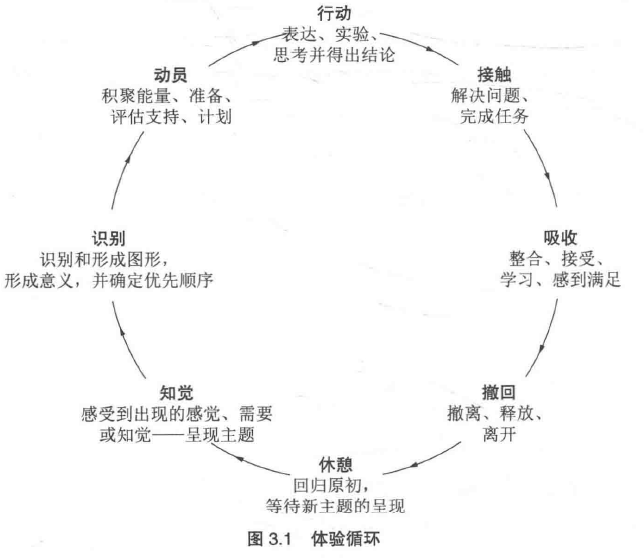
\includegraphics[width=\textwidth-11em]{aimg/2022-0406-1.jpg}
    \vspace{3pt}
\end{minipage}

\blockquote{
……一个居心叵测的女商人,刚刚完成一个收益颇丰的项目,立即就马不停蹄地寻找下一个项目或机会,无法享受闲暇,总担心如果顺其自然就会不进则退。(撤回与等待新图形出现之间的阻断)。

……一个循环完成之后到下一个主题呈现之前的阶段。这个阶段有时被称为“充实的休憩”( fertile void)。如此命名是为了强调纯粹的“存在于斯(being there)”,对自我保持充分而持续的觉察蓄势待发。……这是一种无欲、无知的状态,是主动放弃生物基本的控制欲望,也是完全放弃对未知的思维、情感、欲望、甚至信念的防御。

\citebook{格式塔咨询与治疗技术(第三版)}
}

沉默就像是休憩状态\pozhehao{}回归原初,等待新主题的呈现。在另一本书《弗里茨·皮尔斯:格式塔之父》里,fertile void被翻译为“盈空”\pozhehao{}“字面意思是‘丰富的空’,中译引用《道德经》中‘大盈若冲,其用不竭’的‘盈’字来表意‘fertile’。”

我会想起,在冥想的时候,自己也会经历一部分的体验循环,比如说知觉到一个想法或情感的出现,识别到那个想法或情感具体是什么,但没有动员、行动、接触和吸收,而是主动地撤回\pozhehao{}将自己的意识拉回到原来的锚点上(可以是自己的呼吸、周围的鸟鸣声等),然后进入盈空的状态:一片什么想法、什么情感都没有的虚无,甚至连自我意识的存在都消失了\pozhehao{}无我的状态。然后脑海里又会出现新的想法或情感,再继续这一体验循环。

但我想,冥想对于很多人而言并不是一种寻常的经历,沉默也是。

不过我也会想到,为什么是“盈空”,而不是“空”。

\blockquote{
尽管没有觉察到任何特别的东西,但这个人处于警觉状态,对所有的可能性开放。他的兴趣可能去向任何方向,此处亦或他方。他在平衡中,处于中间。他就任其自然。场还没有分化,图形和背景还是一体。

……在东方宗教中“无”(nothingness)意味着没有什么是实在的:只有过程、发生、纯粹的存在。现象学和存在主义哲学家也探索过“无”的概念,无来源于一种存在性恐惧,这种恐惧是因为意识到每个个体都是孤独的,终极意义并不存在而产生的。很多西方的普通人害怕并避免无的体验。存在主义思想认为,否认焦虑、死亡和无的现实的人,生活得不真实,皮尔斯受到这种思想的影响,提出面对存在性空可能是找到个人真实的手段。

皮尔斯不回避空,而是鼓励人们进入它并了解它。在他的第一本书中他用了一整章来教读者倾听其内在的寂静\pozhehao{}一种类似冥想的练习。他相信内在的寂静可以帮助一个人与其存在的更深的、直觉的层面接触。二十多年后,皮尔斯仍然用诗化的语言谈论空:“我们发现当我们接受、进人这种无、这个空的时候,沙漠开始开花。虚幻的空开始活跃,被充满。荒芜的空开始变成盈空。”

\citebook{格式塔咨询与治疗技术(第三版)}
}

“盈”可能更像是在指可能性的丰盈,虚无里蕴含着任何可能性的出现。只有经历了空,才会有新的体验循环,否则只是在循环着旧的体验,例如忙于开启看似新的话题、忙于和看似和新的恋人开始一段爱情,忙于追求一些看似不同却本质相同的体验。在同一个主题的体验循环里不断循环,体验变得僵硬,僵化为特定的、固定的模式。



% END LIST
% ======================================




\cleardoublepage
\pagestyle{empty}
\hspace{1pt}
\vfill
{
	\footnotesize
	\raggedright
	\sffamily
	\fontspec{Inter}


    \qrcode[link,height=30mm]{http://weixin.qq.com/r/sD8OChHEO9lHKVVpb2o0}
    \vspace{10mm}

    
    白色灯塔先生 \copyright{} 2022 版权所有

    \begin{description}[widest=,leftmargin=*,font=\mdseries\sffamily]%
        \item[构建日期] \today
        \item[装帧设计] Neruthes
    \end{description}
}
\end{document}
